
\documentclass[${FONT}pt $DRAFT]{$DOCUMENT} % ,draft

%%
%% Capture ENV vars from envsubst
%%

\def\AFIVE{$AFIVE}
\def\COMMITHASH{$COMMIT_HASH}
\def\COMMITTS{$COMMIT_TS}
\def\COVER{$COVER}
\def\DOMAIN{$DOMAIN}
\def\EBOOK{$EBOOK}
\def\EMAIL{$EMAIL}
\def\KINDLE{$KINDLE}
\def\LARGE{$LARGE}
\def\NARROW{$NARROW}
\def\PHONE{$PHONE}
\def\PRINT{$PRINT}
\def\QR{$QR}
\def\RIDERO{$RIDERO}
\def\DMK{$DMK}
\def\TABLET{$TABLET}

%%
%% Constants
%%

\def\NIL{}
\def\TRUE{true}

%%
%% if selectors
%%


%% http://handyfloss.net/2007.08/latex-programming-how-to-implement-conditionals/

%% QR

\newif\ifqr

\ifx\QR\TRUE
  \qrtrue
\else
  \qrfalse
\fi

%% NARROW

\newif\ifnarrow

\ifx\NARROW\TRUE
  \narrowtrue
\else
  \narrowfalse
\fi

%% KINDLE

\newif\ifkindle

\ifx\KINDLE\TRUE
  \kindletrue
\else
  \kindlefalse
\fi

%% TABLET

\newif\iftablet

\ifx\TABLET\TRUE
  \tablettrue
\else
  \tabletfalse
\fi


%% PHONE

\newif\ifphone

\ifx\PHONE\TRUE
  \phonetrue
\else
  \phonefalse
\fi

%% DMK

\newif\ifdmk

\ifx\DMK\TRUE
  \dmktrue
\else
  \dmkfalse
\fi

%% PRINT

\newif\ifprint

\ifx\PRINT\TRUE
  \printtrue
\else
  \printfalse
\fi

%% EBOOK

\newif\ifebook

\ifx\EBOOK\TRUE
  \ebooktrue
\else
  \ebookfalse
\fi

%% LARGE

\newif\iflarge

\ifx\LARGE\TRUE
  \largetrue
\else
  \largefalse
\fi

%% DMK

\newif\ifdmk

\ifx\DMK\TRUE
  \dmktrue
\else
  \dmkfalse
\fi

%% TITLE

\newif\iftitle

\ifx\TITLE\TRUE
  \titletrue
\else
  \titlefalse
\fi


% globals
\newlength{\marginparoffset}
\setlength{\marginparoffset}{0mm}


\usepackage[T2A]{fontenc}
\usepackage{tikz}
\usepackage{tocloft}
\usepackage{geometry}
\usepackage[utf8]{inputenc}
\usepackage[english,russian]{babel}


%% hyphenation in tt
\usepackage[shortcuts]{extdash}

% for proper ' and `
\usepackage{textcomp}
\usepackage{upquote}

% svg
\usepackage{svg}

% to replace strings
\usepackage{xstring}

% extra space at the end of macros
\usepackage{xspace}

% linebreaks in verbatim for mobile
\usepackage{spverbatim}

% http://www.khirevich.com/latex/microtype/
\usepackage[
  activate={true, nocompatibility},
  final,
  tracking=true,
  kerning=true,
  spacing=true,
  factor=1100,
  stretch=10,
  shrink=10
]{microtype}

% better captions
\usepackage[font=small]{caption}

\usepackage{float}

\captionsetup{labelsep=period}

\captionsetup[listing]{name=Листинг}
\captionsetup[figure]{name=Рис.}

% https://tex.stackexchange.com/a/417276
% ifthispageodd macro
\usepackage{scrextend}

% underline
\usepackage[normalem]{ulem}

% for QR codes in
\usepackage{qrcode}

% to have bold tt fonts in code listings
\usepackage{bold-extra}

% better macro args
\usepackage{xparse}

% file trees
\usepackage{dirtree}

%% defaults

%% offset = 0.2em
%% width = 1em
%% sep = 0.2em
%% rule-width = 0.4pt
%% dot-size = 1.6pt

% \setlength{\DTbaselineskip}{1.2em}

\DTsetlength{0.2em}{1em}{0.2em}{0.4pt}{0pt}


% code highlight
\usepackage[newfloat=true]{minted}
\usemintedstyle{print}
%% \setminted{fontsize=\small} %% reduce minted font
\SetupFloatingEnvironment{listing}{placement=H}

\ifnarrow
\setminted{breaklines=true}
\fi

% mobile headers
\ifnarrow
\usepackage{sectsty}
\sectionfont{\raggedright}
\subsectionfont{\raggedright}
\subsubsectionfont{\raggedright}
\fi

% index
\usepackage{index}
\newindex{default}{idx}{ind}{Предметный указатель}
\usepackage[
  unbalanced,
  itemlayout=abshang,
  indentunit=0.25em,
  totoc
]{idxlayout}
\ifnarrow
\idxlayout{columns=1}
\else
\idxlayout{columns=2}
\fi

\usepackage{setspace}


% href ursl for ebooks
\ifebook
\usepackage[hidelinks, hyperindex=false]{hyperref}
\fi


% no indent for items in lists (in mobile)
\ifnarrow
\usepackage{enumitem}
\setlist[itemize]{leftmargin=*}
\fi

%% geometry presets
\input{$GEOMETRY}

%% \geometry{showframe} %% debug frames

\setlength{\parskip}{0.32em}

\pagestyle{plain}
\pagenumbering{arabic}

\setcounter{tocdepth}{1}

\widowpenalty=10000
\clubpenalty=10000
\tolerance=500
\hyphenpenalty=500
\hfuzz=0.5pt
\emergencystretch=5pt


\usetikzlibrary{shapes.geometric, arrows, positioning, decorations.markings}

\ifnarrow
\tikzstyle{entity} = [rectangle, inner sep=3mm, minimum width=2.7cm, text centered, draw=black]
\else
\tikzstyle{entity} = [rectangle, inner sep=3mm, minimum width=3.0cm, text centered, draw=black]
\fi

\tikzstyle{arrow} = [thick,->,>=stealth,line width=0.4pt]

\tikzstyle{arrowHuge} = [thick, decoration={markings,mark=at position
   1 with {\arrow[semithick]{open triangle 60}}},
   double distance=1.4pt, shorten >= 5.5pt,
   preaction = {decorate},
   postaction = {draw,line width=1.4pt, white,shorten >= 4.5pt}]


\def\Plus{\texttt{+}}
\def\Minus{\texttt{-}}

\def\linegap{\vspace{1.25em}}

\def\arr{$\to$\xspace}

\def\enter{\textbf{Enter}}

\def\tilde{\raisebox{-1mm}{\textasciitilde{}}}

\newcommand{\slurp}{\vspace{-1em}}

\newcommand{\coderef}[1]{(строка~#1)\xspace}

\newcommand{\coderefs}[1]{(строки~#1)\xspace}

\newenvironment{teaser}{\vspace{-3em}\slshape}{\vspace{1em}}

\newcommand{\eng}[1]{(англ.~#1)}

\newcommand{\RNum}[1]{\uppercase\expandafter{\romannumeral #1\relax}}

% https://tex.stackexchange.com/questions/44361/
\DeclareTextFontCommand{\code}{\ttfamily\hyphenchar\font=45\relax}

\ifprint
\newcommand{\page}[1]{(с.~\pageref{#1})}
\newcommand{\fig}[1]{(рис.~\ref{#1})}
\newcommand{\lis}[1]{\xspace(листинг~\ref{#1})}
\fi

\ifebook
\newcommand{\page}[1]{\hyperref[#1]{\uline{(с.~\pageref{#1})}}}
\newcommand{\fig}[1]{\hyperref[#1]{\uline{(рис.~\ref{#1})}}}
\newcommand{\lis}[1]{\hyperref[#1]{\uline{(листинг~\ref{#1})}}}
\fi

\ifnarrow
\newcommand{\chart}[1]{\begin{center}\input{#1}\end{center}}
\else
\newcommand{\chart}[1]{\input{#1}}
\fi

\NewDocumentCommand{\pagebreaklarge}{O{4}}{\iflarge\pagebreak[#1]\fi}

\newcommand{\noindentnarrow}{\ifnarrow\noindent\fi}

\def\splitter{{\noindent\centering\rule{3cm}{.4pt}\par}}

\def\blank{\clearpage{\pagestyle{empty}\cleardoublepage}}

%% #1 text
%% #2 URL
%% #3 QR label
%% #4 offset
\ifprint
\NewDocumentCommand{\footurl}{ m m O{} o }{%
#1%
\footnote{\raggedright\StrSubstitute{#2}{https://}{}\ifdmk\hspace{0.1em}\tiny{.}\fi}%
\marginpar{%
\IfNoValueTF{#4}{}{\vspace{#4}}%
\vspace{-5.5mm}%
\ifthispageodd{\raggedright}{\raggedleft}%
\ifqr\qrcode[height=10mm]{#2}\else\begin{tikzpicture}
\draw (0,0) -- (1,0) -- (1,1) -- (0,1) -- (0,0);
\end{tikzpicture}
\fi%
\\\vspace{1mm}\tiny{#3}\vspace{12mm}}%
}%
\fi

\ifebook
\NewDocumentCommand{\footurl}{ m m O{} O{} }{\href{#2}{\uline{#1}}}
\fi

\newcommand{\smartlink}[2]{%
\ifprint
\texttt{#1}%
\fi
\ifebook
\href{#2}{\uline{#1}}%
\fi
}

\def\EMAILLINK{\smartlink{\EMAIL}{mailto:\EMAIL}}

\def\SITELINK{\smartlink{\DOMAIN}{https://\DOMAIN}}

%% small non-breaking space
%% https://tex.stackexchange.com/questions/76132/
\newcommand{\tuple}[1]{\textlangle\,#1\,\textrangle}

\newminted[clojure]{clojure}{}

\ifprint
\def\codeindent{0mm}
\fi

\ifebook
\def\codeindent{\parindent}
\fi

\newminted[clojure/lines]{clojure}{linenos, xleftmargin=\codeindent}

\newminted[xml/lines]{xml}{linenos, xleftmargin=\codeindent}

\newminted[text/lines]{text}{linenos, xleftmargin=\codeindent}

\newminted[python/lines]{python}{linenos, xleftmargin=\codeindent}

\newminted[json/lines]{json}{linenos, xleftmargin=\codeindent}

\newminted[sql/lines]{sql}{linenos, xleftmargin=\codeindent}

\newminted[yaml/lines]{yaml}{linenos, xleftmargin=\codeindent}

\newminted[json]{json}{}

\newminted[lisp]{lisp}{}

\newminted[yaml]{yaml}{}

\newminted[bash]{console}{}

\newminted[bash/lines]{bash}{linenos, xleftmargin=\codeindent}

\newminted[python]{python}{}

\newminted[htmldjango]{htmldjango}{}

\newminted[js]{js}{}

\newminted[java]{java}{}

\newminted[javascript]{javascript}{}

\newminted[php]{php}{}

\newminted[xml]{xml}{}

\newminted[diff]{diff}{}

\newminted[sql]{sql}{}

\newminted[http]{http}{}

\newminted[text]{text}{}

\newminted[ini]{ini}{}

\newenvironment{english}{\begin{otherlanguage}{english}}{\end{otherlanguage}}


\author{Иван Гришаев}
\title{Clojure на производстве. Том второй}
\date{}

\usepackage{pdfpages}

%%
%% Kindle or Phone
%%
\ifnarrow

%% Remove labels for subchapters
\usepackage{titlesec}
\titlelabel{}

%% Small page numbers
\usepackage{fancyhdr}
\fancypagestyle{plain}{
  \fancyhf{}
  \fancyfoot[C]{\tiny\thepage}}
\pagestyle{plain}

\fi

%% add space b/w number and footnote
\let\oldfootnote\footnote
\renewcommand\footnote[1]{\oldfootnote{\hspace{1mm}#1}}


%% for ebook, remove top margin for ToC
\ifebook
\setlength{\cftbeforetoctitleskip}{0pt}
\setlength{\cftaftertoctitleskip}{2em}
\fi

\begin{document}


\hyphenation{In-te-rac-ti-on}
\hyphenation{пред-шес-т-вен-ни-ка}
\hyphenation{пре-ды-ду-ще-го}
\hyphenation{Cre-a-te}
\hyphenation{Re-ad}
\hyphenation{Up-da-te}
\hyphenation{De-le-te}
\hyphenation{Java-Script}
\hyphenation{Chro-me}
\hyphenation{clo-ju-re}
\hyphenation{Clo-ju-re-Script}
\hyphenation{Cof-fee-Script}
\hyphenation{com-po-ju-re}
\hyphenation{com-po-nent}
\hyphenation{do-cu-men-ta-ti-on}
\hyphenation{au-to-comp-le-te}
\hyphenation{асинх-рон-ны-ми}
\hyphenation{брау-зер}
\hyphenation{вер-ну-ла}
\hyphenation{возвра-щает}
\hyphenation{возмож-нос-ти}
\hyphenation{дос-ту-па}
\hyphenation{дос-ту-пом}
\hyphenation{зави-си-мос-ти}
\hyphenation{зак-ры-ва-ет}
\hyphenation{зап-ро-са}
\hyphenation{зап-рос}
\hyphenation{ис-клю-че-ние}
\hyphenation{клиен-том}
\hyphenation{Фун-к-ц-ии}
\hyphenation{конф-ликт}
\hyphenation{крип-то-гра-фия}
\hyphenation{мно-жест-вен-ны-ми}
\hyphenation{наст-рой-ки}
\hyphenation{нейт-раль-ное}
\hyphenation{непус-тую}
\hyphenation{парал-лельно}
\hyphenation{пере-мен-ных}
\hyphenation{по-мес-тим}
\hyphenation{пов-тор}
\hyphenation{под-мно-жест-во}
\hyphenation{пос-ле}
\hyphenation{прик-лад-ных}
\hyphenation{проб-ле-му}
\hyphenation{проб-ле-мы}
\hyphenation{прог-рам-мис-тов}
\hyphenation{проек-та-ми}
\hyphenation{произ-водст-ва}
\hyphenation{проис-хо-дит}
\hyphenation{прост-ран-ство}
\hyphenation{разно-образ-ны}
\hyphenation{разоб-рать}
\hyphenation{реак-ци-ей}
\hyphenation{рес-то-ра-нов}
\hyphenation{свой-ства}
\hyphenation{сис-те-ма}
\hyphenation{сис-те-ме}
\hyphenation{систе-мах}
\hyphenation{систе-мы}
\hyphenation{следую-щий}
\hyphenation{соз-дай-те}
\hyphenation{соз-дать}
\hyphenation{сос-лать-ся}
\hyphenation{сос-то-ит}
\hyphenation{сос-тоя-ние}
\hyphenation{сох-ра-ни-ли}
\hyphenation{тес-тах}
\hyphenation{тес-тов}
\hyphenation{триг-рам-мный}
\hyphenation{удоб-ства}
\hyphenation{упрос-тит}
\hyphenation{фак-ти-чес-кое}
\hyphenation{цент-ра-ли-зо-ван}
\hyphenation{час-тя-ми}
\hyphenation{эко-сис-те-му}
\hyphenation{Throw-ab-le}
\hyphenation{middle-wa-re}
\hyphenation{ме-та-дан-ны-ми}
\hyphenation{con-text}
\hyphenation{проч-тут}
\hyphenation{Out-Of-Me-mo-ry-Er-ror}
\hyphenation{File-Not-Found-Excep-tion}
\hyphenation{Arithmetic-Exception}
\hyphenation{Null-Pointer-Exception}
\hyphenation{Il-legal-Argu-ment-Excep-tion}
\hyphenation{Byte-Array-Input-Stream}
\hyphenation{Excep-tion-Info}
\hyphenation{мес-тах}
\hyphenation{дейс-твие}
\hyphenation{замк-ну-та}
\hyphenation{vo-la-ti-le}
\hyphenation{пер-сис-тент-ны-ми}
\hyphenation{тес-ти-ро-ва-нии}
\hyphenation{наз-ва-ния}
\hyphenation{пос-то-ян-ных}
\hyphenation{до-пус-тить}
\hyphenation{не-до-пус-ти-мо}
\hyphenation{всег-да}
\hyphenation{тес-ты}
\hyphenation{прос-тей-ший}
\hyphenation{мес-та}
\hyphenation{интег-ра-ци-он-ное}
\hyphenation{Se-le-ni-um}
\hyphenation{File-Not-Found-Excep-tion}
\hyphenation{Сле-ду-ю-щий}
\hyphenation{не-сколь-ко}
\hyphenation{не-удач}
\hyphenation{не-ко-то-рые}
\hyphenation{прог-рам-ми-ро-ва-нии}
\hyphenation{раз-ны-ми}
\hyphenation{Ma-ni-fold}
\hyphenation{уст-рой-ст-вом}
\hyphenation{воз-вра-ща-ет}
\hyphenation{con-fig}
\hyphenation{PG-DA-TA-BA-SE}
\hyphenation{mo-unt}
\hyphenation{com-po-nent}
\hyphenation{Hi-ka-ri-CP}
\hyphenation{ме-то-дах}
\hyphenation{DE-LE-TE}
\hyphenation{chro-me-dri-ver}
\hyphenation{ge-cko-dri-ver}
\hyphenation{при-ло-же-ние}
\hyphenation{Unix-Port}
\hyphenation{Net-Port}
\hyphenation{trans-form}
\hyphenation{wat-cher}
\hyphenation{per-sis-tent}
\hyphenation{In-teg-rant}
\hyphenation{de-scrip-ti-on}
\hyphenation{name-spa-ces}
\hyphenation{get-ting}
\hyphenation{за-пус-ка-ет}
\hyphenation{Re-fe-ren-ce}
\hyphenation{Gui-des}
\hyphenation{Get-ting}
\hyphenation{Star-ted}
\hyphenation{лис-тин-ге}
\hyphenation{fix-tu-res}
\hyphenation{res-pon-se}
\hyphenation{Con-tent}
\hyphenation{Ty-pe}
\hyphenation{app-li-ca-ti-on}
\hyphenation{oc-tet}
\hyphenation{stre-am}
\hyphenation{pa-rams}
\hyphenation{me-ta-da-ta}
\hyphenation{da-ta-sour-ce}
\hyphenation{some-thing}
\hyphenation{re-defs}
\hyphenation{lo-ca-le}
\hyphenation{glo-bal}
\hyphenation{le-vel}
\hyphenation{Cont-rol-ler}
\hyphenation{init-db}
\hyphenation{mid-dle-wa-re}
\hyphenation{не-дос-тат-ки}
\hyphenation{ло-ка-ция}
\hyphenation{COM-MIT-TED}
\hyphenation{git-ig-no-re}
\hyphenation{если}
\hyphenation{свойстве}
\hyphenation{свойство}
\hyphenation{судя}
\hyphenation{англ}
\hyphenation{con-ti-nu-ous}
\hyphenation{in-teg-ra-ti-on}
\hyphenation{фун-к-ции}
\hyphenation{прог-рам-мис-тах}
\hyphenation{транз-ак-ци-я-ми}
\hyphenation{транз-ак-ции}


% add cover when set
\ifx\COVER\NIL
\else
\includepdf{\COVER}
\setcounter{page}{1}
\fi


% always add title page

\begin{titlepage}

\begin{center}

  {Иван Гришаев}

  \vspace*{5cm}

  {\Large\textbf{Clojure на производстве}}

  \vspace{1mm}

  {\Large\textbf{Зипперы, базы данных, REPL}}

  \vspace{7mm}

  {\Large Первое издание}

  {\small Редакция \COMMITHASH}

  \vspace*{\fill}

  \ifdmk
    
\includegraphics[width=20mm]{media/dmk_logo}%
    \linebreak{\small Москва, 2023}
  \else
    {2023}
  \fi

\end{center}

\end{titlepage}



% opening page (UDK & BBK) / annotation
\ifridero
  \iflarge
    \includepdf[pages={1}]{media/ridero_opening_large.pdf}
  \else
    \includepdf[pages={1}]{media/ridero_opening_normal.pdf}
  \fi
\else
 \thispagestyle{empty}

Продолжение книги <<Clojure на производстве>> об одноименном языке. В этот раз
мы рассмотрим обработку коллекций, работу с базой данных и обширное понятие
REPL. Материал нацелен на практику и отталкивается от реальных задач, которые
ждут в повседневной работе.

Как и первый том, книга не содержит азов изучения Clojure. Ожидается, что
читатель знаком с Clojure или другим промышленным языком. Для аудитории
продвинутого уровня.

\fi


% fix a widow line in TOC for A5
\ifafive
\setlength{\cftbeforetoctitleskip}{12mm}
\fi

% the same for large
\iflarge
\setlength{\cftbeforetoctitleskip}{25mm}
\fi

%%
%% ToC https://tex.stackexchange.com/questions/41555/
%%
\let\Contentsline\contentsline
\renewcommand\contentsline[3]{\thispagestyle{empty}\Contentsline{#1}{#2}{#3}}
\cleardoublepage
\tableofcontents


\newpage

\thispagestyle{empty}

\mbox{}


\clearpage

\section*{Об этой книге}

Перед вами второй том <<Clojure на производстве>>. Это продолжение первой книги,
которая вышла два года назад. Мы продолжим изучать Clojure~--- замечательный язык
с акцентом на неизменяемость и асинхронность. Clojure называют современным
Лиспом, потому что код на нем пишут S-выражениями — то есть со скобками.

По структуре и изложению книга не отличается от первой. Мы подробно рассмотрим
несколько тем, чередуя теорию с практикой. Каждая мысль в тексте подтверждается
кодом, и наоборот: сложный код разбит на части и подробно описан текстом.

Как и первый том, продолжение написано на русском языке. Автор много лет пишет
на Clojure и знаком с индустрией и~сообществом. Вас ждут привычные термины
вместо неуклюжих адаптаций. Все примеры и задачи автор взял из реальных
проектов; каждую строчку кода выполнил в REPL.

Коротко о том, что вас ждет. Первая глава расскажет о~зипперах в Clojure. Это
особый способ работы с коллекциями: непривычный, но крайне мощный. О зипперах
мало информации даже на английском языке, и книга закрывает этот недостаток.

Вторая глава посвящена реляционным базам данных, в основном PostgreSQL. Мы
рассмотрим основы SQL, подключение и работу с базой из Clojure. Автор учел все
наболевшие темы: построение сложных запросов, шаблонизацию SQL, работу с
выборкой и все то, о чем забывают другие руководства.

Третья глава охватывает сразу три смежные темы — REPL, Cider и Emacs. Читатель
узнает, что такое REPL и как подключиться к нему из редактора. Мы поговорим о
сетевом протоколе nREPL, о запуске проекта в Docker и на удаленной
машине. Рассмотрим REPL на платформе Javascript и проведем массу экспериментов.

В тексте мы не раз ссылаемся на первую книгу, особенно когда речь идет об
исключениях, системах или Clojure.spec. Это не помешает разобраться с темой,
даже если вы не читали первый том. Все же автор советует ознакомиться с ним для
лучшего понимания.

Книга рассчитана на продвинутую аудиторию. Желательно, чтобы у вас был опыт если
не с Clojure, то хотя бы с одним из промышленных языков. Пожелаем читателю
терпения, чтобы прочесть книгу до конца.

\section*{Код}

\def\urlcljbooksecond{https://github.com/igrishaev/clj-book2}

Исходный код книги в виде файлов \LaTeX{} находится в репозитории
\footurl{\code{igri\-sha\-ev/\-clj-book2}}{\urlcljbooksecond}[clj-book2][-1mm].
Если вы нашли опечатку, создайте pull request или issue с описанием проблемы.

\def\urlzipman{https://github.com/igrishaev/zipper-manual}

\def\urlbooksess{https://github.com/igrishaev/book-sessions}

Код первой главы о зипперах доступен в репозитории
\footurl{\code{igri\-sha\-ev/zip\-per-ma\-nu\-al}}{\urlzipman}[Zipper\\*manual]. Код
второй и третьей — в репозитории
\footurl{\code{igrishaev/book-sessions}}{\urlbooksess}[Book\\*sessions], пути
\code{src/book/db.clj} и \code{repl-chapter} соответственно.

Используйте код в любых целях, в том числе коммерческих.

\section*{Благодарности}

Автор благодарен стартапу \footurl{Clashapp}{https://huddlesapp.co}[Clashapp]
(ныне Huddles) и его коллективу за полученный опыт. Некоторые техники из этого
проекта нашли место в книге.

Спасибо читателям блога за присланные опечатки и уточнения. С ними текст удалось
улучшить до сдачи в печать.

Особая благодарность Андрею Листопадову за детальные отзывы к черновикам
глав. Посетите его сайт:
\footurl{andreyorst.gitlab.io}{https://andreyorst.gitlab.io}[Andrey\\*Orst].

\ifdmk
Благодарю коллектив издательства <<ДМК Пресс>> за то, что взяли рукопись в
работу. Их усилиями вы читаете эту книгу сейчас.
\fi

\ifridero
Благодарю коллектив издательства Rider\'{o} за то, что взяли рукопись в
работу. Их усилиями вы читаете эту книгу сейчас.
\fi

\section*{Обратная связь}

Присылайте ошибки и замечания на почту \EMAILLINK. Автор обновит
макет, и, возможно, следующий читатель получит исправленную версию книги.


%% \blank
\chapter{Зипперы}

\iflarge\vspace{3mm}\fi

\begin{teaser}
В этой главе мы рассмотрим зипперы в языке Clojure. Это необычный способ работы
с коллекциями. С помощью зиппера можно обойти произвольные данные, изменить их
или выполнить поиск. Зиппер~--- мощный инструмент, но вложения в него окупаются
со временем. Это сложная абстракция, которая требует подготовки.
\end{teaser}

\section{Азы навигации}

\index{зиппер}

Объясним зиппер простыми словами. Это обёртка над данными с набором
действий. Вот некоторые из них:

\begin{itemize}

\item
  перемещение по вертикали: вниз к потомкам или вверх к родителю;

\item
  перемещение по горизонтали: влево или вправо среди потомков;

\item
обход всех элементов;

\item
добавление, редактирование и удаление узлов.

\end{itemize}

Это неполный список того, что умеют зипперы. Другие их свойства мы
рассмотрим по ходу главы. Важно, что указанные действия относятся к любым
данным, будь то комбинация векторов и словарей, дерево узлов или XML. Из-за
этого зипперы становятся мощным инструментом. Разобраться с ними означает
повысить свои навыки и открыть новые двери.

\def\huet{https://en.wikipedia.org/wiki/Gerard\_Huet}
\def\huetzipper{https://www.st.cs.uni-saarland.de/edu/seminare/2005/advanced-fp/docs/huet-zipper.pdf}

Термин <<зиппер>> ввел ученый \footurl{Жерар Юэ}{\huet}[G\'{e}rard Huet][3mm]
(G\'{e}rard Huet) в 1996 году. Юэ занимался деревьями и искал универсальный
способ работы с ними. В знаменитой работе \footurl{<<Functional Pearl: The
  Zipper>>}{\huetzipper}[zipper.pdf] Юэ привел концепцию зиппера на языке
OCaml. Документ привлек внимание простотой и ясностью: описание зиппера, включая
код и комментарии, уместилось на четырёх страницах. Современные зипперы почти не
отличаются от того изложения 1996 года.

\index{Юэ, Жерар}

Хотя Юэ отмечает, что зиппер можно создать на любом языке, лучше всего они
прижились в функциональных: Haskell, OCaml, Clojure. Зипперы поощряют
неизменяемые данные и чистые преобразования. Для указанных языков написаны
библиотеки зипперов, в некоторых случаях больше одной. Наоборот, в императивной
среде зипперы почти неизвестны.

Зипперы доступны в Clojure с первой версии. Их легко добавить в проект, не
опасаясь проблем лицензии или новых зависимостей.

Зипперы в Clojure используют мощь неизменяемых коллекций. Технически зиппер~---
это коллекция, которая хранит данные и позицию в них. Всё вместе это называется
локацией (location). Шаг в любую сторону вернёт новую локацию подобно тому, как
функции \code{assoc} или \code{update} производят новые данные, оставляя прежние
нетронутыми.

\index{зиппер!локация}
\index{зиппер!узел}

Из текущей локации можно получить \emph{узел} (ноду)~--- данные, на которые ссылается
указатель. На этом месте путаются новички, поэтому уточним различие. Локация~---
это исходные данные и положение в них. Передвижение по локации порождает
локацию. Из локации можно извлечь узел~--- данные, которые встретились в локации.

\index{функции!zip/right}
\index{функции!zip/down}

Приведём пример с вектором \code{[1 2 3]}. Чтобы переместиться на
\textbf{двойку}, обернём данные в зиппер и выполним команды \code{zip/down} и
\code{zip/right}. С первым шагом мы провалимся в вектор и окажемся на
единице. Шаг вправо сдвинет нас на двойку.

Выразим это в коде: подключим модуль \code{clojure.zip} и переместимся по
вектору:

\begin{english}
  \begin{clojure}
(require '[clojure.zip :as zip])

(-> [1 2 3]
    zip/vector-zip
    zip/down
    zip/right
    zip/node)
;; 2
  \end{clojure}
\end{english}

Функция \code{zip/vector-zip} создаёт зиппер из вектора. Вызовы \code{zip/down} и
\code{zip/right} передвинут указатель на двойку, как и ожидалось. Последний шаг
\code{zip/node} вернёт значение (узел) текущей локации. Если убрать \code{zip/node},
получим локацию, которая соответствует двойке. Вот как она выглядит:

\begin{english}
  \begin{clojure}
(-> [1 2 3]
    zip/vector-zip
    zip/down
    zip/right)

[2 {:l [1]
    :pnodes [[1 2 3]]
    :ppath nil
    :r (3)}]
  \end{clojure}
\end{english}

Это пара, где первый элемент~--- значение, а второй~--- словарь направлений.

Наверняка у вас возникли вопросы: откуда мы знаем путь к двойке, ведь она могла
быть в другом месте вектора? Что произойдёт, если выйти за пределы коллекции?
Мы ответим на эти вопросы ниже. Пока что, если вам что-то не понятно, не
пугайтесь: мы не раз обсудим всё, что происходит.

Итак, зиппер предлагает перемещение по данным. Несмотря на всю мощь, он не
знает, как это делается для конкретной коллекции, и нуждается в вашей
помощи. Вот что нужно знать зипперу:

\begin{itemize}

\item
  является текущий элемент веткой или нет? Веткой называют элемент, из
  которого можно извлечь другие элементы;

\item
  если это ветка, как именно получить её элементы?

\end{itemize}

\pagebreaklarge

Как только мы знаем ответы на эти вопросы, зиппер готов. Заметим, что для
изменения зиппера нужен ответ на третий вопрос: как присоединить потомков к
ветке. Однако сейчас мы рассматриваем только навигацию, и третий вопрос
подождёт.

\index{функции!branch?}
\index{функции!children}

В техническом плане ответы на эти вопросы~--- функции. Первая принимает узел и
возвращает истину или ложь. Если получили истину, зиппер вызовет вторую функцию
с тем же узлом. От неё ожидают коллекцию дочерних узлов или \code{nil}, если их
нет. В терминах зиппера функции называют \code{branch?} и \code{children}
соответственно.

Чтобы получить зиппер, сообщите ему данные и эти две функции. Посколько мы
только читаем зиппер, третья функция будет \code{nil}.

\def\urlclojurezip{https://github.com/clojure/clojure/blob/master/src/clj/clojure/zip.clj}

Зипперы находятся в модуле \code{clojure.zip}; подключите его с псевдонимом
\code{zip}. В свободное время исследуйте код модуля: он занимает всего
\footurl{280 строк}{\urlclojurezip}[zip.clj]!

\begin{english}
  \begin{clojure}
(ns my.project
  (:require [clojure.zip :as zip]))
  \end{clojure}
\end{english}

Функция \code{zip/zipper} порождает зиппер из исходных данных и функций. Это
центральная точка модуля, его строительный материал. Для особых случаев модуль
содержит полуготовые зипперы, которые ожидают только данных. Примером служит
функция \code{vector-zip}. Она работает с вектором, элементы которого могут быть
другим вложенным вектором. Приведём её код в сокращении:

\index{функции!vector-zip}

\begin{english}
  \begin{clojure/lines}
(defn vector-zip
  [root]
  (zipper vector?
          seq
          ...
          root))
  \end{clojure/lines}
\end{english}

Третий параметр \coderef{5} мы заменили на многоточие. Это функция, которая присоединяет к
ветке дочерные узлы при изменении (пока что обходим вопрос стороной).

Если передать в \code{vector-zip} данные \code{[1 2 3]}, произойдёт
следующее. Зиппер обернёт вектор и выставит на него указатель. Из начального
положения можно следовать только вниз, потому что у вершины нет родителя (вверх)
и соседей (влево и вправо). При смещении \textbf{вниз} зиппер сначала проверит,
что текущий узел~--- ветка. Сработает выражение \code{(vector? [1 2 3])}, что
вернёт истину. В этом случае зиппер выполнит \code{(seq [1 2 3])}, чтобы
получить потомков. Ими станет последовательность \code{(1 2 3)}. Как только
потомки найдены, зиппер установит указатель на крайний левый потомок~---
единицу.

Покажем это на схеме. Начальная позиция, указатель на исходном векторе:

\begin{figure}[H]
  \centering
  \includesvg{charts/zip01.svg}
  \label{fig:chart-zip-01}
\end{figure}

Шаг вниз, указатель на единице:

\begin{figure}[H]
  \centering
  \includesvg{charts/zip02.svg}
  \label{fig:chart-zip-02}
\end{figure}

\pagebreaklarge

Шаг вправо, указатель на двойке:

\begin{figure}[H]
  \centering
  \includesvg{charts/zip03.svg}
  \label{fig:chart-zip-03}
\end{figure}

Итак, мы находимся в двойке и можем двигаться дальше по горизонтали. Шаг вправо
сдвинет нас на тройку, влево~--- на единицу. Вот как это выглядит в коде:

\begin{english}
  \begin{clojure}
(def loc2
  (-> [1 2 3]
      zip/vector-zip
      zip/down
      zip/right))

(-> loc2 zip/node)           ;; 2

(-> loc2 zip/right zip/node) ;; 3

(-> loc2 zip/left zip/node)  ;; 1
  \end{clojure}
\end{english}

При попытке сдвинуться вниз зиппер выполнит предикат \code{(vector? 2)}. Результат
будет ложью, что означает, что текущий элемент не ветка и движение вниз
запрещено.

Во время движения каждый шаг порождает новую локацию, не изменяя старую. Если вы
сохранили локацию в переменную, дальнейшие вызовы \code{zip/right} или
\code{zip/down} не изменят её. Выше мы объявили переменную \code{loc2}, которая
указывает на двойку. Проследуем от неё к исходному вектору:

\begin{english}
  \begin{clojure}
(-> loc2 zip/up zip/node)

;; [1 2 3]
  \end{clojure}
\end{english}

\pagebreaklarge

При ручном перемещении велики шансы выйти за пределы данных. Шаг в никуда вернёт
\code{nil} вместо локации:

\begin{english}
  \begin{clojure}
(-> [1 2 3]
    zip/vector-zip
    zip/down
    zip/left)
nil
  \end{clojure}
\end{english}

Это сигнал, что вы идёте по неверному пути. Из \code{nil} нельзя вернуться на
прежнее место, потому что у \code{nil} нет сведений о позиции. Для \code{nil}
функции \code{zip/up}, \code{zip/right} и другие тоже вернут \code{nil}. При
ручном перемещении проверяйте результат на \code{nil} или пользуйтесь оператором
\code{some->}:

\begin{english}
  \begin{clojure}
(some-> [1 2 3]
        zip/vector-zip
        zip/down
        zip/left
        zip/left
        ...)
;; nil
  \end{clojure}
\end{english}

К исключению относится функция \code{zip/down}: при попытке спуститься из \code{nil} вы
получите \code{NullPointerException}. Это недочёт, который, возможно, когда-нибудь
исправят.

\index{классы!NullPointerException}
\index{NullPointerException}

\begin{english}
  \begin{clojure}
(-> [1 2 3]
    zip/vector-zip
    zip/down
    zip/left
    zip/down)

;; Execution error (NullPointerException)...
  \end{clojure}
\end{english}

Как и в случае выше, от исключения вас убережёт макрос \code{some->}.

Рассмотрим случай, когда у вектора вложенные элементы: \code{[1 [2 3] 4]}. Чтобы
переместиться на \textbf{тройку}, выполним шаги <<вниз>>, <<вправо>>, <<вниз>>,
<<вправо>>. Сохраним локацию в переменную \code{loc3}:

\begin{english}
  \begin{clojure}
(def data
  [1 [2 3] 4])

(def loc3
  (-> data
      zip/vector-zip
      zip/down
      zip/right
      zip/down
      zip/right))

(zip/node loc3)

;; 3
  \end{clojure}
\end{english}

Рисунки ниже показывают, что происходит на каждом шаге. Исходная позиция:

\begin{figure}[H]
  \centering
  \includesvg{charts/zip04.svg}
  \label{fig:chart-zip-04}
\end{figure}

Шаг вниз:

\begin{figure}[H]
  \centering
  \includesvg{charts/zip05.svg}
  \label{fig:chart-zip-05}
\end{figure}

\pagebreaklarge

Вправо:

\begin{figure}[H]
  \centering
  \includesvg{charts/zip06.svg}
  \label{fig:chart-zip-06}
\end{figure}

Вниз:

\begin{figure}[H]
  \centering
  \includesvg{charts/zip07.svg}
  \label{fig:chart-zip-07}
\end{figure}

Вправо. Мы у цели:

\begin{figure}[H]
  \centering
  \includesvg{charts/zip08.svg}
  \label{fig:chart-zip-08}
\end{figure}

Чтобы перейти на \textbf{четвёрку} из текущей позиции, сначала поднимемся
вверх. Указатель сдвинется на вектор \code{[2 3]}. Мы находимся среди потомков
исходного вектора и можем перемещаться по горизонтали. Сделаем шаг вправо и
окажемся на цифре 4.

\pagebreaklarge

То же самое графически. Текущая локация (тройка):

\begin{figure}[H]
  \centering
  \includesvg{charts/zip09.svg}
  \label{fig:chart-zip-09}
\end{figure}

Шаг вверх:

\begin{figure}[H]
  \centering
  \includesvg{charts/zip10.svg}
  \label{fig:chart-zip-10}
\end{figure}

Шаг вправо:

\begin{figure}[H]
  \centering
  \includesvg{charts/zip11.svg}
  \label{fig:chart-zip-11}
\end{figure}

Исходный вектор может быть любой вложенности. Ради интереса замените данные на
\code{[5 [6 [7 [8] 9]]]} и проследуйте до девятки.

Что случится, если передать в \code{vector-zip} что-то отличное от вектора?
Предположим, \code{nil}, строку или число. Перед тем как двигаться, зиппер проверит,
подходит ли узел на роль ветки. Сработает функция \code{vector?}, которая вернёт
\code{nil} для всех отличных от вектора значений. В результате получим локацию, из
которой нельзя никуда шагнуть: ни вниз, ни в стороны. Это тупиковый случай, и
его нужно избегать.

\begin{english}
  \begin{clojure}
(-> "test"
    zip/vector-zip
    zip/down)
nil
  \end{clojure}
\end{english}

Модуль \code{clojure.zip} предлагает и другие встроенные зипперы. Особенно интересен
\code{xml-zip} для навигации по XML-дереву. Мы обсудим его отдельно, когда читатель
познакомится с другими свойствами зипперов.

\section{Автонавигация}

\index{навигация}

Мы разобрались с тем, как перемещаться по коллекции. Однако у читателя возникнет
вопрос: как мы узнаем заранее, куда двигаться? Откуда приходит путь?

Ответ покажется странным, но всё же: ручная навигация по данным лишена всякого
смысла. Если путь известен заранее, вам не нужен зиппер~--- это лишнее
усложнение.

Clojure предлагает более простую работу с данными, структура которых
известна. Например, если мы точно знаем, что на вход поступил вектор, второй
элемент которого~--- вектор, и нужно взять его второй элемент, то воспользуемся
\code{get-in}:

\begin{english}
  \begin{clojure}
(def data
  [1 [2 3] 4])

(get-in data [1 1])
;; 3
  \end{clojure}
\end{english}

То же самое касается других типов данных. Не важно, какую комбинацию образуют
списки и словари: если структура известна заранее, до элемента легко добраться с
помощью \code{get-in} или стрелочного оператора. В данном случае зипперы только
усложнят код.

\begin{english}
  \begin{clojure}
(def data
  {:users [{:name "Ivan"}]})

(-> data :users first :name)
;; "Ivan"
  \end{clojure}
\end{english}

В чем же тогда преимущество зипперов? Свои сильные стороны они проявляют там,
где \code{get-in} не работает. Речь о данных с \textbf{неизвестной}
структурой. Представьте, что на вход поступил произвольный вектор и нужно найти
в нём строку. Она может быть как на поверхности вектора, так и вложена на три
уровня. В~этом случае \code{get-in} не поможет, потому что мы не знаем путь.

Другой пример~--- XML-документ. Нужный тег может располагаться где угодно, и
нужно как-то его найти. Таким образом, идеальный случай для зиппера~--- нечёткая
структура данных, о которой у нас только предположения.

\index{функции!zip/up}
\index{функции!zip/down}
\index{функции!zip/next}

Функции \code{zip/up}, \code{zip/down} и другие образуют универсальную \code{zip/next}. Эта
функция передвигает указатель так, что рано или поздно мы обойдём всю
структуру. При обходе исключены повторы: мы побываем в каждом месте только
раз. Пример с вектором:

\begin{english}
  \begin{clojure}
(def vzip
  (zip/vector-zip [1 [2 3] 4]))

(-> vzip zip/node)
;; [1 [2 3] 4]

(-> vzip zip/next zip/node)
;; 1

(-> vzip zip/next zip/next zip/node)
;; [2 3]

(-> vzip zip/next zip/next zip/next zip/node)
;; 2
  \end{clojure}
\end{english}

Очевидно, мы не знаем, сколько раз вызывать \code{zip/next}, поэтому пойдём на
хитрость. Функция \code{iterate} принимает функцию \code{f} и значение \code{x}. Результатом
станет последовательность, где первый элемент \code{x}, а каждый следующий~--- \code{f(x)}
от предыдущего. Для зиппера мы получим исходную локацию, затем \code{zip/next} от
неё, потом \code{zip/next} от прошлого шага и так далее.

Переменная \code{loc-seq} ниже~--- это цепочка локаций исходного зиппера. Чтобы
получить узлы, мы берём шесть первых элементов (число взяли случайно) и вызываем
для каждого \code{zip/node}.

\begin{english}
  \begin{clojure}
(def loc-seq
  (iterate zip/next vzip))

(->> loc-seq
     (take 6)
     (map zip/node))

;; ([1 [2 3] 4], 1, [2 3], 2, 3, 4)
  \end{clojure}
\end{english}

\code{Iterate} порождает \textbf{ленивую} и \textbf{бесконечную}
последовательность. Обе характеристики важны. Ленивость означает, что очередной
сдвиг (вызов \code{zip/next}) не произойдёт до тех пор, пока вы не дойдёте до
элемента в цепочке. Бесконечность означает, что \code{zip/next} вызывается
неограниченное число раз. Понадобится признак, по которому мы остановим вызов
\code{zip/next}, иначе локации никогда не кончатся.

Если исследовать \code{loc-seq}, станет ясно, что в какой-то момент \code{zip/next} уже не
сдвигает указатель. Возьмём наугад сотый и тысячный элементы итерации. Их узел
будет исходным вектором:

\begin{english}
  \begin{clojure}
(-> loc-seq (nth 100) zip/node)

;; [1 [2 3] 4]

(-> loc-seq (nth 1000) zip/node)

;; [1 [2 3] 4]

  \end{clojure}
\end{english}

Причина кроется в устройстве зиппера. Функция \code{zip/next} работает по принципу
кольца. Когда она достигает исходной локации, цикл завершается. При этом локация
получит признак завершения, и дальнейший вызов \code{zip/next} вернёт её
же. Проверить признак можно функцией \code{zip/end?}:

\index{функции!zip/end?}

\begin{english}
  \begin{clojure}
(def loc-end
  (-> [1 2 3]
      zip/vector-zip
      zip/next
      zip/next
      zip/next))

loc-end
;; [[1 2 3] :end]

(zip/end? loc-end)
;; true

  \end{clojure}
\end{english}

Чтобы получить конечную цепь локаций, будем сдвигать указатель до тех пор, пока
локация не последняя. Всё вместе даёт функцию \code{iter-zip}:

\begin{english}
  \begin{clojure}
(defn iter-zip [zipper]
  (->> zipper
       (iterate zip/next)
       (take-while (complement zip/end?))))
  \end{clojure}
\end{english}

Функция вернёт все локации от начальной до конечной, не включая её. Напомним, что
локация хранит узел (элемент данных), который можно извлечь с помощью
\code{zip/node}. Код ниже показывает, как превратить локации в данные:

\begin{english}
  \begin{clojure}
(->> [1 [2 3] 4]
     zip/vector-zip
     iter-zip
     (map zip/node))

;; ([1 [2 3] 4], 1, [2 3], 2, 3, 4)
  \end{clojure}
\end{english}

Теперь, когда мы получили цепочку локаций, напишем поиск. Предположим, нужно
проверить, есть ли в векторе кейворд \code{:error}. Сначала напишем предикат для
локации~--- равен ли её узел этому значению:

\begin{english}
  \begin{clojure}
(defn loc-error? [loc]
  (-> loc zip/node (= :error)))
  \end{clojure}
\end{english}

Проверим, если ли среди локаций та, что подходит нашему предикату.  Для этого
вызовем \code{some}:

\begin{english}
  \begin{clojure}
(def data
  [1 [2 3 [:test [:foo :error]]] 4])

(some loc-error? (-> data
                     zip/vector-zip
                     iter-zip))
;; true
  \end{clojure}
\end{english}

Из-за ленивости мы не сканируем вектор целиком. Если нужный узел нашелся на
середине, \code{iter-zip} прекращает итерацию, и дальнейшие вызовы \code{zip/next} не
сработают.

Полезно знать, что \code{zip/next} обходит дерево в глубину. При движении он
стремится вниз и влево, а поднимается, лишь когда шаги в эти стороны
невозможны. Как мы увидим далее, в некоторых случаях порядок обхода
важен. Попадаются задачи, где мы должны двигаться вширь. По умолчанию в
\code{clojure.zip} нет других вариантов обхода, но мы напишем собственный. Также мы
рассмотрим задачу, где понадобится обход в ширину.

\index{функции!zip/vector-zip}

Встроенный зиппер \code{vector-zip} служит для вложенных векторов. Но гораздо
чаще встречаются вложенные словари. Напишем зиппер для обхода данных, как в
примере ниже:

\begin{english}
  \begin{clojure}
(def map-data
  {:foo 1
   :bar 2
   :baz {:test "hello"
         :word {:nested true}}})
  \end{clojure}
\end{english}

За основу возьмём знакомый нам \code{vector-zip}. Зипперы похожи, разница лишь в
типе коллекции. Подумаем, как задать функции \code{branch?} и
\code{children}. Сам по себе словарь~--- это ветка, чьи потомки~--- элементы
\code{MapEntry}. Тип \code{MapEntry} содержит ключ и значение. Если значение~---
словарь, получим из него цепочку вложенных \code{MapEntry} и так далее.

Для разминки напишем проверку на тип \code{MapEntry}:

\begin{english}
  \begin{clojure}
(def entry?
  (partial instance? clojure.lang.MapEntry))
  \end{clojure}
\end{english}

Зиппер \code{map-zip} выглядит так:

\begin{english}
  \begin{clojure/lines}
(defn map-zip [mapping]
  (zip/zipper
   (some-fn entry? map?)
   (fn [x]
     (cond
       (map? x)
       (seq x)
       (and (entry? x) (-> x val map?))
       (-> x val seq)))
   nil
   mapping))
  \end{clojure/lines}
\end{english}

Поясним основные моменты. Композиция \code{some-fn} \coderef{3} вернёт истину,
если хотя бы один из предикатов сработает положительно. Иными словами, на роль
ветки мы рассматриваем только словарь или его узел (пару ключ-значение).

Во второй функции, которая ищет потомков, приходится делать перебор. Для словаря
(проверка \code{map?}) получим потомков функцией \code{seq}~--- она вернёт цепочку
элементов \code{MapEntry}. Если текущий элемент~--- \code{MapEntry}, проверим, является ли
его значение вложенным словарём (функция \code{val} вернёт второй элемент
\code{MapEntry}). Если да, получим потомков той же функцией \code{seq}.

Обход зиппера вернёт все пары ключей и значений. Если значение~--- вложенный
словарь, мы провалимся в него при обходе. Пример:

\iflarge

\begin{english}
  \begin{clojure}
(->> {:foo 42
      :bar {:baz 11
            :user/name "Ivan"}}
     map-zip
     iter-zip
     rest
     (map zip/node))
  \end{clojure}
\end{english}

\begin{english}
  \begin{clojure}
([:foo 42]
 [:bar {:baz 11, :user/name "Ivan"}]
 [:baz 11]
 [:user/name "Ivan"])
  \end{clojure}
\end{english}

\else

\begin{english}
  \begin{clojure}
(->> {:foo 42
      :bar {:baz 11
            :user/name "Ivan"}}
     map-zip
     iter-zip
     rest
     (map zip/node))

;; ([:foo 42]
;;  [:bar {:baz 11, :user/name "Ivan"}]
;;  [:baz 11]
;;  [:user/name "Ivan"])
  \end{clojure}
\end{english}

\fi

Обратите внимание на функцию \code{rest} после \code{iter-zip} \coderef{6}. Мы
отбросили первую локацию, в которой находятся исходные данные. Они известны,
поэтому нет смысла печатать их.

С помощью нашего \code{map-zip} легко проверить, есть ли в словаре ключ
\code{:error} со значением \code{:auth}. По отдельности эти кейворды могут быть
где угодно~--- в ключах или значениях на любом уровне. Однако нас интересует их
комбинация. Для этого напишем предикат:

\begin{english}
  \begin{clojure}
(defn loc-err-auth? [loc]
  (-> loc zip/node (= [:error :auth])))
  \end{clojure}
\end{english}

Убедимся, что в первом словаре нет пары, даже несмотря на то, что значения
встречаются по отдельности:

\begin{english}
  \begin{clojure}
(->> {:response {:error :expired
                 :auth :failed}}
     map-zip
     iter-zip
     (some loc-err-auth?))

;; nil
  \end{clojure}
\end{english}

Но даже если пара вложена глубоко, мы найдём её:

\begin{english}
  \begin{clojure}
(def data
  {:response {:info {:message "Auth error"
                     :error :auth
                     :code 1005}}})

(->> data
     map-zip
     iter-zip
     (some loc-err-auth?))

;; true
  \end{clojure}
\end{english}

Предлагаем читателю несколько заданий для самостоятельной работы.

\begin{enumerate}

\item
  Зиппер \code{map-zip} не учитывает случай, когда ключ словаря~--- другой словарь,
  например:

\begin{english}
  \begin{clojure}
{{:alg "MD5" :salt "..."} "deprecated"
 {:alg "SHA2" :salt "..."} "deprecated"
 {:alg "HMAC-SHA256" :key "..."} "ok"}
  \end{clojure}
\end{english}

Такие коллекции хоть и редко, но встречаются в практике. Доработайте \code{map-zip},
чтобы он проверял не только значение \code{MapEntry}, но и ключ (вместо \code{val}
используйте \code{key}).

\item
  Мы рассмотрели зипперы для векторов и словарей по отдельности. На практике
  работают со смешанными данными, когда словари и векторы вложены друг в
  друга. Напишите универсальный зиппер, который учитывает обе коллекции при
  обходе.

\end{enumerate}

\section{XML-зипперы}

\index{XML}

Мощь зипперов раскрывается в полной мере при работе с XML. От других форматов он
отличается тем, что задан рекурсивно. Например, в JSON объект и массив выглядят
по-разному. То же самое относится с YAML, где у каждого типа свои синтаксис и
структура. В XML, где бы мы ни находились, текущий узел состоит из трёх
элементов: тега, атрибутов и содержимого.

Тег~--- это короткое имя узла, например \code{name} или \code{description}. Атрибуты~---
словарь свойств и значений. Наиболее интересно содержимое: это набор строк
или других узлов. Вот как выглядит XML на псевдокоде:

\begin{english}
  \begin{text}
XML = [Tag, Attrs, [String|XML]]
  \end{text}
\end{english}

Чтобы убедиться в однородности XML, рассмотрим файл с товарами поставщиков. На
вершине XML находится узел \code{catalog}. Это группировочный тег: он необходим,
потому что на вершине не может быть несколько тегов. Потомки каталога~---
организации. В атрибуте \code{name} организации указано её имя. Под организацией
идут товары~--- узлы с тегом \code{product} и атрибутом \code{type}. Вместо
потомков товар содержит текст~--- его наименование. Ниже товара спуститься уже
нельзя.

\begin{english}
  \begin{xml}
<?xml version="1.0" encoding="UTF-8"?>
<catalog>
  <organization name="re-Store">
    <product type="iphone">iPhone 11 Pro</product>
    <product type="iphone">iPhone SE</product>
  </organization>
  <organization name="DNS">
    <product type="tablet">iPad 3</product>
    <product type="notebook">Macbook Pro</product>
  </organization>
</catalog>
  \end{xml}
\end{english}

Clojure предлагает XML-парсер, который вернёт структуру, похожую на схему
\code{[Tag, Attrs, Content]} выше. Каждый узел станет словарём с ключами
\code{:tag}, \code{:attrs} и \code{:content}. Последний хранит вектор, где
элемент~--- либо строка, либо вложенный словарь.

Поместим XML с товарами в файл \code{resources/products.xml}. Напишем функцию
\code{->xml-zipper}, чтобы считать файл в зиппер. Добавьте модули \code{xml} и
\code{io}:

\begin{english}
  \begin{clojure}
(:require
 [clojure.java.io :as io]
 [clojure.xml :as xml])
  \end{clojure}
\end{english}

Оба входят в поставку Clojure и не требуют зависимостей. Чтобы получить зиппер,
пропустим параметр \code{path} через серию функций:

\index{функции!xml/parse}
\index{функции!zip/xml-zip}

\begin{english}
  \begin{clojure}
(defn ->xml-zipper [path]
  (-> path
      io/resource
      io/file
      xml/parse
      zip/xml-zip))
  \end{clojure}
\end{english}

Функция \code{xml/parse} вернёт структуру словарей с ключами \code{:tag},
\code{:attrs} и \code{:content}. Обратите внимание, что текстовое содержимое
(например, название товара)~--- это тоже вектор с одной строкой. Тем самым
достигается однородность узлов на всех уровнях.

Вот что получим после вызова \code{xml/parse}:

\begin{english}
  \begin{clojure}
{:tag :catalog
 :attrs nil
 :content
 [{:tag :organization
   :attrs {:name "re-Store"}
   :content
   [{:tag :product
     :attrs {:type "iphone"}
     :content ["iPhone 11 Pro"]}
    {:tag :product
     :attrs {:type "iphone"}
     :content ["iPhone SE"]}]}
  {:tag :organization
   :attrs {:name "DNS"}
   :content
   [{:tag :product
     :attrs {:type "tablet"}
     :content ["iPad 3"]}
    {:tag :product
     :attrs {:type "notebook"}
     :content ["Macbook Pro"]}]}]}
  \end{clojure}
\end{english}

Вызов \code{(->xml-zipper "products.xml")} вернёт первую локацию зиппера
XML. Прежде чем работать с ним, заглянем в определение \code{zip/xml-zip}, чтобы
понять, что происходит. Приведём его код в сокращении:

\begin{english}
  \begin{clojure}
(defn xml-zip [root]
  (zipper (complement string?)
          (comp seq :content)
          ...
          root))
  \end{clojure}
\end{english}

Очевидно, потомки узла~--- это его содержимое \code{:content}, дополнительно обёрнутое
в \code{seq}. У строки не может быть потомков, поэтому \code{(complement string?)}
означает: искать потомков в узлах, отличных от строки.

Рассмотрим, как бы мы нашли все товары из заданного XML. Для начала получим
ленивую итерацию по зипперу. Напомним, что на каждом шаге мы получим не словарь
с полями \code{:tag} и другими, а локацию с указателем на него. Останется
выбрать локации, чьи узлы содержат тег \code{product}. Для этого напишем
предикат:

\begin{english}
  \begin{clojure}
(defn loc-product?
  [loc]
  (-> loc zip/node :tag (= :product)))
  \end{clojure}
\end{english}

Выборка с преобразованием:

\begin{english}
  \begin{clojure}
(->> "products.xml"
     ->xml-zipper
     iter-zip
     (filter loc-product?)
     (map loc->product))

;; ("iPhone 11 Pro"
;;  "iPhone SE"
;;  "iPad 3"
;;  "Macbook Pro")
  \end{clojure}
\end{english}

На первый взгляд здесь ничего особенного. Структура XML известна заранее,
поэтому можно обойтись без зиппера. Для этого выберем потомков каталога и
получим организации; из потомков организаций получим товары. Вместе получится
простой код:

\index{функции!mapcat}

\begin{english}
  \begin{clojure}
(def xml-data
  (-> "products.xml"
      io/resource
      io/file
      xml/parse))

(def orgs
  (:content xml-data))

(def products
  (mapcat :content orgs))

(def product-names
  (mapcat :content products))
  \end{clojure}
\end{english}

\pagebreaklarge

Для краткости уберём переменные и сведём код к одной форме:

\begin{english}
  \begin{clojure}
(->> "products.xml"
     io/resource
     io/file
     xml/parse
     :content
     (mapcat :content)
     (mapcat :content))

;; ("iPhone 11 Pro"
;;  "iPhone SE"
;;  "iPad 3"
;;  "Macbook Pro")
  \end{clojure}
\end{english}

На практике структура XML неоднородна. Предположим, крупный поставщик разбивает
товары по филиалам. В его случае XML выглядит так (фрагмент):

\begin{english}
  \begin{xml}
<organization name="DNS">
  <branch name="Office 1">
    <product type="tablet">iPad 3</product>
    <product type="notebook">Macbook Pro</product>
  </branch>
</organization>
  \end{xml}
\end{english}

Код выше, где мы слепо выбираем данные по уровню, сработает неверно. В списке
товаров окажется узел:

\begin{english}
  \begin{clojure}
("iPhone 11 Pro"

 "iPhone SE"

 {:tag :product
  :attrs {:type "tablet"}
  :content ...})
  \end{clojure}
\end{english}

В то время как зиппер вернёт \textbf{только} товары, в том числе из филиала:

\pagebreaklarge

\begin{english}
  \begin{clojure}
(->> "products-branch.xml"
     ->xml-zipper
     iter-zip
     (filter loc-product?)
     (map loc->product))

;; ("iPhone 11 Pro"
;;  "iPhone SE"
;;  "iPad 3"
;;  "Macbook Pro")
  \end{clojure}
\end{english}

Очевидно, выгодно пользоваться кодом, который работает с обоими XML, а не
поддерживать отдельную версию для крупного поставщика. В противном случае нужно
где-то хранить признак и делать по нему \code{if/else}, что усложнит проект.

\index{функции!xml-seq}

Однако этот пример не раскрывает всю мощь зипперов. Для обхода XML уже есть
готовое средство~--- функция \code{xml-seq} из главного модуля Clojure. Она
возвращает ленивую цепочку XML-узлов в том же виде (словари с ключами
\code{:tag}, \code{:attr} и \code{:content}). \code{Xml-seq}~--- это частный
случай более абстрактной функции \code{tree-seq}. Последняя похожа на зиппер
тем, что принимает функции \code{branch?} и \code{children}, чтобы определить,
подходит ли узел на роль ветки и как извлечь потомков. Определение
\code{xml-seq} напоминает \code{xml-zip}:

\begin{english}
  \begin{clojure}
(defn xml-seq
  "A tree seq on the xml elements as per xml/parse"
  {:added "1.0"
   :static true}
  [root]
  (tree-seq (complement string?)
            (comp seq :content)
            root))
  \end{clojure}
\end{english}

Разница между зиппером и \code{tree-seq} в том, что при обходе зиппер возвращает
локацию~--- элемент, в котором больше сведений. Кроме данных, он содержит ссылки
на элементы по всем четырём направлениям. Наоборот, \code{tree-seq} итерирует
данные без обёрток. Для обычного поиска \code{tree-seq} даже предпочтительней,
поскольку не порождает лишних абстракций. Вот как выглядит сбор товаров с учётом
филиалов:

\pagebreaklarge

\begin{english}
  \begin{clojure}
(defn node-product? [node]
  (some-> node :tag (= :product)))

(->> "products-branch.xml"
     io/resource
     io/file
     xml/parse
     xml-seq
     (filter node-product?)
     (mapcat :content))

("iPhone 11 Pro" "iPhone SE" "iPad 3" "Macbook Pro")
  \end{clojure}
\end{english}

Чтобы показать мощь зипперов, подберём такую задачу, где возможностей \code{tree-seq}
не хватает. На эту роль подойдёт поиск с переходом между локациями.

\section{Поиск в XML}

\index{XML!поиск}

Предположим, нам поставили задачу: выбрать из XML магазины, где продаются
айфоны. Обратите внимание: мы впервые коснулись связи между узлами, и это
важно. По отдельности выбрать данные легко. Магазины~--- это локации, у которых
тег \code{organization}. Айфоны~--- локации, в которых узел с тегом \code{product} и
атрибутом \code{type="iphone"}. Но как найти связь между ними?

В прошлый раз мы разложили XML в последовательность с помощью
\code{xml-seq}. Проблема в том, что функция порождает коллекцию узлов без какой-либо
связи, что не даёт нам решить задачу. Покажем это на примере. Для начала получим
цепочку узлов:

\begin{english}
  \begin{clojure}
(def xml-nodes
  (->> "products-branch.xml"
       io/resource
       io/file
       xml/parse
       xml-seq))
  \end{clojure}
\end{english}

Вообразим, что в одном из элементов находится нужный товар. Например, мы
встретили айфон в третьем (втором от нуля) узле:

\begin{english}
  \begin{clojure}
(-> xml-nodes (nth 2))
;; {:tag :product
;;  :attrs {:type "iphone"}
;;  :content ["iPhone 11 Pro"]}
  \end{clojure}
\end{english}

Однако не ясно, как найти магазин, которому он принадлежит. Можно предположить,
что магазин находится слева от товара, потому что предшествует ему при
обходе. Это станет ясно, если напечатать теги узлов:

\begin{english}
  \begin{clojure}
(->> xml-nodes
     (mapv :tag)
     (remove nil?)
     (run! print))

;; :catalog :organization :product :product ...
  \end{clojure}
\end{english}

Идея верная, но в целом слабая, потому что зависит от порядка обхода. Кроме
того, задача усложняется: при обходе нужно не просто выбрать нужные товары, но и
переместиться назад в поисках магазина. Затем продолжить вперед и при этом
пропустить найденный товар, чтобы не попасть в вечный цикл.

Здесь и приходит на помощь зиппер. Локация, которую он возвращает на каждом
шаге, помнит положение в структуре. От локации можно пройти в нужное место с
помощью функций \code{zip/up}, \code{zip/right} и других, что мы рассмотрели в
начале главы. Это тот случай, когда ручная навигация оправдана.

\index{функции!zip/right}

Вернёмся к XML со структурой <<каталог~--- организация~--- товары>>. Освежим его в
памяти:

\begin{english}
  \begin{xml}
<?xml version="1.0" encoding="UTF-8"?>
<catalog>
  <organization name="re-Store">
    <product type="iphone">iPhone 11 Pro</product>
    <product type="iphone">iPhone SE</product>
  </organization>
  <organization name="DNS">
    <product type="tablet">iPad 3</product>
    <product type="notebook">Macbook Pro</product>
  </organization>
</catalog>
  \end{xml}
\end{english}

Прежде всего найдём локации-айфоны. Напишем предикат на айфон:

\begin{english}
  \begin{clojure}
(defn loc-iphone? [loc]
  (let [node (zip/node loc)]
    (and (-> node :tag (= :product))
         (-> node :attrs :type (= "iphone")))))
  \end{clojure}
\end{english}

Получим локации с айфонами:

\begin{english}
  \begin{clojure}
(def loc-iphones
  (->> "products.xml"
       ->xml-zipper
       iter-zip
       (filter loc-iphone?)))

(count loc-iphones)
2
  \end{clojure}
\end{english}

Теперь, чтобы найти организацию по товару, поднимемся на уровень выше с помощью
\code{zip/up}. Это верно, потому что организация~--- родитель товара:

\begin{english}
  \begin{clojure}
(def loc-orgs
  (->> loc-iphones
       (map zip/up)
       (map (comp :attrs zip/node))))

({:name "re-Store"}
 {:name "re-Store"})
  \end{clojure}
\end{english}

Для каждого айфона мы нашли организацию, где его продают. Получились дубли,
потому что оба айфона продаются в re-Store. Чтобы избавиться от повторов,
оберните результат в \code{set}.

\begin{english}
  \begin{clojure}
(set loc-orgs)

#{{:name "re-Store"}}
  \end{clojure}
\end{english}

Это и есть ответ на вопрос: айфоны можно купить в магазине re-Store. Если
добавить айфон в организацию DNS, она тоже появится в \code{loc-orgs}.

Решим ту же задачу для XML с филиалами. Теперь мы не можем вызвать \code{zip/up}
для товара, чтобы получить организацию, потому что в некоторых случаях получим
филиал, и понадобится ещё один шаг вверх. Чтобы не гадать, сколько раз
подниматься, напишем функцию \code{loc->org}. Она вызывает \code{zip/up} до тех
пор, пока не выйдет на нужный тег:

\begin{english}
  \begin{clojure}
(defn loc-org? [loc]
  (-> loc zip/node :tag (= :organization)))

(defn loc->org [loc]
  (->> loc
       (iterate zip/up)
       (find-first loc-org?)))
  \end{clojure}
\end{english}

Функция \code{find-first} находит первый элемент коллекции, который подошёл
предикату. Она ещё не раз пригодится нам.

\begin{english}
  \begin{clojure}
(defn find-first [pred coll]
  (some (fn [x]
          (when (pred x)
            x))
        coll))
  \end{clojure}
\end{english}

Чтобы сократить код, не будем объявлять переменные \code{loc-iphones} и
другие. Выразим поиск одной формой:

\begin{english}
  \begin{clojure/lines}
(->> "products-branch.xml"
     ->xml-zipper
     iter-zip
     (filter loc-iphone?)
     (map loc->org)
     (map (comp :attrs zip/node))
     (set))

;; #{{:name "re-Store"}}
  \end{clojure/lines}
\end{english}

Новое решение отличается лишь тем, что мы заменили \code{zip/up} на функцию с более
сложным восхождением \coderef{5}. В остальном ничего не изменилось.

\index{JSON}

Обратите внимание, насколько удобен XML в плане поиска и навигации. Если хранить
данные в JSON, их структура и обход отличаются кардинально. Это будут различные
комбинации векторов и объектов, которые трудно подчинить единым правилам. Для
работы с ними нужен разный код. В случае с XML его структура однородна:
добавление филиала меняет лишь глубину товаров, но не правила обхода.

Усложним задачу: среди обычных товаров встречаются наборы (bundle). Товар из
набора нельзя купить отдельно. Например, тряпочка для экрана продаётся чаще
всего с устройством \coderef{10}. Нас просят найти магазин, где тряпочку можно
купить отдельно \coderef{4}. Пример XML, в котором мы будем искать:

\begin{english}
  \begin{xml/lines}
<?xml version="1.0" encoding="UTF-8"?>
<catalog>
  <organization name="re-Store">
    <product type="fiber">VIP Fiber Plus</product>
    <product type="iphone">iPhone 11 Pro</product>
  </organization>
  <organization name="DNS">
    <branch name="Office 2">
      <bundle>
        <product type="fiber">Premium iFiber</product>
        <product type="iphone">iPhone 11 Pro</product>
      </bundle>
    </branch>
  </organization>
</catalog>
  \end{xml/lines}
\end{english}

Сначала найдём все тряпочки. В них окажутся как отдельные товары, так и из
набора:

\begin{english}
  \begin{clojure}
(defn loc-fiber? [loc]
  (some-> loc
          zip/node
          (get-in [:attrs :type])
          (= "fiber")))

(->> "products-bundle.xml"
     ->xml-zipper
     iter-zip
     (filter loc-fiber?)
     (map (comp first :content zip/node)))

;; ("VIP Fiber Plus" "Premium iFiber")
  \end{clojure}
\end{english}

Теперь решим задачу. Из найденных тряпочек отсекаем те, что входят в набор. С
точки зрения зиппера это значит, что у родителя этой локации тег \emph{не равен}
\code{:bundle}. От оставшихся тряпочек переходим к магазинам.

Введём предикат \code{loc-in-bundle?}~--- входит локация в набор или нет:

\begin{english}
  \begin{clojure}
(defn loc-in-bundle?
  [loc]
  (some-> loc
          zip/up
          zip/node
          :tag
          (= :bundle)))
  \end{clojure}
\end{english}

Решение:

\begin{english}
  \begin{clojure}
(->> "products-bundle.xml"
     ->xml-zipper
     iter-zip
     (filter loc-fiber?)
     (remove loc-in-bundle?)
     (map loc->org)
     (map (comp :attrs zip/node))
     (set))

#{{:name "re-Store"}}
  \end{clojure}
\end{english}

Магазин DNS не попал в результат, потому что в нём тряпочка продаётся в наборе.

Новое усложнение: мы хотим купить айфон, \emph{но только в наборе} с тряпочкой. В
какой магазин направить покупателя?

Решение: сначала ищем все айфоны. Оставляем те, что входят в набор. Среди
соседей айфона ищем тряпочку. Если нашли, переходим от айфона или тряпочки к
магазину. Основные функции уже готовы: это предикаты на проверку набора, тип
товара и другие мелочи. Но мы не рассмотрели, как получить соседей локации.

Функции \code{zip/lefts} и \code{zip/rights} вернут элементы по левую и правую
стороны от текущей локации. Совместим их через \code{concat}, чтобы получить
всех соседей:

\begin{english}
  \begin{clojure}
(defn node-neighbors [loc]
  (concat (zip/lefts loc)
          (zip/rights loc)))
  \end{clojure}
\end{english}

Уточним, что это будут именно элементы, а не локации. Покажем это на примере
вектора и локации с числом 2. Её соседями будут числа 1 и 3:

\begin{english}
  \begin{clojure}
(-> [1 2 3]
    zip/vector-zip
    zip/down
    zip/right
    node-neighbors)

;; (1 3)
  \end{clojure}
\end{english}

Зиппер устроен так, что получить правые и левые элементы проще, чем передвигать
локацию влево или вправо. Поэтому при поиске среди соседей выгодно работать с
элементами, а не локациями.

Добавим функции, чтобы проверить, есть ли в соседях локации тряпочка:

\begin{english}
  \begin{clojure}
(defn node-fiber?
  [node]
  (some-> node :attrs :type (= "fiber")))

(defn with-fiber?
  [loc]
  (let [nodes (node-neighbors loc)]
    (find-first node-fiber? nodes)))
  \end{clojure}
\end{english}

Готовая функция:

\begin{english}
  \begin{clojure}
(defn shops-by-iphone-with-fiber [filepath]
  (->> filepath
       ->xml-zipper
       iter-zip
       (filter loc-iphone?)
       (filter loc-in-bundle?)
       (filter with-fiber?)
       (map loc->org)
       (map (comp :name :attrs zip/node))
       (set)))

(shops-by-iphone-with-fiber "products-bundle.xml")

;; #{"DNS"}
  \end{clojure}
\end{english}

В результате получим магазин DNS, потому что именно в нём айфон продается в
комплекте с тряпочкой. Оба товара продаются в re-Store по отдельности, что не
подходит условию задачи.

Можно добавить больше ограничений. Например, из найденных магазинов выбрать те,
что расположены в радиусе 300 метров от покупателя. Для этого понадобятся
расположение магазинов на карте и функция попадания точки в окружность. Можно
выбрать только открытые магазины или те, что предлагают доставку. Запишем эти
признаки в атрибуты организаций и добавим функции отбора.

Легко увидеть, что XML-зиппер стал настоящей базой данных. Он даёт ответы на
сложные запросы, при этом код растёт медленнее, чем их смысловая нагрузка. Из-за
рекурсивной структуры XML хорошо поддается обходу, и зипперы усиливают это
преимущество. Обратите внимание, как удобно работают переходы и связи между
узлами. Представьте, каких усилий стоило бы разбить данные на таблицы и писать
SQL с оператором JOIN.

Конечно, по сравнению с настоящей базой данных у XML недостаток~--- в нём нет
индексов, и поиск работает линейным перебором, а не как в бинарных
деревьях. Кроме того, наш подход требует, чтобы данные находились в памяти
целиком. Он не сработает для очень больших документов с миллионами записей, но
пока что не будем волноваться об этом.

\section{Редактирование}

До сих пор мы игнорировали другую возможность зипперов. Во~время обхода можно не
только читать, но и менять локации. В~широком плане нам доступны все операции
CRUD (Create, Read, Update, Delete), знакомые из веб-разработки. Ниже мы
разберём, как они работают в зипперах.

\index{зиппер!редактирование}

Напомним, зиппер принимает третью функцию \code{make-node}, в которую до сих пор мы
передавали \code{nil}. В ней не было нужды, потому что мы только читали
данные. Зиппер вызовет функцию в момент, когда мы просим вернуть данные с учётом
изменений, которые внесли в локации. Функция принимает два параметра: ветку и
потомков. Её задача~--- соединить их должным образом.

Для простых коллекций вроде вектора функция проста~--- нужно только обернуть
потомков в \code{vec}, чтобы получить из последовательности вектор. В \code{vector-zip}
функция чуть сложнее, потому что учитывает метаданные. Приведём код этого
зиппера без сокращений:

\index{метаданные}

\begin{english}
  \begin{clojure/lines}
(defn vector-zip
  [root]
  (zipper vector?
          seq
          (fn [node children]
            (with-meta (vec children) (meta node)))
          root))
  \end{clojure/lines}
\end{english}

Видим, что новый вектор \coderef{6} копирует метаданные прежнего вектора
(переменная \code{node}). Если дополнить оригинал через \code{assoc} или
\code{conj}, метаданные сохраняются. В случае с \code{vector-zip} мы строим
новый вектор, поэтому оборачиваем его в \code{with-meta}. Если убрать
\code{with-meta}, на выходе получим вектор без метаданных, что может повлиять на
логику программы.

У XML-зиппера сборка иная: потомков помещают в поле \code{:content}.

\begin{english}
  \begin{clojure}
(fn [node children]
  (assoc node :content
              (and children (apply vector children))))
  \end{clojure}
\end{english}

Для нашего \code{map-zip}, который работает со словарями, функция сборки выглядела бы
как \code{assoc} или \code{into} с набором пар \code{MapEntry}.

\index{функции!zip/edit}
\index{функции!zip/replace}
\index{функции!zip/root}

Зиппер неявно вызывает эту функцию, если находит изменённые узлы. Для изменения
служат функции \code{zip/edit}, \code{zip/replace} и другие. Перед тем как рассмотреть
их, объясним, как устроены изменения в зиппере.

Особенность в том, что изменения сказываются не на исходных данных, а на
локациях. Если изменить текущую локацию, она помечается флагом \code{:changed?}. Это
сигнал к пересборке данных с помощью функции \code{zip/root}, о которой скажем чуть
позже.

Рассмотрим пример с вектором \code{[1 2 3]}. Переместимся на двойку и удвоим её с
помощью функции \code{zip/edit}. Она принимает локацию, функцию и остаточные
аргументы~--- подход, знакомый вам из атомов (\code{swap!}) и коллекций (\code{update}). По
аналогии с ними, локация получит новое значение, которое вернула функция на базе
прежнего.

Локация до изменений:

\begin{english}
  \begin{clojure}
(-> [1 2 3]
    zip/vector-zip
    zip/down
    zip/right)

[2 {:l [1] :pnodes [[1 2 3]] :ppath nil :r (3)}]
  \end{clojure}
\end{english}

\noindent
и после (обратите внимание на ключ \code{:changed?} в последней строке)

\begin{english}
  \begin{clojure}
(def loc-2
  (-> [1 2 3]
      zip/vector-zip
      zip/down
      zip/right
      (zip/edit * 2)))

[4 {:l [1] :pnodes [[1 2 3]] :ppath nil :r (3)
    :changed? true}]
  \end{clojure}
\end{english}

Теперь получим изменённый вектор \code{[1 4 3]}. Сделаем это вручную:

\begin{english}
  \begin{clojure}
(-> loc-2
    zip/up
    zip/node)

;; [1 4 3]
  \end{clojure}
\end{english}

То же самое делает функция \code{zip/root}, которая принимает локацию с
изменениями. Её алгоритм следующий:

\begin{itemize}

\item
  подняться до верхней локации, повторно вызывая \code{zip/up};

\item
  вернуть её узел.

\end{itemize}

Чтобы получить результат за один проход, добавим \code{zip/root} на конец стрелочного
оператора:

\begin{english}
  \begin{clojure}
(-> [1 2 3]
    zip/vector-zip
    zip/down
    zip/right
    (zip/edit * 2)
    zip/root)
;; [1 4 3]
  \end{clojure}
\end{english}

Основная работа происходит в функции \code{zip/up}, которую вызвали вручную или
неявно в \code{zip/root}. При подъёме она проверяет, была ли изменена локация, и
если да, перестраивает её с помощью \code{make-node}. Приведём код в сокращении:

\begin{english}
  \begin{clojure*}{fontsize=\small}
(defn up
  [loc]
  (let [[node {... changed? :changed? :as path}] loc]
    (when pnodes
      (let [pnode (peek pnodes)]
        (with-meta (if changed?
                     [(make-node loc pnode (concat l ...))
                      (and ppath (assoc ...))]
                     [pnode ppath])
                   (meta loc))))))
  \end{clojure*}
\end{english}

\subsection{Множественное изменение}

При изменении одной локации проблем не возникает. Однако мы редко изменяем одну
локацию~--- на практике это делают по признаку, то есть пакетно.

Ранее мы раскладывали зиппер в цепочку локаций с помощью \code{iter-zip}, а затем
пропускали через серию \code{map}, \code{filter} и других функций. Для редактирования этот
метод не подходит. Предположим, мы выбрали второй элемент из результата
\code{zip-iter} и исправили его:

\begin{english}
  \begin{clojure}
(def loc-seq
  (-> [1 2 3]
      zip/vector-zip
      iter-zip))

(-> loc-seq (nth 2) (zip/edit * 2))

;; [4 {:l [1] :pnodes [[1 2 3]] :ppath nil :r (3)
;;    :changed? true}]
  \end{clojure}
\end{english}

Функция \code{zip-iter} устроена так, что каждая следующая локация получается из
предыдущей. Вызов \code{zip/edit} на одном из элементов не повлияет на
последующие. Если подняться вверх от последней локации, получим вектор без
изменений. Выражение с \code{zip/edit} не повлияло на результат.

\begin{english}
  \begin{clojure}
(-> loc-seq last zip/up zip/node)

;; [1 2 3]
  \end{clojure}
\end{english}

При редактировании зипперов применяют следующие техники.

\textbf{Изменяется один элемент.} В этом случае мы итерируем зиппер до тех пор, пока
не встретим нужную локацию в цепочке. Затем меняем её и вызываем \code{zip/root}.

\textbf{Изменяются многие элементы.} С помощью функций \code{loop} и
\code{zip/next} мы вручную итерируем зиппер. При этом задана функция, которая
либо меняет локацию, любо оставляет нетронутой. В~форму \code{recur} попадает
\code{zip/next} от её результата. Если изменения были, \code{zip/next}
оттолкнётся от новой, а не исходной локации.

\pagebreaklarge


Для изменения локаций служат функции:

\begin{itemize}

\item
  \code{zip/replace}~--- буквальная замена текущего узла на другой;

\item
  \code{zip/edit}~--- редактирование узла. По аналогии с \code{update} и \code{swap!} принимает
  функцию и добавочные аргументы. Первым аргументом функция получит текущей
  узел. Результат заменит содержимое локации;

\item
  \code{zip/remove}~--- удаляет локацию и перемещает указатель на родителя.

\end{itemize}

\index{функции!zip/remove}

Функции вставки соседей и потомков:

\begin{itemize}

\item
  \code{zip/insert-left}~--- добавить соседа слева от текущей локации;

\item
  \code{zip/insert-right}~--- добавить соседа справа;

\item
  \code{zip/insert-child}~--- добавить текущей локации потомка в начало;

\item
  \code{zip/append-child}~--- добавить потомка в конец.

\end{itemize}

\index{функции!zip/insert-left}
\index{функции!zip/insert-right}
\index{функции!zip/insert-child}
\index{функции!zip/append-child}

Разница между соседом и потомком~--- в иерархии. Сосед находится на одном уровне с
локацией, а потомок~--- ниже. В центре рисунка находится локация с вектором \code{[2 3]}.
Её соседи~--- числа 1 и 4, а потомки~--- 2 и 3.

\begin{figure}[H]
  \centering
  \includesvg{charts/zip12.svg}
  \label{fig:chart-zip-12}
\end{figure}

Рассмотрим функции на простых примерах. Предположим, в глубине вложенных
векторов находится ключ \code{:error}, и нужно исправить его на \code{:ok}. Сперва добавим
предикат для поиска:

\begin{english}
  \begin{clojure}
(defn loc-error? [loc]
  (some-> loc zip/node (= :error)))
  \end{clojure}
\end{english}

Теперь ищем локацию, исправляем её и поднимаемся к корню:

\begin{english}
  \begin{clojure}
(def data [1 2 [3 4 [5 :error]]])

(def loc-error
  (->> data
       zip/vector-zip
       iter-zip
       (find-first loc-error?)))

(-> loc-error
    (zip/replace :ok)
    zip/root)

;; [1 2 [3 4 [5 :ok]]]
  \end{clojure}
\end{english}

\index{loop}

Другой пример~--- поменять во вложенном векторе все \code{nil} на 0, чтобы
обезопасить математические расчеты. На этот раз локация может быть не одна,
поэтому понадобится обход через \code{loop}. На каждом шаге мы проверяем,
подходит ли локация, и если да, передаём в \code{recur} вызов \code{zip/next} от
её изменённой версии:

\begin{english}
  \begin{clojure}
(def data
  [1 2 [5 nil 2 [3 nil]] nil 1])

(loop [loc (zip/vector-zip data)]
  (if (zip/end? loc)
    (zip/node loc)
    (if (-> loc zip/node nil?)
      (recur (zip/next (zip/replace loc 0)))
      (recur (zip/next loc)))))

;; [1 2 [5 0 2 [3 0]] 0 1]
  \end{clojure}
\end{english}

То же самое, но заменить все отрицательные числа по модулю. Для начала объявим
функцию \code{abs} (с версии 1.11 она встроена в Clojure):

\begin{english}
  \begin{clojure}
(defn abs
  [num]
  (if (neg? num)
    (- num)
    num))
  \end{clojure}
\end{english}

Обход похож на предыдущий, но теперь вместо \code{zip/replace} мы вызываем
\code{zip/edit}, который обновляет содержимое локации, отталкиваясь от прежнего
значения:

\begin{english}
  \begin{clojure}
(def data
  [-1 2 [5 -2 2 [-3 2]] -1 5])

(loop [loc (zip/vector-zip data)]
  (if (zip/end? loc)
    (zip/node loc)
    (if (and (-> loc zip/node number?)
             (-> loc zip/node neg?))
      (recur (zip/next (zip/edit loc abs)))
      (recur (zip/next loc)))))
  \end{clojure}
\end{english}

В обоих случаях цикл выглядит одинаково. Если это конечная локация, вернём её
узел. В противном случае, если локация подходит предикату, меняем её содержимое
с помощью \code{zip/edit}. От изменённой локации переходим к следующей. Это ключевой
момент: в предпоследней строке вызов \code{zip/next} принимает результат \code{zip/edit},
а не исходную локацию. Поэтому изменения будут переданы в следующий шаг \code{loop}.

Примеры выше образуют паттерны~--- повторяющиеся приёмы. Поместим их в отдельные
функции, чтобы не писать каждый раз заново.

\index{зиппер!поиск по предикату}

\textbf{Поиск локации по предикату.} Принимает начальную локацию, предикат и
начинает итерацию. Вернёт первую же локацию, которая подошла предикату:

\begin{english}
  \begin{clojure}
(defn find-loc [loc loc-pred]
  (->> loc
       iter-zip
       (find-first loc-pred)))
  \end{clojure}
\end{english}

\textbf{Обход локаций с изменениями.} Перебирает локации с помощью \code{zip/next} и
\code{loop/recur}. При переходе на следующий шаг оборачивает локацию в
функцию. Ожидается, что функция либо изменит локацию, либо вернёт её без
изменений. Это обобщённая версия цикла, что мы написали выше.

\begin{english}
  \begin{clojure}
(defn alter-loc
  [loc loc-fn]
  (loop [loc loc]
    (if (zip/end? loc)
      loc
      (-> loc loc-fn zip/next recur))))
  \end{clojure}
\end{english}

Перепишем примеры с новыми функциями. Найдём в векторе локацию, чей узел равен
двойке:

\begin{english}
  \begin{clojure}
(defn loc-2?
  [loc]
  (-> loc zip/node (= 2)))

(def loc-2
  (-> [1 2 3]
      zip/vector-zip
      (find-loc loc-2?)))
  \end{clojure}
\end{english}

Удвоим её и выйдем на конечный вектор:

\begin{english}
  \begin{clojure}
(-> loc-2 (zip/edit * 2) zip/root)

;; [1 4 2]
  \end{clojure}
\end{english}

Изменим отрицательные числа по модулю. Для этого заведём функцию \code{loc-abs}. Если
в узле отрицательное число, вернём исправленную локацию, а иначе~--- исходную:

\begin{english}
  \begin{clojure}
(defn loc-abs [loc]
  (if (and (-> loc zip/node number?)
           (-> loc zip/node neg?))
    (zip/edit loc abs)
    loc))
  \end{clojure}
\end{english}

Осталось передать её в \code{alter-loc}:

\begin{english}
  \begin{clojure}
(-> [-1 2 [5 -2 2 [-3 2]] -1 5]
    zip/vector-zip
    (alter-loc loc-abs)
    zip/node)

;; [1 2 [5 2 2 [3 2]] 1 5]
  \end{clojure}
\end{english}

Как только мы вынесли повторы в функции, код стал короче и понятней. Как
правило, любое действие над зиппером можно обобщить и поместить в функцию, тем
самым упростив логику.

\subsection{Цены в XML}

\index{XML!цены}

Перейдём к практическим примерам с XML и товарами. Подготовим файл
\code{products-price.xml} (листинг \ref{fig:chart-xml-01} справа). Обратите
внимание, что у товаров появились цены~--- характеристика, которая часто
меняется.

\begin{figure}[ht!]

\begin{english}
  \begin{xml}
<?xml version="1.0" encoding="UTF-8"?>
<catalog>
  <organization name="re-Store">
    <product type="fiber" price="8.99">
      VIP Fiber Plus
    </product>
    <product type="iphone" price="899.99">
      iPhone 11 Pro
    </product>
  </organization>
  <organization name="DNS">
    <branch name="Office 2">
      <bundle>
        <product type="fiber" price="9.99">
          Premium iFiber
        </product>
        <product type="iphone" price="999.99">
          iPhone 11 Pro
        </product>
      </bundle>
    </branch>
  </organization>
</catalog>
  \end{xml}
\end{english}

\captionsetup{labelformat=lis}
\caption{XML с товарами и ценами}

\label{fig:chart-xml-01}

\end{figure}

Напомним, что с точки зрения Clojure XML~--- это вложенные словари с ключами
\code{:tag}, \code{:attrs} и \code{:content}. После изменений мы бы хотели видеть его в
привычном, текстовом виде. Понадобится обратное действие~--- из структуры данных
получить XML в виде текста. Для этого импортируем модуль \code{clojure.xml}. Его
функция \code{emit} выводит XML на печать.

\index{функции!zip/emit}

Часто \code{emit} оборачивают в \code{with-out-str}~--- макрос для перехвата печати в
строку. В примерах ниже мы просто выводим XML в консоль. \code{Emit} не поддерживает
отступы, поэтому мы добавили их вручную для ясности.

\textbf{Первая задача}~--- сделать скидку 10~\% на все айфоны. У~нас готовы почти все
абстракции, так что опишем решение сверху вниз:

\begin{english}
  \begin{clojure}
(require '[clojure.xml :as xml])

(-> "products-price.xml"
    ->xml-zipper
    (alter-loc alter-iphone-price)
    zip/node
    xml/emit)
  \end{clojure}
\end{english}

Этих строк достаточно для нашей задачи. Под вопросом только функция
\code{alter-iphone-price}. Ожидается, что для локации-айфона она вернёт её же, но с
другим атрибутом \code{price}. Локация другого типа останется без изменений. Опишем
функцию:

\begin{english}
  \begin{clojure}
(defn alter-iphone-price
  [loc]
  (if (loc-iphone? loc)
    (zip/edit loc alter-attr-price 0.9)
    loc))
  \end{clojure}
\end{english}

Предикат \code{loc-iphone?} проверяет локацию на <<айфонность>>. Мы уже писали его в
прошлом разделе:

\begin{english}
  \begin{clojure}
(defn loc-iphone? [loc]
  (let [node (zip/node loc)]
    (and (-> node :tag (= :product))
         (-> node :attrs :type (= "iphone")))))
  \end{clojure}
\end{english}

Осталась функция \code{alter-attr-price}. Она принимает узел XML и должна
изменить его атрибут \code{:price}. Второй аргумент функции~--- коэффициент, на
который нужно умножить текущую цену. Небольшая трудность в том, что атрибуты в
XML~--- строки. Чтобы выполнить умножение, нужно вывести число из строки,
умножить на коэффициент и привести к строке с округлением до двух цифр. Всё
вместе даёт нам функцию:

\begin{english}
  \begin{clojure}
(defn alter-attr-price [node ratio]
  (update-in node [:attrs :price]
             (fn [price]
               (->> price
                    read-string
                    (* ratio)
                    (format "%.2f")))))
  \end{clojure}
\end{english}

Быстрая проверка этой функции:

\begin{english}
  \begin{clojure}
(alter-attr-price {:attrs {:price "10"}} 1.1)
;; {:attrs {:price "11.00"}}
  \end{clojure}
\end{english}

Теперь, когда известны все компоненты, запустим первое выражение и получим XML,
как в листинге \ref{fig:chart-xml-02} справа. Цена на айфоны изменилась на 10~\%
(строки 7 и 17), а у остальных товаров осталась прежней.

\begin{figure}[ht!]

\begin{english}
  \begin{xml/lines}
<?xml version="1.0" encoding="UTF-8"?>
<catalog>
  <organization name="re-Store">
    <product price="8.99" type="fiber">
      VIP Fiber Plus
    </product>
    <product price="809.99" type="iphone">
      iPhone 11 Pro
    </product>
  </organization>
  <organization name="DNS">
    <branch name="Office 2">
      <bundle>
        <product price="9.99" type="fiber">
          Premium iFiber
        </product>
        <product price="899.99" type="iphone">
          iPhone 11 Pro
        </product>
      </bundle>
    </branch>
  </organization>
</catalog>
  \end{xml/lines}
\end{english}

\captionsetup{labelformat=lis}
\caption{XML со скидкой}

\label{fig:chart-xml-02}

\end{figure}

\textbf{Более сложная задача}~--- добавить во все наборы новый товар~---
гарнитуру. Опять же, опишем решение сверху вниз:

\begin{english}
  \begin{clojure}
(-> "products-price.xml"
    ->xml-zipper
    (alter-loc add-to-bundle)
    zip/node
    xml/emit)
  \end{clojure}
\end{english}

Решение отличается только функцией \code{add-to-bundle}. Её логика следующая: если
текущая локация~--- набор, добавить ему потомка, а если нет, просто вернуть
локацию.

\begin{english}
  \begin{clojure}
(defn add-to-bundle [loc]
  (if (loc-bundle? loc)
    (zip/append-child loc node-headset)
    loc))
  \end{clojure}
\end{english}

Проверка на набор:

\begin{english}
  \begin{clojure}
(defn loc-bundle? [loc]
  (some-> loc zip/node :tag (= :bundle)))
  \end{clojure}
\end{english}

Функция \code{zip/append-child} добавляет значение в конец потомков локации. В данном
случае это узел \code{node-headset}, который вынесли в константу:

\begin{english}
  \begin{clojure}
(def node-headset
  {:tag :product
   :attrs {:type "headset"
           :price "199.99"}
   :content ["AirPods Pro"]})
  \end{clojure}
\end{english}

Фрагмент XML, где в наборе появился новый товар \coderef{11}:

\begin{english}
  \begin{xml/lines}
<?xml version="1.0" encoding="UTF-8"?>
...
  <branch name="Office 2">
    <bundle>
      <product price="9.99" type="fiber">
        Premium iFiber
      </product>
      <product price="999.99" type="iphone">
        iPhone 11 Pro
      </product>
      <product price="199.99" type="headset">
        AirPods Pro
      </product>
    </bundle>
  </branch>
  \end{xml/lines}
\end{english}

\textbf{Третья задача}~--- упразднить все наборы. Возможно, руководство решило,
что продавать товары в наборах невыгодно. Для программиста это значит удалить
теги \code{<bundle>}, однако их товары должны перейти в организацию.

И в третий раз решение отличается лишь целевой функцией:

\begin{english}
  \begin{clojure}
(-> "products-price.xml"
    ->xml-zipper
    (alter-loc disband-bundle)
    zip/node
    xml/emit)
  \end{clojure}
\end{english}

Опишем алгоритм \code{disband-bundle}. Если текущий узел~--- набор, сохраним его
потомков (товары) в переменную, чтобы не потерять их. Затем удалим
набор. Функция удаления вернёт предка локации, в нашем случае
организацию. Присоединим к ней товары и вернём её.

\begin{english}
  \begin{clojure}
(defn disband-bundle [loc]
  (if (loc-bundle? loc)
    (let [products (zip/children loc)
          loc-org (zip/remove loc)]
      (append-childs loc-org products))
    loc))
  \end{clojure}
\end{english}

Функция \code{append-childs}~--- это обёртка над встроенной
\code{zip/ap\-pend-child}. Последняя присоединяет только один элемент, что
неудобно. Чтобы присоединить их список, напишем свёртку:

\begin{english}
  \begin{clojure}
(defn append-childs [loc items]
  (reduce
    (fn [loc item]
      (zip/append-child loc item))
    loc
    items))
  \end{clojure}
\end{english}

Фрагмент XML, в котором не осталось наборов:

\begin{english}
  \begin{xml}
<?xml version="1.0" encoding="UTF-8"?>
<catalog>
  ...
  <organization name="DNS">
    <branch name="Office 2">
      <product price="9.99" type="fiber">
        Premium iFiber
      </product>
      <product price="999.99" type="iphone">
        iPhone 11 Pro
      </product>
    </branch>
  </organization>
</catalog>
  \end{xml}
\end{english}

Надеемся, этих примеров достаточно, чтобы читатель понял, как редактировать
зипперы. Обратите внимание, что кода получилось немного: для каждой задачи мы
написали в среднем три функции. Другое преимущество~--- в том, что в коде нет
состояния. Все функции чистые, и их вызов не сказывается на данных. Если на
середине выскочит исключение, дерево XML не будет частично изменённым.

\section{Виртуальные деревья. Обмен валют}

\index{деревья}

Предыдущих занятий было достаточно, чтобы перейти к экспериментам над
зипперами. Предлагаем читателю подумать над необычным примером.

До сих пор вторая функция, которую мы передавали в зиппер, возвращала потомков
из ветки. Для вектора это была \code{seq}, для XML~--- более сложная комбинация
\code{(comp seq :content)}. Оба случая отталкиваются от родительского узла, и
если потомков нет, функция вернёт \code{nil}.

Но что, если функция вернёт постоянный набор потомков:

\begin{english}
  \begin{clojure}
(fn [_]
  (seq [1 2 3]))
  \end{clojure}
\end{english}

Как поведёт себя такой зиппер? Напишем его:

\begin{english}
  \begin{clojure}
(def zip-123
  (zip/zipper any?
              (constantly (seq [1 2 3]))
              nil
              1))
  \end{clojure}
\end{english}

\index{зиппер!бесконечность}

Из-за того, что у каждого элемента три потомка, зиппер станет бесконечным. Обойти
его с помощью \code{iter-zip} не получится~--- \code{zip/next} будет всё глубже погружаться
в зиппер, но не достигнет его конца.

Ради интереса сделаем несколько шагов по новому зипперу. Спустимся вниз и
вправо. Мы окажемся на двойке в середине вектора \code{[1 2 3]}:

\begin{english}
  \begin{clojure}
(def loc-2
  (-> zip-123
      zip/down
      zip/right))

(zip/node loc-2)
;; 2
  \end{clojure}
\end{english}

Покажем наше положение не схеме. Шаги влево и вправо сдвинут нас на единицу и
тройку:

\begin{figure}[H]
  \centering
  \includesvg{charts/zip13.svg}
\end{figure}

С шагом вниз мы провалимся в очередной вектор \code{[1 2 3]} и так далее. Ради
интереса спустимся вниз и вправо несколько раз~--- и всё равно окажемся в двойке:

\begin{english}
  \begin{clojure}
(def down-right
  (comp zip/right zip/down))

(-> loc-2
    down-right
    down-right
    down-right
    zip/node)
;; 2
  \end{clojure}
\end{english}

Зиппер можно назвать виртуальным, потому что данные, по которым мы путешествуем,
появляются в полёте. Это не нарушает правила зипперов и открывает новые
возможности. Например, построить зиппер, чьи потомки приходят из внешних
источников.

В терминах функционального программирования такой зиппер становится <<грязным>>:
поскольку мы не контролируем источник, повторный обход может дать разный
результат. Это не значит, что грязный зиппер не имеет права на жизнь. Считайте
его абстракцией над источником, чтобы работать с ним было удобней.

\index{файловая система}
\index{зиппер!файлы}

На роль примера подходит файловая система. Файлы и директории отвечают всем
условиям зиппера. Директория~--- это узел, который содержит ссылки на другие
элементы. Когда вы просматриваете файлы в менеджере, курсор ведет себя как
локация. Он знает текущий файл, его соседей по директории и пути вверх и
вглубь. Если правильно подобрать функции \code{branch?} и \code{children},
обычный файл становится зиппером.

Код оказывается на удивление коротким. Добавьте в пространство модуль
\code{clojure.zip} и класс \code{java.io.File}:

\index{классы!File}

\begin{english}
  \begin{clojure}
(ns zipper-demo
  (:import java.io.File)
  (:require
   [clojure.zip :as zip]))
  \end{clojure}
\end{english}

Функция \code{file-zip} принимает строковый путь и возвращает зиппер. Проверка
\code{branch?} сводится к вызову метода \code{.isDirectory} файла. Очевидно, если это
обычный файл, а не папка, двигаться ниже нельзя. Функция \code{children} опирается на
метод \code{.listFiles}, который вернёт массив файлов в директории. Обертка в \code{seq}
необходима, чтобы привести пустой массив к \code{nil}.

\begin{english}
  \begin{clojure}
(defn file-zip [^String path]
  (zip/zipper
   (fn [^File f] (.isDirectory f))
   (fn [^File f] (seq (.listFiles f)))
   nil
   (new File path)))
  \end{clojure}
\end{english}

Получим зиппер и проведём с ним эксперименты. Первая локация указывает на
корневую папку:

\begin{english}
  \begin{clojure}
(def fz
  (file-zip "/Users/ivan"))

(-> fz zip/node)

;; #object[java.io.File ... "/Users/ivan"]
  \end{clojure}
\end{english}

Вызов \code{zip/next} сдвигает указатель на вложенные папки и файлы. В случае автора
это скрытая папка \code{.eclipse}:

\begin{english}
  \begin{clojure}
(-> fz zip/next zip/node)

;; #object[File "/Users/ivan/.eclipse"]
  \end{clojure}
\end{english}

Через три сдвига получим файл \code{secure\_storage} в её недрах:

\begin{english}
  \begin{clojure}
(-> fz zip/next zip/next zip/next zip/node)

;; #object[File "/Users/ivan/.eclipse/.../secure_storage"]
  \end{clojure}
\end{english}

Сохраним локацию в переменную и вызовем \code{zip/path}. Получим вектор папок,
ведущих к файлу из локации:

\begin{english}
  \begin{clojure}
(def file-loc
  (-> fz zip/next zip/next zip/next))

(map str (zip/path file-loc))

;; /Users/ivan
;; /Users/ivan/.eclipse
;; /Users/ivan/.eclipse/org.eclipse.equinox.security
  \end{clojure}
\end{english}

Файловый зиппер поддерживает \code{iter-zip}, поиск, переходы и прочие техники,
что мы рассмотрели. Признаем, что в случае с файлами это не самое оптимальное
решение: за долгие годы для них созданы инструменты намного быстрее. Но пример
подтверждает: зиппером может выступить объект, который на первый взгляд не
подходит на эту роль.

\index{JSON}

Наверное, каждый программист сталкивался с неуклюжим API, который возвращает
сущности и её потомков по одной. Например, древняя CRM по запросу \code{GET
/api/entity/<id>} вернёт JSON вида:

\begin{english}
  \begin{json}
{
  "id": 3,
  "name": "Gizmo",
  "description": "Some entity",
  "children": [6, 9, 11, 23]
}
  \end{json}
\end{english}

Если у сущности нет потомков, поле \code{children} отсутствует или содержит
пустой массив.

Чтобы обойти сущности, построим зиппер, замкнутый на API. Предположим, функция
\code{entity-by-id} принимает HTTP-клиент с активным соединением, номер сущности
и возвращает прочитанный JSON из тела ответа:

\begin{english}
  \begin{clojure}
(defn entity-by-id
  [http-client entity-id]
  ...)
  \end{clojure}
\end{english}

В этом случае зиппер выглядит как в примере ниже. Он принимает HTTP-клиент и
номер корневой сущности. Функция \code{branch?} проверяет, что поле \code{children} не
пустое. Функция потомков извлекает их в цикле \code{for}:

\begin{english}
  \begin{clojure}
(defn entity-zip
  [http-client entity-id]
  (zip/zipper
    (fn [{:keys [children]}]
      (pos? (count children)))
    (fn [{:keys [children]}]
      (for [child children]
        (entity-by-id http-client child)))
    nil
    (entity-by-id http-client entity-id)))
  \end{clojure}
\end{english}

Вызывая \code{zip/next}, мы будем шагать по сущностям, извлекая их по сети по мере
необходимости. Ради оптимизации можно заменить цикл \code{for} на частично
параллельный \code{pmap} или применить библиотеки Aleph и Manifold для удобной
многопоточности.

\index{Memcached}
\index{Redis}

Когда сведения о потомках приходят по сети, важно оценить частоту запросов и
нагрузку на источник данных. Если это CRM в банковской системе, её замедление
скажется на других частях компании. В этом случае данные полезно кешировать в
памяти или в key-value хранилищах типа Memcached или Redis. Зиппер, построенный
на базе подобного хранилища, выглядит похоже, за исключением функции
\code{entity-by-id}. Изменится только его конструктор, но не принцип работы.

Ещё один интересный пример~--- когда функции \code{branch?} и \code{children} замкнуты на
некоторых данных. Это тоже обход, но по другим правилам.

\index{зиппер!обмен валют}
\index{обмен валют}

Рассмотрим следующую задачу. Банк разменивает валюты, например доллары на евро,
рубли на лиры и так далее. Для краткости обозначим их парами: \code{(usd, eur)},
\code{(rub, lir)}. Размен действует в одном направлении: чтобы поменять евро на
доллары или лиры на рубли, у банка должны быть отдельные правила \code{(eur, usd)} и
\code{(lir, rub)}.

В банк обращается клиент, чтобы разменять валюту \code{X} на \code{Y}. Если в правилах
есть пара \code{(X, Y)}, проблемы не возникает. Но если пары нет, банк строит цепочку
обменов. Например, клиент хочет поменять доллары на лиры, но в банке нет прямой
пары \code{(usd, lir)}. Однако есть пары \code{(usd, eur)} и \code{(eur, lir)}. В этом случае
клиенту предложат обмен \code{usd} \arr \code{eur} \arr \code{lir}.

Ваша задача~--- написать программу, которая принимает правила обмена, входную и
выходную валюты. Вы должны найти цепочки обмена. Чем короче цепочка, тем
лучше. Если возможны несколько цепочек одинаковой длины, вернуть их все, чтобы
клиент мог выбирать. Учесть, что решений может не быть, и адекватно реагировать
на этот случай: не уйти в вечный цикл, не занимать все ресурсы компьютера.

Опишем входные данные в терминах Clojure. Каждое правило будет парой
кейвордов~--- с какой валюты на какую происходит обмен. Вектор правил назовем
\code{rules}. Кроме правил, мы принимаем параметры \code{from} и \code{to}, с
какой и на какую валюту менять.

\begin{english}
  \begin{clojure}
;; rules
[[:usd :rub] [:rub :eur] [:eur :lir]]

:usd ;; from
:rub ;; to
  \end{clojure}
\end{english}

На выходе ожидаем набор цепочек от \code{from} к \code{to} или \code{nil}. Для случая выше
цепочка от доллара к евро выглядит так:

\begin{english}
  \begin{clojure}
[:usd :rub :eur]
  \end{clojure}
\end{english}

Всё вместе даёт функцию \code{exchanges}, тело которой нам предстоит заполнить:

\begin{english}
  \begin{clojure}
(defn exchanges
  [rules from to]
  ...)
  \end{clojure}
\end{english}

\index{тесты}

Для начала напишем несколько тестов. Они помогут размяться, и заодно мы лучше
поймём задачу. Первый тест~--- простой обмен, который есть среди правил:

\begin{english}
  \begin{clojure}
(deftest test-simple
  (is (= [[:usd :rub]]
         (exchanges [[:usd :rub]]
                    :usd
                    :rub))))
  \end{clojure}
\end{english}

Обмен в обратную сторону невозможен, если нет отдельного правила:

\begin{english}
  \begin{clojure}
(deftest test-reverse-err
  (is (nil? (exchanges [[:rub :usd]]
                       :usd
                       :rub))))
  \end{clojure}
\end{english}

Случай, когда цепочки обмена не существует:

\begin{english}
  \begin{clojure}
(deftest test-no-solution
  (is (nil? (exchanges [[:rub :usd]
                        [:lir :eur]]
                       :usd
                       :eur))))
  \end{clojure}
\end{english}

Наиболее важный сценарий: множественный обмен. От долларов к рублям ведут два
пути с евро и лирами в середине:

\begin{english}
  \begin{clojure}
(deftest test-two-ways
  (is (= [[:usd :eur :rub]
          [:usd :lir :rub]]
         (exchanges [[:usd :eur]
                     [:eur :rub]
                     [:usd :lir]
                     [:lir :rub]] :usd :rub))))
  \end{clojure}
\end{english}

Ещё один тест проверяет, что вернутся только самые короткие цепочки. Обмен с
четырьмя валютами (в данном случае \code{[:usd :yen :eur :rub]}) не попадёт в
результат:

\begin{english}
  \begin{clojure}
(def long-pairs
  [[:usd :eur]
   [:eur :rub]
   [:usd :lir]
   [:lir :rub]
   [:usd :yen]
   [:yen :eur]])

(deftest test-short-ways-only
  (is (= [[:usd :eur :rub]
          [:usd :lir :rub]]
         (exchanges long-pairs :usd :rub))))
  \end{clojure}
\end{english}

\index{граф}

В терминах олимпиадного программирования можно сказать, что задача содержит
отдельные рёбра графа. Требуется проверить, можно ли составить из рёбер маршрут
от вершины А к B. Поскольку эта глава о зипперах, мы не будем использовать
термины <<граф>> и <<рёбра>>. Мы не гарантируем, что решение будет оптимальным, и
возможно, алгоритм на графах справится лучше. Однако надеемся, что пример ещё
больше раскроет мощь зипперов.

Как вы помните, зипперы удобны там, где встречается иерархия. На первый взгляд,
у валют нет иерархии, но её легко построить. Представим, что на вершине дерева
стоит валюта \code{from}, которую мы хотим разменять. Пусть это будет доллар.

\begin{english}
  \begin{clojure}
(def rules
  [[:usd :rub]
   [:usd :lir]
   [:rub :eur]
   [:rub :yen]
   [:eur :lir]
   [:lir :tug]])

(def from :usd)
  \end{clojure}
\end{english}

\index{зиппер!потомки}

Очевидно, что потомки этой валюты~--- все те, что размениваются на
доллар. Для этого выберем второй элемент из каждой пары, где первый элемент
равен \code{from}:

\begin{english}
  \begin{clojure}
(def usd-children
  (for [[v1 v2] rules
        :when (= v1 from)]
    v2))

;; (:rub :lir)
  \end{clojure}
\end{english}

Таким образом, потомки доллара~--- рубль и лира. Изобразим мнимое дерево и
обозначим уровни:

\begin{figure}[H]
  \centering
  \includesvg{charts/zip14.svg}
  \label{fig:chart-zip-14}
\end{figure}

Для каждой валюты второго уровня найдём потомков по такому же правилу. Для
удобства напишем функцию \code{get-children}:

\begin{english}
  \begin{clojure}
(defn get-children [value]
  (for [[v1 v2] rules
        :when (= v1 value)]
    v2))

(get-children :rub)
;; (:eur :yen)
  \end{clojure}
\end{english}

Новое дерево:

\begin{figure}[H]
  \centering
  \includesvg{charts/zip15.svg}
  \label{fig:chart-zip-15}
\end{figure}

Заметим, что это виртуальное дерево, о котором мы говорили недавно. У нас нет
этого дерева на руках~--- оно получается в процессе. Функция
\code{make-children} замкнута на исходных парах обмена. Пример показывает, как
обходить данные, которые получают в полёте из других данных.

Итак, структура дерева известна, и его можно обойти. Вопрос: до каких пор его
обходить? Очевидно, мы остановимся, как только встретим локацию, чей узел равен
валюте \code{to}. Пусть это будут иены. Это значит, мы соединили \code{from} и
\code{to} с помощью других валют. Обозначим решение на схеме:

\begin{figure}[H]
  \centering
  \includesvg{charts/zip16.svg}
  \label{fig:chart-zip-16}
\end{figure}

Чтобы получить цепочку обмена, локацию \code{to} передают в функцию
\code{zip/path}. Она вернёт родителей локации, не включая её саму. Путь к
локации и её узел образуют цепочку обмена.

На базе этих рассуждений напишем код. Подготовим зиппер:

\begin{english}
  \begin{clojure}
(def zip-val
  (zip/zipper keyword?      ;; is it a currency?
              get-children  ;; exchanged to what?
              nil
              from))        ;; the origin currency
  \end{clojure}
\end{english}

Ищем в зиппере локацию с целевой валютой:

\begin{english}
  \begin{clojure}
(defn loc-to? [loc]
  (-> loc zip/node (= to)))

(def loc-to
  (->> zip-val
       iter-zip
       (find-first loc-to?)))
  \end{clojure}
\end{english}

Если нашли, получим из неё цепочку обмена. Для этого к пути присоединим значение
\code{to}:

\begin{english}
  \begin{clojure}
(conj (zip/path loc-to) (zip/node loc-to))
;; [:usd :rub :yen]
  \end{clojure}
\end{english}

Задача решена, но с недостатком: для любых данных мы получим одну цепочку, даже
если их несколько. Чтобы исправиться, ищем не только первую локацию с валютой
\code{to}, а их все с помощью \code{filter}.

Расширим исходные данные:

\begin{english}
  \begin{clojure}
(def rules
  [[:usd :rub]
   [:usd :lir]
   [:rub :eur]
   [:lir :yen]
   [:rub :yen]
   [:eur :lir]
   [:lir :tug]])

(def from :usd)
(def to :yen)
  \end{clojure}
\end{english}

Теперь найдём цепочки. Для этого заменим \code{find-first} на \code{filter},
который вернёт все элементы, подходящие предикату, а не только первый.

\begin{english}
  \begin{clojure}
(def locs-to
  (->> zip-val
       iter-zip
       (filter loc-to?)))
  \end{clojure}
\end{english}

Для каждой найденной локации построим путь:

\begin{english}
  \begin{clojure}
(for [loc locs-to]
  (conj (zip/path loc) (zip/node loc)))

([:usd :rub :eur :lir :yen]
 [:usd :rub :yen]
 [:usd :lir :yen])
  \end{clojure}
\end{english}

Мы нашли цепочки всех длин, что может быть избыточно. По условию задачи нам не
нужен обмен из четырёх операций, если найден с двумя. Напишем функцию, которая
вернёт самые короткие списки из результата выше. Она группирует обмены по длине,
находит наименьшую и выбирает по ней из словаря.

\begin{english}
  \begin{clojure}
(defn get-shortest-chains
  [chains]
  (when (seq chains)
    (let [count->chains (group-by count chains)
          min-count (apply min (keys count->chains))]
      (get count->chains min-count))))
  \end{clojure}
\end{english}

Для последнего результата получим два вектора по три валюты в каждом. Этот
случай покрывает последний тест \code{test-short-ways-only}, где длинные цепочки
отбрасываются:

\begin{english}
  \begin{clojure}
[[:usd :rub :yen] [:usd :lir :yen]]
  \end{clojure}
\end{english}

Составьте функцию \code{exchanges} из фрагментов кода. Убедитесь, что тесты
проходят. Добавьте в них больше случаев.

\index{зиппер!бесконечность}

Кажется, что задача решена, однако её можно улучшить. Дело в том, что при особых
входных данных дерево станет бесконечным. Программа либо уйдёт в вечный цикл,
либо, если ограничить число шагов, не найдёт решения. Не заглядывая вперед,
подумайте, в чём может быть причина и как это исправить. На эти вопросы мы
ответим в следующем разделе.

\section{Обход в ширину. Улучшенный обмен валют}

\index{деревья!обход в ширину}

Выше мы работали с деревом валют, чтобы построить цепочку обмена. Мы решили
задачу, но упомянули, что в особых случаях дерево может стать
бесконечным. Объясним, как это возможно. Для этого вспомним, как \code{zip/next}
обходит дерево.

\def\urldepthfirst{https://en.wikipedia.org/wiki/Depth-first\_search}

Алгоритм называется \footurl{depth first search}{\urldepthfirst}[Depth first],
или обход в глубину. При таком обходе код стремится в первую очередь вниз, а уже
потом~--- в сторону (в нашем случае вправо). В этом легко убедиться, если
напечатать данные во время итерации зиппера:

\begin{english}
  \begin{clojure/lines}
(->> [1 [2 [3] 4] 5]
     zip/vector-zip
     iter-zip
     (map zip/node)
     (map println))

;; 1
;; [2 [3] 4]
;; 2
;; [3]
;; 3
;; 4
;; 5
  \end{clojure/lines}
\end{english}

Цифра \code{3}, идущая перед \code{4} \coderefs{11~и 12}, говорит о том, что
зиппер следует сперва вглубь (в вектор \code{[3]}) и только потом вправо.

Ещё более интересен случай с деревом, где у каждого узла потомки \code{[1 2 3]}. При
обходе такого дерева зиппер будет стремиться вниз, каждый раз спускаясь в
очередной вектор \code{[1 2 3]} и становясь на единицу. Покажем это на схеме:

\begin{english}
  \begin{clojure}
(def zip-123
  (zip/zipper any?
              (constantly (seq [1 2 3]))
              nil
              1))
  \end{clojure}
\end{english}

\begin{figure}[H]
  \centering
  \includesvg{charts/zip17.svg}
  \label{fig:chart-zip-17}
\end{figure}

Поскольку в зиппере нет условия, по которому производство потомков
останавливается, их вложенность не ограничена. Функция \code{iter-zip} вернёт
бесконечную цепочку локаций, в каждой из которых единица. Не важно, сколько
единиц мы возьмём от неё~--- сто или тысячу,~--- получим столько же единиц.

\begin{english}
  \begin{clojure}
(->> zip-123
     iter-zip
     (take 10)
     (map zip/node))

;; (1 1 1 1 1 1 1 1 1 1)
  \end{clojure}
\end{english}

Вернёмся к обмену валют. Предположим, банк меняет рубли на доллары, доллары на
евро и евро на рубли. Выразим это в коде:

\begin{english}
  \begin{clojure}
(def rules
  [[:rub :usd]
   [:usd :eur]
   [:eur :rub]])
  \end{clojure}
\end{english}

Читатель заметит, что получился замкнутый круг:

\begin{figure}[H]
  \centering
  \includesvg{charts/zip18.svg}
  \label{fig:chart-zip-18}
\end{figure}

Недостаток прошлого решения~--- в том, что оно не учитывает цикличность
правил. Предположим, клиент хочет обменять рубли на лиры. Начнём строить дерево
от рубля. Начало цепочки:

\begin{figure}[H]
  \centering
  \includesvg{charts/zip19.svg}
  \label{fig:chart-zip-19}
\end{figure}

Мы снова пришли к рублю. Для него мы получим доллар, для доллара евро, затем
рубль. Если продолжить итерацию, будем бесконечно погружаться в эту цепочку.

Логика подсказывает, что нужно пресечь обход вглубь, если очередная валюта равна
исходной. Проще говоря, у элемента \code{:rub}, который стоит \emph{не на вершине}, не
может быть потомков. Но функции \code{branch?} и \code{make-children} не знают, какое
место в дереве занимает элемент. Они принимают значения, а не локации, и не
могут ответить на вопрос, вершина это или нет.

\index{состояние}

Проблему можно исправить с помощью состояния, например атома, который хранил бы
список валют, которые мы обошли. Другой вариант – проверять, в какой раз мы
обращаемся к валюте \code{from} для поиска потомков. Если в первый раз, мы на
вершине дерева. Если в последующий раз, мы наткнулись на цикл, и для него
потомков нет. Для хранения признака подойдёт атом или переменная из макроса
\code{with-local-vars}.

Оба способа имеют право на жизнь, но хотелось бы решить задачу без состояния и
изменяемых средств.

Если посмотреть на дерево, станет ясно: проблема~--- в порядке обхода. Поскольку
мы стремимся вглубь, велика вероятность попасть в кротовую нору, из которой
нельзя выбраться. Нам может повезти, когда мы удачно шагнули в ветку с решением
(слева), а бесконечная ветка (справа) осталась нетронутой. Однако это везение, и
на него нельзя полагаться в решении задач.

\begin{figure}[H]
  \centering
  \includesvg{charts/zip20.svg}
  \label{fig:chart-zip-20}
\end{figure}

Предположим теперь, зиппер обходит локации не вглубь, а вширь и вправо. С таким
порядком нам не страшны бесконечные ветки. Если таковая закралась в дерево, она
не оттянет на себя обход. Вместо этого мы спускаемся по уровням и читаем их
элементы. Даже если один из них относится к бесконечной ветви, это не помешает
исследовать остальные.

Рисунок ниже показывает, как горизонтальный обход поможет добраться до
цели. Вертикальный обход ушёл бы в бесконечность, потому что обе ветви
цикличны.

\begin{figure}[H]
  \centering
  \includesvg{charts/zip21.svg}
  \label{fig:chart-zip-21}
\end{figure}

\index{зиппер!слои}

Проблема в том, что модуль \code{clojure.zip} предлагает только один способ
обхода~--- в глубину с помощью \code{zip/next}. Другого алгоритма не
предусмотрено. Мы напишем свою функцию, чтобы обойти зиппер послойно. Говоря
иначе, для дерева как на рисунке мы получим слои:

\begin{figure}[H]
  \centering
  \includesvg{charts/zip22.svg}
  \label{fig:chart-zip-22}
\end{figure}


\begin{english}
  \begin{text}
- [a]
- [b c]
- [d e f g]
  \end{text}
\end{english}

При этом каждый элемент будет не примитивом, а локацией. Это значит, элемент
помнит своё положение в дереве, от него можно переходить к другим элементам,
узнать его путь и так далее.

Для начала нужна функция, которая вернёт дочерние локации исходной. Её логика
проста: погружаемся вниз, и если результат не пуст, двигаемся вправо.

\begin{english}
  \begin{clojure}
(defn loc-children [loc]
  (when-let [loc-child (zip/down loc)]
    (->> loc-child
         (iterate zip/right)
         (take-while some?))))
  \end{clojure}
\end{english}

Обратите внимание, что это не то же самое, что \code{zip/children}. Последняя
вернёт значения (числа 1, 2 и 3), а нам нужны именно локации. Покажем разницу
между ними:

\begin{english}
  \begin{clojure}
(-> [1 2 3]
    zip/vector-zip
    zip/children)

(1 2 3)
  \end{clojure}
\end{english}

\noindent
и

\begin{english}
  \begin{clojure}
(-> [1 2 3]
    zip/vector-zip
    loc-children)

([1 {:l [] :pnodes [[1 2 3]] :ppath nil :r (2 3)}]
 [2 {:l [1] :pnodes [[1 2 3]] :ppath nil :r (3)}]
 [3 {:l [1 2] :pnodes [[1 2 3]] :ppath nil :r nil}])
  \end{clojure}
\end{english}

Предположим, мы получили потомков локации при помощи \code{loc-children}.  Чтобы
спуститься на уровень ниже, нужно найти потомков для них и объединить
результат. Проще всего это сделать выражением:

\begin{english}
  \begin{clojure}
(mapcat loc-children locs)
  \end{clojure}
\end{english}

\noindent
где \code{locs}~--- локации текущего уровня. Если передать в \code{locs} результат
\code{mapcat}, продвинемся ещё дальше, и так до тех пор, пока не получим пустую
последовательность. Всё вместе даёт нам функцию \code{loc-layers}:

\begin{english}
  \begin{clojure}
(defn loc-layers [loc]
  (->> [loc]
       (iterate (fn [locs]
                  (mapcat loc-children locs)))
       (take-while seq)))
  \end{clojure}
\end{english}

Она принимает корневую локацию, от которой начинается итерация по слоям. Первый
слой мы задали явно как вектор одной локации. За ним следуют его потомки, затем
потомки потомков и так далее. Мы остановимся, лишь когда получим пустой
слой. Быстрая проверка:

\begin{english}
  \begin{clojure}
(def data
  [[[[1]]] 2 [[[3]]] 3])

(let [layers (-> data
                 zip/vector-zip
                 loc-layers)]
  (for [layer layers]
    (->> layer
         (map zip/node)
         println)))

;; ([[[[1]]] 2 [[[3]]] 3])
;; ([[[1]]] 2 [[[3]]] 3)
;; ([[1]] [[3]])
;; ([1] [3])
;; (1 3)
  \end{clojure}
\end{english}

Чтобы объединить слои в последовательность, воспользуемся \code{apply} и
\code{concat}. Эта функция не понадобится в решении задачи, но может оказаться
полезной:

\begin{english}
  \begin{clojure}
(defn loc-seq-layers [loc]
  (apply concat (loc-layers loc)))
  \end{clojure}
\end{english}

Теперь вернёмся к обмену валют. Подберём правила обмена так, чтобы в них были
циклические зависимости:

\index{циклические зависимости}

\begin{english}
  \begin{clojure}
(def rules2
  [[:rub :usd]
   [:usd :eur]
   [:eur :rub]
   [:rub :lir]
   [:lir :eur]
   [:eur :din]
   [:din :tug]])
  \end{clojure}
\end{english}

Полный код функции \code{exchange2} приведен на странице справа в листинге
\ref{fig:chart-xml-04}. Примеры её работы с правилами, заданными в
\code{rules2}:

\begin{english}
  \begin{clojure}
(exchange2 rules2 :rub :eur)
([:rub :usd :eur]
 [:rub :lir :eur])

(exchange2 rules2 :rub :tug)
([:rub :usd :eur :din :tug]
 [:rub :lir :eur :din :tug])

(exchange2 rules2 :lir :din)
([:lir :eur :din])
  \end{clojure}
\end{english}

Зиппер не изменился, но теперь мы обходим его по-другому: не с помощью
\code{zip/next}, а функцией \code{loc-layers}. На каждом шаге получим слои
обмена. Наша задача~--- найти в очередном слое локации, чей узел равен конечной
валюте. Если нашли хотя бы одну, задача решена. Остаётся вычислить до них путь.

\begin{figure}[ht!]

\begin{english}
  \begin{clojure}
(defn exchange2 [rules from to]

  (letfn [(get-children [value]
            (seq (for [[v1 v2] rules
                       :when (= v1 value)]
                   v2)))

          (loc-to? [loc]
            (-> loc zip/node (= to)))

          (find-locs-to [layer]
            (seq (filter loc-to? layer)))

          (->exchange [loc]
            (conj (zip/path loc) (zip/node loc)))]

    (let [zipper (zip/zipper keyword?
                             get-children
                             nil
                             from)]

      (->> zipper
           loc-layers
           (some find-locs-to)
           (map ->exchange)))))
  \end{clojure}
\end{english}

\captionsetup{labelformat=lis}
\caption{Полный код функции \code{exchange2}}

\label{fig:chart-xml-04}

\end{figure}

Заметим, что теперь не нужно сравнивать длины цепочек: если локации относятся к
одному уровню, число шагов до них одинаково. По условию задачи мы заинтересованы
в самых коротких вариантах обмена. Если на третьем уровне нашлась одна цепочка,
а на четвёртом их три, последние нам не интересны~--- обход завершится на третьем
слое.

\index{бесконечный цикл}

Решение всё ещё не идеально. Если указать пару валют, для которых нет цепочки,
получим бесконечный цикл.

Чтобы пресечь его, ограничьте число слоёв каким-то разумным числом, например
пятью. С точки зрения финансов обмен с таким числом операций невыгоден, а потому
лишен смысла. Технически это значит добавить форму \code{(take N)} сразу после
\code{loc-layers}:

\begin{english}
  \begin{clojure}
(->> zipper
     loc-layers
     (take 5)
     (some find-locs-to)
     (map ->exchange))
  \end{clojure}
\end{english}

\pagebreaklarge

Теперь для неверной пары получим пустой результат:

\begin{english}
  \begin{clojure}
(exchange2 rules2 :tug :yen)
;; ()
  \end{clojure}
\end{english}

Задачу можно развить ещё дальше. Скажем, для каждой цепочки считать издержки и
комиссию за операцию. Для этого в вектор \code{[:from :to]} добавим обменный курс и
вознаграждение. В зависимости от того, на чьей мы стороне~--- клиента или банка,~---
будем искать самые затратные или оптимальные обмены. Предлагаем читателю
придумать свои вариации к этой задаче.

На этом мы закончим с валютами и двинемся дальше. Мы рассмотрели, как порядок
обхода влияет на поиск элементов. В~разных случаях применяют методы в глубину и
в ширину. Это важно для бесконечных деревьев, когда алгоритм может зациклиться
при обходе. В поставке \code{clojure.zip} нет обхода вширь, но легко написать
функцию, которая делит зиппер на слои. Возможно, \code{loc-layers} пригодится
вам в других случаях, связанных с графами и вершинами.

\section{Заключение}

В последнем разделе мы рассмотрим другие возможности зипперов, которые могут
быть вам полезны.

\subsection{HTML}

\index{HTML}

Из прошлых примеров видно, что зипперы подходят для XML. В~том числе их можно
применить для HTML. Синтаксис форматов отличается: некоторые элементы HTML вроде
\code{<br>} или \code{<img>} не имеют закрывающих тегов. Проблему решают
парсеры, которые учитывают эти особенности. На выходе получим дерево, которое
поддается обходу по принципу XML.

\def\hickory{https://github.com/davidsantiago/hickory}
\def\jsoup{https://jsoup.org}

\index{библиотеки!Hickory}
\index{библиотеки!JSoup}

Библиотека \footurl{Hickory}{\hickory}[Hickory][-25mm] предлагает парсер разметки
HTML. Разбор основан на Java-библиотеке \footurl{JSoup}{\jsoup}[JSoup][-3mm], которая
строит дерево элементов. Hickory содержит функцию, чтобы перестроить Java-дерево
в Clojure-подобное и получить зиппер. Добавьте в проект зависимость:

\begin{english}
  \begin{clojure}
[hickory "0.7.1"]
  \end{clojure}
\end{english}

\noindent
и выполните пример:

\begin{english}
  \begin{clojure}
(ns zipper-manual.core
  (:require
   [hickory.core :as h]
   [hickory.zip :as hz]
   [clojure.zip :as zip]))

(def html (-> "https://grishaev.me/"
              java.net.URL.
              slurp))

(def doc-src
  (h/parse html))

(def doc-clj
  (h/as-hiccup doc-src))

(def doc-zip
  (hz/hiccup-zip doc-clj))
  \end{clojure}
\end{english}

Объясним эти преобразованиия. В переменную \code{html} загружается разметка сайта в
виде строки. В переменной \code{doc-src} оказалось дерево, полученное из HTML. Это
объект класса \code{Document} из пакета \code{org.jsoup.nodes}. С точки зрения Clojure это
чёрный ящик: чтобы работать с ним, нужно читать документацию к классу
\code{Document}.

Функция \code{as-hiccup} переводит документ в набор вложенных векторов вида:

\begin{english}
  \begin{clojure}
[:tag {:attr "value"} & [...]],
  \end{clojure}
\end{english}

\index{деревья!HTML}

На первом месте находится тег, затем словарь атрибутов, а за ним~--- любое число
таких же векторов или строк. Это стандартное представление HTML в Clojure, и
многие библиотеки используют такой же формат.

\index{зиппер!Hiccup}

Функция \code{hiccup-zip} возвращает зиппер для этой структуры. С ним можно
сделать всё то, в чём мы упражнялись ранее, например:

\begin{itemize}

\item
  удалить нежелательные теги вроде \code{<script>}, \code{<iframe>};

\item
  оставить теги, но обезопасить их атрибуты;

\item
  оставить, только если источник указывает на доверенные сайты;

\item
  искать интересующие нас элементы.

\end{itemize}

Вот как найти все картинки страницы:

\begin{english}
  \begin{clojure}
(defn loc-img? [loc]
  (some-> loc zip/node first (= :img)))

(defn loc->src [loc]
  (some-> loc zip/node second :src))

(->> doc-zip
     iter-zip
     (filter loc-img?)
     (map loc->src))

("/assets/static/photo-round-small.png" ...)
  \end{clojure}
\end{english}

Первая функция проверяет, что локация указывает на узел с тегом \code{<img>}, а
вторая извлекает из него атрибут \code{src}. Третья форма вернёт список ссылок
на изображения.

На этой базе можно построить фильтрацию HTML, что особенно важно, если разметка
приходит от пользователя. Другой сценарий~--- найти в HTML подходящее изображение
для обложки в соцсети. Для этого нужно выбрать все изображения, оценить их
ширину и высоту и выбрать наибольшее по площади (если заполнены атрибуты \code{width}
и \code{height}).

Hickory предлагает селекторы для поиска по тегу и атрибуту. Для этого не
обязательно приводить дерево JSoup к зипперу. Однако в редких случаях нужно
найти теги со сложной взаимосвязью, как в примере с товаром и набором (только в
наборе или строго не в нём). Эти задачи изящно ложатся на зипперы.

\subsection{Сериализация и бизнес-процессы}

\index{JSON}
\index{EDN}

Плюс зипперов в том, что они остаются данными~--- комбинацией списков и
словарей. Благодаря этому локацию можно записать в EDN или JSON. При чтении мы
получим её же и продолжим обход с того места, где остановились. Это отличает
Clojure от классических языков, где в общем случае нельзя записать объект в файл
без определённых усилий.

При восстановлении зиппера помните о его метаданных. Функции \code{branch?},
\code{children} и \code{make-node}, которые мы передали в конструктор, хранятся в
метаданных зиппера. Это сделано для того, чтобы отделить данные от действий над
ними. Проверим метаданные зиппера, который получили из HTML:

\index{зиппер!метаданные}
\index{метаданные}

\begin{english}
  \begin{clojure}
(meta doc-zip)

#:zip{:branch? #function[clojure.core/sequential?],
      :children #function[hickory.zip/children],
      :make-node #function[hickory.zip/make]}
  \end{clojure}
\end{english}

\index{функции!hickory.zip/children}
\index{функции!hickory.zip/make}

Напишем функции для сброса и чтения локации в файл EDN:

\begin{english}
  \begin{clojure}
(defn edn-save [data path]
  (spit path (pr-str data)))

(defn edn-load [path]
  (-> path slurp edn/read-string))
  \end{clojure}
\end{english}

Предположим, мы дошли со середины зиппера и сохранили его в файл:

\begin{english}
  \begin{clojure}
(-> doc-zip
    zip/next
    zip/next
    zip/next
    (edn-save "zipper.edn"))
  \end{clojure}
\end{english}

Если считать EDN и передать результат в \code{zip/next}, получим ошибку. Функция
вызовет \code{branch?} и \code{children} из метаданных, которые не сохранились, что
приведёт к исключению. Чтобы зиппер из файла заработал, добавьте ему
метаданные. Скопируйте их из зиппера или объявите вручную:

\begin{english}
  \begin{clojure}
(def zip-meta
  (meta doc-zip))

;; or

(def zip-meta
  #:zip{:branch? sequential?
        :children #'hickory.zip/children
        :make-node #'hickory.zip/make})
  \end{clojure}
\end{english}

Во втором случае мы указали ссылки на функции \code{children} и
\code{make-node}, потому что они приватные. После вызова \code{with-meta}
\coderef{4} локация из файла окажется в том же состоянии, что и при сохранении.

\begin{english}
  \begin{clojure/lines}
(def doc-zip-new
  (-> "zipper.edn"
      edn-load
      (with-meta zip-meta)))

(-> doc-zip-new zip/node first)
:head
  \end{clojure/lines}
\end{english}

Хранение зиппера в долговременной памяти дарит новые воз\-мож\-нос\-ти. Например,
обход каких-то данных занимает время, и программа выполняет задачу порциями,
сохраняя промежуточный результат. Так работают сложные бизнес-сценарии. Если
клиент отказывается от услуг фирмы, мы должны удалить записи о нём в базе, файлы,
ссылки в документах и многое другое. Процесс можно представить набором
шагов. На каждом шаге код читает из базы зиппер в формате EDN и добавляет
метаданные. Затем сдвигает на один шаг при помощи \code{zip/next}, выполняет
задачу текущего узла и сохраняет в базу новую версию зиппера.

\subsection{Поиск и перебор}

\index{зиппер!поиск}

Пример с разменом показывает, как найти решение задачи перебором. Если вы ищете
оптимальную цепочку шагов, максимальную цену, короткий маршрут~--- возможно, вам
помогут зипперы. Необходимо лишь, чтобы сущности строились в иерархию. Как
только вы знаете её принцип, не составит труда написать зиппер и обойти его
любым способом.

Скажем, согласно таблице доллар (текущее значение) можно разменять на евро и
рубль (дочерние значения). Из точки A (текущее) можно проехать в пункты B и C
(дочерние). В HTML один тег может включать в себя другие. Все три случая
подходят зипперу, нужно только описать функции \code{branch?} (может ли элемент
иметь потомков) и \code{children} (как именно их найти).

\subsection{Сторонние библиотеки}

\def\zippo{https://github.com/igrishaev/zippo}
\def\datazip{https://github.com/clojure/data.zip}

\index{библиотеки!Zippo}
\index{библиотеки!Data.zip}

Модуль \code{clojure.zip} предлагает достаточно функций для навигации, однако по
ходу главы мы написали немало своих инструментов. Автор собрал их в библиотеке
\footurl{Zippo}{\zippo}[Zippo][-15mm]. Похожий проект
\footurl{data.zip}{\datazip}[data.zip][0mm] содержит различные дополнения к
зипперам. Возможно, эти две библиотеки окажутся вам полезны.

\subsection{Заключение}

Зиппер~--- это способ навигации по данным. Он предлагает движение по четырём
сторонам: вниз, вверх, влево, вправо. Элемент в центре называется локацией.

Зиппер работает с самыми разными структурами. Ему нужно знать только две вещи:
является ли текущий элемент веткой дерева и если да, как найти потомков. Для
этого зиппер принимает функции \code{branch?} и \code{children}, которые хранит в
метаданных.

Обычно потомков находят из родительского узла, но в некоторых случаях получают
динамически. Например, чтобы узнать, на какие валюты можно разменять текущую,
обращаются к словарю обмена. Для этого словарь должен быть виден функции
\code{children} как глобальная переменная или замыкание.

Локация зиппера хранит не только значение, но и данные для перехода во все
стороны, а также путь. Это отличает зиппер от \code{tree-seq} и \code{walk},
которые обходят дерево без учета пути к элементу. Некоторые задачи состоят
именно в поиске нужного пути.

Зиппер предлагает функции для изменения и удаления текущего узла. Изменение
может отталкиваться от текущего значения (\code{zip/edit}) или замены
(\code{zip/replace}).

По умолчанию обход зиппера происходит в глубину (depth first). При переходе в
конец локация получит отметку о том, что цикл пройден. Используйте функцию
\code{zip/end?} как признак конца итерации. В наших примерах мы написали функцию
\code{zip-iter}, которая завершает обход на предпоследнем элементе.

Для некоторых задач необходим обход в ширину. Это может случиться, когда одна из
ветвей дерева потенциально бесконечна. Для обхода в ширину мы написали свои
функции, которых нет в поставке Clojure.zip.

Зипперы полезны в работе с XML, поиском решений, бизнес-процессов. Потратьте на
них время, чтобы в будущем решать такие задачи коротко и изящно.

%% \blank\chapter{Реляционные базы данных}

\begin{teaser}
В этой главе мы поговорим о том, как работать с реляционными базами данных в Clojure. Б\'{о}льшую часть описания займет библиотека clojure.java.jdbc и дополнения к ней. Вы узнаете, какие проблемы встречаются в этой области и как их решают в Clojure.
\end{teaser}

В бекенд-разработке базы данных занимают центральное место. Если говорить упрощенно, то любая программа сводится к обработке данных. Конечно, они поступают не только из баз, но и сети и файлов. Однако в целом за доступ к информации отвечают именно базы данных~--- специальные программы, сложные, но с богатыми возможностями.

Базы данных, или сокращенно БД, бывают разных видов. Они различаются в архитектуре, способе хранения информации, типом связи с клиентом. Некоторые базы работают только на клиенте, то есть в рамках одного компьютера. Другие хранят только текст и оставляют типы на усмотрение клиента. Встречаются базы, где данные хранятся в оперативной памяти и пропадают после выключения.

Мы не ставим цель охватить как можно больше баз и способов работы с ними. Наоборот, сфокусируем внимание на том, что встретит вас в реальном проекте. Скорей всего это будет классическая реляционная база данных вроде PostgreSQL или MySQL. О них мы и будем говорить.

\def\urlrelalg{https://en.wikipedia.org/wiki/Relational\_algebra}
\def\urlnormform{https://en.wikipedia.org/wiki/Database\_normalization}

Реляционные базы данных называют так из за модели \footurl{реляционной алгебры}{\urlrelalg}[Ре\-ля\-ци\-он\-ная ал\-геб\-ра]. Это изящная математическая модель с набором операций, например выборкой, проекцией, декартовым произведением и другими. Из модели следуют строгие правила о том, как работает та или иная операция. Поэтому базы данных работают не спонтанно, а по четким алгебраическим правилам. Из этих правил следуют \footurl{нормальные формы}{\urlnormform}[Нор\-маль\-ные фор\-мы] (первая, вторая и третья), доказать которые можно аналитически, а не на глаз.

Мы будем учить реляционную алгебру с самых азов. Обратитесь к статье в Википедии или книгам, где она описана без привязки к конкретной БД.

Перейдем к понятиям, более привычным программисту. Базы хранят содержимое в таблицах. Запись в таблице называется кортежем и состоит из отдельных полей. Поля могут быть разного типа. Состав полей и их порядок одинаков в рамках таблицы. Не может быть так, что в первой записи два поля, а во второй три. Если нужно указать, что в поле нет значения, в него пишут специальное пустое, чаще всего NULL.

У записи есть особое поле, которое называют первичным ключом, Primary key. Ключ однозначно указывает запись в таблице. Не может быть двух записей с одинаковым ключом. Чаще всего роль ключа играет число с автонумерацией, но иногда это строка, например электронная почта или артикул товара.

В редких случаях ключ может быть составным, то есть определяться парой полей, например тип платежной системы и номер платежа. В этом случае мы допускаем, что в таблице могут быть несколько платежей от Stripe с разными номерами или платежи от Stripe и AppStore с одинаковым номером, но не то и другое вместе.

\begin{english}
  \begin{text}
 gateway   | trx_no |
-----------+---------
 stripe    | 1      | ;; ok
 stripe    | 2      | ;; ok
 appstore  | 2      | ;; ok
 appstore  | 2      | ;; error
  \end{text}
\end{english}

Внешним ключом называется поле, которые ссылается на первичный ключ другой таблицы. Для краткости его называют ссылкой (ref). Примером может быть поле \code{user\_id} таблицы профилей, которое указывает на поле \code{id} таблицы пользователей.

\begin{english}
  \begin{sql}
CREATE TABLE users(
    id   serial primary key,
    name text not null
);
CREATE TABLE profiles(
    id      serial primary key,
    user_id integer not null references users(id),
    avatar  text
);
  \end{sql}
\end{english}

Ссылка отличается от числа особыми свойствами: она гарантирует, что указанный пользователь действительно существует. Обычное число этой гарантии не дает. Говорят, что ссылки поддерживают целостность базы. Целостность означает, в базе нет ссылок на несуществующие записи.

Кроме целостности, внешний ключ поддерживает реакцию на удаление. По умолчанию нельзя удалить сущность, на которую кто-то ссылается. Однако можно задать правило, что связанная сущность тоже удаляется. Так, при удалении пользователя удалится и его профиль, ведь он не нужен в отрыве от пользователя. В другом случае ссылка на удаленную сущность станет NULL, если это разрешено в свойствах поля.

Из университета мы знаем, что связи бывают разных типов: один к одному или многим, многие ко многим. Профиль, который ссылается на пользователя~--- это связь один к одному. Несколько заказов у пользователя~--- один ко многим. Тип связи легко задать ограничением на поле ссылки. Если в таблице профилей сделать поле \code{user\_id} уникальным, не получится создать два профиля одному пользователю. Связь <<многие ко многим>> строят через таблицу-мост со ссылками на другие таблицы. Чтобы сущности нельзя было соединить несколько раз, применяют составной первичный ключ из ссылок.

\section{Запросы}

\def\urlsql{https://en.wikipedia.org/wiki/SQL}

База данных обращается с миром через \footurl{SQL}{\urlsql}[SQL] (Structured Query Language)~--- структурированный язык запросов. Это текст, который описывает наши намерения~--- прочитать таблицу, добавить запись, обновить поле. Запросы имеют четкую структуру, которая чаще всего зависит от главного оператора. К ним относятся \code{SELECT}, \code{INSERT}, \code{UPDATE}, \code{DELETE} и другие команды.

Существуют несколько стандартов SQL, обозначенных годами, когда они были приняты: SQL'92, '99, '2003 и другие. Каждая база данных поддерживает стандарт определенного года включая предыдущие. Кроме стандарта базы предлагают расширения~--- возможности, которые не входят в него. При чтении документации обращайте внимание на но, относится ли конкретная возможность к стандарту или же это частное решение.

В аббревиатуре SQL последняя буква означает language, язык. Однако это не язык программирования, потому что на нем нельзя выразить алгоритм задачи. Говоря точнее, SQL не полон по Тьюрингу: вы не сможете построить SQL-выражение на нем самом. Поэтому сложные запросы строят при помощи полноценных (полных по Тьюрингу) языков, например Java, Python, Clojure.

\def\urlsqldo{https://www.postgresql.org/docs/current/sql-do.html}

Некоторые базы данных предлагают встроенные языки и операторы, чтобы это исправить. Так, в PostgreSQL доступен \footurl{блок DO}{\urlsqldo}[SQL DO], где работают переменные, циклы и даже перехват исключений. Но это частное решение, которое не входит в стандарт.

\section{Доступ из Clojure}

Теперь когда мы освежили теорию, перейдем к практике~--- Clojure. По умолчанию язык не предлагает доступа к базам данных. Чтобы работать с ними, подключают библиотеку clojure.java.jdbc~--- тонкую обертку над JDBC. Так называется встроенный в Java пакет для реляционных баз данных.

\def\urljdbc{https://docs.oracle.com/javase/tutorial/jdbc/basics/index.html}

\footurl{JDBC}{\urljdbc}[JDBC] (Java Database Connectivity) отсчитывает свой возраст с 1997 года. Главная задача JDBC~--- предоставить общий API для разных баз. Для этого JDBC устроен из нескольких слоев. Потребители используют общий API, который, в зависимости от типа базы, вызывает разные драйверы.

Драйверы служат для связи JDBC с бекендом. Каждый из них реализует бинарный протокол, по которому работает база. На сегодняшний день JDBC поддерживает все известные реляционные СУБД: PostgreSQL, MySQL, Oracle, SQLite и другие. Существуют драйверы для файловых хранилищ, например Excel, DBF, CSV.

Для работы с какой-либо базой вам понадобится драйвер к ней. Драйверы поставляются отдельно и должны быть объявлены в зависимостях проекта. JDBC автоматически находит и подключает драйвер; программисту не нужно заботиться об этом.

Перечислим основные сущности JDBC:

\begin{itemize}

\item
  \code{DriverManager}~--- класс для управления драйвером конкретной БД. Получает соединение с базой, по которому в дальнейшем идет обмен данными.

\item
  \code{PreparedStatement}~--- подготовленное выражение. Так называется запрос, который прошел стадию подготовки в базе и теперь может быть вызван с разными параметрами.

\item
  \code{ResultSet}~--- источник, из которого читают результат запроса. Обычно приходит из метода \code{executeQuery} подготовленного выражения.

\end{itemize}

Код на следующем развороте показывает, как выбрать записи из таблицы и вывести их на экран силами Java. Задача сводится к созданию указанных классов и вызову их методов \lis{fig:java-jdbc}. Из-за многословности Java пришлось уменьшить шрифт и сократить некоторые конструкции, например заменить \code{System.out.println} на \code{S.o.println}.

\begin{figure}[ht!]

\begin{english}
  \begin{java*}{fontsize=\small}
import java.sql.*;

public class JDBCExample {

  static String DB_URL = "jdbc:postgresql://127.0.0.1/test";
  static String USER = "book";
  static String PASS = "book";
  static String QUERY = "SELECT * FROM users";

  public static void main(String[] args) {

    try {

      Connection conn =
        DriverManager.getConnection(DB_URL, USER, PASS);
      Statement stmt = conn.createStatement();
      ResultSet rs = stmt.executeQuery(QUERY);

      while (rs.next()) {
        S.o.println("ID: " + rs.getInt("id"));
        S.o.println("First name: " + rs.getString("fname"));
        S.o.println("Last name: " + rs.getString("lname"));
        S.o.println("Email: " + rs.getString("email"));
        S.o.println("Age: " + rs.getInt("age"));
      }

    } catch (SQLException e) {
      e.printStackTrace();
    }
  }
}
  \end{java*}
\end{english}

\caption{Запрос и печать результата в Java}
\label{fig:java-jdbc}

\end{figure}

В идеале при смене базы код остается прежним, а меняется только синтаксис SQL. И хотя это верно лишь отчасти, JDBC решает основную задачу~--- предлагает единый доступ к разным бекендам.

\def\urlpep{https://www.python.org/dev/peps/pep-0249/}

Похожий стандарт существует и в других языках, например в Python. Там он называется \footurl{DB API}{\urlpep}[DB API]. Его задача~--- обозначить минимальный набор правил, которым должен следовать драйвер. С этим требованием легче писать общий код для разных баз.

\section{Знакомство с clojure.java.jdbc}

\def\urljavajdbc{https://github.com/clojure/java.jdbc}

Из примера на Java видно, что даже простой запрос требует многих строк кода. В Clojure принято упрощать рутину, и библиотека \footurl{clojure.java.jdbc}{\urljavajdbc}[java.jdbc] создана именно для этого. Она создает тонкую обертку вокруг классов \code{DriverManager}, \code{PreparedStatement} и других, чтобы получить результат буквально парой строк. Добавьте библиотеку и драйвер PostgreSQL в проект:

\begin{english}
  \begin{clojure}
;; project.clj
[org.clojure/java.jdbc "0.7.8"]
[org.postgresql/postgresql "42.1.3"]
  \end{clojure}
\end{english}

Предположим, сервер PostgreSQL развернут локально. Вот как выполнить в нему запрос:

\begin{english}
  \begin{clojure}
(def db {:dbtype "postgresql"
         :dbname "test"
         :host "127.0.0.1"
         :user "book"
         :password "book"})

(jdbc/query db "select 1 as value")

({:value 1})
  \end{clojure}
\end{english}

Мы объявили параметры подключения и передали в функцию \code{jdbc/query}. Запрос возвращает постоянное число, поэтому он сработает, даже если в базе нет таблиц.

Пока мы не ушли вперед, разберем, что произошло. Переменная \code{db} называется JDBC-спекой. Это словарь с различными полями: хостом, портом, пользователем и другими. Из него библиотека библиотека получает соединение с базой. По завершении запроса соединение закрывается. JDBC-спека принимает разные формы, и позже мы рассмотрим их.

\def\urlpgpro{https://postgrespro.ru}

Зависимость \code{[org.postgresql/postgresql "42.1.3"]} нужна для работы с PostgreSQL. Ее драйвер находится в репозитории Maven. Чтобы не распылять внимание на разные базы, остановим выбор на PostgreSQL до конца главы. В пользу PostgreSQL говорит зрелость и мощь проекта, его открытый код и бесплатный доступ. В России действует официальный вендор \footurl{PostgresPro}{\urlpgpro}[Postgres Pro]. Их силами созданы полезные расширения, переведена документация на русский язык.

Тот факт, что мы используем именно PostgreSQL, JDBC поймет из поля \code{dbtype} со значением <<postgresql>>. Он автоматически загрузит драйвер, так что импортировать его в Clojure не нужно.

Чтобы запрос выполнился, должен работать локальный сервер PostgreSQL. Наиболее быстрый способ запустить его с нужными настройками~--- вызывать одноименный Docker-образ. Следующая команда:

\begin{english}
  \begin{bash}
> docker run --rm -it -e POSTGRES_PASSWORD=pass postgres
  \end{bash}
\end{english}

\noindent
запустит сервер на локальном порту 5432. Имя базы, пользователь и пароль определяются переменными окружения; в примере выше пароль к базе будет "pass". Запуск этого образа мы обсуждали в прошлой книге о Clojure, а именно в четвертой и седьмой главах. В случае трудностей изучите примеры оттуда.

Если все настроено правильно и вы увидели результат \code{jdbc/qu\-e\-ry}, примите поздравления. Первый этап пройден, и вы готовы двигаться дальше.

\section{Основы clojure.java.jdbc}

Библиотека предлагает несколько функций для работы с базой. Рассмотрим наиболее важные из них.

\subsection{Чтение}

Чаще всего в коде используют \code{query}~--- функцию, которая выполняет запрос и возвращает результат. Она принимает jdbc-спеку и запрос. Последний может быть либо строкой:

\begin{english}
  \begin{clojure}
(jdbc/query db "select * from users")
  \end{clojure}
\end{english}

\noindent
, либо вектором, где первый элемент~--- запрос с подстановками, а остальные элементы~--- параметры. Подобную запись называют SQL-вектором.

\begin{english}
  \begin{clojure}
(jdbc/query db
            ["select * from users where id = ?" 1])
  \end{clojure}
\end{english}

Знаки вопроса означают подстановку; позже параметры становятся на их место. Ниже мы узнаем, в чем разница между значением в запросе и параметром. Кроме запроса, \code{query} принимает параметр, который указывает, как обработать результат. Эти тонкости мы тоже обсудим позже.

Функция \code{get-by-id} предлагает быстрый доступ к записи по первичному ключу. Она ожидает имя таблицы и значение ключа. Например, если в таблице \code{users} первичный ключ называется \code{id}, то чтобы получить первого пользователя, выполним:

\begin{english}
  \begin{clojure}
(jdbc/get-by-id db :users 1)

{:id 1 :fname "John" :lname "Smith"
 :email "test@test.com" :age 25}
  \end{clojure}
\end{english}

Функция вернет либо одну запись, либо \code{nil}. Это важное отличие от \code{query}, результат которой всегда коллекция, в том числе для одной записи.

По умолчанию \code{get-by-id} считает, что первичный ключ называется \code{id}. Если это не так, укажите  его имя после значения:

\begin{english}
  \begin{clojure}
(jdbc/get-by-id db :users 1 "account_id")
  \end{clojure}
\end{english}

Функция \code{find-by-keys} выполняет отбор по нескольким полям. Предположим, мы хотим выбрать пользователей с именем John и возрастом 25 лет. Для этого укажем в \code{find-by-keys} имя таблицы и словарь вида \{поле \arr значение\}:

\begin{english}
  \begin{clojure}
(jdbc/find-by-keys db :users {:fname "John" :age 25})
  \end{clojure}
\end{english}

База выполнит запрос:

\begin{english}
  \begin{sql}
SELECT * FROM users WHERE fname = $1 AND age = $2
parameters: $1 = 'John', $2 = '25'
  \end{sql}
\end{english}

Функция принимает любое число полей в словаре. Они соединяются оператором \code{AND}, потому что это наиболее частый случай. Для более тонкого отбора, например с помощью \code{OR}, функция не подойдет. Что делать в этом случае мы рассмотрим позже.

Заметим, что \code{find-by-keys} вернет список, даже если нашлась только одна запись. В некоторых случаях мы намеренно ищем только первую. Заведем функцию \code{find-first} с теми же аргументами, которая оборачивает результат в \code{first}.

\begin{english}
  \begin{clojure}
(defn find-first [db table filters]
  (first (jdbc/find-by-keys db table filters)))
  \end{clojure}
\end{english}

В этом случае результат будет либо первой записью, либо \code{nil}:

\begin{english}
  \begin{clojure}
(find-first db :users {:fname "John" :age 25})

{:id 1 :fname "John" :lname "Smith"
 :email "test@test.com" :age 25}
  \end{clojure}
\end{english}

Это не оптимальное решение, потому что запрос к базе не содержит оператора \code{limit 1}. Без него база вернет все записи, лишние из которых отбрасываются на стороне Clojure. Доработайте \code{find-first} так, чтобы база возвращала одну запись силами SQL.

\subsection{Вставка}

Функция \code{insert!} добавляет запись в таблицу. Восклицательный знак на конце означает, что вызов меняет состояние. \code{Insert!} принимает таблицу, в которую происходит запись. Значения могут быть переданы в разном виде. Наиболее частый сценарий~--- словарь вида \{поле \arr значение\}, например:

\begin{english}
  \begin{clojure}
(jdbc/insert! db :users
              {:fname "Ivan"
               :lname "Petrov"
               :email "ivan@test.com"
               :age 87})
  \end{clojure}
\end{english}

Во втором варианте функция принимает списки полей и значений по отдельности. Их длины должны быть равны:

\begin{english}
  \begin{clojure}
(jdbc/insert! db :users
              [:fname :lname :email :age]
              ["Andy" "Stone" "andy@test.com" 33])
  \end{clojure}
\end{english}

Оба вызова сводятся к подобному запросу:

\begin{english}
  \begin{sql}
INSERT INTO users ( fname, lname, email, age )
VALUES ( $1, $2, $3, $4 )
parameters:
  $1 = 'Andy', $2 = 'Stone',
  $3 = 'andy@test.com', $4 = '33'
  \end{sql}
\end{english}

Результат \code{insert!} отличается от типа базы. Большинство отвечает на \code{INSERT} списком первичных ключей, которые появились в результате вставки. Имена ключей тоже отличаются. MySQL вернет набор записей с полем \code{generated\_key}. PostgreSQL вернет запись целиком из-за оператора \code{RETURNING *}. Драйвер JDBC добавит его в конец запроса автоматически.

Хотя \code{insert!} работает только с одной записью, он не оборачивает результат в \code{first}. В итоге вы получите список с одним словарем. Если новый ключ нужен для дальнейших действий, добраться до него можно так:

\begin{english}
  \begin{clojure}
(let [get-pk
      (some-fn :id :generated_key)

      fields
      {:fname "Ivan"
       :lname "Petrov"
       :email "ivan@test.com"
       :age 87}

      db-result
      (jdbc/insert! db :users fields)]

  (-> db-result first get-pk))
  \end{clojure}
\end{english}

\subsection{Обновление}

Функция \code{update!} обновляет таблицу. Она принимает JDBC-спеку, имя таблицы, словарь полей и \code{WHERE}-часть. Рассмотрим пример:

\begin{english}
  \begin{clojure}
(jdbc/update! db :users {:age 50} ["id = ?" 7])
  \end{clojure}
\end{english}

Словарь \code{{:age 50}} означает новые значения полей. Их может быть больше одного, например, вместе с возрастом мы решили обновить имя и почту. Последний параметр функции~--- SQL-вектор, который будет добавлен к запросу после оператора \code{WHERE}. В примере выше \code{update!} порождает следующий запрос:

\begin{english}
  \begin{sql}
UPDATE users SET age = $1 WHERE id = $2
parameters: $1 = '50', $2 = '7'
  \end{sql}
\end{english}

В векторе может быть несколько условий, соединенных с помощью \code{AND} или \code{OR}:

\begin{english}
  \begin{clojure}
(jdbc/update! db :users
              {:email "test@test.com"}
              ["id = ? OR id = ?" 1 3])
  \end{clojure}
\end{english}

\noindent
Что равнозначно:

\begin{english}
  \begin{sql}
UPDATE users SET email = $1
WHERE id = $2 OR id = $3
parameters:
  $1 = 'test@test.com', $2 = '1', $3 = '3'
  \end{sql}
\end{english}

SQL-вектор для \code{WHERE} обязательный: функцию нельзя вызвать без условия. Возникает вопрос, как выполнить \code{UPDATE} для всей таблицы? Редко, но случается, что мы хотим обновить все записи. Для этого передают вектор \code{["true"]}, что означает истину для каждой записи.

Предположим, в таблице пользователей создали колонку с признаком активности:

\begin{english}
  \begin{sql}
ALTER TABLE users
ADD COLUMN is_active BOOLEAN DEFAULT false;
  \end{sql}
\end{english}

Чтобы выставить истину всем пользователям, выполним:

\begin{english}
  \begin{clojure}
(jdbc/update! db
              :users
              {:is_active true}
              ["true"])
  \end{clojure}
\end{english}

Что равносильно:

\begin{english}
  \begin{sql}
UPDATE users SET is_active = $1 WHERE true
parameters: $1 = 't'
  \end{sql}
\end{english}

Функция \code{update!} возвращает список с одним числом. Оно означает число записей, которые были обновлены. Полезно добавить это число в лог:

\begin{english}
  \begin{clojure}
(let [[num-updated]
      (jdbc/update! db :users
                    {:is_active true} ["true"])]
  (log/infof "%s records updated" num-updated))

;; ... 09:47:19 INFO  my.module - 11 records updated
  \end{clojure}
\end{english}

\subsection{Удаление}

Функция \code{delete!} удаляет записи из таблицы. Ее сигнатура похожа на \code{update!}: параметры подключения, имя таблицы и \code{WHERE}-часть. Вот как удалить пользователей старше 50 лет:

\begin{english}
  \begin{clojure}
(jdbc/delete! db :users ["age >= ?" 50])
  \end{clojure}
\end{english}

Итоговый запрос:

\begin{english}
  \begin{sql}
DELETE FROM users WHERE age >= $1
parameters: $1 = '50'
  \end{sql}
\end{english}

По аналогии с \code{update!}, в \code{WHERE} могут быть сложные условия с \code{AND} или \code{OR}. Результат функции~--- число удаленных записей.

\subsection{Выполнение}

Еще одна важная функция называется \code{execute!}. Она выполняет любой запрос, отличный от \code{SELECT}. Особенность \code{SELECT} в том, что он возвращает результат, который нужно прочитать и обработать. Функция \code{execute!}, напротив, выполняет команду без чтения результата.

На роль команды без результата подходит создание индекса. Добавим индекс в таблицу пользователей по имени:

\begin{english}
  \begin{clojure}
(jdbc/execute! db
  "create index users_fname on users(fname);")
  \end{clojure}
\end{english}

Затем удалим его:

\begin{english}
  \begin{clojure}
(jdbc/execute! db "drop index users_fname;")
  \end{clojure}
\end{english}

Другой пример~--- очистить таблицы после прогона тестов. Специальная команда \code{TRUNCATE} делает это эффективней \code{DELETE}. Она учитывает несколько таблиц за раз и каскадную очистку: все таблицы, что ссылаются на перечисленные, тоже очищаются.

\begin{english}
  \begin{clojure}
(jdbc/execute! db "truncate users cascade;")
  \end{clojure}
\end{english}

Еще один сценарий для \code{execute!}~--- временно отключить триггеры на время тестов или миграций. Предположим, мы завели триггер на обновление пользователей. Чтобы не вызывать его в тестах, напишем фикстуру \code{:once}, которая отключит триггер перед прогоном:

\begin{english}
  \begin{clojure}
(jdbc/execute! db
  "ALTER TABLE users DISABLE TRIGGER on_users_update")
  \end{clojure}
\end{english}

\noindent
, а затем включит такой же командой с параметром \code{ENABLE}.

\subsection{Практика}

Выше мы разобрали базовые CRUD-операции (Create, Read, Update, Delete) и служебную функцию \code{execute!}. Вместе они покрывают б\'{о}льшую часть задач, которые ждут вас производстве. Перед тем как идти вперед, отложите книгу и позанимайтесь, чтобы закрепить знания.

Создайте проект и подключите к нему библиотеку \code{clojure.java.jdbc}. Настройте локальную базу данных (в Docker или нативно) и подключитесь к ней. Создайте простую таблицу и опробуйте изученные действия: вставку, выборку, поиск, обновление, удаление. Добавьте индекс на некоторые поля. Проделайте все из Clojure, не прибегая к утилитам вроде pgAdmin, DataGrip и другим.

\section{Подробнее о запросах}

Выше мы упоминали, что функция \code{query} принимает либо строку запроса, либо вектор с параметрами. Разберемся, в чем разница между подходами.

Представим, что нужно найти пользователя по известному \code{id}, например 13. Приведем варианты со строкой и вектором. В первом выражении значение 13 "вшито" в запрос, а во втором выступает параметром.

\begin{english}
  \begin{clojure}
(jdbc/query db "select * from users where id = 13")

(jdbc/query db ["select * from users where id = ?" 13])
  \end{clojure}
\end{english}

\textbf{Строгое правило:} если запрос зависит от внешних условий, используйте второй вариант с параметрами. Подставлять значение в строку функциями \code{format} или \code{str} считается грубой ошибкой и влечет риски. На это есть две причины: SQL-инъекции и подготовленные выражения. Обе важны и нуждаются в объяснении.

\subsection{SQL-инъекции}

Инъекцией называют случай, когда в запрос попадает вредоносный текст. Это возможно при ручной подстановке параметров в шаблон. Пик инъекций пришелся на середину нулевых годов в эпоху расцвета PHP. Новый язык резко сократил порог входа в веб-разработку, и ей занялись в том числе те, кто не имел представлений о безопасности. В PHP типичный запрос выглядит так (пример взят из интернета):

\begin{english}
  \begin{php}
$user_id = 13;
$query = sprintf(
  "SELECT * FROM users WHERE id = %s", $user_id
);
$result = mysql_query($query);
  \end{php}
\end{english}

Разберемся, в чем проблема с выражением выше. Для начала перепишем его на Clojure:

\begin{english}
  \begin{clojure}
(def user-id 13)

(jdbc/query db
  (format "select * from users where id = %s" user-id))
  \end{clojure}
\end{english}

До тех пор, пока в \code{user-id} находится число, запрос работает без ошибок. Но что если параметр приходит из адресной строки браузера? Предположим, кто-то исправил URL следующим образом:

\begin{english}
  \begin{text}
http://site.com/users?user-id=13+OR+TRUE
  \end{text}
\end{english}

Хакер понимает, что перед 13 идет выражение \code{WHERE id = ...}. Идея в том, чтобы через оператор \code{OR} добавить условие, которое истинно всегда, например TRUE или 1=1. Из-за этого, даже если первое выражение ложно, второе будет истиной. Оператор OR сделает выбор в пользу второго, и запись попадет в выборку. В результате база вернет все записи таблицы без фильтра по \code{id}. Так вы раскроете чужие данные.

Изменим \code{user-id} на вредоносную строку и выполним запрос с форматированием. Получим все записи таблицы \code{users}.

\begin{english}
  \begin{clojure}
(def user-id "13 OR TRUE")

(jdbc/query db
  (format "select * from users where id = %s" user-id))

;; ({:id 1, ...}, {:id 2, ...}, ...)
  \end{clojure}
\end{english}

\def\urlxkcdsql{https://xkcd.com/327/}

В интернете популярен \footurl{комикс xkcd}{\urlxkcdsql}[Exploits of a Mom] об SQL-инъекциях. Учитель спрашивает родителя, почему они назвали сына \code{Robert'; DROP TABLE students;}. Легко догадаться, что на сервере был следующий код:

\begin{english}
  \begin{clojure}
(let [fname
      (get params :name) ;; "Robert"

      query
      (str "SELECT * FROM users WHERE fname = '"
           fname
           "'")]

  (jdbc/query db query))

;; SELECT * FROM users WHERE fname = 'Robert';
  \end{clojure}
\end{english}

Если задать переменной \code{fname} то, что вписал в поле Роберт:

\begin{english}
  \begin{clojure}
(let [fname "Robert'; DROP TABLE users;--"]
  ...)
  \end{clojure}
\end{english}

\noindent
, запрос примет вид:

\begin{english}
  \begin{sql}
SELECT ... WHERE fname = 'Robert'; DROP TABLE users;--'
  \end{sql}
\end{english}

Обратите внимание на двойной минус в конце. Он нужен для того, чтобы закомментировать последнюю одинарную кавычку. База данных отбросит ее и получит два запроса через точку с запятой. Если выполнить это выражение, сработает поиск по имени Robert, а затем таблица \code{users} будет удалена. Опробуйте трюк на локальной базе.

\subsection{Атаки с UNION}

Главная задача хакера не в том, чтобы удалить данные~--- их легко восстановить из резервной копии. Его цель~--- заполучить данные, к которым нет доступа. Рассмотрим тот же пример с поиском пользователя. На этот раз вместо \code{DROP TABLE} мы напишем другой вредоносный SQL, а именно объединение запроса с таким же, но без отбора. Для этого служит оператор \code{UNION}:

\begin{english}
  \begin{clojure}
(let [fname
      "Robert' UNION select * from users--"
      query
      (str "SELECT * FROM users WHERE fname = '"
           fname
           "'")]
  (jdbc/query db query))
  \end{clojure}
\end{english}

Результат:

\begin{english}
  \begin{sql}
SELECT * FROM users WHERE fname = 'Robert'
UNION select * from users--'
  \end{sql}
\end{english}

Итоговый запрос вернет всех пользователей независимо от того, сколько их нашлось в первой части. Конечно, для подобных атак нужно знать структуру таблицы. Однако и эти данные можно получить SQL-инъекцией, добавив \code{UNION} с таблицами \code{information\_schema.tables}, \code{pg\_user} и другими. Таблицы из схемы \code{information\_schema} хранят метаданные о других таблицах: их имена, состав и типы колонок. Если хакер доберется до этих сведений через инъекции, он узнает о базе все.

\subsection{Кавычки}

Даже если переменная приходит от надежного источника, вы не застрахованы от проблем с кавычками. Например, библиотекарь добавляет книгу <<Д’Артаньян и три мушкетёра>>. На клавиатуре нет знака апострофа, поэтому после буквы Д сотрудник поставит верхнюю одинарную кавычку. В большинстве баз данных она служит для строковых литералов. При форматировании такой строки вы получите ошибку синтаксиса:

%% \begin{english}
  \begin{clojure}
(def book "Д'Артаньян и три мушкетёра")

(def sql
  (format "insert into books (title) values ('%s')"
          book))

;; insert into books (title) values
;; ('Д'Артаньян и три мушкетёра')
  \end{clojure}
%% \end{english}

С точки зрения SQL строка заканчивается после Д, и дальше идет что-то ошибочное.

Подстановка параметров сводит на нет эти угрозы. Прежде всего JDBC следит за их типом. Если мы ожидаем поиск по числовому ID, то при передаче строки получим ошибку даже если строка содержит цифру. При этом ошибка возникнет до того, как запрос уйдет в базу:

\begin{english}
  \begin{clojure}
(jdbc/query db ["select * from users where id = ?" "1"])
;; ERROR: operator does not exist: integer = character
  \end{clojure}
\end{english}

При подстановке строки драйвер экранирует опасные символы. В PostgreSQL для этого служит одинарная кавычка. Вот как безопасно выбрать из базы всех Д'Артаньянов (обратите внимание на двойную кавычку в параметре \code{\$1}):

%% \begin{english}
  \begin{clojure}
(jdbc/query db
  ["select * from users where fname = ?" "Д'Артаньян"])

;; select * from users where fname = $1
;; parameters: $1 = 'Д''Артаньян'
  \end{clojure}
%% \end{english}

Важно, что параметры доступны не в любом месте запроса. Например, нельзя задать параметром имя таблицы или состав полей. Поэтому запрос:

\begin{english}
  \begin{clojure}
(jdbc/query db ["select * from ?" "users"])
  \end{clojure}
\end{english}

\noindent
не сработает из-за ошибки синтаксиса. А если вы хотите задать имена полей параметрами:

\begin{english}
  \begin{clojure}
(jdbc/query db
  ["select ?, ?, ? from users" "id" "fname" "email"])
  \end{clojure}
\end{english}

\noindent
, то вас ждет разочарование. Запрос вернет строки <<id>>, <<fname>> и <<email>>, а не значения одноименных полей. Чтобы строить запросы, где таблицы и поля зависят от условий, прибегают к специальным библиотекам. Позже мы рассмотрим наиболее популярные из них.

\subsection{Подготовленные выражения}

Вторая причина в пользу параметров в том, с ними база получит выигрыш в скорости. Следует помнить, что даже простой запрос выполняется поэтапно. Процесс напоминает компиляцию: выражение разбирают на лексемы и строят дерево. Например, строка \code{3 + 2 * 2} после разбора станет списком \code{(+ 3 (* 2 2))}, который проще выполнить благодаря структуре.

База данных тоже выполняет разбор и анализ запроса. На выходе получается так называемое Prepared Statement, подготовленное выражение. Это объектное представление запроса, который прошел анализ и теперь может быть выполнен. Предположим, поступил запрос на поиск пользователя по \code{id}:

\begin{english}
  \begin{sql}
SELECT * FROM users WHERE id = 1
  \end{sql}
\end{english}

Схематично представим его в виде дерева на Clojure:

\begin{english}
  \begin{clojure}
{:type :select
 :tables [:users]
 :fields [:id :fname :lname :email :age]
 :where [[:= :id ?]]
 :params [:integer]}
  \end{clojure}
\end{english}

Смысловые части запроса разложены по полям. Обратите внимание, что вместо звёздочки следует явный список полей. Известно число параметров и их тип. Осталось вызвать подготовленное выражение с конкретным ID, чтобы получить результат.

Из структуры выше понятно, почему таблица не может быть параметром. Если бы она менялась динамически, пришлось бы каждый раз вычислять набор полей и их тип, что рушит идею Prepared Statement~--- сделать это единожды. Наоборот, подстановка чисел 5, 15 или 99 на место \code{id} не влечет перестройку выражения.

Покажем, как работать с подготовленными выражениями в Clojure. Чтобы создать его, вызывают функцию \code{jdbc/prepare-statement}. Первым параметром она ожидает открытое TCP-соединение с базой. Соединение получают функцией \code{jdbc/get-connection} из JDBC-спеки:

\begin{english}
  \begin{clojure}
(def conn
  (jdbc/get-connection db))

(def prep-stmt
  (jdbc/prepare-statement conn
    "SELECT * FROM users WHERE id = ?"))
  \end{clojure}
\end{english}

Второй аргумент \code{jdbc/prepare-statement}~--- произвольный запрос со знаками вопроса на месте параметров. В переменной \code{prep-stmt} окажется объект с типом \code{PreparedStatement}. Чтобы выполнить его, передайте в \code{jdbc/query} вектор, где первый элемент~--- подготовленное выражение:

\begin{english}
  \begin{clojure}
(jdbc/query db [prep-stmt 1])
  \end{clojure}
\end{english}

По аналогии напишем выражение для вставки пользователя и выполним его через \code{execute!}:

\begin{english}
  \begin{clojure}
(def stmt-insert
  (jdbc/prepare-statement conn
    "INSERT INTO users (fname, lname, age, email)
     VALUES (?, ?, ?, ?)"))

(jdbc/execute! db
  [stmt-insert "John" "Smith" 20 "john@test.com"])
;; (1)
  \end{clojure}
\end{english}

Подготовленные выражения несут состояние, поэтому их нельзя объявлять на верхнем уровне модуля. Выражения адаптируют под систему, на которой основан проект. Если это Component, объявляют компонент, который зависит от базы. При запуске компонент создает выражения и записывает в слоты, а в момент остановки закрывает их.

Напишем подобный компонент. Для экономии места заполним только одно выражение для поиска пользователя по номеру:

\begin{english}
  \begin{clojure}
(defrecord UserManager
    [db
     conn
     stmt-get-by-id]

  component/Lifecycle

  (start [this]
    (let [conn
          (jdbc/get-connection db)

          stmt-get-by-id
          (jdbc/prepare-statement conn
            "SELECT * FROM users WHERE id = ?")]

      (assoc this
             :conn conn
             :stmt-get-by-id stmt-get-by-id)))

  (stop [this]
    (.close conn)
    (.close stmt-get-by-id)))
  \end{clojure}
\end{english}

Добавим протокол для действий с пользователями. Пока что в нем один метод поиска по ID:

\begin{english}
  \begin{clojure}
(defprotocol IUserManager

  (get-by-id [this id]))
  \end{clojure}
\end{english}

Расширим тип \code{UserManager} этим протоколом. В теле \code{get-by-id} вызываем функцию \code{jdbc/query}, при этом соединение и подготовленное выражение приходят из слотов записи.

\begin{english}
  \begin{clojure}
IUserManager

(get-by-id [this id]
  (first
    (jdbc/query conn
       [stmt-get-by-id id])))
  \end{clojure}
\end{english}

Компонент в действии:

\begin{english}
  \begin{clojure}
(def user-mgr
  (-> {:db db}
      map->UserManager
      component/start))

(get-by-id user-mgr 1) ;; {:id 1, ...}
(get-by-id user-mgr 2) ;; {:id 2, ...}
  \end{clojure}
\end{english}

Запросы, выполненные через подготовленные выражения, работают быстрее обычных, потому что не требуют разбора. Для нагруженных проектов это может оказаться критично.

\section{Результат запроса}

Рассмотрим, что предлагает библиотека для работы с ответом. По умолчанию функция \code{query} возвращает последовательность словарей. Структура каждого словаря одинакова: его ключи~--- поля выборки, приведенные к типу \code{Keyword}, а значения~--- то, что пришло для этого поля из базы. Запрос пользователей:

\begin{english}
  \begin{clojure}
(jdbc/query db "select * from users")
  \end{clojure}
\end{english}

Результат:

\begin{english}
  \begin{clojure}
({:id 1
  :fname "Ivan"
  :lname "Petrov"
  :email "test@test.com"
  :age 42}

 {:id 2
  :fname "John"
  :lname "Smith"
  :email "john@test.com"
  :age 20})
  \end{clojure}
\end{english}

Функция \code{jdbc/query} оборачивает результат \code{ResultSet} в функцию \code{jdbc/result-set-seq}. Последняя приводит его к ленивой коллекции "кложурных" значений. Поскольку список словарей~--- наиболее удобная структура, именно этот способ задан по умолчанию. В особых случаях поведение \code{query} меняют так, чтобы получить данные в другом виде. Но прежде чем мы узнаем, как это сделать, вспомним, как устроен объект \code{ResultSet}.

Этот класс напоминает источник данных со внутренним указателем. По умолчанию указатель находится \emph{до} первого элемента. У \code{ResultSet} несколько методов, чтобы сдвигать его, но самый простой называется \code{.next()}. Результат метода означает, удался ли сдвиг или нет (получим ложь, если достигли конца). Обход \code{ResultSet} сводится к шаблону:

\begin{english}
  \begin{clojure}
(while (.next rs)
  (println (.getInt rs "id"))
  (println (.getString rs "fname")))
  \end{clojure}
\end{english}

Методы \code{getInt}, \code{getString} и другие вернут значения поля по его имени (если вызваны со строкой) или индексу (с числом).

Так как указатель стоит до первого элемента, начальный вызов \code{.next} сдвигает его на первый. Это существенно упрощает код. Если бы указатель сразу стоял на первом элементе, пришлось бы обработать его до входа в цикл, а потом скопировать тот же код внутрь цикла, что выглядит неуклюже:

\begin{english}
  \begin{clojure}
(println (.getInt rs "id"))
(println (.getString rs "fname"))

(while (.next rs)
  (println (.getInt rs "id"))
  (println (.getString rs "fname")))
  \end{clojure}
\end{english}

Методы \code{getInt} и \code{getString} выше говорят о том, что мы знаем структуру ответа заранее. Это не всегда так. Данные о полях можно получить из объекта \code{ResultSetMetaData}. Он возвращает состав полей, их имена и типы. С его помощью задают функцию, которая принимает очередной элемент \code{ResultSet} и переводит его в словарь.

Модуль \code{clojure.core} предлагает функцию \code{resultset-seq}, чтобы привести \code{ResultSet} к ленивой цепочке словарей. С ней обход выборки становится более <<кложурным>>:

\begin{english}
  \begin{clojure}
(doseq [row (resultset-seq rs)]
  (let [{:keys [id email]} row]
    (println "id" id "email" email)))
  \end{clojure}
\end{english}

По умолчанию \code{query} прогоняет ленивую выборку через \code{doall}. В результате все элементы \code{ResultSet} будут прочитаны. В зависимости от логики чтением можно управлять, например делать это отложено. При таком подходе требуется ручное закрытие объекта \code{ResultSet}. О ленивости и ее влиянии на результат мы скажем чуть позже.

Теперь когда мы знакомы с \code{ResultSet}, рассмотрим, в каком еще виде можно читать данные из базы.

\subsection{Массивы}

Список словарей удобен, но иногда требуется список векторов, например:

\begin{english}
  \begin{clojure}
[[1 "Ivan" "Petrov" "test@test.com"]
 [2 "Ivan" "Petrov" "ivan@test.com"]
 [3 "John" "Smith" "john@test.com"]]
  \end{clojure}
\end{english}

Такая структура полезна для CSV-файлов. Их формат известен заранее, поэтому заголовок указывают однажды в начале файла. Библиотеки для записи CSV ожидают список именно векторов, а не словарей. Если мы выбрали из базы словари, нужно привести их к вектору, что означает лишнюю работу. Будет лучше, если функция \code{query} вернет данные в готовом виде.

Параметр \code{{:as-arrays? true}} в \code{query} означает, что элементы списка будут векторами. Первый ряд содержит имена колонок:

\begin{english}
  \begin{clojure}
(jdbc/query db "select * from users" {:as-arrays? true})

[[:id :fname :lname :email :age]
 [1 "Ivan" "Petrov" "test@test.com" 42]
 [2 "Ivan" "Petrov" "ivan@test.com" 87]
 [3 "John" "Smith" "john@test.com" 20]]
  \end{clojure}
\end{english}

Предположим, мы хотим выгрузить пользователей в файл CSV. Для этого используем библиотеку \code{clojure.data.csv} и стандартный модуль IO:

\begin{english}
  \begin{clojure}
;; [clojure.data.csv :as csv]
;; [clojure.java.io :as io]

(with-open [writer (io/writer "users.csv")]
  (->> (jdbc/query db
                   "SELECT * FROM users"
                   {:as-arrays? true})
       (csv/write-csv writer)))
  \end{clojure}
\end{english}

В папке проекта вы найдете файл \code{users.csv}. Проверьте содержимое в табличном редакторе. Напишите универсальную функцию для выгрузки любой таблицы. Она принимает имя таблицы, путь к CSV-файлу и, по желанию, набор полей на тот случай, если нужны только некоторые из них.

Список векторов полезен не только для CSV, но и для матричных данных или работы со статистикой.

\subsection{Ключи}

По умолчанию JDBC приводит имена полей к типу \code{Keyword} одноименной функцией. Если в выборке было поле \code{user\_name}, в словаре окажется ключ \code{:user\_name}. Это именно то, что нужно в большинстве случаев, поскольку Clojure поощряет кейворды. Но и здесь порой нужна тонкая настройка.

Параметр \code{{:keywordize? false}} означает, нужно ли приводить поля к кейвордам. По умолчанию он истина, но если передать ложь, получим строки:

\begin{english}
  \begin{clojure}
(jdbc/query db "select * from users"
               {:keywordize? false})

({"id" 1
  "fname" "Ivan"
  "lname" "Petrov"
  "email" "test@test.com"
  "age" 42}
 {"id" 3
  "fname" "John"
  "lname" "Smith"
  "email" "john@test.com"
  "age" 20})
  \end{clojure}
\end{english}

Параметр удобно использовать в паре с \code{{:as-arrays? true}}. С ним имена таблиц станут строками, и в CSV-файле у заголовков не будет двоеточия.

В поле \code{:identifiers} передают функцию обработки имени поля. По умолчанию используется \code{clojure.string/lower-case}, то есть приведение к нижнему регистру. С ним поле \code{"VAL"} становится \code{:val}:

\begin{english}
  \begin{clojure}
(jdbc/query db "SELECT 1 AS VAL")
;; ({:val 1})
  \end{clojure}
\end{english}

Вы можете передать функцию, которая оставляет регистр прежним или заменяет подчеркивание на дефис, чтобы получить \code{:user-name} из \code{"user\_name"}.

Параметр \code{qualifier} задает пространство полям выборки. Например, если мы выбираем пользователей, удобно назначить им пространство :user, чтобы позже не перепутать с другими сущностями.

\begin{english}
  \begin{clojure}
(first (jdbc/query db "SELECT * FROM users"
                      {:qualifier "user"}))

{:user/id 2
 :user/fname "Ivan"
 :user/lname "Petrov"
 :user/email "ivan@test.com"
 :user/age 87}
  \end{clojure}
\end{english}

Из того, что JDBC преобразует ключи к кейвордам, можно извлечь пользу. Когда в запросе участвует несколько таблиц с оператором \code{JOIN}, в результат попадают разные сущности. Чтобы одноименные поля не перемешивались, их наделяют префиксом, например, \code{user\_} для пользователя и \code{profile\_} для профиля:

\begin{english}
  \begin{sql}
SELECT
  u.id     AS user_id,
  u.fname  AS user_fname,
  u.lname  AS user_lname,
  p.avatar AS profile_avatar
FROM users u
JOIN profiles p ON p.user_id = u.id;
  \end{sql}
\end{english}

Работать с такими ключами в Clojure неудобно. Вместо префикса и подчеркиваний мы ожидаем пространства и дефис. Если назначить полям псевдонимы вида <<сущность/поле>>, получим нужные ключи. Однако псевдоним с косой чертой нужно взять в двойные кавычки, чтобы не нарушить синтаксис SQL:

\begin{english}
  \begin{sql}
SELECT
  u.id     AS "user/id",
  u.fname  AS "user/fname",
  u.lname  AS "user/lname",
  p.avatar AS "profile/avatar"
FROM users u
JOIN profiles p ON p.user_id = u.id;
  \end{sql}
\end{english}

Вывод psql:

\begin{english}
  \begin{text}
 user/id | user/fname | user/lname | profile/avatar
---------+------------+------------+----------------
       1 | Ivan       | Petrov     | kitten.jpg
  \end{text}
\end{english}

Если передать запрос в \code{jdbc/query}, получим удобные ключи:

\begin{english}
  \begin{clojure}
({:user/id 1
  :user/fname "Ivan"
  :user/lname "Petrov"
  :profile/avatar "kitten.jpg"})
  \end{clojure}
\end{english}

Однако писать псевдонимы вручную для каждого поля долго. Кроме того, в Clojure приходится экранировать двойные кавычки, чтобы не вызвать ошибку синтаксиса. В результате запрос выглядит шумно и занимает много места:

\begin{english}
  \begin{clojure}
(jdbc/query db "
select
u.id as \"user/id\",
u.fname as \"user/fname\",
...
")
  \end{clojure}
\end{english}

Ниже мы узнаем, как исправить эти недостатки.

\subsection{Ленивость}

По умолчанию результат \code{jdbc/query} не ленив, то есть полностью вычислен (realized в терминах Clojure). Он уже не зависит от соединения с базой и объекта \code{ResultSet}. Если точнее, из \code{ResultSet} получают ленивую последовательность, которая позже вычисляется с помощью \code{doall} (для списка словарей) или \code{vec} (когда \code{:as-arrays?} истина).

Ключ \code{:result-set-fn} определяет, что именно будет предпринято с ленивой коллекцией до того, как она вычислена. По умолчанию это функция \code{doall} или \code{vec} в зависимости от параметров. Предположим теперь, мы хотим получить истинно ленивый результат без вычисления. Очевидно, в поле \code{:result-set-fn} просится функция \code{identity}. Однако с ней запрос бросит исключение:

\begin{english}
  \begin{clojure}
(jdbc/query db "SELECT * FROM users"
               {:result-set-fn identity})

Error printing return value (PSQLException) at ...
This ResultSet is closed.
  \end{clojure}
\end{english}

Оно возникло потому, что после выполнения запроса JDBC закрывает объект \code{ResultSet}. При печати коллекции в REPL мы читаем данные из \code{ResultSet} уже после его закрытия, что приводит к ошибке.

Функция \code{:result-set-fn} полезна в тех случаях, когда нужно обработать элементы по одному, не дожидаясь всего ответа. Часто это связано с операциями ввода-вывода. Представим, нужно записать выборку в файл. Будет неэффективно выгружать все данные в память и затем в файл~--- гораздо лучше читать записи по одной и сразу записывать. Даже если записей миллионы, мы не израсходуем память.

\begin{english}
  \begin{clojure}
(defn process-rows [rows]
  (with-open [writer (io/writer "users.csv")]
    (csv/write-csv writer rows)))

(jdbc/query db "SELECT * FROM users"
               {:as-arrays? true
               :keywordize? false
               :result-set-fn process-rows})
  \end{clojure}
\end{english}

В примере выше мы записываем ленивую коллекцию \code{rows} в файл, не дожидаясь чтения всего ответа. Подход оправдывает себя на больших выборках.

В редких случаях вам понадобится ручная работа с \code{ResultSet}. Доступ к нему предоставляет функция \code{jdbc/db-query-with-resultset}, которая принимает объект \code{ResultSet}. Делайте с ним что угодно, но помните: после выхода из функции он будет закрыт.

Как правило, работа с \code{ResultSet} сводится к итерации \code{(while (.next ...))} и чтению полей. Этот метод эффективней \code{result-set-fn}, потому что не производит ленивую коллекцию, которая потребляет ресурсы.

\begin{english}
  \begin{clojure}
(jdbc/db-query-with-resultset
 db "select * from users"
 (fn [^ResultSet rs]
   (while (.next rs)
     (let [id (.getInt rs "id")
           fname (.getString rs "fname")
           lname (.getString rs "lname")]
       (println id fname lname)))))
  \end{clojure}
\end{english}

Выше мы просто печатаем данные на экран. На практике мы бы отправили их в сеть, в файл или поток.

\section{Транзакции}

Чтобы изменения в базе были согласованы, нужны транзакции. Транзакция обещает, что в изменения не вмешается кто-то другой, и все они завершатся либо успехом, либо откатом к прежнему состоянию. Исключен третий нежелательный вариант, когда в базе остались частичные изменения.

Приведем типичные случаи с транзакциями. Это может быть сбор денег на проект (краудфандинг). Каждый раз, когда кто-то совершил платеж, итоговая сумма пересчитывается. Если делать это не в транзакции, можно пропустить платеж, который случился при пересчете, и итог будет неверным.

Даже если с базой работает один человек, транзакции необходимы. Представим органайзер фотографий. Каждая из них может быть в нескольких альбомах, иметь свои теги, ссылки на места и людей, запись в поисковом индексе. Теперь мы удаляем фотографию. Очистка должна произойти либо во всех таблицах, либо нигде. Представьте, что фотография не видна в альбоме, но появляется в поиске~--- это раздражает.

Технически транзакция означает, что два и более запроса окружены командами \code{BEGIN} и \code{COMMIT}. Приведем сеанс psql со вставкой данных в транзакции. В первый запрос мы добавили оператор \code{RETURNING}, чтобы получить созданный базой первичный ключ. Мы ссылаемся на него во втором запросе.

\begin{english}
  \begin{sql}
BEGIN;
INSERT INTO users (fname, email)
VALUES ('Ivan', 'ivan@test.com') RETURNING id;
-- 59
INSERT INTO profiles (user_id, avatar)
VALUES (59, 'me.jpg');
COMMIT;
  \end{sql}
\end{english}

Если хотя бы один запрос потерпит неудачу, \code{COMMIT} не сработает, и обе таблицы останутся нетронуты.

Рассмотрим, как управлять транзакциями в Clojure. Если выполнить два запроса в лоб:

\begin{english}
  \begin{clojure}
(jdbc/insert! db :users {:fname "Ivan"})
(jdbc/insert! db :users {:fname "Huan"})
  \end{clojure}
\end{english}

\noindent
, увидим в логах PostgreSQL следующие записи:

\begin{english}
  \begin{sql}
BEGIN
INSERT INTO users ( fname ) VALUES ( $1 )
parameters: $1 = 'Ivan'
COMMIT

BEGIN
INSERT INTO users ( fname ) VALUES ( $1 )
parameters: $1 = 'Huan'
COMMIT
  \end{sql}
\end{english}

Каждый запрос оказался в отдельной транзакции, что вовсе не то, что мы ожидали. Так происходит потому, что функции на изменение (с восклицательным знаком на конце) принимают необязательный аргумент \code{:transaction?}. По умолчанию он истина, что значит выполнить запрос в отдельной транзакции. Если мы укажем ложь для этого флага:

\begin{english}
  \begin{clojure}
(jdbc/insert! db :users {:fname "Ivan"}
              {:transaction? false})
(jdbc/insert! db :users {:fname "Huan"}
              {:transaction? false})
  \end{clojure}
\end{english}

\noindent
, транзакций не будет совсем:

\begin{english}
  \begin{sql}
INSERT INTO users ( fname ) VALUES ( $1 )
parameters: $1 = 'Ivan'

INSERT INTO users ( fname ) VALUES ( $1 )
parameters: $1 = 'Huan'
  \end{sql}
\end{english}

Другая причина, по которой у нас не выходит транзакция, в том, что запросы должны быть в рамках одного соединения. По умолчанию JDBC открывает новое соединение на запрос, что неэффективно и не дает управлять транзакциями. Мы должны открыть соединение, начать транзакцию и выполнить в нём все запросы. Код на Clojure должен быть обернут в \code{try/catch}, чтобы в случае исключения выполнить \code{ROLLBACK}. Если не было ошибок, выполнить \code{COMMIT}. В конце закрыть соединение.

Если каждый раз писать всё это вручную, обязательно допустим ошибку. Должна быть единая точка (макрос или функция), которая управляет процессом. Clojure предлагает макрос \code{with-db-transaction}. Он принимает JDBC-спеку, параметры транзакции и произвольный код. Коротко его логику можно описать так:

\begin{itemize}

\item
  получить TCP-соединение из JDBC-спеки.

\item
  Запомнить его параметры \code{autocommit}, \code{readonly} и другие.

\item
  Выставить параметр \code{autocommit=false}.

\item
  Связать соединение с символом из макроса.

\item
  Выполнить тело макроса в блоке \code{let} с этой переменной. Запросы должны использовать новое соединение.

\item
  Если не было исключений, вызвать \code{COMMIT}.

\item
  В блоке \code{catch} вызвать \code{ROLLBACK} и повторно бросить исключение.

\item
  В блоке \code{finally} вернуть соединению начальные параметры.

\end{itemize}

Быстрая проверка макроса:

\begin{english}
  \begin{clojure}
(jdbc/with-db-transaction [tx db]
  (jdbc/insert! tx :users {:fname "Ivan"})
  (jdbc/insert! tx :users {:fname "Huan"}))
  \end{clojure}
\end{english}

На этот раз оба запроса окажутся в одной транзакции:

\begin{english}
  \begin{sql}
BEGIN
INSERT INTO users ( fname ) VALUES ( $1 )
parameters: $1 = 'Ivan'

INSERT INTO users ( fname ) VALUES ( $1 )
parameters: $1 = 'Huan'
COMMIT
  \end{sql}
\end{english}

Свойства транзакции определяет первый параметр макроса. Это вектор, от которого ожидают по крайней мере два символа по принципу \code{let}. Первый символ~--- имя, с которым будет связано соединение с транзакцией. Второй символ указывает на текущую JDBC-спеку. Первым символом обычно указывают \code{tx} или \code{trx}~--- сокращение от transaction.

Типичная ошибка в работе с макросом~--- установить транзакцию, но пользоваться прежним соединением. В этом случае пользы от макроса нет.

\begin{english}
  \begin{clojure}
(jdbc/with-db-transaction [tx db]
  (jdbc/insert! db :users {:fname "Ivan"})
  (jdbc/insert! db :users {:fname "Huan"}))
  \end{clojure}
\end{english}

Более сложный пример с записью в разные таблицы. Сперва создаем пользователя, затем профиль со ссылкой на него:

\begin{english}
  \begin{clojure}
(jdbc/with-db-transaction [tx db]

  (let [[{user-id :id}]
        (jdbc/insert! tx :users {:fname "Ivan"})

        [{profile-id :id}]
        (jdbc/insert! tx :profiles
                      {:user_id user-id
                       :avatar "cat.jpg"})]

    {:user/id user-id
     :profile/id profile-id}))
  \end{clojure}
\end{english}

Код вернет словарь с ключами новых сущностей. Для ясности мы добавили им пространства.

Третий элемент макроса принимает параметры транзакции. Он может отсутствовать, и тогда сработают параметры по умолчанию. Наиболее интересен ключ \code{:isolation}, уровень изоляции. Он определяет, как управлять данными в параллельных транзакциях, а именно на каком этапе каждой их них видны изменения другой.

Предположим, одновременно открыты две транзакции. Первая изменила запись, но еще не вызвала \code{COMMIT}. Вторая читает эту же запись. Получит ли она исходные данные или с изменениями? Что если первая транзакция вызвала \code{COMMIT}? Должна ли вторая увидеть эти изменения, ведь на момент \code{BEGIN} их не было?

Уровень изоляции управляет подобными случаями. Современные базы выделяют следующие уровни:

\begin{itemize}

\item
  READ UNCOMMITTED

\item
  READ COMMITTED

\item
  REPEATABLE READ

\item
  SERIALIZABLE

\end{itemize}

Они следуют по нарастанию безопасности в работе с параллельными транзакциями. С уровнем READ UNCOMMITTED транзакции B доступны незавершенные изменения, сделанные в A. Возможно, они подлежат откату, потому полагаться на эти данные будет ошибочно.

Уровень READ COMMITTED означает, что транзакция B получит изменения из А, только если они зафиксированы. READ COMMITTED считается достаточным для большинства случаев и установлен по умолчанию в SQL Server и PostgreSQL.

Уровень REPEATABLE READ обеспечивает так называемое повторное чтение. С ним транзакция A запоминает состояние базы на момент BEGIN. Даже если другие транзакции внесли изменения, чтение данных в A вернет их прежнюю версию. Если А меняет записи, обновленные другими транзакциями, произойдет конфликт, и придется выполнить ее повторно или отказаться от изменений.

Максимальный уровень SERIALIZABLE гарантирует безопасность с транзакциями. Когда он включен, база выполняет транзакции так, словно они следуют одна за другой, а не параллельно.

Сказанное не значит, что нужно выставлять наивысший уровень SERIALIZABLE. Хоть он и решает ряд проблем, но замедляет обработку данных. Меняйте уровень изоляции только если четко понимаете, чем вас не устраивает текущий.

\def\urlisolevel{https://en.wikipedia.org/wiki/Isolation\_(database\_systems)}
\def\urlpgproiso{https://postgrespro.ru/docs/postgrespro/13/transaction-iso}
\def\urlpginside{https://dmkpress.com/catalog/computer/databases/978-5-93700-122-2/}

В этой главе мы не рассматриваем изоляцию в деталях. Ее изучение требует примеров с таблицами и параллельными запросами. Эта тема не касается Clojure, потому что не зависит языка программирования. Для быстрого знакомства прочтите \footurl{статью в Википедии}{\urlisolevel}[Уровень изолированности транзакций]. Еще глубже материал изложен в документации PostgresPro, в том числе \footurl{на русском языке}{\urlpgproiso}[Postgres Pro][3mm]. Самое детальное описание вы найдете в книге Егора Рогова \footurl{<<PostgreSQL изнутри>>}{\urlpginside}[Post\-gre\-SQL изнутри]. Автор горячо рекомендует эту книгу к прочтению.

Разберем, как задать уровень изоляции в Clojure. Макрос \code{with-db-transaction} принимает ключ \code{:isolation}. Его возможные значения~--- кейводы:

\begin{itemize}

\item
  \code{:none}

\item
  \code{:read-committed}

\item
  \code{:read-uncommitted}

\item
  \code{:repeatable-read}

\item
  \code{:serializable}

\end{itemize}

Внутри макроса они транслируются в константы Java. Пример с уровнем SERIALIZABLE, заданным явно:

\begin{english}
  \begin{clojure}
(jdbc/with-db-transaction
  [tx db {:isolation :serializable}]
  ...)
  \end{clojure}
\end{english}

Если выполнить код, в логах PostgreSQL увидим записи:

\begin{english}
  \begin{sql}
SHOW TRANSACTION ISOLATION LEVEL
SET SESSION CHARACTERISTICS
  AS TRANSACTION ISOLATION LEVEL SERIALIZABLE
BEGIN
...
COMMIT
SET SESSION CHARACTERISTICS
  AS TRANSACTION ISOLATION LEVEL READ COMMITTED
  \end{sql}
\end{english}

Макрос временно заменяет уровень изоляции на указанный. После фиксации транзакции или ее отката возвращается прежний уровень. Уровень по умолчанию можно задать в настройках базы данных. В этом случае не придется передавать ключ \code{:isolation} в макрос каждый раз.

\section{JDBC-спека с состоянием}

В словаре, который принимают функции JDBC, нет состояния, и не ясно, откуда оно приходит. Это особенность библиотеки для Clojure: с базой можно работать как с состоянием, так и без него. Но чтобы код был эффективным, вы должны понимать, что происходит на нижнем уровне JDBC.

Под состоянием спеки понимают TCP-соединение, по которому клиент и база передают данные. В следующем словаре никакого соединения нет:

\begin{english}
  \begin{clojure}
(def db {:dbtype "postgresql"
         :dbname "test"
         ...})
  \end{clojure}
\end{english}

Если передать его в функцию \code{query}, произойдет следующее:

\begin{itemize}

\item
  из словаря библиотека построит JDBC URL~--- длинную строку, похожую на адрес страницы в интернете. Для конфигурации выше результат будет примерно таким:

\begin{english}
  \begin{text}
jdbc:postgresql://127.0.0.1:5432/test
  \end{text}
\end{english}

\item
  По URL получим открытое TCP-соединение. Через него функция \code{query} отправит и получит данные.

\item
  После выполнения \code{query} соединение закроется.

\end{itemize}

Аналогично устроены функции \code{update!}, \code{delete!} и другие. Все они сводятся к единой точке, где создается соединение, происходит обмен данных, затем оно закрывается.

Открывать соединение на каждый запрос расточительно. Чтобы использовать его повторно, JDBC предлагает макрос \code{with-db-connection}. Макрос связывает символ с копией спеки, в одном из полей которой находится соединение.

\begin{english}
  \begin{clojure}
(jdbc/with-db-connection [conn db]
  (jdbc/query conn "SELECT 1"))
  \end{clojure}
\end{english}

Макрос добавляет соединение в спеку с ключом \code{:connection}. Функция, которая строит соединение по словарю, проверяет этот ключ. Если в нем уже есть соединение, функция вернет его же. Вместе это работает как кэш. Исследуем переменную \code{conn} и убедимся, что в ней заполнено поле \code{:connection}:

\begin{english}
  \begin{clojure}
(jdbc/with-db-connection [conn db]
  (print conn))

{:dbtype "postgresql"
 :dbname "test"
 ...
 :connection #object[o.p.jdbc.PgConnection ...]}
  \end{clojure}
\end{english}

Чтобы оценить издержки на соединение с базой, напишем замер. Выполним примитивный запрос многократно, в первом случае~--- каждый раз с новым соединением, во втором~--- с одним и тем же.

\begin{english}
  \begin{clojure}
(time (dotimes [_ 1000]
        (jdbc/query db "select 1")))
;; "Elapsed time: 19097.466607 msecs"

(time
 (jdbc/with-db-connection [conn db]
   (dotimes [_ 1000]
     (jdbc/query conn "select 1"))))
;; "Elapsed time: 1680.252291 msecs"
  \end{clojure}
\end{english}

Разница в одиннадцать раз в пользу постоянного соединения. Очевидно, что первый вариант~--- соединение на запрос~--- подойдет только разовым скриптам. Для долгоиграющих систем нужно постоянное соединение. Это подводит нас к JDBC-спеке с состоянием.

Чтобы управлять спекой с минимальными усилиями, обратимся к библиотеке \code{Mount}. Мы познакомились с ней в первой книге в главе про системы. Объявим компонент, который при запуске открывает TCP-соединение и дописывает его в поле \code{:connection} спеки:

\begin{english}
  \begin{clojure}
(require '[mount.core :as mount :refer [defstate]])

(defstate DB
  :start
  (assoc db :connection
         (jdbc/get-connection db))
  \end{clojure}
\end{english}

В фазе остановки закрываем соединение и возвращаем исходную спеку без состояния:

\begin{english}
  \begin{clojure}
  :stop
  (let [{:keys [connection]} DB]
    (when connection
      (.close connection))
    db))
  \end{clojure}
\end{english}

Вызовем \code{(mount/start)}, чтобы включить компонент. Теперь каждый запрос к базе использует постоянное соединение, что быстрее:

\begin{english}
  \begin{clojure}
(jdbc/query DB "select 1")
  \end{clojure}
\end{english}

\subsection{Пул соединений}

У открытого соединения есть проблема: его легко потерять. Проведем эксперимент: когда компонент базы включен, перезапустите сервер базы данных. Компонент придет в негодность: при попытке выполнить запрос получим ошибку о том, что соединение закрыто.

\begin{english}
  \begin{text}
Execution error (PSQLException) at ...
This connection has been closed.
  \end{text}
\end{english}

Чтобы исправить компонент, придется перезапустить его~--- вручную вызвать функции \code{start} и \code{stop}, которые откроют новое соединение.

Сбои в сети случаются часто, и перезапускать компонент при потере соединения тяжело. Нужен механизм, который бы делал это за нас. Так работают пулы соединений, которые открывают их несколько за раз. Пул следит за обрывами связи и обновляет соединения. Он работает в отдельном потоке и не блокирует наши действия.

О пулах мы говорили в первой книге, поэтому приведем только пример. Подключите библиотеку HikariCP в проект:

\begin{english}
  \begin{clojure}
;; [hikari-cp "2.8.0"]
(require '[hikari-cp.core :as cp])
  \end{clojure}
\end{english}

Функция \code{cp/make-datasource} принимает конфигурацию пула и строит объект \code{DataSource}. Его записывают в словарь спеки с ключом \code{:datasource}. По аналогии с \code{:connection}, JDBC проверяет это поле, прежде чем открывать соединение. Если источник задан, библиотека берет соединение из него. В случае с \code{:datasource} мы получим заранее открытое соединение, и запрос пройдет так же быстро, как в случае с \code{:connection}. Новый компонент:

\begin{english}
  \begin{clojure}
(def pool-config ;; truncated
  {:minimum-idle       10
   :maximum-pool-size  10
   :adapter            "postgresql"
   :username           "book"
   :server-name        "127.0.0.1"
   :port-number        5432})

(defstate DB
  :start
  (let [pool (cp/make-datasource pool-config)]
    {:datasource pool})
  :stop
  (-> DB :datasource cp/close-datasource))
  \end{clojure}
\end{english}

Повторите эксперимент с отключением базы. Вы увидите тревожные сообщения, но затем HikariCP получит новое соединение, и система продолжит работу. Это крайне важно для веб-приложений, поэтому в боевом запуске всегда используют пул. Спеку без состояния применяют только для разработки или в тестах.

Состояние поддерживают не только с помощью Mount. Это может быть и другой фреймворк, например Component. Вот как задать JDBC-спеку, которая реагирует на методы \code{start} и \code{stop}:

\begin{english}
  \begin{clojure}
(def db
  (with-meta
    {:dbtype "postgresql"
     :dbname "test"
     :host "127.0.0.1"
     :user "book"
     :password "book"}
    {'com.stuartsierra.component/start
     (fn [this]
       (assoc this :connection
              (jdbc/get-connection this)))
     'com.stuartsierra.component/stop
     (fn [{:as this :keys [connection]}]
       (when connection
         (.close connection))
       (dissoc this :connection))}))
  \end{clojure}
\end{english}

Компонент включают, работают с ним и отключают:

\begin{english}
  \begin{clojure}
(def db-started (component/start db))

(jdbc/query db-started "select ...")
(jdbc/execute! db-started "update ...")

(component/stop db-started)
  \end{clojure}
\end{english}

Мы запустили компонент вручную, но на практике им управляет система. Если вы не уверены в том, что происходит, обратитесь к главе о системах из первой книги. По аналогии напишите компонент для Integrant~--- еще одной системы управления компонентами, которую мы изучили там же.

\section{SQLite}

\def\urlsqlite{https://www.sqlite.org/index.html}

Особое место в обзоре занимает \footurl{SQLite}{\urlsqlite}[SQLite]. Это не серверная, а клиентская база данных. Отличие от PostgreSQL или MySQL в том, что в SQLite нет центрального сервера, который обслуживает клиентов. SQLite работает на вашем компьютере и является частью проекта.

SQLite хранит данные в файлах по принципу один файл~--- одна база, что удобно для обмена. Например, внутренняя система раз в сутки выгружает базу SQLite с абонентами и их последними платежами. Эти данные показывает веб-приложение, и ему не нужно обращаться ко внутренней системе.

SQLite подходит для хранения настроек или историй действий пользователя. Браузеры и другие программы ведут несколько SQLite-баз. Ради интереса исследуйте папки профилей Google Chrome, Firefox или Telegram~--- в каждой их них вы найдете файлы с расширением *.db или *.sqlite.

SQLite ведет себя как обычная реляционная база данных. Ее основные сущности~--- таблицы, первичные ключи и индексы. База поддерживает транзакции, когда изменяются записи либо в нескольких таблицах, либо ни в одной. Для чтения нет ограничений на число клиентов, но для записи это не так: только один клиент может изменять данные. При попытке сделать это второй клиент получит ошибку, что база заблокирована на запись. Поэтому SQLite используют в основном в программах для одного пользователя. В этом случае данные меняются по очереди, а не параллельно.

\def\urlsqlitebackup{https://www.sqlite.org/backup.html}

Особенность SQLite в том, что она может хранить данные в памяти без обращения к диску. Это полезно, когда программа интенсивно читает данные. Если загрузить их в память целиком, доступ к данным будет быстрее. Иногда программа выполняет долгий расчет и использует базу в памяти как временное хранилище. Позже ее можно \footurl{сохранить на диск}{\urlsqlitebackup}[SQLite backup].

Как и в PostgreSQL, работа с SQLite сводится к функциям query, \code{insert!}, \code{update!} и другим. Разница в том, что, во-первых, нужно подключить драйвер базы, а во-вторых, изменить JDBC-спеку. Добавьте драйвер SQLite в проект:

\begin{english}
  \begin{clojure}
[org.xerial/sqlite-jdbc "3.36.0"]
  \end{clojure}
\end{english}

Скорее всего, на вашем компьютере установлен браузер Chrome или Firefox. Чтобы не создавать базу вручную, позаимствуем готовую из профиля браузера. Google Chrome хранит историю в файле History (без расширения). Путь к профилю отличается в зависимости от системы:

\begin{itemize}

\item{Windows 10:
\begin{english}
  \begin{text*}{breaklines}
C:\Users\<username>\AppData\Local\Google\Chrome\User Data\Default
  \end{text*}
\end{english}}


\item{Mac OS:
\begin{english}
  \begin{text*}{breaklines, breakafter=/}
/Users/<username>/Library/Application Support/Google/Chrome/Default
  \end{text*}
\end{english}}

\item{Linux:
\begin{english}
  \begin{text*}{breaklines, breakafter=/}
/home/<username>/.config/google-chrome/default
  \end{text*}
\end{english}}

\end{itemize}

В нашем случае спека JDBC выглядит так:

\begin{english}
  \begin{clojure}
(def db
  {:classname "org.sqlite.JDBC"
   :subprotocol "sqlite"
   :subname "/Users/ivan/.../Chrome/Default/History"})
  \end{clojure}
\end{english}

Для доступа к базе Chrome должен быть выключен, иначе вы получите ошибку.

Для начала узнаем, какие таблицы содержит база. Прочитаем их из главной таблицы \code{sqlite\_master}, в которой записаны все сущности (таблицы, индексы, триггеры и прочее).

\begin{english}
  \begin{clojure}
(->> (jdbc/query db "SELECT name FROM sqlite_master
                     WHERE type = 'table'")
     (mapv :name))
  \end{clojure}
\end{english}

Запрос вернет список строк:

\begin{english}
  \begin{clojure}
["meta"
 "urls"
 "sqlite_sequence"
 "visits"
 "visit_source"
 "keyword_search_terms"
 "downloads"
 "downloads_slices"
 "segments"
 ...]
  \end{clojure}
\end{english}

Чтобы увидеть последние сайты, что вы посещали, выполните запрос:

\begin{english}
  \begin{clojure}
(jdbc/query db
  "SELECT * FROM urls
   ORDER BY last_visit_time DESC LIMIT 10")
  \end{clojure}
\end{english}

Приведем один из элементов списка. В нем указан адрес страницы, ее заголовок, число посещений и время последнего посещения в формате наносекунд.

\begin{english}
  \begin{clojure}
{:id 98,
 :url "https://github.com/igrishaev",
 :title "igrishaev (Ivan Grishaev)",
 :visit_count 5,
 :typed_count 0,
 :last_visit_time 13261760285085441,
 :hidden 0}
  \end{clojure}
\end{english}

Таблица \code{downloads} хранит данные о загруженных файлах:

\begin{english}
  \begin{clojure}
(jdbc/query db "SELECT * FROM downloads limit 10")
  \end{clojure}
\end{english}

Очистка этих таблиц приведет к удалению истории в браузере. Когда вы нажимаете на кнопку <<очистить историю>>, браузер выполняет запросы \code{DELETE FROM} ко всем таблицам базы.

Пользуясь случаем, исследуйте другие таблицы истории Chrome. Обратите внимание, насколько легко чужой программе получить доступ к истории браузера. Этим пользуются некоторые приложения: взамен на бесплатную установку они читают историю и передают фирмам, которые показывают рекламу.

\subsection{База в памяти}

При работе с SQLite в режиме in-memory возникают особенности. Для начала измените путь к файлу на строку \code{:memory:} Это особое значение, которое велит драйверу переключиться на другой тип хранилища. Далее вас ждет странность: если создать таблицу и записать в нее значение, получим ошибку, что таблицы не существует.

\begin{english}
  \begin{clojure}
(def db
  {:classname   "org.sqlite.JDBC"
   :subprotocol "sqlite"
   :subname     ":memory:"})

(jdbc/execute! db "create table users (id integer)")

(jdbc/query db "SELECT * FROM users")
;; SQL error or missing database (no such table: users)
  \end{clojure}
\end{english}

Как мы помним, если в JDBC-спеке нет состояния, то каждый запрос протекает в новом соединении, которое тут же закрывается. Драйвер SQLite устроен так, что с закрытием соединения пропадает база, созданная в памяти. В примере выше мы создали и уничтожили две базы данных.

Чтобы все работало правильно, установим постоянное соединение. Для этого объявим переменную \code{db*} (со звездочкой), "заряженную" полем \code{:connection}:

\begin{english}
  \begin{clojure}
(def db
  {:classname   "org.sqlite.JDBC"
   :subprotocol "sqlite"
   :subname     ":memory:"})

(def db*
  (assoc db :connection
         (jdbc/get-connection db)))
  \end{clojure}
\end{english}

Теперь запросы общаются с одной и той же базой:

\begin{english}
  \begin{clojure}
(jdbc/execute! db* "create table users (id integer)")
(jdbc/insert! db* :users {:id 1})
(jdbc/query db* "select * from users")
  \end{clojure}
\end{english}

Эта оптимизация справедлива и для файловой версии. Если ее не сделать, на каждый запрос драйвер открывает и закрывает файл, что замедлит программу.

\section{Сложные типы}

Когда драйвер читает данные, он приводит их типам языка, с которым вы работаете. Для простых типов, которые еще называют скалярными, эта связь очевидна: тип \code{int} становится условным \code{java.lang.Integer}, \code{varchar} и \code{text} становятся \code{java.lang.String} и так далее.

Гораздо интересней сложные типы, которые состоят из нескольких значений. К ним относятся точки на плоскости, географические объекты, хэш-таблицы, JSON. Нет четких правил о том, как сопоставить их представление в базе с типами Java, а если и есть, то они меняются от проекта к проекту.

Конечно, даже самый сложный объект можно хранить в виде строки. Для этого нужны две функции: привести объект к строке и восстановить его. Предположим, есть таблица платежей. У платежей может быть много полей: адреса отправителя и получателя, реквизиты банков и так далее. Чтобы не создавать колонку под каждое поле, обозначим только главные поля, а остальные данные запишем в виде JSON.

\begin{english}
  \begin{clojure}
(jdbc/execute! db "CREATE TABLE payments (
  id SERIAL PRIMARY KEY,
  sum INTEGER,
  meta TEXT
)")
  \end{clojure}
\end{english}

В поле \code{meta} окажутся поля, для которых нет выделенных колонок. Подготовим функции для конвертации:

\begin{english}
  \begin{clojure}
(require '[cheshire.core :as json])

(defn meta->str
  [meta-info]
  (json/generate-string meta-info))

(defn str->meta
  [db-string]
  (json/parse-string db-string keyword))
  \end{clojure}
\end{english}

Запишем в базу платеж с произвольными метаданными:

\begin{english}
  \begin{clojure}
(jdbc/insert!
 db
 :payments
 {:id 1
  :sum 99
  :meta (meta->str
          {:date "2021-03-10"
           :from "test@test.com"
           :BIK "332233"
           :INN "8626235235"})})
  \end{clojure}
\end{english}

Вот как восстановить поле \code{:meta} после выборки:

\begin{english}
  \begin{clojure}
(let [result
      (jdbc/query db "select * from payments")]

  (for [row result]
    (update row :meta str->meta)))

({:id 1
  :sum 99
  :meta {:date "2021-03-10"
         :from "test@test.com"
         :BIK "332233"
         :INN "8626235235"}})
  \end{clojure}
\end{english}

Недостаток в том, что функции \code{meta->str} и \code{str->meta} нужно вызывать каждый раз, когда мы пишем в базу объект или читаем его. Если забыть их, получим строку вместо объекта, что вызовет ошибку в дальнейшем коде. Кроме \code{meta}, в таблице могут быть другие поля с JSON, о которых нужно помнить.

Удачный подход в том, чтобы найти бутылочное горлышко, через которое проходят все данные от клиента в базу и обратно. Если изменить поведение там, функции \code{query}, \code{insert!} и другие сработают одинаково в любом месте проекта. JDBC предлагает такие горлышки для чтения и записи. Рассмотрим их на примере дат и JSON.

Проверим, что случится, если выбрать из базы дату. Для этого обратимся к переменной PostgreSQL с именем \code{current\_timestamp}:

\begin{english}
  \begin{clojure}
(-> (jdbc/query db "SELECT current_timestamp AS now")
    first
    :now
    type)

;; java.sql.Timestamp
  \end{clojure}
\end{english}

Тип значения будет \code{Timestamp}. Это класс-обертка над обычным \code{java.util.Date}, который учитывает особенности времени в SQL. Если мы хотим передать дату в параметрах, она тоже должна быть объектом \code{Timestamp}. Класс \code{Date} и другие вызовут ошибку:

\begin{english}
  \begin{clojure}
(jdbc/query
  db ["select ? as now" (new java.util.Date)])

;; Can't infer the SQL type to use
;; for an instance of java.util.Date.
  \end{clojure}
\end{english}

\def\urljodatime{https://www.joda.org/joda-time/}

Класс \code{Timestamp} не совсем удобен в работе, особенно в бизнес-логике. Проекты на Java и Clojure используют более продвинутые типы времени, например библиотеку \footurl{Joda Time}{\urljodatime}[Joda Time]. Рассмотрим, как подружить ее с JDBC.

Роль бутылочного горлышка играют протоколы \code{IResult\-Set\-Read\-Column}, \code{ISQL\-Para\-meter} и \code{ISQL\-Value}. Вместе они определяют, как обработать значение при чтении и записи. Протокол \code{IResultSetReadColumn} отвечает за чтение. Он реализует метод с тремя параметрами:

\begin{english}
  \begin{clojure}
(result-set-read-column [val rsmeta idx])
  \end{clojure}
\end{english}

Аргументы:

\begin{itemize}

\item
  \code{val}: исходное значение из базы;

\item
  \code{rsmeta}: метаданные результата, экземпляр класса \code{Result\-Set\-Meta\-Data}. Содержит сводную информацию о полях, именах и типах;

\item
  \code{idx}: индекс текущего поля (считается от нуля).

\end{itemize}

При чтении результата JDBC прогоняет все значения через этот метод. По умолчанию протокол реализует \code{Object}, главный класс в дереве наследования. Для него функция \code{result-set-read-column} просто вернет \code{val}. Если не задано иное, значения останутся в том виде, в котором пришли из драйвера JDBC.

Изменим протокол так, чтобы для типа \code{Timestamp} получился экземпляр \code{DateTime} из библиотеки Joda Time. Для этого импортируем класс и расширим протокол:

\begin{english}
  \begin{clojure}
(:import org.joda.time.DateTime)

(extend-protocol jdbc/IResultSetReadColumn
  java.sql.Timestamp
  (result-set-read-column [val _rsmeta _idx]
    (new DateTime (.getTime val))))
  \end{clojure}
\end{english}

Поскольку параметры \code{rsmeta} и \code{idx} не нужны, предварим их подчеркиваниями. Из переменной \code{val} с типом \code{Timestamp} получим экземпляр \code{DateTime}. Проще всего это сделать передачей миллисекунд. Метод \code{getTime} класса \code{Timestamp} вернет их из \code{val}; далее передаем их в конструктор \code{DateTime}. Теперь любая дата, выбранная из базы, придет в новом виде. Проверим себя:

\begin{english}
  \begin{clojure}
(first
  (jdbc/query db "SELECT current_timestamp AS now"))

{:now #object[o.j.t.DateTime "2021-07-22T10:23:51..."]}
  \end{clojure}
\end{english}

С той же легкостью работает установка параметра. Для этой цели служит протокол \code{ISQLValue} и его метод \code{sql-value}. Он принимает значение и должен вернуть его JDBC-совместимый вариант. Если мы передали \code{DateTime}, на выходе должен быть \code{Timestamp}. Расширим протокол с обратным преобразованием:

\begin{english}
  \begin{clojure}
(extend-protocol jdbc/ISQLValue
  DateTime
  (sql-value [val]
    (new java.sql.Timestamp (.getMillis val))))
  \end{clojure}
\end{english}

Добавим в таблицу платежей поле с датой:

\begin{english}
  \begin{clojure}
(jdbc/execute!
  db "ALTER TABLE payments
      ADD COLUMN created_at TIMESTAMP WITH TIME ZONE")
  \end{clojure}
\end{english}

Запишем дату, передав экземпляр \code{DateTime}:

\begin{english}
  \begin{clojure}
(jdbc/insert!
  db :payments
  {:id 2 :sum 100 :created_at (DateTime/now)})
  \end{clojure}
\end{english}

Теперь любая работа с датами подразумевает Joda Time. Если понадобится другой тип даты, измените протокол. Предположим, вместо Joda Time вы предпочитаете встроенный класс \code{java.time.Instant}. Перепишите код так, чтобы база возвращала и принимала его экземпляры.

Третий протокол \code{ISQLParameter} полезен в случаях, когда установка параметра требует особых действий. По умолчанию JDBC вызывает метод \code{.setObject} подготовленного выражения, чего хватает в большинстве случаев. В будущем мы рассмотрим передачу массива в параметры, где вместо \code{.setObject} должен быть другой метод. Там мы и познакомимся с этим протоколом.

\subsection{Организация кода}

Расширение протокола не должно переплетаться с бизнес-логикой, поэтому держите его в отдельном модуле. Это глобальное действие, которое затрагивает всю среду исполнения. Сопоставление типов базы и языка меняется от проекта к проекту. В случае с датами будет правильно создать модули \code{project.time-joda} и \code{project.time-instant}. В зависимости от того, какой тип мы используем в проекте, подключим нужный модуль.

Импорт одного из этих модулей должен быть в коде, который загружается всегда, например в \code{.core}-модуле проекта. Добавьте комментарий о том, что импорт расширяет протокол:

\begin{english}
  \begin{clojure}
(ns project.core
  (:require
   project.time-joda ;; extends JDBC protocols
   [cheshire.core :as json]
   ...))
  \end{clojure}
\end{english}

\def\urljoker{https://github.com/candid82/joker}

Без комментария импорт станет неочевидным. Кажется, что модулем когда-то пользовались, но со временем забыли убрать из секции \code{:require}. Кто-то удалит импорт и столкнется со странным поведением базы. Если вы проверяете код линтером, добавьте пространство имен в список исключений. У линтера \footurl{Joker}{\urljoker}[Joker] опция называется \code{:ignored-unused-namespaces}:

\begin{english}
  \begin{clojure}
{:ignored-unused-namespaces [project.time-joda
                             ...]}
  \end{clojure}
\end{english}

Теперь вы не получите предупреждения о том, что модуль \code{project.time-joda} подключен, но не используется в коде. Похожая настройка встречается в других линтерах.

В теле \code{:require} модули, которые изменяют состояние, обычно помещают без квадратных скобок и псевдонимов (имени после \code{:as}). Полезно отделить их пустой строкой от остальных, чтобы выделить на общем фоне.

\subsection{Поддержка JSON}

Как видно из примеров с датами, управлять типами в JDBC нетрудно. Теперь мы добавим мощную функциональность: построим связь между типом JSON в PostgreSQL и Clojure. Для начала вспомним, в чем особенность JSON и где его применяют.

\def\urljsonorg{https://www.json.org/json-en.html}

\footurl{JSON}{\urljsonorg}[json.org]~--- это запись данных на языке, близком к JavaScript. Кроме простых типов вроде чисел и строк, стандарт поддерживает коллекции~--- массивы и объекты~--- и их произвольную вложенность. С помощью JSON данные передают по сети и хранят в файлах. Формат используют для конфигурации приложений.

JSON полезен, когда у данных сложная структура, например глубокая вложенность. Раскладывать такие данные по таблицам и собирать обратно тяжело. Иногда проще записать JSON одну в колонку и позже восстановить данные в приложении.

Этот сценарий привел к тому, что базы научились работать с JSON своими силами. Для них JSON уже не строка, а сложный тип. Для примера запишем один и тот же объект с разным порядком ключей. Если сравнить две строки в лоб, получим ложь из-за отличия в символах:

\begin{english}
  \begin{sql}
SELECT '{"foo": 1, "bar": 2}' = '{"bar": 2, "foo": 1}';
-- false
  \end{sql}
\end{english}

Если же указать строкам тип \code{jsonb}, получим истину, потому что порядок ключей в объектах не важен.

\begin{english}
  \begin{sql}
SELECT '{"foo": 1, "bar": 2}'::jsonb =
       '{"bar": 2, "foo": 1}'::jsonb;
-- true
  \end{sql}
\end{english}

Кроме сравнения, тип \code{json(b)} предлагает поиск по отдельному полю, объединение и пересечение объектов, массивов и многое другое. Почти любую операцию над JSON можно выполнить силами SQL, не прибегая к Clojure.

Предположим, поле \code{attributes} товара содержит JSON-объект с характеристиками, которые часто меняются:

\begin{english}
  \begin{sql}
CREATE TABLE items (id SERIAL, title TEXT, attrs JSONB);

INSERT INTO items VALUES
  (1, 'Cap', '{"size": "XL",
               "color": "red",
               "country": "China"}');

INSERT INTO items VALUES
  (2, 'Hoodie', '{"size": "L",
                  "color": "black",
                  "country": "Germany"}');
  \end{sql}
\end{english}

Чтобы выбрать товары красного цвета, добавьте условие в запрос как в примере ниже. Оператор $\twoheadrightarrow$ означает извлечь поле \code{color} из объекта в виде текста.

\begin{english}
  \begin{sql}
SELECT id, title FROM items
WHERE attrs->>'color' = 'red';

 id | title
----+-------
  1 | Cap
  \end{sql}
\end{english}

PostgreSQL поддерживает индексы для полей объектов. Если вы часто ищете товары цвету, добавьте следующий индекс, и скорость поиска возрастет:

\begin{english}
  \begin{sql}
CREATE INDEX idx_items_color ON items((attrs->>'color'));
  \end{sql}
\end{english}

Тип \code{json(b)} полезен для хранения нечетких данных, чья структура меняется или от чего-то зависит. Один из примеров мы уже рассмотрели~--- это характеристики товаров. В зависимости от типа товара (техника, одежда, еда) у него могут быть самые разные характеристики. Если держать их в отдельной таблице, это породит лишние связи и таблицы-мосты, что усложнит запрос. Порой дешевле хранить их одним JSON-полем и проверять в приложении перед записью.

Другой случай, когда полезен JSON~--- в базе сложные и объемные документы. Это может быть бухгалтерский договор или история болезни. В виде JSON эти сущности занимают несколько экранов с глубокой вложенностью. Разложить их на отдельные таблицы стоит времени и сил; еще больше сил уйдет на запись и обновление. Проще хранить сущность как неделимый объект и изменять его целиком.

PostgreSQL поддерживает два типа JSON: одноименный (json) и с частичкой <<b>> на конце (jsonb). Последнее означает binary, двоичный JSON. Разница между типами в их устройстве. Тип json работает с данными наивно: он хранит исходную строку (с пробелами и переносами строк) и на каждую операцию разбирает ее. Наоборот, jsonb хранит данные в двоичном виде, что не требует разбора при обращении. Это снижает скорость записи, но ускоряет выборку. Скорее всего, вам подойдет jsonb: он поддерживает больше операций включая сравнение, что иногда необходимо.

Если выбрать из базы поле с типом JSON, получим загадочный \code{PGObject}:

\begin{english}
  \begin{clojure}
(def attrs
  (-> (jdbc/query db "SELECT * from items")
      first
      :attrs))

(type attrs)
;; org.postgresql.util.PGobject
  \end{clojure}
\end{english}

Он служит для данных, свойственных PostgreSQL. У класса для поля: тип и значение в виде строки. Исследуем их:

\begin{english}
  \begin{clojure}
(.getType attrs)
;; "jsonb"

(.getValue attrs)
;; "{\"size\": \"XL\", \"color\": \"red\",
;;   \"country\": \"China\"}"
  \end{clojure}
\end{english}

Кроме json(b), в \code{PGObject} могут быть данные другого типа, например сетевой адрес:

\begin{english}
  \begin{clojure}
(first (jdbc/query db "select '127.0.0.1'::inet as IP"))

{:ip #object[o.p.u.PGobject "127.0.0.1"]}
  \end{clojure}
\end{english}

Связь между \code{PGObject} и JDBC состоит из двух шагов. Во-первых, расширим протокол \code{IResultSetReadColumn}:

\begin{english}
  \begin{clojure}
(extend-protocol jdbc/IResultSetReadColumn
  org.postgresql.util.PGobject
  (result-set-read-column [pg-obj _rsmeta _idx]
    ...))
  \end{clojure}
\end{english}

Пока что не ясно, что следует за многоточием. Как мы выяснили, \code{PGobject} служит для разных типов. Проверим тип поля и для каждого варианта вызовем свой обработчик. Проще всего это сделать оператором \code{case} как в листинге \ref{fig:pg-obj-case} на следующей странице.

\begin{figure}[ht!]

\begin{english}
  \begin{clojure}
(extend-protocol jdbc/IResultSetReadColumn
  org.postgresql.util.PGobject
  (result-set-read-column [pg-obj _rsmeta _idx]

    (let [pg-val (.getValue pg-obj)
          pg-type (.getType pg-obj)]

      (case pg-type
        ("json" "jsonb")
        (json/parse-string pg-val keyword)

        "inet"
        (java.net.InetAddress/getByName pg-val)

        ;; else
        pg-obj))))
  \end{clojure}
\end{english}

\caption{Приведение типов оператором \code{case}}
\label{fig:pg-obj-case}

\end{figure}

\def\urlcheshire{https://github.com/dakrone/cheshire}

Обратите внимание, что реализации \code{json} и \code{jsonb} совпадают: в обоих случаях база вернет строку, которую парсим библиотекой \footurl{Chesire}{\urlcheshire}[Chesire]. Проверим теперь, что типы читаются верно:

\begin{english}
  \begin{clojure}
(first (jdbc/query db "SELECT * from items"))

{:id 1 :title "Cap"
 :attrs {:size "XL" :color "red" :country "China"}}
  \end{clojure}
\end{english}

Для сетевого адреса получим экземпляр \code{Inet4Address}:

\begin{english}
  \begin{clojure}
(first (jdbc/query db "select '127.0.0.1'::inet as IP"))

{:ip #object[java.net.Inet4Address "/127.0.0.1"]}
  \end{clojure}
\end{english}

Форма \code{case} выше не совсем удобна: если понадобится новый тип, придется дописывать что-то в хвост. Потребители вашего кода не смогут это сделать. Возможен более гибкий подход: мультиметод \code{pg->clojure}, чья функция-диспетчер возвращает тип поля:

\begin{english}
  \begin{clojure}
(defmulti pg->clojure (fn [pg-obj]
                        (.getValue pg-obj)))
  \end{clojure}
\end{english}

Теперь код \code{result-set-read-column} сводится к вызову мультиметода:

\begin{english}
  \begin{clojure}
(result-set-read-column [pg-obj _rsmeta _idx]
  (pg->clojure pg-obj))
  \end{clojure}
\end{english}

Расширьте мультиметод типами \code{json} и сетевым адресом. Со временем мы добавим в него другие типы.

\begin{english}
  \begin{clojure}
(defmethod pg->clojure "json"
  [pg-obj] ...)

(defmethod pg->clojure "inet"
  [pg-obj] ...)
  \end{clojure}
\end{english}

\subsection{Запись JSON}

Теперь когда мы читаем JSON из базы, позаботимся о записи. Для этого расширим протокол \code{jdbc/ISQLValue} так, чтобы любая коллекция Clojure становилась объектом \code{PGobject}. Но сперва уточним, что имеем в виду под термином <<любая коллекция>>.

Протоколы в Clojure устроены на базе интерфейсов и иерархии классов. Если мы хотим, чтобы вектор и словарь отзывались на какое-то действие, нужно найти общий интерфейс и расширить его протоколом. Чтобы увидеть интерфейсы, которые реализует коллекция, выполните выражение:

\begin{english}
  \begin{clojure}
(supers (type {}))

#{clojure.lang.IMeta
  java.lang.Runnable
  java.io.Serializable
  clojure.lang.ILookup
  ...
  clojure.lang.IPersistentCollection}
  \end{clojure}
\end{english}

Вы получите множество интерфейсов Java. Среди прочих нас интересует последний элемент, \code{IPersistentCollection}. Он же встречается в \code{supers} для типа вектора, списка и последовательности:

\begin{english}
  \begin{clojure}
(supers (type []))
(supers (type ()))
(supers (type (repeat 1)))
  \end{clojure}
\end{english}

Расширим \code{ISQLValue} этим протоколом, чтобы Clojure-кол\-лек\-ция становилась объектом \code{PGobject} с типом \code{jsonb}:

\begin{english}
  \begin{clojure}
(extend-protocol jdbc/ISQLValue
  clojure.lang.IPersistentCollection
  (sql-value [val]
    (doto (new org.postgresql.util.PGobject)
      (.setType "jsonb")
      (.setValue (json/generate-string val)))))
  \end{clojure}
\end{english}

Теперь атрибуты товара можно задать словарем:

\begin{english}
  \begin{clojure}
(jdbc/insert! db :items
              {:id 5
               :title "The Catcher in the Rye"
               :attrs {:author "J. D. Salinger"
                       :genre "novel"
                       :year 1951}})
  \end{clojure}
\end{english}

То же самое методом \code{execute!}: поместим словарь в вектор SQL:

\begin{english}
  \begin{clojure}
(jdbc/execute!
  db
  ["INSERT INTO items VALUES (?, ?, ?)"
  5
  "The Catcher in the Rye"
  {:year 1951 :genre "novel"
   :author "J. D. Salinger"}])
  \end{clojure}
\end{english}

Предположим, мы храним теги товара~--- короткие строки с его описанием. Проще всего это сделать полем \code{tags} с типом \code{jsonb}, в который запишем вектор строк:

\begin{english}
  \begin{sql}
alter table items add column tags jsonb;
  \end{sql}
\end{english}

Обновим теги у только что созданной книги:

\begin{english}
  \begin{clojure}
(jdbc/update! db :items
              {:tags ["book" "novel"]}
              ["id = ?" 5])
  \end{clojure}
\end{english}


\noindent
и прочитаем ее:

\begin{english}
  \begin{clojure}
(jdbc/get-by-id db :items 5)

{:id 5
 :title "The Catcher in the Rye"
 :attrs {:year 1951 :genre "novel"
         :author "J. D. Salinger"}
 :tags ("book" "novel")}
  \end{clojure}
\end{english}

Технически возможно записать в теги словарь, а в атрибуты~--- список. С точки зрения базы у обоих значений тип json, поэтому ошибки нет. Чтобы этого избежать, проверяйте данные до записи в базу. Проще всего это сделать функцией \code{insert-item}, которая сверяет аргументы по спеке.

Для начала объявим спеку полей таблицы \code{items}:

\begin{english}
  \begin{clojure}
(require '[clojure.spec.alpha :as s])

(s/def ::item-fields
  (s/keys :req-un [::id ::title]
          :opt-un [::attrs ::tags]))
  \end{clojure}
\end{english}

Расширим поля атрибутов и тегов:

\begin{english}
  \begin{clojure}
(s/def ::attrs
  (s/map-of keyword? any?))

(s/def ::tags
  (s/coll-of string?))
  \end{clojure}
\end{english}

В функции \code{insert-item} мы задали \code{pre}-выражение, в котором проверяем поля спекой макросом \code{s/assert}.

\begin{english}
  \begin{clojure}
(defn insert-item [db fields]
  {:pre [(s/assert ::item-fields fields)]}
  (jdbc/insert! db :items fields))
  \end{clojure}
\end{english}

По умолчанию \code{s/assert} ничего не делает, потому что предназначен для отладки. Включите его выражением:

\begin{english}
  \begin{clojure}
(s/check-asserts true)
  \end{clojure}
\end{english}

Вызовите функцию с неправильными полями:

\begin{english}
  \begin{clojure}
(insert-item db {:id 5
                 :title "The Catcher in the Rye"
                 :attrs {:author "J. D. Salinger"
                         :genre "novel"
                         :year 1951}
                 :tags ["book" "novel" nil]})
  \end{clojure}
\end{english}

Вы получите ошибку спеки, и записи не произойдет. То же самое можно сделать макросом \code{fdef} и функцией \code{instrument} из модуля спеки. Мы подробно разобрали эти возможности во второй главе первой книги . Обратитесь к ней, если вам не понятны термины, о которых мы говорим.

\subsection{Проблема nil в JSON}

При записи JSON проверяйте значение на \code{nil}. Если этого не делать, произойдет следующее: значение \code{nil} станет строкой \code{"null"} и займет место в базе. Это чревато странным поведением в запросах. Предположим, вы ищете записи с пустыми атрибутами. Если выполнить запрос:

\begin{english}
  \begin{sql}
SELECT id FROM items WHERE attrs IS NULL
  \end{sql}
\end{english}

\noindent
, в результате не будет строк с полем \code{attrs}, равным \code{"null"}, потому что это значение \code{json(b)}, отличное от \code{NULL}. Другими словами, вы ввели новое пустое значение. С ним проверка выглядит сложнее:

\begin{english}
  \begin{sql}
SELECT id FROM items
WHERE attrs IS NULL OR attrs = 'null';
  \end{sql}
\end{english}

Очевидно, первый запрос удобней, особенно если \code{json(b)} встречается в разных таблицах. Следите, чтобы пустое значение было выражено одним способом. Лучше всего для этого подходит стандартный \code{NULL}. С точки зрения Clojure это значит, что функция \code{->pg-object} возвращает \code{PGObject} только если исходное значение не \code{nil}.

Для начала проверим текущее поведение в случае с \code{nil}:

\begin{english}
  \begin{clojure}
(->pg-object nil)

;; #object[o.p.u.PGobject "null"]
  \end{clojure}
\end{english}

Получим \code{PGobject} с \code{"null"}, что нас не устраивает. С проверкой аргумента на \code{some?} получим \code{nil}:

\begin{english}
  \begin{clojure}
(defn ->pg-object [data]
  (when (some? data)
    (doto (new PGobject)
      (.setType "json")
      (.setValue (json/generate-string data)))))

(->pg-object nil) ;; nil
  \end{clojure}
\end{english}

Колонка в базе должна иметь атрибут \code{NULL}, установленный в истину.

\subsection{Типизированные записи}

Мы установили правило: при передаче параметров любая коллекция становится объектом JSON. Однако PostgreSQL предлагает другие сложные типы, например точки, линии и прямоугольники. Рассмотрим, что вернет база данных, если выбрать точку:

\begin{english}
  \begin{clojure}
(first (jdbc/query db "select '(1, 2)'::point"))
;; {:point #object[o.p.g.PGpoint "(1.0,2.0)"]}
  \end{clojure}
\end{english}

Получим объект класса \code{PGpoint}. Логично привести его в словарю \code{{:x 1.0, :y 2.0}}, чтобы упростить дальнейшую работу. Однако при записи точки словарь будет преобразован в JSON, из-за чего получим ошибку типов.

Наиболее простое решение в том, чтобы задать типизированную запись, или рéкорд. Запись повторяет свойства словаря и вдобавок объявляет Java-класс. Если расширить протокол JDBC этим классом, мы сохраним функциональность JSON, потому что класс стоит ниже протокола \code{IPersistentCollection} в цепочке наследников.

Объявим запись с двумя слотами координат:

\begin{english}
  \begin{clojure}
(defrecord Point [x y])
  \end{clojure}
\end{english}

Расширим протокол \code{IResultSetReadColumn} типом \code{PGpoint}. Импортируем его, чтобы не указывать весь путь. Метод \code{result-set-read-column} вернет экземпляр \code{Point} с заполненными слотами:

\begin{english}
  \begin{clojure}
(import 'org.postgresql.geometric.PGpoint)

(extend-protocol jdbc/IResultSetReadColumn
  PGpoint
  (result-set-read-column [pg-point _rsmeta _idx]
    (new Point (.-x pg-point) (.-y pg-point))))
  \end{clojure}
\end{english}

Теперь точка приходит из базы в удобном виде. При печати она выглядит как словарь, но на самом деле это экземпляр записи.


\begin{english}
  \begin{clojure}
(first (jdbc/query db "select '(1, 2)'::point"))

{:point {:x 1.0, :y 2.0}}
  \end{clojure}
\end{english}

Расширим \code{ISQLValue} для перевода точки в тип JDBC. Обратите внимание: поскольку запись ведет себя как словарь, мы распаковали поля \code{x} и \code{y} на уровне сигнатуры.

\begin{english}
  \begin{clojure}
(extend-protocol jdbc/ISQLValue
  Point
  (sql-value [{:keys [x y]}]
    (new PGpoint x y)))
  \end{clojure}
\end{english}

Передать точку в запрос можно несколькими способами. Первый~--- вызвать конструктор класса оператором \code{new}. Второй~--- получить запись из словаря функцией \code{map-><RecordName>}. Функция находится в том же пространстве имен, где объявлена запись. Третий способ~--- предварить словарь тегом с полным именем записи. Все три способа вернут экземпляр \code{Point}.

\begin{english}
  \begin{clojure}
(def sql "select ? as point")

(jdbc/query db [sql (new Point 1 2)])
(jdbc/query db [sql (map->Point {:x 1 :y 2})])
(jdbc/query db [sql #book.db.Point{:x 1 :y 2}])
  \end{clojure}
\end{english}

По аналогии сопоставьте другие типы с записями Clojure, например линии и прямоугольники (\code{line} и \code{box}).

\section{Проблемы SQL}

Каждый, кто работает с базой данных, сталкивается с проблемой: длинный SQL затрудняет чтение кода. Блоки SQL разрывают логику приложения и порождают визуальный шум.

\begin{english}
  \begin{clojure}
(let [events (get-events http-client)
      sql "SELECT * FROM users u
JOIN profiles p ON p.user_id = u.id
WHERE u.is_active
AND p.created_at > ..."
      result (jdbc/query db sql)]
  ...)
  \end{clojure}
\end{english}

Большие запросы в коде смотрятся чужеродно. При чтении приходится переключать контекст, чтобы понять, что происходит в запросе. Ситуация ухудшается с копированием: часто необходим такой же запрос, но с небольшими правками. Это усложнит поддержку, ведь однажды критерии выборки могут измениться для всех запросов.

Предположим, в какой-то момент в таблице появился флаг отложенного удаления. Пользователь закрыл учетную запись, и нужно удалить ее из системы. Теперь при выборке пользователя нужно добавить условие <<не удален>>:

\begin{english}
  \begin{clojure}
SELECT ... FROM users WHERE ... AND NOT is_deleted
  \end{clojure}
\end{english}

Если запрос многократно копирован по всему проекту, придется искать все случаи и дописывать каждому \code{AND NOT is\_deleted}.

SQL-выражения со временем растут. На старте проекта в нем мало сущностей и таблиц, но с ростом бизнеса их число увеличивается. Например, выборка популярных товаров с их категориями, оценками и сортировкой может занять экран. Если вставить подобный SQL прямо в код, станет тяжелее поддерживать и код, и SQL.

Мы подводим читателя к вопросу о том, как управлять запросами в промышленных масштабах. В разных языках приняты разные подходы. Наиболее популярен способ с промежуточным слоем, который преобразует объекты в записи таблиц. Например, запрос к таблице \code{users} вернет список объектов \code{User}, который еще называют моделью. Если изменить поля модели и вызвать метод \code{.save()}, сработает либо запрос \code{UPDATE} (обновить текущую запись) или \code{INSERT} (добавить новую запись).

\def\urlwikiorm{https://ru.wikipedia.org/wiki/ORM}
\def\urlwiriar{https://ru.wikipedia.org/wiki/ActiveRecord}

Сопоставление таблиц и объектов называется \footurl{ORM}{\urlwikiorm}[ORM] (Ob\-ject–re\-la\-ti\-o\-nal map\-ping). Встречается его разновидность \footurl{Active Record}{\urlwiriar} [Active Record] (сокращенно AR). Как правило, любой современный язык предлагает библиотеки для ORM или AR.

Попытки создать ORM были и в Clojure, но они не получили широкого распространения. Практика показывает, что в Clojure легко работать с базой на низкому ровне. Причина в том, что коллекции Clojure \emph{уже} обладают важными свойствами: они неизменяемы и на них действуют сотни функций стандартной библиотеки. В Clojure список словарей достаточен для дальнейшей работы, и нет смысла приводить их к другим сущностям.

Все-таки работу с SQL можно облегчить, подключив библиотеки. Мы рассмотрим построители запросов на шаблонах и данных: их особенности, преимущества и недостатки.

\subsection{Шаблоны}

Подход с шаблоном состоит из двух этапов. Сначала создают файл с расширением \code{.sql} и пишут в нем запросы. Каждый запрос предваряется шапкой из нескольких комментариев. В них указаны имя запроса, описание и характеристики. На месте параметров стоят именованные метки. Пример подобного файла:

\begin{english}
  \begin{sql}
-- :name list-users :?
-- :doc Get all the users
select * from users;

-- :name get-user-by-id :? :1
-- :doc Get a single user by ID
select * from users
where id = :id;
  \end{sql}
\end{english}

Специальный код читает этот файл. Для каждого запроса он порождает одноименную функцию, которая принимает JDBC-спеку и словарь параметров. Результат запроса станет результатом функции при вызове. Так, для запроса \code{get-user-by-id} получим функцию, вызвав которую с подключением и параметром, увидим результат:

\begin{english}
  \begin{clojure}
(get-user-by-id db {:id 1})

{:id 1, :fname "Ivan" ...}
  \end{clojure}
\end{english}

Способ с SQL, который порождает функции, несет несколько преимуществ. Прежде всего, в проекте единый источник SQL. Все запросы собраны в одном файле, и не нужно искать их по всей кодовой базе.

Некоторые фирмы проводят аудит запросов к базам данных, чтобы выявить узкие места. DBA-инженеру будет удобно посмотреть .sql файл и оптимизировать его. Если же вы обращаетесь к базе с помощью ORM, придется искать конечные запросы в логах базы. При этом запросы, составленные программой, читаются хуже, чем написанные человеком.

Если потребуется особый оператор, например слияние JSON-объектов или пересечение интервалов, вы напишете его явно. В случае с ORM придется расширить класс или писать какую-то обертку.

Запросы в исходном виде удобны для отладки. Если вы написали выборку с помощью ORM, то должны убедиться, что она порождает верный SQL. Нужно вызвать уловный объект \code{QuerySet} и проверить логи базы. С сырым SQL этот шаг отпадает: его можно выполнить в PGAdmin или схожей программе с минимальными усилиями.

\def\urlhugsqlorg{https://www.hugsql.org/}
\def\urlhugsqlgh{https://github.com/layerware/hugsql}

SQL в шаблонах предлагает библиотека \footurl{HugSQL}{\urlhugsqlorg}[HugSQL]. Подключите ее в проект (понадобится свежая версия \code{tools.reader}):

\begin{english}
  \begin{clojure}
[org.clojure/tools.reader "1.3.6"]
[com.layerware/hugsql "0.5.1"]
  \end{clojure}
\end{english}

Будем работать с пользователями. Создайте файл \code{queries.sql} в папке \code{resources/sql} с запросами:

\begin{english}
  \begin{sql}
-- :name list-users :?
-- :doc Get all the users
select * from users;

-- :name get-user-by-id :? :1
-- :doc Get a single user by ID
select * from users
where id = :id;
  \end{sql}
\end{english}

Параметр \code{:name} означает имя будущей функции. По желанию добавьте \code{:doc} с описанием, и тогда редактор покажет справку в месте вызова. Особенно интересны параметры \code{:?} и \code{:1}, что указаны после \code{:name}. Это флаги, которые определяют, как обработать запрос и его результат.

Знак вопроса означает, что запрос следует выполнить функцией \code{jdbc/query}. Библиотека JDBC отличает чтение от исполнения. Чтение предполагает обработку результата, в то время как для исполнения его может либо не быть, либо он нам не интересен. Поэтому указываем \code{:?} в запросах на чтение.

Флаги \code{:*} и \code{:1} означают сколько записей прочитать из ответа: все или одну. Когда мы ищем заведомо одну запись, логично указать \code{:1}, чтобы получить либо ее, либо ничего. В противном случае вам придется оборачивать результат в \code{(first...)}, что неудобно. Если не задана единица, по умолчанию получим все записи.

Преобразуем запросы в функции. Вызов \code{def-db-fns} принимает путь к файлу и наполняет текущее пространство новыми функциями.

\begin{english}
  \begin{clojure}
(require '[hugsql.core :as hugsql])

(hugsql/def-db-fns "sql/queries.sql")
  \end{clojure}
\end{english}

Выполним их:

\begin{english}
  \begin{clojure}
(list-users db)
;; ({:id 1 :fname "Ivan", ...}, ...)

(get-user-by-id db {:id 1})
;; {:id 1 :fname "Ivan", ...}
  \end{clojure}
\end{english}

Подготовим вставку пользователей:

\begin{english}
  \begin{sql}
-- :name create-user :i!
insert into users (fname, lname, email, age)
values (:fname, :lname, :email, :age);
  \end{sql}
\end{english}

После изменений в файле сгенерируйте функции еще раз. Появится новая функция \code{create-user}:

\begin{english}
  \begin{clojure}
(create-user db {:fname "Ioann"
                 :lname "Smith"
                 :email "test@test.com"
                 :age 30})
;; {:id 76, :fname "Ioann", ...}
  \end{clojure}
\end{english}

Флаг \code{:i!} служит для оператора \code{INSERT}. Он означает вернуть первичные ключи записей, которые произвела база данных. Схожий флаг \code{:<!} работает с выражением вида \code{INSERT ... RETURNING ...}, что значит "вставить и вернуть". Она полезна, когда полям таблицы заданы значения по умолчанию.

Эти и другие флаги служат синтаксическим сахаром для параметра \code{:command}. Если вам трудно запомнить флаги, укажите их явно:

\begin{itemize}

\item
  \code{:command :query}

\item
  \code{:command :insert}

\item
  \code{:command :execute}

\item
  \code{:command :returning-execute}

\end{itemize}

Чтобы создать несколько записей в транзакции, обернем функции в макрос \code{with-db-transaction} и укажем \code{tx} первым аргументом:

\begin{english}
  \begin{clojure}
(jdbc/with-db-transaction [tx db]
  (create-user tx {:fname "User1" ...})
  (create-user tx {:fname "User2" ...}))
  \end{clojure}
\end{english}

HugSQL упрощает работу с параметрами. JDBC принимает вектор параметров, и чем их больше, тем сложнее понять, что означает каждый. HugSQL полагается на кейворды и словари в качестве параметров. По ключу легко понять семантику значения, и на него можно сослаться в разных местах запроса.

HugSQL предлагает множество полезных функций. Среди прочих отметим сниппеты~--- повторяющиеся участки кода. Если один и тот же фрагмент SQL встречается много раз, его задают отдельно и позже ссылаются на него. Предположим, мы хотим контролировать, какие поля пользователя вернет запрос. Объявим их тегом \code{:snip}:

\begin{english}
  \begin{sql}
-- :snip user-fields
id, fname, lname
  \end{sql}
\end{english}

Запрос на выборку пользователя изменится. Вместо звездочки (все поля) укажем \code{:snip:user-fields}:

\begin{english}
  \begin{sql}
-- :name get-user-by-id :? :1
-- :doc Get a single user by ID
select :snip:user-fields from users
where id = :id;
  \end{sql}
\end{english}

Чтобы выполнить запрос, передайте в параметр \code{:user-fields} вызов сниппета. Так мы получим только те поля, что объявили.

\begin{english}
  \begin{clojure}
(get-user-by-id db {:id 1 :user-fields (user-fields)})

;; {:id 1, :fname "Ivan", :lname "Petrov"}
  \end{clojure}
\end{english}

В сниппете может быть что угодно: набор \code{WHERE}-условий, постраничная навигация с помощью \code{LIMIT} и \code{OFFSET} и так далее. Однако помните, что чем больше взапросе сниппетов, тем менее он декларативен. С ними вы теряете преимущества чистого SQL, о которых мы говорили.

\subsection{Выражения}

Еще одна важная функция HugSQL~--- это шаблонная система в запросах. С помощью особого синтаксиса в запрос можно добавить код на Clojure, который <<склеивает>> его части. Прием полезен, когда запрос меняется в зависимости от параметров.

Предположим, мы пишем поиск пользователей. В отборе участвуют несколько полей: имя, город, год рождения, при этом обязательно только имя. В этом случае мы не можем составить запрос как в примере ниже:

\begin{english}
  \begin{sql}
-- :name find-users :?
SELECT * FROM users
WHERE fname = :name
  AND city = :city
  AND year = :year
LIMIT 10
  \end{sql}
\end{english}

Если не указать город или год рождения в параметрах, получим ошибку:

\begin{english}
  \begin{clojure}
(find-users db {:name "Ivan"})

;; Execution error (ExceptionInfo)
;; at hugsql.core/validate-parameters! (core.clj:83).
;; Parameter Mismatch: :city parameter data not found.
  \end{clojure}
\end{english}

Отбор по необязательным полям должен быть только если значения не пустые. Правильный запрос выглядит так:

\begin{english}
  \begin{sql}
-- :name find-users :?
select * from users
where fname = :name
--~ (when (:city params) "and city = :city")
--~ (when (:year params) "and year = :year")
limit 10
  \end{sql}
\end{english}

Синтаксис \code{--~} предваряет строку с кодом на Clojure. Он должен вернуть строку SQL или \code{nil}. Внутри доступна переменная \code{params}~--- словарь параметров, которые передали в запрос. Выше мы проверяем: если заданы поля с городом или возрастом, добавить к \code{WHERE} отбор по ним.

Выражение:

\begin{english}
  \begin{clojure}
(find-users db {:name "Ivan" :city "Chita"})
  \end{clojure}
\end{english}

\noindent
порождает следующий запрос:

\begin{english}
  \begin{sql}
SELECT * FROM users
WHERE fname = $1
  AND city = $2
LIMIT 10
parameters: $1 = 'Ivan', $2 = 'Chita'
  \end{sql}
\end{english}

Кроме однострочных выражений, HugSQL предлагает многострочные по следующим правилам:

\begin{english}
  \begin{sql}
/*~ (if ... */
SQL if true
/*~*/
SQL if false
/*~ ) ~*/
  \end{sql}
\end{english}

Форма \code{/*~*/} означает переход к следующей форме Clojure, в данном случае от положительной ветви \code{if} к негативной. Обратите внимание, что последняя строка несет закрывающую скобку для \code{if}. Без нее получится ошибка синтаксиса.

Опробуем условный оператор в действии. Доработаем функцию \code{get-user-by-id} так, что если не задан сниппет полей, вернем их все. Для этого проверим \code{:user-fields} на пустоту и подставим либо \code{:snip:user-fields}, либо \code{*}.

\begin{english}
  \begin{sql}
-- :name get-user-by-id :? :1
-- :doc Get a single user by ID
SELECT
/*~ (if (:user-fields params) */
:snip:user-fields
/*~*/
*
/*~ ) ~*/
FROM users
WHERE id = :id;
  \end{sql}
\end{english}

Результат:

\begin{english}
  \begin{clojure}
(get-user-by-id db {:id 1})

{:id 1
 :fname "Ivan"
 :lname "Petrov"
 :email "..."
 :age ...}

(get-user-by-id db {:id 1 :user-fields (user-fields)})

{:id 1
 :fname "Ivan"
 :lname "Petrov"}
  \end{clojure}
\end{english}

Настоящие сложности возникают, когда управляют не отдельными полями, а таблицами. Предположим, в поиске пользователей появилось галочка <<только с фотографией>>. Снимки хранятся в отдельной таблице \code{photos}, которая связана с пользователями внешним ключом. Чтобы выбрать пользователей по наличию фото, в запросе должно быть внутреннее соединение таблиц (\code{INNER JOIN}). При этом не всегда, а только если установлен параметр. Все вместе дает нам шаблон:

\begin{english}
  \begin{sql}
-- :name find-users2 :?
SELECT * FROM users u
/*~ (when (:with-photo? params) */
JOIN photos p ON p.user_id = u.id
/*~ ) ~*/
  \end{sql}
\end{english}

Если выполнить запрос с флагом, таблица \code{photos} окажется в запросе:

\begin{english}
  \begin{clojure}
(find-users2
  db {:with-photo? true})

;; SELECT * FROM users u
;; JOIN photos p ON p.user_id = u.id
  \end{clojure}
\end{english}

Сниппеты тоже принимают параметры. Добавим в \code{user-fields} следующее условие: если передан флаг \code{:root?}, вернуть все поля пользователя, а иначе только их часть.

\begin{english}
  \begin{sql}
-- :snip user-fields
/*~ (if (:root? params) */
*
/*~*/
id, fname, lname
/*~ ) ~*/
  \end{sql}
\end{english}

Теперь запрос с флагом вернет все поля. Обратите внимание, что параметр \code{:root?} передан именно сниппету, а не основному запросу. Это гарантирует, что одноименные поля запроса и сниппета не вступят в конфликт.

\begin{english}
  \begin{clojure}
(get-user-by-id
  db
  {:id 1
   :user-fields (user-fields {:root? true})})
  \end{clojure}
\end{english}

HugSQL предлагает многие другие возможности. Ознакомьтесь с ними \footurl{на странице}{\urlhugsqlgh}[HugSQL] проекта.

\def\urlyesql{https://github.com/krisajenkins/yesql}

Завершая раздел, отметим похожие библиотеки. \footurl{Yesql}{\urlyesql}[Yesql] предлагает аналогичный подход: по файлу запросов библиотека строит функции Clojure. Отличие в том, что при генерации вы указываете JDBC-спеку по умолчанию. В этом случае ее не нужно передавать в каждую функцию явно. Для транзакций и особых случаев спеку передают в словаре опций. Yesql портирована на Python, Ruby, Golang и другие популярные языки.

\def\urlconman{https://github.com/luminus-framework/conman}

Еще одна библиотека называется \footurl{Conman}{\urlconman}[Conman]. Это обертка над HugSQL с некоторыми упрощениями. Conman входит в состав фреймворка Luminus и является важной его частью. Можно использовать его отдельно от Luminus в проектах на другом стеке.

\subsection{Построители}

Существует иной подход к написанию SQL, известный как Query Builder или построитель запросов. Это объект, который хранит структуру запроса: список полей, таблиц, условий и так далее. Вызывая методы \code{.addWhere}, \code{.addJoin} и другие, мы наполняем его состояние. Метод \code{.toString} или \code{.render} построит SQL из накопленных частей. Ниже~--- пример построителя запросов на Java:

\begin{english}
  \begin{java}
String sql = QueryBuilder.select("u.*", "p.*")
  .from("users", "u")
  .join("profiles", "p").on("p.user_id = u.id")
  .where("not u.is_deleted")
  .toString();

// SELECT u*, p* FROM users AS u
// JOIN profiles AS p ON p.user_id = u.id
// WHERE NOT u.is_deleted
  \end{java}
\end{english}

Похоже устроены библиотеки SQLAlchemy и Knex.js в Python и JavaScript.

Принцип работает и в Clojure с той разницей, что вместо объекта используют привычный словарь. Специальная функция обходит его и строит SQL. Поскольку данные неизменяемы, каждая операция над словарем вернет новый словарь. Снижается риск ошибки, что мы случайно изменим запрос, на который используется в другом месте.

\def\urlhoneysql{https://github.com/seancorfield/honeysql}

Библиотека \footurl{HoneySql}{\urlhoneysql}[Honey SQL] работает по принципу <<SQL как данные>>. Добавьте ее в проект:

\begin{english}
  \begin{clojure}
[com.github.seancorfield/honeysql "2.0.0-rc5"]
  \end{clojure}
\end{english}

Создайте простой запрос в виде словаря:

\begin{english}
  \begin{clojure}
(def query
  {:select [:*]
   :from [:users]
   :where [:= :id 1]})
  \end{clojure}
\end{english}

Очевидно, ключи \code{:select}, \code{:from} и \code{:where} означают одноименные части SQL. Важно, что переменная \code{query} имеет структуру. Ей легко добавить новое поле или условие функциями \code{assoc-in} и \code{update-in}.

Функция \code{sql/format} принимает подобный словарь и возвращает SQL-вектор. Первый элемент этого вектора~--- строка запроса, остальные элементы~--- параметры. В нашем случае получим вектор:

\begin{english}
  \begin{clojure}
(require '[honey.sql :as sql])

(sql/format query)
;; ["SELECT * FROM users WHERE id = ?" 1]
  \end{clojure}
\end{english}

Обратите внимание, что значение 1 стало параметром, а не частью запроса. Другими словами, запрос SQL не оказался таким:

\begin{english}
  \begin{sql}
SELECT * FROM users WHERE id = 1
  \end{sql}
\end{english}

Как мы обсуждали в начале главы, значения в запросе чреваты ошибками. Скорей всего, единица приходит извне и может содержать махинации для инъекций.

В HoneySql любое значение, отличное от символа и кейворда, означает параметр. Числа, булево и строки станут параметрами, а в запросе на их месте будут вопросительные знаки. Параметры установит драйвер JDBC с учетом кавычек, типов и правил безопасности. Пример со вставкой пользователя:

\begin{english}
  \begin{clojure}
(def query
  {:insert-into :users
   :columns [:id :fname :email]
   :values [[99 "Ivan" "test@test.com"]]})

(sql/format query)

["INSERT INTO users (id, fname, email)
  VALUES (?, ?, ?)"
 99
 "Ivan"
 "test@test.com"]
  \end{clojure}
\end{english}

Передайте результат в \code{jdbc/execute!}, чтобы выполнить вставку:

\begin{english}
  \begin{clojure}
(jdbc/execute! db (sql/format query))
  \end{clojure}
\end{english}

Чтобы сослаться на другое поле в условии, поставьте на его место кейворд или символ. Предположим, мы храним бонусные баллы пользователя. Очередная покупка прибавляет сто баллов. Вот как начислить их пользователю с номером 99:

\begin{english}
  \begin{clojure}
(def query
  {:update :users
   :set {:bonus_points [:+ :bonus_points 100]}
   :where [[:= :id 99]]})

(sql/format query)

["UPDATE users
  SET bonus_points = bonus_points + ?
  WHERE (id = ?)" 100 99]
  \end{clojure}
\end{english}

По аналогии работают операторы удаления, группировки, \code{JOIN}, \code{UNION} и другие. Для каждого из них служит одноименный ключ, который принимает другой словарь или вектор. Справку по всем ключам вы найдете на странице проекта.

Кроме словаря, библиотека предлагает другой способ составить запрос. В модуле \code{honey.sql.helpers} находятся функции, совместимые со стрелочными оператором. Каждая функция принимает предыдущий запрос и возвращает дополненный новым полем. Перепишем пример с бонусными баллами:

\begin{english}
  \begin{clojure}
(require '[honey.sql.helpers :as h])

(def query
  (-> (h/update :users)
      (h/set {:bonus_points [:+ :bonus_points 100]})
      (h/where [[:= :id 99]])))
  \end{clojure}
\end{english}

Некоторые предпочитают такой способ записи, хотя технически он сводится к наполнению словаря.

\subsection{Служебные функции}

Выше мы проделываем одну и ту же работу: получаем SQL-вектор и передаем в JDBC. Совместим эти шаги в одной функции. Она принимает два словаря~--- запрос и параметры~--- и возвращает результат обращения к базе. Назовем ее \code{map-query}:

\begin{english}
  \begin{clojure}
(defn map-query
  [db-spec map-sql & [map-params]]
  (jdbc/query db-spec
              (sql/format map-sql
                          {:params map-params})))
  \end{clojure}
\end{english}

Пример с поиском пользователя по номеру:

\begin{english}
  \begin{clojure}
(def query
  {:select [:*]
   :from [:users]
   :where [:= :id :?id]})

(map-query db query {:id 13})
  \end{clojure}
\end{english}

Обратите внимание на параметр \code{:?id} в секции \code{:where}: это кейворд со знаком вопроса впереди. HoneySQL считает его именным параметром. Значение параметра следует в словаре \code{:params} в аргументах \code{sql/format}.

С новой функцией код сократился. Для большего удобства выносите запросы в отдельный модуль, чтобы позже ссылаться на них. По аналогии напишите функцию \code{map-execute}, которая выполняет \code{INSERT}, \code{UPDATE} и другие операции, отличные от чтения.

\subsection{Логирование и форматирование}

Теперь когда появилась общая точка, через которую проходят все запросы, ее можно улучшить. Например, добавить необязательные параметры, логирование и многое другое.

Предположим, в режиме разработки мы бы хотели видеть все запросы, что посылаем к базе. Добавим отладочный лог:

\begin{english}
  \begin{clojure}
(defn map-query [db-spec map-sql & [map-params]]
  (let [sql-vec
        (sql/format map-sql {:params map-params})]
    (log/infof "Query: %s" (first sql-vec))
    (jdbc/query db-spec sql-vec)))
  \end{clojure}
\end{english}

В консоли увидим запись:

\begin{english}
  \begin{clojure}
(map-query db query {:id 1})
;; ... Query: SELECT * FROM users WHERE id = ?
  \end{clojure}
\end{english}

\def\urlsqlformatter{https://github.com/vertical-blank/sql-formatter}

К сожалению, HoneySql не поддерживает <<красивые>> запросы с отступами и переносами строк. Для больших запросов это становится проблемой, потому что длинную строку SQL трудно читать. На время разработки подключим Java-библиотеку \footurl{SqlFormatter}{\urlsqlformatter}[Sql For\-mat\-ter] для форматирования SQL. Добавьте зависимость в проект:

\begin{english}
  \begin{clojure}
[com.github.vertical-blank/sql-formatter "2.0.1"]
  \end{clojure}
\end{english}

Импортируйте одноименный класс:

\begin{english}
  \begin{clojure}
(import
  'com.github.vertical_blank.sqlformatter.SqlFormatter)
  \end{clojure}
\end{english}

Чтобы получить форматированный запрос, передайте строку SQL в статический метод \code{SqlFormatter/format}. Доработаем логирование в функции \code{map-query}:

\begin{english}
  \begin{clojure}
(defn map-query [db-spec map-sql & [map-params]]
  (let [sql-vec
        (sql/format map-sql {:params map-params})
        sql-text
        (SqlFormatter/format (first sql-vec))]
    (log/infof "Query:\n%s" sql-text)
    (jdbc/query db-spec sql-vec)))
  \end{clojure}
\end{english}

Теперь в консоли появится красиво оформленный SQL:

\begin{english}
  \begin{clojure}
(map-query db query {:id 1})

;; 2021-08-06 10:40:24,062 INFO  book.db - Query:
;; SELECT
;;  *
;; FROM
;;   users
;; WHERE
;;  id = ?
  \end{clojure}
\end{english}

По желанию его можно как-то выделить, например предварить каждую строку угловой скобкой или вертикальной чертой. Помните, что форматирование отнимает ресурсы и снижает скорость \code{map-query}. Сделайте так, чтобы логирование включалось по требованию или в зависимости от среды, например только при разработке.

Доработайте \code{map-query} так, чтобы в опциях можно было задать факт логирования, его уровень, признак форматирования и другие параметры.

\subsection{Расширения}

Honeysql легко расширить оператором, которого нет в поставке по умолчанию. Технически это значит вызвать функцию \code{sql/register-clause!}. Она меняет состояние библиотеки, где хранятся известные выражения. Функция принимает другую функцию, которая вернет вектор SQL по словарю.

Приведем пример с выражением \code{CREATE INDEX} для PostgreSQL. Это сложная команда со множеством полей и условий. Вот лишь малая часть ее синтаксиса:

\begin{english}
  \begin{sql}
CREATE [ UNIQUE ] INDEX [ CONCURRENTLY ]
    [ [ IF NOT EXISTS ] name ]
    ON [ ONLY ] table
    [ USING method ] ...
  \end{sql}
\end{english}

Наша задача~--- сделать так, чтобы индекс можно было задать словарем. Этим мы снизим риск ошибки при написании индексов вручную. Например:

\begin{english}
  \begin{clojure}
(sql/format
  {:create-index {:if-not-exists? true
                  :name "idx_user_lname"
                  :on-table :users
                  :on-field :lname}})

;; CREATE INDEX IF NOT EXISTS idx_user_lname
;; ON users (id);
  \end{clojure}
\end{english}

Сперва обработаем главные поля индекса: его имя, уникальность, имя таблицы и некоторые другие. Ниже~--- черновая версия кода, которая строит индекс:

\begin{english}
  \begin{clojure}
(sql/register-clause!
 :create-index
 (fn [_ {idx-name :name
         :keys [unique?
                if-not-exists?
                on-table
                on-field
                using]}]

   [(clojure.string/join
     " "
     ["CREATE"
      (when unique? "UNIQUE")
      "INDEX"
      (when if-not-exists? "IF NOT EXISTS")
      (name idx-name)
      "ON"
      (name on-table)
      "(" (name on-field) ")"
      (when using "USING")
      (when using using)])])
 nil)
  \end{clojure}
\end{english}

Проверим, что вернет форматирование:

\begin{english}
  \begin{clojure}
(sql/format {:create-index {:if-not-exists? true
                            :name "idx_user_lname"
                            :on-table :users
                            :on-field :lname}})

["CREATE INDEX IF NOT EXISTS idx_user_lname
  ON users ( lname )"]
  \end{clojure}
\end{english}

Если передать этот вектор в \code{jdbc/execute!}, мы действительно получим индекс. Доработайте ключ \code{:create-index} так, чтобы он поддерживал больше полей и условий, в том числе специфичных для некоторых баз данных.

Кроме выражений, HoneySQL можно расширить операторами. Например, сделать так, чтобы условие:

\begin{english}
  \begin{clojure}
{:where [:= [:json->> :attributes :color] "red"]}
  \end{clojure}
\end{english}

\noindent
становилось:

\begin{english}
  \begin{clojure}
["... WHERE attributes ->> 'color' = ?" "red"]
  \end{clojure}
\end{english}

С таким подходом запросы становятся гибче. Если вы пользуетесь редкими операторами, зарегистрируйте их в HoneySQL, чтобы не копировать код и оперативно править их в одном месте. Изучите примеры с вызовом \code{sql/register-fn!} и \code{sql/register-op!} из документации библиотеки.

\subsection{Сырой SQL}

HoneySql покрывает почти все операторы SQL, однако рано или поздно понадобится такой, которого нет в поставке. Для этого служит последнее средство~--- вкрапление сырого SQL. Ключ \code{:raw} принимает текст или вектор и внедряет его в запрос с минимальной обработкой. Приведем несколько примеров.

Выборка пользователей, созданных за последний день. В поле \code{:raw} следует строка SQL, а именно вычитание дня из текущей даты.

\begin{english}
  \begin{clojure}
{:select [:*]
 :from [:users]
 :where [:>= :created_at
             [:raw "now() - interval '1 day'"]]}
  \end{clojure}
\end{english}

Более сложный запрос, где атрибуты товаров дополняют цветом и размером. Оператор \code{||} объединяет два объекта JSON.

\begin{english}
  \begin{clojure}
(map-query
 db
 {:update :items
  :set {:attrs [:raw ["attrs || " [:param :new-attrs]]]}
  :returning [:id]}
 {:new-attrs {:color "red" :size "XL"}})
  \end{clojure}
\end{english}

Во втором варианте в \code{:raw} указана не строка, а вектор элементов (тоже строк или векторов), которые позже объединяются в строку. С вектором проще поддерживать структуру запроса.

Будьте особенно осторожны с сырым SQL: не допускайте, чтобы в нем был ввод пользователя. Добавляйте его только ключом \code{:raw}, но ни в коем случае не конкатенацией строк. Сюда же относятся автозамена, разбиение и другие операции со строками. Все они будут ошибкой.

\subsection{Повторное использование запросов}

В разделе про SQL-шаблоны мы выяснили, как повторно использовать части запросов. В HugSQL мы использовали сниппеты~--- именованные выражения. В HoneySQL это делается проще, потому что сводится к работе с неизменяемыми коллекциями.

Вернемся к таблице пользователей. Приложение часто обращается к ним: читает всех пользователей, ищет по имени или городу, находит конкретного человека по номеру. У этих запросов общая часть: имя таблицы и список полей, которые получит клиент. Вынесем ее в переменную, на которую позже будем ссылаться. По-другому ее называют <<тушкой>> запроса:

\begin{english}
  \begin{clojure}
(def user-base
  {:select [:*]
   :from [:users]})
  \end{clojure}
\end{english}

Если выполнить <<тушку>>, получим всех пользователей. Чтобы задать отбор по имени и ограничить длину выборки, добавим эти критерии с помощью \code{assoc}:

\begin{english}
  \begin{clojure}
(map-query db
           (assoc user-base
                  :where [:= :fname "Ivan"]
                  :limit 9))
  \end{clojure}
\end{english}

Переменная \code{user-base} не пострадает от новых ключей и не повлияет на дальнейшие запросы.

Усложним задачу поиском по многим полям. В зависимости от того, заполнено поле или нет, мы должны добавить его в \code{WHERE}. Обратимся к макросу \code{cond->}, который отлично справится с задачей. Он пропускает данные через серию предикатов и форм, при этом каждая форма получает результат предыдущей.

Предположим, при поиске пользователя имя обязательно для заполнения, а почта и возраст~--- нет. В этом случае составим запрос \code{query} на основе \code{user-base} с отбором по имени. Затем, если заданы почта и возраст, дополним секцию \code{WHERE}:

\begin{english}
  \begin{clojure}
(let [q-fname "Ivan"          ;; (get params :name)
      q-email "test@test.com" ;; (get params :email)
      q-age nil               ;; (get params :age)
      query
      (assoc user-base
             :where [:and [:= :fname q-fname]])]

  (cond-> query
    q-age
    (update :where conj [:= :age q-age])
    q-email
    (update :where conj [:= :email q-email])))
  \end{clojure}
\end{english}

Результат:

\begin{english}
  \begin{clojure}
{:select [:*]
 :from [:users]
 :where [:and
         [:= :fname "Ivan"]
         [:= :email "test@test.com"]]}
  \end{clojure}
\end{english}

Похоже работает условное соединение таблиц. Если задан флаг <<с фотографией>>, добавим в словарь поле \code{:join} с таблицей \code{photos}:

\begin{english}
  \begin{clojure}
(let [q-fname "Ivan"   ;; (get params :name)
      with-photo? true ;; (get params :with_photo)
      query
      (assoc user-base
             :where [:and [:= :fname q-fname]])]

  (cond-> query
    with-photo?
    (assoc :join
           [:photos [:= :users.id :photos.user_id]])))
  \end{clojure}
\end{english}

Если передать результат в \code{sql/format}, получим запрос:

\begin{english}
  \begin{sql}
SELECT * FROM users
INNER JOIN photos ON users.id = photos.user_id
WHERE (fname = 'Ivan')
  \end{sql}
\end{english}

Усложним поиск еще больше. До сих пор мы использовали равенство по полю, но на практике применяют диапазоны и частичные совпадения. Например, цена от и до при поиске товара или вхождение слова в полное название. Доработайте код так, чтобы для возраста можно было задать границы. Теперь мы ожидаем не одно, а два поля: \code{age\_\_min} и \code{age\_\_max}. Обратите внимание на двойное подчеркивание: оно отделяет имя поля (\code{age}) от оператора сравнения (\code{min}, больше или \code{max}, меньше). Для почты, города и других строковых полей напишите оператор вхождения \code{contains}: \code{name\_\_contains}, \code{city\_\_contains} и другие.

\subsection{Аналоги}

\def\urlsqlingvo{https://github.com/r0man/sqlingvo}
\def\urltoucan{https://github.com/metabase/toucan}

Перечислим аналоги HoneySQL. Это \footurl{SQLingvo}{\urlsqlingvo}[SQLingvo], \footurl{Toucan}{\urltoucan}[Toucan], Korma и другие. Все они так или иначе выражают SQL с помощью данных, которые позже становятся строкой. Познакомившись HoneySQL, вы без труда освоите эти библиотеки, потому что в них принят тот же подход.

\def\urlkorma{https://github.com/korma/Korma}

Отдельно отметим фреймворк \footurl{Korma}{\urlkorma}[Korma]: он делает шаг в сторону ORM. Вы объявляете сущности базы данных, по которым позже строятся запросы. Korma понравится тем, кто работал с фреймворками Django или Rails и теперь ищет что-то похожее.

\subsection{Промежуточный итог}

Мы рассмотрели два способа работы с SQL: шаблоны и данные. В первом случае в файле пишут сырой SQL, который позже становится функциями. Во втором случае запросы получают из словарей и списков. Что выбрать?

Вариант с шаблонами хорош тем, что мысленно вы остаетесь на уровне базы. Запрос легко скопировать в PGAdmin, выполнить и оценить результат; там же отладить его и перенести обратно с минимальными усилиями. Если в фирме есть специалист по базам данных, он сделает аудит запросов: найдет медленные выражения, не оптимальные операторы \code{WHERE} и \code{JOIN}.

Наоборот, когда запросы описаны словарями, за ними плохо видна логика SQL. Для больших и сложных запросов это становится проблемой. Иногда запросы пишут в исходном виде, долго тестируют и только затем приводят к "кложурному" виду. Получается двойная работа.

С другой стороны, запросы в виде данных легче использовать повторно. Если в нескольких запросах повторяется одно выражение, легко вынести его в переменную. Словари и списки удобней наращивать формами \code{assoc-in} и \code{cond->}, нежели добавлять код на Clojure в шаблоны SQL.

Оба способа равнозначны, и нельзя с уверенностью сказать, что лучше. Чтобы определиться, испытайте то и другое на практике.

\section{Структура и группировка}

Библиотеки, что мы рассмотрели выше, только составляют запрос, но не влияют на его обработку. Независимо от того, что вы предпочитаете~--- шаблоны или данные~--- вы столкнетесь с тем, что выполнить запрос еще не достаточно. Часто ответ базы нуждается в обработке из-за вложенных данных. Рассмотрим, что это за проблема и как ее решить.

В сердце реляционных баз данных лежат отношения между таблицами. Почти все операции над таблицами возвращают таблицы. Прибегая к аналогии, можно сказать, что из прямоугольных блоков можно выложить только прямоугольные формы, но не треугольные или круглые. В общем случае база хранит плоские данные и не может построить из них дерево.

На практике мы имеем дело с подчиненными сущностями. Например, у организации несколько филиалов и в каждом из них департаменты. У автора несколько статей, а к статьям пишут комментарии. Товары делятся на категории и подкатегории, заказ состоит из этапов и так далее. Это значит, не достаточно просто выбрать сущности по типу, например отдельно авторов и статьи:

\begin{english}
  \begin{clojure}
;; authors
[{:id 1 :name "Ivan Petrov"}
 {:id 2 :name "Ivan Rublev"}]

;; posts
[{:id :title "Introduction to Python" :author-id 1}
 {:id :title "Thoughts on LISP" :author-id 2}]
  \end{clojure}
\end{english}

Мы должны выразить их структуру:

\begin{english}
  \begin{clojure}
[{:id 1
  :name "Ivan Petrov"
  :posts [{:id
           :title "Introduction to Python"
           :author-id 1}]}
 {:id 2
  :name "Ivan Rublev"
  :posts [{:id
           :title "Thoughts on LISP"
           :author-id 2}]}]
  \end{clojure}
\end{english}

На этом месте реляционные базы вступают в конфликт с требованиями. Без особых ухищрений нельзя получить ответ как в примере выше. Проверим это на практике: создадим таблицы и выберем из них данные.

Первый шаг, таблицы авторов и статей:

\begin{english}
  \begin{sql}
CREATE TABLE authors (
  id SERIAL PRIMARY KEY,
  name TEXT NOT NULL
);

CREATE TABLE posts (
  id SERIAL PRIMARY KEY,
  title TEXT NOT NULL,
  author_id INTEGER REFERENCES authors(id)
);
  \end{sql}
\end{english}

Добавим минимальный набор данных. У каждого автора по две статьи:

\begin{english}
  \begin{sql}
INSERT INTO authors (id, name) VALUES
  (1, 'Ivan Petrov'),
  (2, 'Ivan Rublev');

INSERT INTO posts (id, author_id, title) VALUES
  (10, 1, 'Introduction to Python'),
  (20, 1, 'Thoughts on LISP'),
  (30, 2, 'Learning Clojure'),
  (40, 2, 'Working on my pet project');
  \end{sql}
\end{english}

Третий шаг: запрос на выборку авторов и их статей:

\begin{english}
  \begin{sql}
SELECT *
FROM authors a
JOIN posts p ON p.author_id = a.id;
  \end{sql}
\end{english}

Результат:

\begin{english}
  \begin{text*}{fontsize=\small}
id |    name     | id |            title          | author_id
---+-------------+----+---------------------------+----------
 1 | Ivan Petrov | 10 | Introduction to Python    |         1
 1 | Ivan Petrov | 20 | Thoughts on LISP          |         1
 2 | Ivan Rublev | 30 | Learning Clojure          |         2
 2 | Ivan Rublev | 40 | Working on my pet project |         2
  \end{text*}
\end{english}

%% \begin{table}[H]
%% \resizebox{\columnwidth}{!}{\begin{tabular}{|l|l|l|l|l|}
%% \hline
%% id & name & id & title & author\_id \\
%% \hline
%%  1  &  Ivan Petrov  &  10  &  Introduction to Python     & 1 \\
%%  1  &  Ivan Petrov  &  20  &  Thoughts on LISP           & 1 \\
%%  2  &  Ivan Rublev  &  30  &  Learning Clojure           & 2 \\
%%  2  &  Ivan Rublev  &  40  &  Working on my pet project  & 2 \\
%% \hline
%% \end{tabular}}
%% \end{table}

Видим, что родительская сущность (автор) повторяется столько раз, столько у нее дочерних записей (статей). Результат нельзя выводить в плоском виде, потому что пользователь ожидает другую структуру. Наверняка он хочет увидеть вложенный список:

\begin{itemize}
\item
  Ivan Petrov
  \begin{itemize}
    \item
      Introduction to Python
    \item
      Thoughts on LISP
  \end{itemize}
\item
  Ivan Rublev
  \begin{itemize}
    \item
      Learning Clojure
    \item
      Working on my pet project
  \end{itemize}
\end{itemize}

Ситуация ухудшается, если у дочерних записей есть другие дочерние, например оценки или комментарии. Это приведет к еще большему дублированию родителей.

Проблема структуры не так проста, какой кажется на первый взгляд. Она может серьезно задержать разработку. Как правило, клиенты ожидают вложенные данные, чтобы не перестраивать их перед выводом. Требуется общий подход к решению задачи. Мы рассмотрим несколько способов: на уровне кода и базы данных.

\subsection{Выборка по слоям}

Наиболее простой способ в том, чтобы выбрать главную и подчиненные сущности по отдельности. Предположим, мы знаем номер автора, которого нужно найти. Тогда первый запрос вернет его по первичному ключу:

\begin{english}
  \begin{clojure}
(def author-id 1)

(jdbc/get-by-id db :authors author-id)
;; {:id 1 :name "Ivan Petrov"}
  \end{clojure}
\end{english}

Дочерние записи получим запросом, где ссылка на автора равна его номеру:

\begin{english}
  \begin{clojure}
(jdbc/find-by-keys db :posts {:author_id author-id})

({:id 10, :title "Introduction to Python", :author_id 1}
 {:id 20, :title "Thoughts on LISP", :author_id 1})
  \end{clojure}
\end{english}

Соедининим результаты, и ответ готов:

\begin{english}
  \begin{clojure}
(let [author-id 1
      author (jdbc/get-by-id ...)
      posts (jdbc/find-by-keys ...)]
  (assoc author :posts posts))
  \end{clojure}
\end{english}

Хоть это и наивное решение, оно имеет право на жизнь. Мы производим строго два запроса, что не нагрузит базу данных. При желании их можно запустить параллельно.

Номер сущности известен не всегда. Порой записи ищут не по первичным ключам, а более общим признакам: имени, городу. В этом случае сперва выберем родительские записи (их будет несколько), а затем дочерние, что на них ссылаются.

Поиск авторов по имени:

\begin{english}
  \begin{clojure}
(jdbc/query db ["SELECT * FROM authors
                 WHERE name = ?" "Ivan"])

;; ({:id 1 ...} {:id 2 ...})
  \end{clojure}
\end{english}

Получили несколько записей. Возникает вопрос, как найти дочерние. Если делать это в цикле для каждого родителя, как в примере ниже:

\begin{english}
  \begin{clojure}
(for [author authors]
  (let [{:keys [id]} author
        posts (jdbc/find-by-keys
                db :posts {:author_id id})]
    (assoc author :posts posts)))
  \end{clojure}
\end{english}

\noindent
, мы произведем столько запросов, сколько авторов. Это неэффективно: с ростом выборки число запросов будет расти линейно. Если запрос по имени вернул тысячу авторов, мы тысячу раз обратимся к базе.

Другой способ в том, чтобы получить номера авторов и составить запрос вида:

\begin{english}
  \begin{sql}
... FROM posts WHERE author_id IN (?, ?, ...)
  \end{sql}
\end{english}

\noindent
, где знаков вопроса столько же, сколько авторов. Получится один запрос к базе. Если добавить индекс на поле \code{posts.author\_id}, это ускорит выборку.

Заметим, что выражение \code{IN (...)} требует усилий в построении запроса. Это не один, а несколько параметров, разделенных запятой. Их позиция должна совпадать с позицией значения в векторе SQL. Если поиск по имени нашел десять авторов, вот как будет выглядеть вектор SQL с поиском статей:

\begin{english}
  \begin{clojure}
(jdbc/query db
            ["SELECT * FROM posts WHERE author_id
              IN (?,?,?,?,?,?,?,?,?,?)"
             1, 2, 3, 4, 5, 6, 7, 8, 9, 10])
  \end{clojure}
\end{english}

Библиотеки пытаются облегчить подобную запись. В HugSQL для этого служит оператор \code{where id in (:v*:ids)}~--- частичка \code{:v*} означает вектор параметров с именем \code{ids}. HoneySQL предлагает форму \code{:in} с похожей семантикой.

В современных ORM такая выборка называется fetch related, извлечь связанные записи. Например, в Django ORM у объекта QuerySet есть одноименный метод \code{prefetch\_related}. С его помощью данные извлекают послойно: сперва сущности первого порядка, затем те, что ссылаются на них, затем потомки потомков и так далее. Вы можете управлять глубиной вложенности и другими параметрами.

Напишем функцию на Clojure, которая выбирает данные схожим образом. Она ожидает подключение к базе, таблицу, имя внешнего ключа и список их значений.

\begin{english}
  \begin{clojure}
(defn fetch-related
  [db-spec table fk-name fk-vals]
  (jdbc/query
   db-spec
   (sql/format
   {:select [:*]
    :from [table]
    :where [[:in fk-name fk-vals]]})))
  \end{clojure}
\end{english}

Пример ее вызова:

\begin{english}
  \begin{clojure}
(fetch-related db :posts :author_id [1..10])
;; ["SELECT * FROM posts WHERE
;;   (author_id IN (?, ?, ...))" 1 2 ...]
  \end{clojure}
\end{english}

Номера авторов получим формой \code{(mapv :id authors)} из предыдущего результата.

Будьте осторожны с оператором \code{IN}. Когда параметров много, это плохо сказывается на производительности. Поиск авторов может вернуть сто тысяч записей, что породит запрос с таким же числом параметров. Трудно обозначить конкретный порог для \code{IN}, потому что он зависит от окружения. В одном из проектов, над которым работал автор, таким порогом было число 100. Другими словами, в оператор \code{WHERE ... IN (...)} разрешалось передать не более ста параметров.

Это условие меняет код. Мы не знаем заранее, сколько ключей получим из базы, поэтому приходиться делать запросы в цикле. Для этого разбиваем список ключей по сотням и наполняем единый результат. Очевидно, должна быть универсальная функция, которая проходит цикл. Если каждый раз копировать код, вы не избежите ошибок.

Проще всего сделать выборку через \code{loop} или \code{reduce}:

\begin{english}
  \begin{clojure}
(defn by-chunks [coll n]
  (partition n n [] coll))

(reduce
 (fn [result ids-chunk]
   (let [rows (fetch-related ... ids-chunk)]
     (into result rows)))
 []
 (by-chunks ids-all 100))
  \end{clojure}
\end{english}

Опробуйте выборку в полупараллельном режиме через \code{pmap}. Функция строит ленивую коллекцию футур, которые выполняются по мере ее чтения. Окно коллекции (chunk size) равно числу ядер компьютера, умноженному на два.

\begin{english}
  \begin{clojure}
(let [ids-chunks
      (by-chunks ids-all 100)

      futs
      (pmap (fn [ids-chunk]
              (fetch-related ... ids-chunk))
            ids-chunks)]

  (reduce
   (fn [result fut]
     (into result @fut))
   []
   futs))
  \end{clojure}
\end{english}

Оператор \code{IN} можно записать в виде условия \code{ANY} с массивом. Синтаксис читается как <<поле \code{id} равно хотя бы одному элементу>>:

\begin{english}
  \begin{clojure}
SELECT * FROM authors WHERE id = ANY('{1,2,3,4,5}');
  \end{clojure}
\end{english}

Следующий код показывает, как передать массив в параметры запроса. Для начала получим соединение с базой:

\begin{english}
  \begin{clojure}
(def ^java.sql.Connection conn
  (jdbc/get-connection db))
  \end{clojure}
\end{english}

Соединение нужно для того, чтобы построить объект массива. Метод \code{.createArrayOf} принимает тип элемента и массив объектов \code{Object} с номерами сущностей.

\begin{english}
  \begin{clojure}
(def array
  (.createArrayOf conn "INTEGER"
                  (object-array [1 2 3 4 5])))
  \end{clojure}
\end{english}

Чтобы установить массив в параметр, расширим протокол \code{ISQLParameter} для типа \code{java.sql.Array}. По умолчанию JDBC вызывает метод \code{.setObject}, что не подходит для массива. Реализуем метод \code{set-parameter} так, что у подготовленного выражения вызывается метод \code{.setArray}:

\begin{english}
  \begin{clojure}
(extend-protocol jdbc/ISQLParameter
  java.sql.Array
  (set-parameter [val ^PreparedStatement stmt ix]
    (.setArray stmt ix val)))
  \end{clojure}
\end{english}

После всех подготовок выполните запрос с массивом. Он будет правильно передан в запрос:

\begin{english}
  \begin{clojure}
(def array
  (.createArrayOf conn "INTEGER"
                  (object-array [1 2 3 4 5])))

(jdbc/query db ["select * from authors
                 where id = ANY(?)" array])

({:id 1 :name "Ivan Petrov"}
 {:id 2 :name "Ivan Rublev"})
  \end{clojure}
\end{english}

Сократим код при помощи служебной функции \code{make-db-array}. По спеке, типу и вектору значений она вернет экземпляр \code{java.sql.Array}:

\begin{english}
  \begin{clojure}
(defn make-db-array
  [db-spec db-type values]
  (let [conn (jdbc/get-connection db)]
    (.createArrayOf conn db-type
                    (object-array values))))

(make-db-array db "integer" [1 2 3])

;; #object[o.p.j.PgArray "{\"1\",\"2\",\"3\"}"]
  \end{clojure}
\end{english}

\subsection{Ручная группировка}

Выбрать смежные записи можно оператором \code{JOIN}. С ним мы получим данные одним запросом. Порой это выгодней обхода по слоям, который совершает серию запросов. Даже если выборка не обладает нужной структурой, ее обрабатывают в коде, в то время как база обслуживает других клиентов.

С другой стороны, на больших таблицах оператор \code{JOIN} замедляется, особенно если условие связи не попадает в индекс. Производительность таких запросов зависит от окружения, оборудования и прочих факторов.

Пример запроса с \code{JOIN}, который вернет плоские данные. Обратите внимание на повторы в первых трех колонках (авторах):

\begin{english}
  \begin{sql}
SELECT *
FROM authors a
JOIN posts p ON p.author_id = a.id;
  \end{sql}
\end{english}

\begin{english}
  \begin{text*}{fontsize=\small}
id |    name     | id |            title          | author_id
---+-------------+----+---------------------------+----------
 1 | Ivan Petrov | 10 | Introduction to Python    |         1
 1 | Ivan Petrov | 20 | Thoughts on LISP          |         1
 2 | Ivan Rublev | 30 | Learning Clojure          |         2
 2 | Ivan Rublev | 40 | Working on my pet project |         2
  \end{text*}
\end{english}

%% \begin{table}[H]
%% \resizebox{\columnwidth}{!}{\begin{tabular}{|l|l|l|l|l|}
%% \hline
%% id & name & id & title & author\_id \\
%% \hline
%%  1  &  Ivan Petrov  &  10  &  Introduction to Python     & 1 \\
%%  1  &  Ivan Petrov  &  20  &  Thoughts on LISP           & 1 \\
%%  2  &  Ivan Rublev  &  30  &  Learning Clojure           & 2 \\
%%  2  &  Ivan Rublev  &  40  &  Working on my pet project  & 2 \\
%% \hline
%% \end{tabular}}
%% \end{table}

Первый шаг к группировке~--- задать полям уникальные имена. В выборке два поля \code{id}, и может возникнуть путаница где чей номер. Чтобы этого избежать, укажем псевдонимы с пространством имен. Из-за символа \code{/} их нужно заключить в двойные кавычки.

\begin{english}
  \begin{sql}
SELECT
  a.id        as "author/id",
  a.name      as "author/name",
  p.id        as "post/id",
  p.title     as "post/title",
  p.author_id as "post/author-id"
FROM authors a
JOIN posts p ON p.author_id = a.id;
  \end{sql}
\end{english}

Польза подобных имен в том, что мы получим словари с ключами \code{:author/id}, \code{:post/id} и другими, что удобно для работы в Clojure.

Каждая запись содержит <<слипшиеся>> сущности~--- автора и публикацию~--- и наша задача разделить их. Простой способ это сделать~--- написать функции \code{get-author} и \code{get-post} с явной выборкой ключей:

\begin{english}
  \begin{clojure}
(defn get-author [db-row]
  (select-keys db-row [:author/id :author/name]))

(defn get-post [db-row]
  (select-keys db-row
    [:post/id :post/title :post/author-id]))
  \end{clojure}
\end{english}

Проверка функций:

\begin{english}
  \begin{clojure}
(def row
  {:author/id 1
   :author/name "Ivan Petrov"
   :post/id 10
   :post/title "Introduction to Python"
   :post/author-id 1})

(get-author row)
;; #:author{:id 1 :name "Ivan Petrov"}

(get-post row)
;; #:post{:id 10
;;          :title "Introduction to Python"
;;          :author-id 1}
  \end{clojure}
\end{english}

Выполним обход всех записей. На каждом шаге разделяем запись на сущности и наполняем пустой словарь.

\begin{english}
  \begin{clojure}
(reduce
 (fn [result row]
   (let [author    (get-author row)
         post      (get-post row)
         author-id (:author/id author)
         post-id   (:post/id post)]
     (-> result
         (update-in [:authors author-id]
                    merge author)
         (update-in [:authors author-id
                     :author/posts post-id]
                    merge post))))
 {} db-result)
  \end{clojure}
\end{english}

Распечатаем результат. Видим, что статьи сгруппированы по авторам:

\begin{english}
  \begin{clojure*}{fontsize=\small}
{:authors
 {1 {:author/id 1
     :author/name "Ivan Petrov"
     :author/posts
       {10 {:post/id 10
            :post/title "Introduction to Python"
            :post/author-id 1}
        20 {:post/id 20
            :post/title "Thoughts on LISP"
            :post/author-id 1}}}
  2 {:author/id 2
     :author/name "Ivan Rublev"
     :author/posts
       {30 {:post/id 30
            :post/title "Learning Clojure"
            :post/author-id 2}
        40 {:post/id 40
            :post/title "Working on my pet project"
            :post/author-id 2}}}}}
  \end{clojure*}
\end{english}

Можно отдать эти данные клиенту в виде JSON. Заметим, мы выполнили только один обход функцией \code{reduce}, что немаловажно. Если алгоритм требует два и более обходов выборки, с ее ростом код замедлится.

Расширим алгоритм под тройную вложенность. Предположим, к статьям оставляют комментарии и мы бы хотели видеть несколько последних. Для начала добавим комментарии в базу:

\begin{english}
  \begin{sql}
CREATE TABLE comments (
  id SERIAL PRIMARY KEY,
  text TEXT NOT NULL,
  post_id INTEGER NOT NULL REFERENCES posts(id)
);

INSERT INTO comments (id, post_id, text) VALUES
  (100, 10, 'Thanks for sharing this!'),
  (200, 10, 'Nice reading, it was useful.'),
  (300, 30, 'TL;DR: you must learn lisp');
  \end{sql}
\end{english}

Новый запрос включает авторов, статьи и комментарии к ним. Обратите внимание на разницу в операторах \code{JOIN}. Для таблицы \code{posts} это \code{(INNER) JOIN}. С ним мы пропустим авторов, у которых нет статей. Но для \code{comments} используем \code{LEFT JOIN}, чтобы оставить статьи без комментариев.

\begin{english}
  \begin{sql}
SELECT
  a.id        as "author/id",
  a.name      as "author/name",
  p.id        as "post/id",
  p.title     as "post/title",
  p.author_id as "post/author-id",
  c.id        as "comment/id",
  c.text      as "comment/text"
FROM authors a
JOIN posts p ON p.author_id = a.id
LEFT JOIN comments c ON c.post_id = p.id;
  \end{sql}
\end{english}

Повторов станет еще больше:

%% \begin{table}[H]
%% \resizebox{\columnwidth}{!}{\begin{tabular}{|l|l|l|l|l}
%% \hline
%% author/id & author/name & post/id &         post/title           & \ldots \\
%% \hline
%%          1 & Ivan Petrov &      10 & Introduction to Python      & \ldots \\
%%          1 & Ivan Petrov &      10 & Introduction to Python      & \ldots \\
%%          2 & Ivan Rublev &      30 & Learning Clojure            & \ldots \\
%%          1 & Ivan Petrov &      20 & Thoughts on LISP            & \ldots \\
%%          2 & Ivan Rublev &      40 & Working on my pet project   & \ldots \\
%% \hline
%% \end{tabular}}

%% \vspace{3mm}

%% \resizebox{\columnwidth}{!}{\begin{tabular}{l|l|l|l|}
%% \hline
%% \ldots         & post/author-id & comment/id &         comment/text \\
%% \hline
%% \ldots   &              1 &        100 & Thanks for sharing this!       \\
%% \ldots   &              1 &        200 & Nice reading, it was useful.   \\
%% \ldots   &              2 &        300 & TL;DR: you must learn lisp     \\
%% \ldots   &              1 &            &                                \\
%% \ldots   &              2 &            &                                \\
%% \hline
%% \end{tabular}}
%% \end{table}

\begin{english}
  \begin{text*}{fontsize=\small}
 author/id | author/name | post/id |         post/title         | ..
-----------+-------------+---------+----------------------------+---
         1 | Ivan Petrov |      10 | Introduction to Python     | ..
         1 | Ivan Petrov |      10 | Introduction to Python     | ..
         2 | Ivan Rublev |      30 | Learning Clojure           | ..
         1 | Ivan Petrov |      20 | Thoughts on LISP           | ..
         2 | Ivan Rublev |      40 | Working on my pet project  | ..

.. | post/author-id | comment/id |         comment/text         |
---+----------------+------------+------------------------------+
.. |              1 |        100 | Thanks for sharing this!     |
.. |              1 |        200 | Nice reading, it was useful. |
.. |              2 |        300 | TL;DR: you must learn lisp   |
.. |              1 |            |                              |
.. |              2 |            |                              |
  \end{text*}
\end{english}

Доработаем прошлый код. Прежде всего, в функциях \code{get-author}, \code{get-post} и других нет смысла. Поля сущности определяют по пространству, например, все ключи с пространством \code{:author/} относятся к авторам. Напишем общую функцию \code{get-entity}, которая принимает пространство и запись базы данных.

\begin{english}
  \begin{clojure}
(defn get-entity [entity db-row]
  (reduce-kv
   (fn [result k v]
     (if (= (namespace k) entity)
       (assoc result k v)
       result))
   {}
   db-row))
  \end{clojure}
\end{english}

С ней мы получим любую сущность:

\begin{english}
  \begin{clojure}
(get-entity "author" row)
#:author{:id 1 :name "Ivan Petrov"}

(get-entity "post" row)
#:post{:id 10
       :title "Introduction to Python"
       :author-id 1}
  \end{clojure}
\end{english}

Более универсальное решение: напишем функцию, которая принимает запись и вернет словарь сущностей:

\begin{english}
  \begin{clojure}
(defn row->entities [db-row]
  (reduce-kv
   (fn [result k v]
     (assoc-in result [(namespace k) k] v))
   {}
   db-row))
  \end{clojure}
\end{english}

Пример ее работы:

\begin{english}
  \begin{clojure}
(row->entities row)

{"author" #:author{:id 1
                   :name "Ivan Petrov"}
 "post" #:post{:id 10
               :title "Introduction to Python"
               :author-id 1}}
  \end{clojure}
\end{english}

Чтобы извлечь сущности в переменные, применим синтаксис \code{:strs} для разбиения словаря с ключами-строками. Это значительно сэкономит код.

\begin{english}
  \begin{clojure}
(let [{:strs [author
              post
              comment]}
      (row->entities row)]
  ...)
  \end{clojure}
\end{english}

Новый обход с учетом комментариев:

\begin{english}
  \begin{clojure}
(reduce
 (fn [result row]
   (let [{:strs [author post comment]}
         (row->entities row)

         {author-id :author/id}   author
         {post-id :post/id}       post
         {comment-id :comment/id} comment]

     (cond-> result
       :then
       (update-in [:authors
                   author-id] merge author)

       :then
       (update-in [:authors
                   author-id
                   :author/posts
                   post-id] merge post)

       comment-id
       (update-in [:authors
                   author-id
                   :author/posts
                   post-id
                   :post/comments
                   comment-id] merge comment))))
 {}
 db-result)
  \end{clojure}
\end{english}

Обратите внимание: вместо линейного оператора \code{->} мы используем условный \code{cond->}. С ним комментарий присоединяется к результату только если поле \code{comment-id} не пустое. Проверка необходима, потому что комментарий может быть пустым. Результат приведен на странице справа в листинге \ref{lis:nested-result}.

\begin{figure}[ht!]

\begin{english}
  \begin{clojure*}{fontsize=\small}
{:authors
 {1 {:author/id 1
     :author/name "Ivan Petrov"
     :author/posts
       {10 {:post/id 10
            :post/title "Introduction to Python"
            :post/author-id 1
            :post/comments
              {100 {:comment/id 100
                    :comment/text "Thanks for sharing this!"
                    :comment/post-id 10}
               200 {:comment/id 200
                    :comment/text "Nice reading, it was useful."
                    :comment/post-id 10}}}
        20 {:post/id 20
            :post/title "Thoughts on LISP"
            :post/author-id 1}}}
  2 {:author/id 2
     :author/name "Ivan Rublev"
     :author/posts
       {30 {:post/id 30
            :post/title "Learning Clojure"
            :post/author-id 2
            :post/comments
              {300 {:comment/id 300
                    :comment/text "TL;DR: you must learn lisp"
                    :comment/post-id 30}}}
        40 {:post/id 40
            :post/title "Working on my pet project"
            :post/author-id 2}}}}}
  \end{clojure*}
\end{english}

\caption{Группировка авторов, статей и комментариев}
\label{lis:nested-result}

\end{figure}

Из примеров напрашивается общая функция группировки. Они принимает результат базы и описание сущностей: их поля и связи между родителем и потомком. Функция обходит выборку согласно структуре и наполняет словарь результата. С учетом всех тонкостей код будет велик, поэтому оставим эту задачу в качестве упражнения.

\subsection{Порядок записей}

У нашего обхода один недостаток. Предположим, мы выбрали данные из базы в особом порядке: авторы по алфавиту, статьи~--- по дате публикации, комментарии~--- по оценке пользователями. Поскольку мы группируем сущности в словарях, порядок записей теряется. Если отправить данные из примера выше клиенту, он будет вынужден сортировать их заново, что неудобно.

Чтобы клиент был доволен, после группировки мы должны восстановить порядок записей. В техническом плане поля \code{:authors}, \code{:author/posts} и \code{:post/comments} должны стать списками, элементы которых идут в той же последовательности, что и в запросе. Для этого назначим сущностям поле \code{:db/index} с числом~--- позицию в выборке. Чтобы знать индекс на каждом шаге, напишем служебную функцию \code{enumerate}. Она превращает коллекцию в список пар, где первый элемент~--- индекс от нуля:

\begin{english}
  \begin{clojure}
(def enumerate
  (partial map-indexed vector))

(enumerate ["a" "b" "c"])
;; ([0 "a"] [1 "b"] [2 "c"])
  \end{clojure}
\end{english}

Группировка сущностей тоже изменится: теперь она принимает индекс и добавляет его к каждой сущности.

\begin{english}
  \begin{clojure}
(defn row->entities [idx db-row]
  (reduce-kv
   (fn [result k v]
     (update result
             (namespace k)
             assoc
             k v
             :db/index idx))
   {}
   db-row))
  \end{clojure}
\end{english}

Пример:

\begin{english}
  \begin{clojure}
(row->entities 3 {:post/id 1 :author/id 2})

{"post" {:post/id 1 :db/index 3}
 "author" {:author/id 2 :db/index 3}}
  \end{clojure}
\end{english}

Новый обход выборки отличается тем, что \code{reduce} принимает результат \code{enumerate}. Индекс каждой записи передается в \code{row->\-entities}:

\begin{english}
  \begin{clojure}
(reduce
 (fn [result [idx row]]
   (let [{:strs [author post comment]}
         (row->entities idx row)]
     ...))
 {}
 (enumerate db-result))
  \end{clojure}
\end{english}

Приведем малую часть результата:

\begin{english}
  \begin{clojure*}{fontsize=\small}
{:authors
 {1 {:author/id 1
     :db/index 3
     :author/posts
     {10 {:post/id 10
          :db/index 1
          :post/comments
          {100 {:comment/id 100
                :db/index 0
                :comment/post-id 10}
           200 {:comment/id 200
                :db/index 1
                :comment/post-id 10}}}}}}}
  \end{clojure*}
\end{english}

Видим, что в каждой сущности появилось поле \code{:db/index}. Изменим дерево так, чтобы некоторые словари стали вектором, упорядоченным по этому полю. Проще всего это сделать модулем \code{clojure.walk}. Подготовим проверку на элемент словаря:

\begin{english}
  \begin{clojure}
(def entry?
  (partial instance? clojure.lang.MapEntry))
  \end{clojure}
\end{english}

Укажем теги, которые нуждаются в сортировке:

\begin{english}
  \begin{clojure}
(def nested-tags
  #{:authors :author/posts :post/comments})
  \end{clojure}
\end{english}

Вот как выглядит <<ремаппинг>> сущностей. Если текущая форма~--- элемент словаря, а ключ~--- один из тех, что нуждается в сортировке, то значение (вложенный словарь) приводится к вектору, элементы которого~--- значения вложенного словаря, упорядоченные по \code{:db/index}.

\begin{english}
  \begin{clojure}
(defn remap-entities
  [form]
  (if (entry? form)
    (let [[k v] form]
      (if (contains? nested-tags k)
        [k (->> v vals (sort-by :db/index) vec)]
        form))
    form))
  \end{clojure}
\end{english}

Мы используем префикс \code{remap-} вместо \code{sort-} потому, что функция не только сортирует сущности, но и меняет структуру данных. Подключим модуль \code{clojure.walk} и вызовем \code{prewalk} с новой функцией и результатом группировки:

\begin{english}
  \begin{clojure}
(require '[clojure.walk :as walk])

(:authors
 (walk/prewalk remap-entities result-grouped))
  \end{clojure}
\end{english}

Результат с небольшими сокращениями:

\begin{english}
  \begin{clojure*}{fontsize=\small}
[{:author/id 1
  :db/index 3
  :author/name "Ivan Petrov"
  :author/posts
  [{:post/id 10
    :db/index 1
    :post/title "Introduction to Python"
    :post/comments
    [{:comment/id 100
      :db/index 0
      :comment/text "Thanks for sharing this!"}
     {:comment/id 200
      :db/index 1
      :comment/text "Nice reading, it was useful."}]}
   {:post/id 20
    :db/index 3
    :post/title "Thoughts on LISP"}]}
 {:author/id 2
  :db/index 4
  :author/name "Ivan Rublev"
  :author/posts
  [{:post/id 30
    :db/index 2
    :post/title "Learning Clojure"
    :post/comments
    [{:comment/id 300
      :db/index 2
      :comment/text "TL;DR: you must learn lisp"}]}
   {:post/id 40
    :db/index 4
    :post/title "Working on my pet project"}]}]
  \end{clojure*}
\end{english}

Эти данные устроят клиента, поскольку не нуждаются в обработке на стороне браузера. Разве что поле \code{:db/index} можно удалить: это технический артефакт, в котором больше нет смысла. Доработайте \code{remap-entities} так, чтобы после \code{(sort-by :db/index)} шла форма с удалением \code{:db/index}. Искушенные читатели могут объединить сортировку и удаление в трансдьюсер.

\subsection{Итог}

Подход fetch related означает, что записи извлекают по слоям. Сперва находят основные сущности, затем те, что ссылаются на них и так далее. Подобные запросы содержат оператор \code{IN} с набором первичных ключей. Чтобы не передать их огромное количество, дочерние записи накапливают в цикле с шагом в сто элементов. Для вашего проекта это число может быть другим.

Способ, когда из базы выбирают все за раз, называется select related. Одноименный метод в ORM добавляет в запрос оператор \code{(LEFT) JOIN} с дочерними таблицами, которые ссылаются на основную. Позже, когда вы обращаетесь к полям-ссылкам, система находит их из выборки без обращения к базе.

Каждый подход несет преимущества и недостатки. Select related снижает число обращений к базе, но требует код, который приведет плоскую выборку к дереву. Как правило, содержание базы стоит дороже, поэтому если можно снизить на нее нагрузку, создав больше приложений, так и поступают.

С другой стороны, желание выбрать все за раз может обернуться медленным запросом, особенно если участвуют много таблиц с оператором \code{JOIN}. В нагруженных проектах это даже невозможно из-за того, что таблицы разносят по разным базам. В этом случае подход fetch related остается одним вариантом.

Очевидно, нельзя сказать, какой способ предпочтительней. Важно понимать достоинства и недостатки каждого и верно применять их в текущих условиях.

\section{Группировка в базе}

Рассмотрим третий способ группировать данные~--- делать это запросом на уровне базы. С помощью функций \code{json(b)\_agg} и \code{json(b)\_object\_agg} можно превратить часть полей во вложенный массив с типом \code{json(b)}. Если расширить протоколы JDBC типом JSON, как описано выше, вызов \code{jdbc/query} вернет привычные коллекции Clojure.

Агрегация JSON не входит в стандарт SQL и поэтому доступна не во всех базах. Однако спрос на эту возможность привел к тому, что в том или ином виде она работает не только в PostgreSQL, но и в MySQL или Sqlite. Уточним, что далее по тексту речь идет именно о PostgreSQL; для других баз синтаксис будет иным.

Агрегация в базе несет преимущества и недостатки. Запрос можно составить так, что данным не нужна обработка~--- они сразу готовы к отправке. За счет этого уходит код, что мы писали для обхода и группировки. С другой стороны, агрегация занимает ресурсы базы, что может не подойти для нагруженных проектов. Усложняется синтаксис SQL: когда уровней вложенности больше двух, его трудно читать и поддерживать.

Функция \code{jsonb\_agg} принимает колонку и возвращает массив jsonb со значениями этих колонок. Еще одна функция \code{row\_to\_json} принимает произвольную запись и возвращает JSON, где ключи~--- имена полей записи. Вместе эти функции группируют целые таблицы и подзапросы, а не только колонки.

Вернемся к примеру с авторами, статьями и комментариями. Для начала выберем статьи с комментариями:


\begin{english}
  \begin{sql}
SELECT
  p.id        as "post/id",
  p.title     as "post/title",
  p.author_id as "post/author-id",
  json_agg(row_to_json(c)) FILTER
          (WHERE c IS NOT NULL) as "post/comments"
FROM posts p
LEFT JOIN comments c ON c.post_id = p.id
GROUP BY p.id;
  \end{sql}
\end{english}

Результат:



\begin{english}
  \begin{text*}{fontsize=\small}
 post/id |         post/title          | post/author-id | ..
---------+-----------------------------+----------------+---
      10 | Introduction to Python      |              1 | ..
      20 | Thoughts on LISP            |              1 | ..
      30 | Learning Clojure            |              2 | ..
      40 | Working on my pet project   |              2 | ..
  \end{text*}
\end{english}

\begin{english}
  \begin{text*}{fontsize=\small}
.. |                    post/comments                   |
-- +----------------------------------------------------+
.. | [{"id":100, ...}, {"id":200, ...}]                 |
.. |                                                    |
.. | [{"id":300, ...}]                                  |
.. |                                                    |
  \end{text*}
\end{english}

%% \begin{english}
%%   \begin{text}
%%  post/id |         post/title          | post/author-id |                                                       post/comments
%% ---------+-----------------------------+----------------+----------------------------------------------------------------------------------------------------------------------------
%%       10 | Introduction to Python      |              1 | [{"id":100,"text":"Thanks for sharing this!","post_id":10}, {"id":200,"text":"Nice reading, it was useful.","post_id":10}]
%%       20 | Thoughts on LISP            |              1 |
%%       30 | Learning Clojure            |              2 | [{"id":300,"text":"TL;DR: you must learn lisp","post_id":30}]
%%       40 | Working on my pet project   |              2 |
%%   \end{text}
%% \end{english}


%% \begin{table}[H]
%% %% \resizebox{\columnwidth}{!}{
%% \begin{tabular}{|l|l|l|l}
%% \hline
%%  post/id & post/title                  & post/author-id & \ldots \\
%% \hline
%%       10 & Introduction to Python      &              1 & \ldots \\
%%       20 & Thoughts on LISP            &              1 & \ldots \\
%%       30 & Learning Clojure            &              2 & \ldots \\
%%       40 & Working on my pet project   &              2 & \ldots \\
%% \hline
%% \end{tabular}%}
%% \end{table}

%% \begin{table}[H]
%% %% \resizebox{\columnwidth}{!}{
%% \begin{tabular}{l|l|}
%% \hline
%% \ldots & post/comments \\
%% \hline
%% \ldots & \mintinline{json}{[{"id": 100, ...}, {"id": 200, ...}]} \\
%% \ldots & \\
%% \ldots & \mintinline{json}{[{"id":300, ...}]} \\
%% \ldots & \\
%% \hline
%% \end{tabular}%}
%% \end{table}

Статья, у которой нет комментариев, осталась в выборке. Поле \code{post/comments} носит тип json; внутри него массив объектов, где каждый объект представляет запись таблицы \code{comments}.

Выражение \code{FILTER} после \code{json\_agg} отсекает пустые элементы. Если этого не сделать, получим массив с одним элементом \code{NULL}, что семантически неверно.

Теперь выберем авторов и присоединим к ним запрос выше со статьями и комментариями. Поместим его в подзапрос и сгруппируем еще раз по авторам. При наборе подобного SQL важны отступы, чтобы не запутаться с логическим уровнем.

\begin{english}
  \begin{sql}
SELECT
  a.id                         as "author/id",
  a.name                       as "author/name",
  json_agg(row_to_json(posts)) as "author/posts"
FROM
  authors a,
  (SELECT
    p.id        as "post/id",
    p.title     as "post/title",
    p.author_id as "post/author-id",
    json_agg(row_to_json(c)) FILTER
            (WHERE c IS NOT NULL) as "post/comments"
  FROM posts p
  LEFT JOIN comments c ON c.post_id = p.id
  GROUP BY p.id
) AS posts
WHERE a.id = posts."post/author-id"
GROUP BY a.id;
  \end{sql}
\end{english}

Если выполнить запрос, получим данные как в примере ниже. Они готовы к отправке клиенту; не требуется сортировка или дополнительный обход.

\begin{english}
  \begin{clojure*}{fontsize=\small}
[{:author/id 1
  :author/name "Ivan Petrov"
  :author/posts
    [{:post/id 10
      :post/title "Introduction to Python"
      :post/author-id 1
      :post/comments
        [{:id 100
          :text "Thanks for sharing this!"
          :post_id 10}
         {:id 200
          :text "Nice reading, it was useful."
          :post_id 10}]}
     {:post/id 20
      :post/title "Thoughts on LISP"
      :post/author-id 1
      :post/comments nil}]}
 {:author/id 2
  :author/name "Ivan Rublev"
  :author/posts
    [{:post/id 30
      :post/title "Learning Clojure"
      :post/author-id 2
      :post/comments
        [{:id 300
          :text "TL;DR: you must learn lisp"
          :post_id 30}]}
     {:post/id 40
      :post/title "Working on my pet project"
      :post/author-id 2
      :post/comments nil}]}]
  \end{clojure*}
\end{english}

Библиотеки HugSQL и HoneySQL помогают строить подобные запросы по частям. В обоих случаях можно вынести внутреннюю часть (статьи и комментарии) в отдельную сущность и сослаться на нее. В HugSQL мы бы вынесли подзапрос в сниппет, а в HoneySQL поместили бы его в переменную. С таким подходом главный запрос выглядит чище и удобней для чтения.

Рассмотрим другой пример группировки. Предположим, таблица хранит данные о товарах: артикул, название и так далее. У каждого товара могут быть десятки характеристик: жанр книги, размер талии или разъем питания. Чтобы бесконечно не добавлять столбцы к товарам, вынесем характеристики в отдельную таблицу с именем характеристики, значением и ссылкой на товар.

Подготовим таблицы товаров:

\begin{english}
  \begin{sql}
CREATE TABLE goods (
  id SERIAL PRIMARY KEY,
  title TEXT NOT NULL
);
  \end{sql}
\end{english}

\noindent
и атрибутов:

\begin{english}
  \begin{sql}
CREATE TABLE good_attrs (
  id SERIAL PRIMARY KEY,
  good_id INTEGER NOT NULL REFERENCES goods(id),
  attr TEXT NOT NULL,
  val JSONB
);
  \end{sql}
\end{english}

Добавим несколько товаров с характеристиками:

\begin{english}
  \begin{sql}
INSERT INTO goods (id, title)
VALUES
  (1, 'iPhone 99x'),
  (2, 'Galaxy 33.plus'),
  (3, 'G. Orwell 1984');

INSERT INTO good_attrs (good_id, attr, val)
VALUES
  (1, 'phone.display.diag', '145'),
  (1, 'phone.wifi.support', 'true'),
  (3, 'book.pages', '215'),
  (3, 'book.genre', '"dystopia"');
  \end{sql}
\end{english}

Обратите внимание, что значение характеристики носит тип \code{jsonb}. Это значит, нам доступно все богатство его типов, например:

\begin{itemize}

\item
  размер одежды в виде строки (быквы L, M);

\item
  число портов натуральным числом (2, 3);

\item
  поддержка протокола (истина или ложь);

\item
  список ссылок на сторонние ресурсы (массив строк).

\end{itemize}

Хотелось бы извлечь товары одним запросом, чтобы получить структуру как в примере ниже:

\begin{english}
  \begin{clojure}
[{:id 1
  :title "iPhone 99x"
  :attrs {:phone.display.diag 145
          :phone.wifi.support true}}

 {:id 2
  :title "Galaxy 33.plus"
  :attrs nil}

 {:id 3
  :title "G. Orwell 1984"
  :attrs {:book.genre "dystopia"
          :book.pages 215}}]
  \end{clojure}
\end{english}

Однако при выборке в лоб через JOIN получим задвоение товаров, что требует обработки результата.

Функция \code{json\_object\_agg} принимает списки ключей и значений и строит словарь (в терминах JSON~--- объект). Напишем вложенный запрос, который группирует колонки \code{attr} и \code{val} таблицы \code{good\_attrs}:

\begin{english}
  \begin{clojure}
SELECT
  ga.good_id,
  jsonb_object_agg(ga.attr, ga.val) as attrs
FROM good_attrs ga
  GROUP BY ga.good_id;
  \end{clojure}
\end{english}

Результат:

%% \begin{table}[H]
%% %% \resizebox{\columnwidth}{!}{
%% \begin{tabular}{|l|l|}
%% \hline
%% \code{good\_id} & \code{attrs} \\
%% \hline
%% 3 & \code{\{"book.genre": "dystopia"{},} \\
%%   & \code{\phantom{ }"book.pages": 215\}} \\
%% 1 & \code{\{"phone.display.diag": 145{},} \\
%%   & \code{\phantom{ }"phone.wifi.support": true\}} \\
%% \hline
%% \end{tabular}%}
%% \end{table}

\begin{english}
  \begin{text*}{fontsize=\small}
id |                          attrs
---+---------------------------------------------------------
 3 | {"book.genre": "dystopia", "book.pages": 215}
 1 | {"phone.display.diag": 145, "phone.wifi.support": true}
  \end{text*}
\end{english}

Поместим его в подзапрос и присоединим к товарам при помощи \code{LEFT JOIN}:

\begin{english}
  \begin{sql}
SELECT
  g.id,
  g.title,
  a.attrs
FROM
  goods g
LEFT JOIN (
  SELECT
    ga.good_id,
    jsonb_object_agg(ga.attr, ga.val) as attrs
  FROM good_attrs ga
    GROUP BY ga.good_id
) a ON a.good_id = g.id;
  \end{sql}
\end{english}

Результат:

%% \begin{table}[H]
%% \begin{tabular}{|l|l|l|}
%% \hline
%% \code{id} & \code{title} & \code{attrs} \\
%% \hline
%% 1 & iPhone 99x     & \code{\{"phone.display.diag": 145{},} \\
%%   &                & \code{\phantom{ }"phone.wifi.support": true\}} \\
%% 2 & Galaxy 33.plus & \\
%% 3 & G. Orwell 1984 & \code{\{"book.genre": "dystopia"{},} \\
%%   &                & \code{\phantom{ }"book.pages": 215\}} \\
%% \hline
%% \end{tabular}
%% \end{table}

%% \begin{english}
%%   \begin{text}
%%  id |     title      |                          attrs
%% ----+----------------+---------------------------------------------------------
%%   1 | iPhone 99x     | {"phone.display.diag": 145, "phone.wifi.support": true}
%%   2 | Galaxy 33.plus |
%%   3 | G. Orwell 1984 | {"book.genre": "dystopia", "book.pages": 215}
%%   \end{text}
%% \end{english}

Товар, у которого нет характеристик, остался в выборке. Если передать итоговый запрос в \code{jdbc/query}, получим именно ту структуру данных Clojure, на которую рассчитывали.

В этом преимущество \code{json(b)}: PostgreSQL предлагает множество функций для этого типа, в том числе группировку. Любое поле \code{json(b)} будет прочитано в Clojure за счет протокола. Это может быть массив, словарь и любая их комбинация.

Еще один прием, связанный с группировкий~--- использовать \code{row\_to\_json} в сочетании с оператором \code{UNION}. Он объединяет несколько запросов по вертикали, при этом обязательно, чтобы состав полей (их число и типы) был одинаков во всех запросах. Пример с числом и строкой:

\begin{english}
  \begin{sql}
select 1 as id, 'foo' as name
UNION
select 2 as id, 'bar' as name;
  \end{sql}
\end{english}

%% \begin{table}[H]
%% \begin{tabular}{|l|l|}
%% \hline
%% id & name \\
%% \hline
%% 1 & foo \\
%% 2 & bar \\
%% \hline
%% \end{tabular}
%% \end{table}

\begin{english}
  \begin{text}
 id | name
----+------
  1 | foo
  2 | bar
  \end{text}
\end{english}

Иногда в проекте бывает несколько похожих сущностей в разных таблицах. Например, договоры с юрлицами и населением; администраторы и пользователи; крупные и малые поставщики. Из-за разной структуры их нельзя объединить в один запрос. Но поскольку функция \code{row\_to\_json} приводит запись к json, можно объединить результаты любых записей.

Покажем это на примере. Предположим, администраторы системы хранятся отдельно от пользователей, но в какой-то момент нужно увидеть и тех, и других. Создадим таблицу администраторов:

\begin{english}
  \begin{sql}
CREATE TABLE admins (
  id SERIAL,
  full_name TEXT NOT NULL,
  email TEXT
);
  \end{sql}
\end{english}

\noindent
и несколько записей:

\begin{english}
  \begin{sql}
INSERT INTO admins (full_name, email)
VALUES ('Petr Smirnov', 'petr@test.com'),
       ('Oleg Ivanov', 'oleg@test.com');
  \end{sql}
\end{english}

Ниже~--- запрос, который выберет обе сущности. Обратите внимание на поля \code{id} и \code{type} в обеих частях. Первичный ключ (\code{id}) нужен настолько часто, что логично вынести его на верхний уровень запроса. Поле \code{type} содержит строку с типом сущности: <<user>> для пользователя и <<admin>> для администратора. По этому полю легко понять, что находится в \code{entity}.

\begin{english}
  \begin{sql}
SELECT
  u.id AS id,
  'user' AS type,
  row_to_json(u) AS entity
FROM
  users u
UNION ALL
SELECT
  a.id AS id,
  'admin' AS type,
  row_to_json(a) AS entity
FROM
  admins a;
  \end{sql}
\end{english}

Результат в консоли \code{psql}:

%% \begin{table}[H]
%% %% \resizebox{\columnwidth}{!}{
%% \begin{tabular}{|l|l|l|}
%% \hline
%% id & type & entity \\
%% \hline
%%   1 & user  & \mintinline{json}{{"id":1,"fname":"Ivan", ...}} \\
%%   3 & user  & \mintinline{json}{{"id":3,"fname":"Huan", ...}} \\
%%   1 & admin & \mintinline{json}{{"id":1,"full_name":"Petr Smirnov", ...}} \\
%%   2 & admin & \mintinline{json}{{"id":2,"full_name":"Oleg Ivanov", ...}} \\
%% \hline
%% \end{tabular}%}
%% \end{table}


\begin{english}
  \begin{text}
id | type  |                 entity
---+-------+-----------------------------------------
 1 | user  | {"id":1,"fname":"Ivan", ...}
 3 | user  | {"id":3,"fname":"Huan", ...}
 1 | admin | {"id":1,"full_name":"Petr Smirnov", ...}
 2 | admin | {"id":2,"full_name":"Oleg Ivanov", ...}
  \end{text}
\end{english}

\noindent
и в Clojure:

\begin{english}
  \begin{clojure}
[{:id 1
  :type "user"
  :entity {:id 1
           :fname "Ivan"
           :lname "Petrov"
           ...}}
 {:id 3
  :type "user"
  :entity {:id 3
           :fname "Huan"
           :lname nil
           ...}}
 {:id 1
  :type "admin"
  :entity {:id 1
           :full_name "Petr Smirnov"
           :email "petr@test.com"}}
 {:id 2
  :type "admin"
  :entity {:id 2
           :full_name "Oleg Ivanov"
           :email "oleg@test.com"}}]
  \end{clojure}
\end{english}

При обходе выборки проверим поле \code{type} оператором \code{case} и вызовем нужный обработчик:

\begin{english}
  \begin{clojure}
(doseq [{:keys [id type entity]} result]
  (case type
    "user" (process-user ...)
    "admin" (process-admin ...)))
  \end{clojure}
\end{english}

Еще одно замечание касается оператора \code{UNION}. Обратите внимание, что мы использовали его \code{-ALL} версию. Если опустить частицу \code{ALL} после \code{UNION}, база попытается убрать дубликаты записей. Чтобы проверить запись на повтор, ее сравнивают с уже накопленными записями. А поскольку тип json не поддерживает сравнение, получим ошибку:

\begin{english}
  \begin{sql}
SELECT
  u.id AS id,
  'user' AS type,
  row_to_json(u) AS entity
FROM
  users u
UNION
SELECT
  a.id AS id,
  'admin' AS type,
  row_to_json(a) AS entity
FROM
  admins a;

-- ERROR: could not identify an equality operator
-- for type json. LINE 4: row_to_json(u) AS entity
  \end{sql}
\end{english}

Чтобы отсечь дубликаты, используйте \code{to\_jsonb} вместо прежней \code{row\_to\_json}. Эта функция вернет результат с типом \code{jsonb}, который поддерживает сравнение. Как следствие, оператор \code{UNION ALL} не вызовет ошибку для поля этого типа.

Группировка в базе может быть удачным решением, которое сэкономит время и код. Однако она зависит от объема данных и их структуры. Опробуйте выборку на больших данных (сотни тысяч записей) и оцените время и план исполнения. Если данных нет, сгенерируйте их спекой. В первой книге о Clojure мы рассмотрели, как это сделать модулем \code{gen}.

\section{Миграции}

С развитием проекта в базе появляются новые таблицы, индексы, триггеры. Чтобы контролировать изменения в базе, придумана концепция миграций. В этом разделе мы рассмотрим ее общие принципы и как они работают в Clojure.

Технически миграция выглядят как .sql-файл. В нем находится код, который создает таблицы и другие сущности базы. Различают up- и down-миграции, они же прямые и обратные. Как правило, прямые описывают новые сущности, например создают таблицу и индексы для нее. Down-миграция совершает обратное: удаляет индекс и таблицу. В редких случаях отмена не требуется, и тогда миграция состоит только из up-части.

Каждая миграция имеет уникальный идентификатор. Чаще всего это дата в формате ISO или время Unix. Идентификатор должен поддаваться сортировке, чтобы однозначно определить порядок миграций.

Миграции похожи на дерево коммитов: с ними базу можно <<накатить>> или <<откатить>> до определенной версии. Подобно тому, как с помощью git мы переключаемся на нужную версию кода, базу данных переключают на нужное состояние. Для этого нужно знать, какая миграция текущая и в какую сторону двигаться.

Сведения о миграциях хранится в базе. Как правило, движок миграций создает таблицу \code{migrations} примерно такой структуры:

\begin{english}
  \begin{sql}
create table migrations (
  migration_id text primary key,
  created_at timestamp,
  description text
);
  \end{sql}
\end{english}

Таблица запоминает, какие миграции и когда мы применили. При запуске миграций программа читает таблицу и сканирует файлы на диске. Файлы называют по принципу \code{<time/id>-<description>.<up/down>.sql}. Объясним значения в угловых скобках:

\begin{itemize}

\item
  \code{<time/id>}~--- время или идентификатор, по которому сортируются миграции;

\item
  \code{<description>}~--- короткое описание миграции;

\item
  \code{<up/down>}~--- признак прямой или обратной миграции.

\end{itemize}

Примеры файлов:

\begin{english}
  \begin{text}
20210830075251-create-users-table.up.sql
20210830075251-create-users-table.down.sql

20210831064602-create-profiles-table.up.sql
20210831064602-create-profiles-table.down.sql
  \end{text}
\end{english}

Движок группирует файлы примерно в такую структуру:

\begin{english}
  \begin{clojure}
(def migrations
  [{:id 20210830075251
    :description "Create users table"
    :up "...-create-users-table.up.sql"
    :down "...-create-users-table.down.sql"}
   {:id 20210831064602
    :description "Create profiles table"
    :up "...-create-profiles-table.up.sql"
    :down "...-create-profiles-table.down.sql"}])
  \end{clojure}
\end{english}

В зависимости от того, какая версия базы сейчас и что мы хотим сделать, сработают разные алгоритмы. Наиболее частый сценарий~--- migrate forward, то есть применить миграции, что еще не были обработаны. Технически это значит отфильтровать список миграций по id и выбрать файлы с частичкой \code{up}:

\begin{english}
  \begin{clojure}
(->> migrations
     (filter (fn [{:keys [id]}]
               (> id current-id)))
     (sort-by :id)
     (map :up))

;; ("20210831064602-create-profiles-table.up.sql" ...)
  \end{clojure}
\end{english}

Каждуя миграция выполняется в транзакции. Если изменения прошли без ошибок, в таблицу \code{migrations} попадает номер миграции, которую только что выполнили. Даже если миграция <<упала>> где-то на полпути, не останется ее промежуточных следов.

При движении в обратную сторону стратегия меняется. Если нужно вернуться к прошлой версии базы, указывают нужный идентификатор, и программа применяет down-файлы, чей идентификатор находится между указанным и текущим. При этом порядок миграций обратный: от новых к старым.

\begin{english}
  \begin{clojure}
(defn match-migration
  [{:keys [id]}]
  (and (>= id target_id)
       (< id current-id)))

(->> migrations
     (filter match-migration)
     (sort-by :id)
     (reverse)
     (map :down))
  \end{clojure}
\end{english}

У миграций несколько преимуществ. Прежде всего, это автоматизация. Не нужно подключаться к базе и добавлять колонку вручную. Достаточно вызвать прогон миграций на удаленной машине.

При разработке приходится работать с разными версиями кода и, соответственно, базы. Переключать базу должно быть так же удобно, как и ветку в git.

Случается, что изменения в таблицах были неудачны, и это выяснилось после запуска в бою. В этом случае изменения открывают обратной миграцией. Конечно, лучше всего избежать этой ситуации, но иметь средство тоже не помешает.

Наконец, когда схема базы описана в файле, это означает контроль за ней. Проект легче запустить локально, а новичкам проще понять систему таблиц.

Clojure предлагает несколько библиотек для миграций. Мы рассмотрим две из них: Migratus и Ragtime.

\subsection{Migratus}

\def\urlmigratus{https://github.com/yogthos/migratus}

Проект \footurl{Migratus}{\urlmigratus}[Migratus] состоит из двух частей: библиотеки и плагина к lein. Проще всего начать работу при помощи плагина. Добавьте его в проект:

\begin{english}
  \begin{clojure}
:plugins [... [migratus-lein "0.7.3"]]
  \end{clojure}
\end{english}

Напишем несколько миграций. В папке \code{resources/migrations} создайте пока что пустые файлы:

\begin{english}
  \begin{bash}
> mkdir -p resources/migrations
> cd resources/migrations

touch 20210830075251-create-users-table.up.sql
touch 20210830075251-create-users-table.down.sql
  \end{bash}
\end{english}

Теперь наполним их. Содержимое up-миграции:

\begin{english}
  \begin{sql}
CREATE TYPE user_status AS ENUM
       ('active', 'pending', 'blocked');

--;;

CREATE TABLE users(
  id serial primary key,
  name text not null,
  status user_status not null,
  email text
);

--;;

CREATE INDEX idx_users_name ON users(name);
  \end{sql}
\end{english}

Это прямая (up) половина первой миграции. Она создает тип-перечисление, таблицу \code{users} и индекс на имя пользователя. Чтобы откатить эти шаги, поместите в down-файл следующий код:

\begin{english}
  \begin{sql}
DROP INDEX idx_users_name;

--;;

DROP TABLE users;

--;;

DROP TYPE user_status;
  \end{sql}
\end{english}

Обратите внимание, что порядок удаления сущностей обратный. Нельзя удалить индекс и тип-перечисление, пока существует таблица.

Когда миграции готовы, применим их к базе. Для этого укажем параметры подключения. В файле \code{project.clj} добавьте ключ \code{:migratus} со словарем:

\begin{english}
  \begin{clojure}
{:store :database
 :migration-dir "migrations"
 :db {:dbtype "postgresql"
      :dbname "migration_test"
      :host "127.0.0.1"
      :user "book"
      :password "book"}}
  \end{clojure}
\end{english}

Ключ \code{:migration-dir} указывает папку относительно ресурсов, в которой хранятся миграции. В нашем случае это \code{resources/migrations}. В поле \code{:db} находится знакомая вам JDBC-спека. Выполните в терминале:

\begin{english}
  \begin{bash}
> lein migratus migrate
  \end{bash}
\end{english}

Вы увидите список миграций, которые плагин применил к базе данных. Подключитесь к ней с помощью \code{psql} или другой утилиты~--- появится таблица \code{users}. Кроме того, исследуйте таблицу миграций под названием \code{schema\_migrations}:

\begin{english}
  \begin{clojure}
SELECT * FROM schema_migrations;
  \end{clojure}
\end{english}

В ней окажется запись с датой и именем миграции:

%% \begin{table}[H]
%% %% \resizebox{\columnwidth}{!}{
%% \begin{tabular}{|l|l|l|}
%% \hline
%% id     &         applied         &      description \\
%% \hline
%% 20210830075251 & 2021-08-28 09:28:26.911 & create-users-table \\
%% \hline
%% \end{tabular}%}
%% \end{table}

\begin{english}
  \begin{text*}{fontsize=\small}
         id     |       applied       |      description
----------------+---------------------+-----------------------
 20210830075251 | 2021-08-28 09:28:26 | create-users-table
  \end{text*}
\end{english}

Повторный запуск миграций ничего не даст, потому что миграция \code{20210830075251} уже обработана, а новых не появилось. Чтобы откатить изменения, выполните команду \code{rollback}:

\begin{english}
  \begin{clojure}
> lein migratus rollback
  \end{clojure}
\end{english}

Это действие означает откатить последнюю транзакцию. После нее не останется таблицы \code{users} и связанных с ней сущностей. Из таблицы \code{schema\_migrations} исчезнут сведения о миграции \code{20210830075251}, и ее можно будет применить снова. Применение и откат миграций можно повторять сколько угодно раз при условии, что откат удаляет все изменения прямой части.

\subsection{Несколько запросов в миграции}

Обратите внимание на строку \code{--;;} между запросами в файлах. С точки зрения SQL это обычный комментарий, однако здесь у него особая роль.

По умолчанию Migratus рассматривает файл как единый запрос и выполняет его с помощью \code{jdbc/execute!}. Но не всегда миграцию можно описать одним запросом. В примере выше понадобилось три выражения, чтобы создать перечисление, таблицу и индекс.

Для таких случаев строка \code{--;;} служит разделителем запросов. Migratus разбивает файл и выполняет запросы по одному в транзакции. За счет этого не нужно создавать несколько файлов на каждый запрос.

О разделителе часто забывают новички. Это тот случай, который придется запомнить.

\subsection{Миграции с профилями}

При запуске миграций в \code{lein} доступны все опции этого инструмента, в том числе профили. С их помощью легко нацелить Migratus на другую базу или папку с файлами. Например, по умолчанию команда \code{lein migratus migrate} работает с локальной базой, но с профилем \code{staging} подключается к удаленной тестовой машине:

\begin{english}
  \begin{bash}
> lein with-profile staging migratus migrate
  \end{bash}
\end{english}

Для этого задайте иные настройки \code{:migratus} в профиле \code{:staging}. Обратите внимание, что необязательно копировать их все. Профили \code{lein} подлежат глубокому слиянию, поэтому достаточно только отличия от корневых настроек \code{:migratus}.

\begin{english}
  \begin{clojure}
{:profiles
 {:staging
  {:migratus
   {:db {:dbname "prod_db"
         :host ~(System/getenv "DB_HOST")
         :user ~(System/getenv "DB_USER")
         :password ~(System/getenv "DB_PASSWORD")}}}}}
  \end{clojure}
\end{english}

Когда приложение развертывают на тестовой машине, в базе должны быть минимальные данные для проверки. Обычно это пользователь с известным паролем, несколько товаров, покупок и так далее. Поместим их в миграцию, которая выполняется только на удаленной машине. Создайте каталог \code{env/staging/resources/\-migrations} и файл в нем:

\begin{english}
  \begin{sql}
-- 20210830075415-add-test-data.up.sql

INSERT INTO users(id, name, status, email, ...)
VALUES
 (1, 'Test1', 'active',  'test1@test.com', ...),
 (2, 'Test2', 'pending', 'test2@test.com', ...),
 (3, 'Test3', 'blocked', 'test3@test.com', ...);
  \end{sql}
\end{english}

Укажите профилю \code{:staging} дополнительный путь ресурсов. Он заменит текущий \code{resources}, и папка \code{migrations} будет взята из нового пути.

\begin{english}
  \begin{clojure}
{:resource-paths ["env/staging/resources"]}
  \end{clojure}
\end{english}

Важно понимать, что Migratus ищет файлы только в одной папке: невозможно сделать так, чтобы использовались одновременно \code{resources/migrations} и \code{env/staging/resources/migrations}. Поэтому миграции накатывают в два этапа: в первый раз основные, во второй~--- специфичные для текущего окружения, если это необходимо.

\begin{english}
  \begin{bash}
> lein migratus migrate
> lein with-profile staging migratus migrate
  \end{bash}
\end{english}

\subsection{Параметры подключения}

До сих пор мы указывали подключение к базе явно. Это подойдет для локальной разработки, но не промышленного запуска. Чтобы запустить миграции на удаленной базе, передайте ее параметры в переменных среды. Для этого изменим значения словаря \code{:db} на формы \code{~(System/getenv ...)}:

\begin{english}
  \begin{clojure}
{:store :database
 :migration-dir "migrations"
 :db {:dbtype "postgresql"
      :dbname ~(System/getenv "DB_NAME")
      :host ~(System/getenv "DB_HOST")
      :user ~(System/getenv "DB_USER")
      :password ~(System/getenv "DB_PASSWORD")}}
  \end{clojure}
\end{english}

Синтаксис \code{\textasciitilde{}<form>} внутри макроса \code{defproject} означет вычислить форму. При запуске \code{lein} на месте \code{~(System/getenv "ENV\_NAME")} окажется значение одноименной переменной. Чтобы запустить миграции, укажите переменные процессу \code{lein}:

\begin{english}
  \begin{bash}
> DB_USER=book DB_PASSWORD=secret lein migratus migrate
  \end{bash}
\end{english}

Мы подробно разобрали конфигурацию и переменные среды в пятой главе первой книги.

\subsection{Миграции в коде}

Иногда миграциями управляют не командой \code{lein}, напрямую из Clojure. Для этого Migratus должен быть подключен не виде плагина к \code{lein}, а библиотекой:

\begin{english}
  \begin{clojure}
{:dependencies [[migratus "1.3.5"]]}
  \end{clojure}
\end{english}

Приведем минимальный код, чтобы запустить миграции в коде:

\begin{english}
  \begin{clojure}
(ns ...
  (:require
   [migratus.core :as migratus]))

(def config
  {:store :database
   :migration-dir "migrations"
   :db {...}})

(migratus/init config)

(migratus/migrate config)
(migratus/rollback config)
  \end{clojure}
\end{english}

Процесс сводится к простым шагам: объявить конфигурацию, инициировать библиотеку и вызывать функции \code{migrate} или \code{rollback} с конфигурацией.

Запуск миграций помещают в начало работы программы. Если приложение запущено на нескольких машинах, выполнять миграции должен только один экземпляр. Проще всего задать этот признак переменной среды: всем ложь и только одной машине~--- истину.

Если проект основан на системе (библиотеки Component и Integrant), создайте компонент \code{Migration}, который зависит от базы данных. При запуске (метод \code{start} или \code{init-key}) он вызывает \code{migratus/migrate} с конфигурацией. В поле \code{:db} конфигурации указывают компонент базы.

\subsection{Программные миграции}

Как правило, изменения в базе данных описывают на языке SQL. Однако не все действия можно выполнить с его помощью. Предположим, нужно заполнить колонку данными из стороннего источника. В этом случае помогут программные миграции.

Технические подобные миграции~--- это файлы .edn со словарем. Ключи \code{:up} и \code{:down} указывают на функции Clojure. Функции принимают один параметр~--- конфигурацию~--- и выполняют действия с базой. Код функции остается на ваше усмотрение. С помощью библиотек вы можете читать данные из сети или файлов и записывать в базу. Обратная программная миграция удаляет то, что внесла ее прямая часть.

Пусть таблица \code{requests} собирает сведения о просмотрах страниц. У нас есть только IP-адрес пользователя, но хотелось бы знать страну, город и другие данные. Исходные поля таблицы:

\begin{english}
  \begin{sql}
SELECT * FROM requests;
  \end{sql}
\end{english}

\begin{english}
  \begin{text}
 id |       ip       | country_code
----+----------------+--------------
  1 | 24.198.249.0   |
  2 | 187.33.237.120 |
  \end{text}
\end{english}


Создайте файл \code{20210831070224-update-country-by-ip.edn} со словарем внутри:

\begin{english}
  \begin{clojure}
{:ns book.migrations.update-country
 :up-fn migrate-up
 :down-fn migrate-down}
  \end{clojure}
\end{english}

Поле \code{:ns} указывает на пространство, а \code{:up-fn} и \code{:down-fn}~--- на функции прямой и обратной миграций. Технически возможно держать несколько миграций в одном Clojure-модуле, но лучше резделить их.

В файл \code{book/migrations/update\_country.clj} поместим модуль миграции. Начнем с шапки:

\begin{english}
  \begin{clojure}
(ns book.migrations.update-country
  (:require
   [clojure.java.jdbc :as jdbc]
   [clj-http.client :as client]))
  \end{clojure}
\end{english}

\def\urliploc{https://iplocation.com}

Код страны получим с помощью сервиса \footurl{IP Location}{\urliploc}[IP Location] по HTTP API. Сервис принимает POST-запрос с адресом и выдает JSON с информацией о нем. Напишем функцию:

\begin{english}
  \begin{clojure}
(defn get-ip-info [ip]
  (:body
   (client/post "https://iplocation.com"
                {:form-params {:ip ip}
                 :as :json})))
  \end{clojure}
\end{english}

Прямая миграция выбирает записи с пустым кодом страны и обходит в цикле. Для каждого IP-адреса она выполняет HTTP-запрос и обновляет запись с найденным кодом.

\begin{english}
  \begin{clojure}
(defn migrate-up [{:keys [db]}]
  (let [query "SELECT id, ip FROM requests
               WHERE country_code IS NULL"
        rows (jdbc/query db query)]
    (doseq [{:keys [id ip]} rows]
      (let [{:keys [country_code]} (get-ip-info ip)]
        (jdbc/update! db :requests
                      {:country_code country_code}
                      ["id = ?" id])))))
  \end{clojure}
\end{english}

Обратная миграция сбрасывает коды стран в \code{NULL}:

\begin{english}
  \begin{clojure}
(defn migrate-down [{:keys [db]}]
  (jdbc/update! db :requests
                {:country_code nil}
                ["true"]))
  \end{clojure}
\end{english}

Запустите миграции в терминале. По окончании в таблице \code{requests} появятся коды стран:

\begin{english}
  \begin{clojure}
SELECT * FROM requests;
  \end{clojure}
\end{english}

\begin{english}
  \begin{text}
 id |       ip       | country_code
----+----------------+--------------
  1 | 24.198.249.0   | US
  2 | 187.33.237.120 | BR
  \end{text}
\end{english}

При откате коды пропадут из таблицы.

Код миграции можно улучшить: добавить логирование и перехват ошибок, вести запросы параллельно при помощи \code{pmap}. В запрос \code{SELECT} дописать оператор \code{FOR UPDATE}, чтобы заблокировать запись на время транзакции. Предлагаем читателю поработать над кодом в свободное время.

\subsection{Ragtime}

\def\urlragtime{https://github.com/weavejester/ragtime}

Коротко рассмотрим вторую библиотеку под названием \footurl{Ragtime}{\urlragtime}[Ragtime]. Ее принцип такой же, что мы рассмотрели выше. Это .sql-файлы в папке, их чтение и обход, таблица с именами обработанных миграций. В отличие от Migratus, Ragtime более гибок: если первый привязан к драйверу JDBC, то Ragtime основан на протоколах, которые легко адаптировать под любую базу, не обязательно реляционную.

Протоколы \code{DataStore} и \code{Migration} описывают хранилище данных и миграцию. Встроенный пакет \code{ragtime.jdbc} расширяет их для JDBC-совместимых баз, как это делает Migratus. За счет этого Ragtime можно применить к разным базам, например Cassandra, MongoDB или Datomic. Работая в Exoscale, автор написал библиотеку миграций для Cassandra на базе Ragtime. Присмотритесь к этой библиотеке, если в проекте участвуют не только JDBC-совместимые базы.

Мы не будем рассматривать Ragtime столь же подробно, как Migratus. К этому моменту читатель достаточно опытен, чтобы разобраться с библиотекой самостоятельно.

\section{Next.JDBC}

\def\urlnextjdbc{https://github.com/seancorfield/next-jdbc}

Библиотека \footurl{Next.JDBC}{\urlnextjdbc}[Next JDBC]~--- это следующий этап в адаптации JDBC для Clojure. Проект ставит следующие цели:

\begin{itemize}

\item
  ускорить обработку выборки. Автор считает неоптимальным текущее проеобразование \code{ResultSet} в коллекцию Clojure. На больших результатах алгоритм действительно замедляется.

\def\urldatafy{https://clojure.github.io/clojure/branch-master/clojure.datafy-api.html}

\item
  Обеспечить более тесную связь с Clojure за счет \footurl{протокола Datafy}{\urldatafy}[Datafy]. Протокол появился в Clojure 1.11 и служит посредником между сущностями Java и Clojure.

\item
  Предложить более простой и понятный API. Прежняя библиотека различает функции \code{query}, \code{execute!}, \code{db-do-commands} и другие; вдобавок она обязывает помнить об их особенностях. Next.JDBC планирует сократить разнообразие API.

\end{itemize}

Коротко опробуем библиотеку. Подключим ее к проекту:

\begin{english}
  \begin{clojure}
;; project.clj
[com.github.seancorfield/next.jdbc "1.2.709"]

;; module.clj
(ns ...
  (:require
   [next.jdbc :as jdbc]
   [next.jdbc.sql :as jdbc.sql]
   [next.jdbc.prepare :as jdbc.prepare]
   [next.jdbc.result-set :as jdbc.rs]))
  \end{clojure}
\end{english}

В отличии от предшественника, Next.JDBC не следует правилу <<все в одном файле>>. Смысловые части разнесены по отдельным модулям.

Роль источника данных играет объект \code{datasource}, который получают из JDBC-спеки. Однажды получив, его передают в функции первым аргументом.

\begin{english}
  \begin{clojure}
(def db-spec {:dbtype "postgresql" :dbname "test" ...})

(def ds (jdbc/get-datasource db-spec))
  \end{clojure}
\end{english}

Объект \code{datasource} хранит открытое соединение и не порождает новое на каждый запрос. Подобную ошибку легко совершить в \code{clojure.java.jdbc}, когда JDBC-спека не содержит поля \code{:datasource} или \code{:connection}, и обращение к базе замедляется на порядок. Содержимое \code{datasource} легко проверить функцией \code{bean}:

\begin{english}
  \begin{clojure}
(bean ds)

{:class next.jdbc.connection$url_PLUS_etc$...
 :connection #object[...PgConnection 0x352c5229...]
 :loginTimeout 0}
  \end{clojure}
\end{english}

Прочитаем таблицу пользователей:

\begin{english}
  \begin{clojure}
(first (jdbc/execute! ds ["SELECT * FROM users"]))

#:users{:id 1
        :fname "Ivan"
        :lname "Petrov"
        :email "test@test.com"
        :age 30
        :created_at #inst "2021-08-10T07:36:03"}
  \end{clojure}
\end{english}

Обратите внимание, что ключи словарей квалифицированы, то есть содержат пространство с именем таблицы. За счет пространств легко понять, какой таблице принадлежит поле. Пространства работают в том числе для связанных таблиц. Убедимся в этом на примере соединения с профилями:

\begin{english}
  \begin{clojure}
(first
  (jdbc/execute! ds
    ["SELECT *
      FROM users u, profiles p
      WHERE p.user_id = u.id"]))

{:users/id 1
 :users/lname "Petrov"
 :users/fname "Ivan"
 :users/created_at #inst "2021-08-10T07:36:03"
 :profiles/id 1
 :profiles/user_id 1
 :profiles/avatar "kitten.jpg"}
  \end{clojure}
\end{english}

Видим, что поля из разных таблиц обрели разные пространства. Это освобождает нас от расстановки псевдонимов вручную:

\begin{english}
  \begin{sql}
SELECT
  u.id     AS "user/id",
  u.fname  AS "user/fname",
  ...
  p.id     AS "profile/id",
  ...
  \end{sql}
\end{english}

Важно понимать, что поиск таблицы для поля не бесплатен, а требует отдельного запроса в базу. Пример выше с пользователем и профилем порождает следующий запрос:

\begin{english}
  \begin{sql*}{fontsize=\small}
SELECT c.oid, a.attnum, a.attname, c.relname, n.nspname,
a.attnotnull OR (t.typtype = 'd' AND t.typnotnull),
pg_catalog.pg_get_expr(d.adbin, d.adrelid) LIKE '%nextval(%' FROM
pg_catalog.pg_class c JOIN pg_catalog.pg_namespace n
ON (c.relnamespace = n.oid) JOIN pg_catalog.pg_attribute a
ON (c.oid = a.attrelid) JOIN pg_catalog.pg_type t ON (a.atttypid
= t.oid) LEFT JOIN pg_catalog.pg_attrdef d ON (d.adrelid =
a.attrelid AND d.adnum = a.attnum) JOIN (SELECT 32824 AS oid , 1
AS attnum UNION ALL SELECT 32824, 2 UNION ALL SELECT 32824, 3
UNION ALL SELECT 32824, 4 UNION ALL SELECT 32824, 5 UNION ALL
SELECT 32824, 6 UNION ALL SELECT 32824, 8 UNION ALL SELECT 32824,
9 UNION ALL SELECT 32835, 1 UNION ALL SELECT 32835, 2 UNION ALL
SELECT 32835, 3) vals ON (c.oid = vals.oid AND a.attnum =
vals.attnum)
  \end{sql*}
\end{english}

Который, в свою очередь, дает сведения о колонках и таблицах:

\begin{english}
  \begin{text}
  oid  | attnum |  attname   | relname  | nspname | ? | ?
-------+--------+------------+----------+---------+---+---
 32835 |      3 | avatar     | profiles | public  | f |
 32835 |      2 | user_id    | profiles | public  | t |
 32835 |      1 | id         | profiles | public  | t | t
 32824 |      9 | created_at | users    | public  | f |
 32824 |      8 | year_birth | users    | public  | f |
 32824 |      6 | city       | users    | public  | f |
 32824 |      5 | age        | users    | public  | f |
 32824 |      4 | email      | users    | public  | f |
 32824 |      3 | lname      | users    | public  | f |
 32824 |      2 | fname      | users    | public  | f |
 32824 |      1 | id         | users    | public  | t | t
  \end{text}
\end{english}

Если подход кажется вам расточительным, отключите квалификацию полей параметром \code{builder-fn}:

\begin{english}
  \begin{clojure}
(jdbc/execute!
 ds
 ["SELECT * FROM users ..."]
 {:builder-fn jdbc.rs/as-unqualified-maps})
  \end{clojure}
\end{english}

Кроме функции \code{as-unqualified-maps}, вам доступны \code{as-arra\-ys} для векторов и другие обработчики.

Вспомогательные функции \code{get-by-id}, \code{find-by-keys}, \code{update!}, \code{insert!} и аналоги перешли в модуль \code{next.jdbc.sql}. Они отличаются только тем, что принимают первым параметром \code{datasource}:

\begin{english}
  \begin{clojure}
(jdbc.sql/get-by-id ds :users 1)

(jdbc.sql/insert! ds :users {:id 199 :fname "Test"})

(jdbc.sql/query ds ["select * from users"])
  \end{clojure}
\end{english}

Макрос \code{with-transaction} тоже почти не изменился. Он принимает вектор, где первый элемент~--- символ, а второй~--- текущий \code{datasource}. С первым символом будет связан новый \code{datasource} с транзакционным соединением. В примере ниже мы открываем транзакцию с двумя запросами. Первый добавляет товар, второй записывает для него скидку 33%.

\begin{english}
  \begin{clojure}
(jdbc/with-transaction [tx ds]
  (let [{:items/keys [id]}
        (jdbc.sql/insert! tx :items {...})]
    (jdbc.sql/insert!
       tx
       :sales
       {:item_id id :ratio 0.66})))
  \end{clojure}
\end{english}

Как мы выяснили, поддержка JSON открывает новые горизонты в работе с базой. Next.JDBC предлагает протоколы для чтения и установки нестандартных типов. Подготовим функцию для перевода \code{PGobject} в Clojure:

\begin{english}
  \begin{clojure}
(defn pg->clj [^PGobject pg-obj]
  (let [pg-val (.getValue pg-obj)
        pg-type (.getType pg-obj)]
    (case pg-type
      ("json" "jsonb")
      (json/parse-string pg-val keyword)
      ;; else
      pg-obj)))
  \end{clojure}
\end{english}

\noindent
и расширим с ее помощью протокол:

\begin{english}
  \begin{clojure}
(extend-protocol jdbc.rs/ReadableColumn
  PGobject
  (read-column-by-label [v _]
    (pg->clj v))
  (read-column-by-index [v _ _]
    (pg->clj v)))
  \end{clojure}
\end{english}

Обратите внимание, что у протокола два метода: получить поле по индексу и имени. В нашем случае реализации совпадают. При чтении колонки с типом \code{json(b)} получим коллекцию Clojure:

\begin{english}
  \begin{clojure}
(first (jdbc.sql/query ds ["select * from items"]))

#:items{:id 1
        :title "Cap"
        :attrs {:size "XL"
                :color "red"
                :country "China"}}
  \end{clojure}
\end{english}

Расширим установку параметров. Любая коллекция Clojure станет объектом \code{PGobject} с типом json. Вспомогательная функция:

\begin{english}
  \begin{clojure}
(defn ->pg-object [data]
  (doto (new PGobject)
    (.setType "json")
    (.setValue (json/generate-string data))))
  \end{clojure}
\end{english}

\noindent
и протокол:

\begin{english}
  \begin{clojure}
(extend-protocol jdbc.prepare/SettableParameter
  clojure.lang.IPersistentCollection
  (set-parameter [v ^PreparedStatement pr-st idx]
    (.setObject pr-st idx (->pg-object v))))
  \end{clojure}
\end{english}

Вставка товара с JSON-атирибутами:

\begin{english}
  \begin{clojure}
(jdbc.sql/insert!
  ds
  :items
  {:title "t-shirt"
   :attrs {:size "XXL" :brand "Abibas"}})

#:items{:id 1
        :title "t-shirt"
        :attrs {:size "XXL" :brand "Abibas"}}
  \end{clojure}
\end{english}

\def\urljdbcnextmig{https://github.com/seancorfield/next-jdbc/blob/develop/doc/migration-from-clojure-java-jdbc.md}

Как видно, интерфейс Next.JDBC в целом похож на предшественника. Функции ведут себя так же, но дают больше контроля за происходящим. Если у вас долгий опыт работы с \code{clojure.java.jdbc}, перейти на Next.JDBC будет несложно. Тонкости перехода описаны в \footurl{Wiki-документации}{\urljdbcnextmig}[Wiki] проекта. Там же вы узнаете о других возможностях JDBC.next.

\section{Заключение}

Реляционные базы данных основаны на модели реляционной алгебры. Модель описывает отношения между сущностями и операции над ними: проекция, пересечение, объединение и другие. В базах данных модель представлена таблицами и операторами SQL. Как правило, оператор принимает несколько таблиц и возвращает табличный результат.

SQL~--- строго декларативный язык: в нем нет циклов, переменных и прочих возможностей, доступных в языках программирования. Говорят, что SQL не полон по Тьюрингу. Существуют несколько стандартов SQL, датированных годами: 92, 99, 2008 и другие. Кроме обычных возможностей, современные базы предлагают расширенные операторы и типы данных.

В мире Java доступ к базам обеспечивает библиотека JDBC. Это универсальный интерфейс, который учитывает особенности каждой базы и приводит их к общему виду. JDBC нуждается в драйвере~--- библиотеке для конкретной базы данных, которая связывает высокоуровневый API с вводом-выводом. JDBC-драйверы доступны не только для классических баз PostgreSQL или MySQL, но и экзотических решений вроде файлов CSV и Excel.

Clojure предлагает легковесную обертку над JDBC~--- пакет \code{clojure.java.jdbc}. В ней доступны емкие и удобные функции для выборки, вставки и других операций с базой. Макрос \code{with-transaction} радикально упрощает работу с транзакциями. Библиотека содержит функции для типовых случаев: найти запись по \code{id}, по ключам, вставить из словаря и другие.

Чтобы связать типы Clojure с типами базы, расширьте протоколы. С их помощью сделают так, чтобы значение \code{Timestamp} из базы становилось \code{DateTime} из пакета JodaTime. Полезно обеспечить бесшовную связь с JSON, потому что этот тип несет колоссальные преимущества. Связь типов работает в обе стороны. Для установки параметров служит отдельный протокол, которые приводит типы Clojure в \code{PGObject} и другие объекты, известные JDBC.

Наибольшая опасность в SQL исходит от инъекций. Так называют прием, когда в запрос попадает вредоносный текст, например чтение системных таблиц или всегда истинное условие. Вероятность инъекции высока, если вы строите запросы конкатенацией ("склейкой") строк, а также внедряете параметры в тело запроса. Тем же опасен и текст с кавычками: их умелая расстановка может нарушить логику запроса. Чтобы обезопасить запрос от кавычек, библиотеки экранируют их на этапе установки параметров.

В боевых проектах вы столкнетесь с тем, что запросы занимают много места и затрудняют чтение кода. Кроме того, SQL неудобно строить по условию, когда заранее неизвестно, нужно ли делать отбор по некоторому полю или нет. Здесь вам помогут библиотеки. Некоторые из них выносят запросы в файл и порождают функции, которые выполняют эти запросы. Другие строят SQL из коллекций~--- комбинаций списков и словарей.

Как правило, реляционные базы возвращают данные в виде плоских таблиц. На практике нас интересуют вложенные данные, например магазин и его товары, публикации и комментарии к ним. Существует два способа сгруппировать данные. Первый~--- получить плоский ответ и обработать на стороне Clojure. Второй~--- выполнить группировку в базе функциями \code{array\_agg} или аналогами. Выбор способа зависит от окружения, объема данных и ваших навыков: в какой среде вы чувствуете себя уверенней.

Миграциями называют историю изменений базы. Как правило, это sql-файлы, которые добавляют таблицы, поля или индексы. Специальный код обходит эти файлы и применяет к базе. Отдельная таблица хранит имена обработанных миграций, чтобы не выполнить их повторно. Миграции автоматизируют рутину, позволяют оперативно откатить неудачные изменения. В локальной разработке ими переключают схему в соответствии с версией кода.

Библиотека \code{clojure.java.jdbc}~--- не единственная для работы с базой данных в Clojure. Обратите внимание на ее преемника JDBC.next. Новая библиотека работает с данными эффективней, что заметно на больших выборках. JDBC.next тесно связана с Clojure за счет встроенного протокола Datafy. Ее функции дают больше контроля за тем, что происходит с базой.

\blank\chapter{REPL, Cider, Emacs}

\begin{teaser}
Эта глава расскажет о REPL~--- главной особенности Clojure. Так называют интерактивную работу с языком, когда код наращивают постепенно. Мы рассмотрим, что такое REPL-driven development и почему, однажды узнав, от него тяжело отказаться.
\end{teaser}

\index{REPL}

Сочетание REPL происходит от четырех слов: Read, Eval, Print и Loop. Дословно они означают прочитать, выполнить, напечатать и повторить. REPL~--- устойчивый термин, под которым понимают интерактивный режим программы.

\index{Python}
\index{Node.js}
\index{языки!Python}

REPL доступен не только в Clojure, но и в других языках. Как правило, он запускается, если вызвать интерпретатор без параметров. Команды \code{python} или \code{node} запустят интерактивные сеансы Python и Node.js. В Ruby для этого служит утилита \code{irb} (где i означает interactive). REPL поддерживают не только интерпретаторы, но и языки, которые компилируются в байт-код (Java, Scala) или машинный код (Haskell, SBCL).

Несмотря на разнообразие, именно в Лиспе REPL имеет решающее значение. Если в Python или Node.js он считается дополнением, то в Лиспе он необходим. Разработка на любом Лиспе зависит от того, насколько хорошо вы взаимодействуете с REPL. На REPL опираются все инструменты и практики, документация, уроки и так далее.

В мире Лиспа принято понятие REPL-driven development. Это стиль разработки, когда код пишут малыми порциями и запускают в REPL. С таким подходом сразу видно поведение программы. Легче проверить неочевидные случаи, например вызвать функцию с \code{nil} или обратиться к ресурсу, которого не существует.

REPL полезен в работе с данными по сети, например извлечь что-то из источника и исследовать результат. Эта задача идеально ложится на интерактивный режим. Как правило, обращение к источнику предполагает несколько этапов: подготовку запроса, отправку, чтение ответа и поиск нужных полей. Эти шаги проходят интерактивно методом проб и ошибок. Позже мы рассмотрим пример HTTP-запроса в сеансе REPL.

\section{Исторический экскурс}

\def\urllispmachine{https://en.wikipedia.org/wiki/Lisp\_machine}

\def\urldart{https://en.wikipedia.org/wiki/Dynamic\_Analysis\_and\_Replanning\_Tool}

\index{Лисп-машина}

REPL отсчитывает историю от \footurl{первых Лисп-машин}{\urllispmachine}[Lisp machine][5mm]. Это были мейнфреймы с запущенным на них интерпретатором Лиспа. Подобные машины использовали в Xerox для печати, обработки изображений, управления оборудованием, решения задач на оптимизацию и машинного обучения. Разработку Лисп-машин \footurl{поддерживал отдел DARPA}{\urldart}[DART], в том числе потому, что их применяли в военной отрасли.

\index{DARPA}

Золотой век Лисп-машин пришелся на период с 1977 по 1985 год, после чего их популярность пошла на спад. Из-за особенностей архитектуры они не могли конкурировать с процессором x86 и компилируемыми языками~--- в плане как цены, так и быстродействия. В итоге Лисп-машины ушли с рынка, но подход REPL, придуманный полвека назад, навсегда остался в индустрии.

Подход и вправду был инновационным. До него программу набирали в редакторе, компилировали и только потом запускали (для краткости опустим перфокарты и прочую рутину). Процесс был долгим и дорогим. Наоборот, Лисп-машина принимала код и выполняла его мгновенно. Для своего времени Лисп был очень высокоуровневым языком. На нём было легко выразить сложную логику, не отвлекаясь на низкоуровневые проблемы. Именно в Лиспе появился автоматический контроль за памятью и сборщик мусора. Всё это делало Лисп-машину идеальной площадкой для экспериментов.

Интерпретатор Лисп-машины был не просто программой по запуску кода. Фактически он был её операционной системой, потому что имел доступ к регистрам процессора, оперативной памяти и устройствам ввода-вывода. В REPL можно было просмотреть все переменные и функции, переопределить и удалить их. Это свойство~--- полный контроль системой~--- тоже стало неотъемлемой частью REPL.

Clojure, как и другие диалекты Лиспа, активно поддерживает REPL и всё связанное с ним. Без знания REPL работа с Clojure неэффективна. Классический подход, когда сначала вы пишете программу, а потом запускаете, здесь не работает. Цель этой главы~--- показать практическую, REPL-ориентированную разработку, принятую в Clojure.

\section{Пробуем REPL}

Чтобы познакомиться с REPL, запустим его. Это можно сделать несколькими способами.

\def\urllein{https://leiningen.org/}

\index{утилиты!Leiningen}
\index{Leiningen}

\textbf{Первый}~--- установить утилиту \footurl{Leiningen}{\urllein}[Leiningen] для управления проектами на Clojure. Инструкции по установке вы найдете на официальном сайте. Когда утилита установлена, выполните в терминале:

\begin{english}
  \begin{bash}
> lein repl
  \end{bash}
\end{english}

\def\urlinstallclj{https://clojure.org/guides/install\_clojure}

\textbf{Второй} способ~--- установить набор утилит \footurl{Clojure CLI}{\urlinstallclj}[Clojure CLI]. На официальном сайте Clojure описана установка для Linux и MacOS. В системе появятся команды \code{clojure} и \code{clj}. Если вызвать любую из них, запустится REPL:

\index{утилиты!Clojure CLI}
\index{Clojure CLI}

\begin{english}
  \begin{bash}
> clj
> clojure
  \end{bash}
\end{english}

\textbf{Третий} и устаревший способ~--- запустить архив jar командой \code{java}. Старые версии Clojure (до 1.8 включительно) состояли из одного файла, путь к которому передается в параметре \code{-jar}:

\index{Java}

\begin{english}
  \begin{bash}
> java -jar clojure-1.8.0.jar
  \end{bash}
\end{english}

Вариант этой же команды, когда архив находится в classpath и явно указан класс \code{clojure.main}:

\begin{english}
  \begin{bash}
> java -cp clojure-1.8.0.jar clojure.main
  \end{bash}
\end{english}

\def\urlmaven{https://mvnrepository.com}

С версии 1.9 Clojure состоит из нескольких jar-файлов. Библиотека Clojure.spec, которую мы рассмотрели в первой книге, поставляется отдельно. Скачайте jar-файлы из \footurl{репозитория Maven}{\urlmaven}[Maven] в разделах \code{org.clojure/clojure} и \code{org.clojure/spec.alpha}. Далее выполните в терминале:

\begin{english}
  \begin{bash}
> java -cp clojure-1.11.1.jar:spec.alpha-0.3.218.jar \
       clojure.main
  \end{bash}
\end{english}

Запустив REPL любым из способов, вы увидите приглашение:

\begin{english}
  \begin{text}
user=>
  \end{text}
\end{english}

Слово \code{user} означает текущее пространство имен. Если не задано иное, REPL открывается в пространстве \code{user}. Позже мы узнаем, как задать другое пространство или переключить его.

Введите любое выражение на Clojure: число, строку в двойных кавычках или кейворд. Эти значения вычисляются сами в себя:

\begin{english}
  \begin{clojure}
user=> 1
1

user=> :test
:test

user=> "Hello REPL!"
"Hello REPL!"
  \end{clojure}
\end{english}

Задайте глобальную переменную:

\begin{english}
  \begin{clojure}
user=> (def amount 3)
#'user/amount
  \end{clojure}
\end{english}

\noindent
и сошлитесь на неё в выражении:

\begin{english}
  \begin{clojure}
user=> (+ amount 4)
7
  \end{clojure}
\end{english}

Более сложный пример. Определите функцию \code{add}, которая складывает два числа. Введите ее в одну строку:

\begin{english}
  \begin{clojure}
user=> (defn add [a b] (+ a b))
#'user/add
  \end{clojure}
\end{english}

\noindent
и проверьте вызов:

\begin{english}
  \begin{clojure}
user=> (add 2 3)
5
  \end{clojure}
\end{english}

REPL поддерживает ввод нескольких строк за раз. Предположим, мы хотим задать функцию с переносом после параметров, чтобы код выглядел аккуратнее:

\begin{english}
  \begin{clojure}
(defn add [a b]
  (+ a b))
  \end{clojure}
\end{english}

Если напечатать \code{(defn add [a b]} и нажать ввод, по незакрытой скобке REPL определит, что выражение неполное. Ошибки не произойдет, и следующая строка дополнит исходную. Как только скобки станут сбалансированы, REPL выполнит форму.

\begin{english}
  \begin{clojure}
user=> (defn add [a b]
  #_=> (+ a b))
#'user/add
  \end{clojure}
\end{english}

\index{модули!clojure.string}

Подключите любой из модулей Clojure, например встроенный \code{clojure.string} для работы со строками:

\begin{english}
  \begin{clojure}
user=> (require '[clojure.string :as str])
nil
  \end{clojure}
\end{english}

С его помощью разбейте строку или выполните автозамену:

\begin{english}
  \begin{clojure}
user=> (str/split "one two three" #"\s+")
["one" "two" "three"]
  \end{clojure}
\end{english}

\begin{english}
  \begin{clojure}
user=> (str/replace
          "Two minutes, Turkish!",
           #"Two" "Five")

;; "Five minutes, Turkish!"
  \end{clojure}
\end{english}

\index{модули!clojure.inspector}
\index{инспекция}

Модуль \code{clojure.inspector} предлагает примитивный графический отладчик. Его функция \code{inspect-tree} принимает данные и выводит окно Swing с деревом папок. Значок папки означает коллекцию; если его раскрыть, появятся дочерние элементы с иконками файлов. Чтобы изучить переменные среды, выполните:

\begin{english}
  \begin{clojure}
(require '[clojure.inspector :as insp])

(insp/inspect-tree (System/getenv))
  \end{clojure}
\end{english}

\index{классы!System}
\index{переменные среды}

Содержимое окна будет примерно таким:

\vspace{3mm}

\dirtree{%
 .1 \{\}.
 .2 JAVA\_MAIN\_CLASS\_68934=clojure.main.
 .2 LC\_TERMINAL=iTerm2.
 .2 COLORTERM=truecolor.
 .2 LOGNAME=ivan.
 .2 TERM\_PROGRAM\_VERSION=3.3.12.
 .2 PWD=/Users/ivan/work/book-sessions.
 .2 SHELL=/bin/zsh.
}

\vspace{3mm}

Опробуйте случай с ошибкой: поделите число на ноль или сложите число с \code{nil}. REPL не завершится, но выведет исключение на экран:

\begin{english}
  \begin{clojure}
user=> (/ 1 0)
Execution error (ArithmeticException) at ...
Divide by zero
  \end{clojure}
\end{english}

Это правильное поведение: в разработке ошибки случаются часто, и нам бы не хотелось завершать JVM. Однако это справедливо только для сеанса REPL. В боевом запуске программы на Clojure ведут себя как обычно: если исключение не поймано, программа завершится с нулевым кодом.

\index{классы!ArithmeticException}

По умолчанию REPL выводит краткое сообщение об ошибке. Последнее исключение остаётся в переменной \code{*e}. Исследуем её:

\begin{english}
  \begin{clojure}
user=> *e

#error {
 :cause "Divide by zero"
 :via
 [{:type java.lang.ArithmeticException
   :message "Divide by zero"
   :at [c.l.Numbers divide "Numbers.java" 188]}]
 :trace
 [[clojure.lang.Numbers divide "Numbers.java" 188]
  [clojure.lang.Numbers divide "Numbers.java" 3901]
  ...
  [clojure.lang.AFn run "AFn.java" 22]
  [java.lang.Thread run "Thread.java" 829]]}
  \end{clojure}
\end{english}

В первой книге мы рассмотрели, что можно сделать с исключением: напечатать в удобном виде, записать в лог, отправить в систему сборки ошибок.

Если исключения не было, результат остаётся в переменной~\code{*1}. С ней легко избежать повторных вычислений. Это особенно полезно, когда выражение даёт объёмный результат:

\begin{english}
  \begin{clojure}
(into {} (System/getenv))

{"HOME" "/Users/ivan"
 "LC_TERMINAL_VERSION" "3.3.12"
 "USER" "ivan"
 ...}
  \end{clojure}
\end{english}

Чтобы не вычислять его повторно, введите:

\begin{english}
  \begin{clojure}
(get *1 "USER")
;; "ivan"
  \end{clojure}
\end{english}

Переменная \code{*1} полезна для записи в файл. Предположим, мы хотим сохранить переменные среды, чтобы исследовать позже. Для этого введите:

\begin{english}
  \begin{clojure}
(into {} (System/getenv))

(spit "dump.edn" (pr-str *1))
  \end{clojure}
\end{english}

\index{EDN}
\index{функции!slurp}
\index{функции!read-string}

На диске появится файл \code{dump.edn} с данными. Позже мы прочтем его комбинацией \code{slurp} и \code{read-string}:

\begin{english}
  \begin{clojure}
user=> (read-string (slurp "dump.edn"))

{"HOME" "/Users/ivan"
 "LC_TERMINAL_VERSION" "3.3.12"
 "USER" "ivan"
 ...}
  \end{clojure}
\end{english}

В REPL доступны три переменные результата: \code{*1}, \code{*2} и \code{*3}. С~каждым вычислением результаты смещаются: последний будет в \code{*1}, предпоследний в \code{*2} и так далее. Покажем это на примере:

\begin{english}
  \begin{clojure}
user=> 1
1

user=> 2
2

user=> 3
3

user=> (println *1 *2 *3)
3 2 1
  \end{clojure}
\end{english}

\index{функции!load-file}

Чтобы загрузить несколько определений, используйте функцию \code{load-file}. Она принимает один аргумент~--- путь к файлу с кодом на Clojure:

\begin{english}
  \begin{clojure}
(load-file "my_functions.clj")
  \end{clojure}
\end{english}

Эффект аналогичен тому, как если бы вы скопировали содержимое и вставили в REPL. В боевом коде \code{load-file} не используют, потому что такая загрузка делает код неочевидным: не ясно, откуда взялось то или иное определение. Но для экспериментов \code{load-file} подходит идеально.

REPL предлагает макросы для интроинспеции. Выражение \code{(doc ...)} напечатает справку указанной функции, например:

\begin{english}
  \begin{text}
(doc assoc)
-------------------------
clojure.core/assoc
([map key val] [map key val & kvs])
  assoc[iate]. When applied to a map, returns a new map
    of the same (hashed/sorted) type, that contains the
    mapping of ...
  \end{text}
\end{english}

А форма \code{(source ...)}~--- ее исходный код (приведем в сокращении):

\begin{english}
  \begin{clojure}
(source assoc)

(def
 ^{:arglists '([map key val] [map key val & kvs])
   :doc "..."
   :added "1.0"
   :static true}
 assoc
 (fn ^:static assoc
   ([map key val] (clojure.lang.RT/assoc map key val))
   ([map key val & kvs]
    (...)))) ;; truncated
  \end{clojure}
\end{english}

REPL предлагает и другие возможности, о которых мы поговорим позже. Пока что завершите сеанс нажатием \code{Ctrl+D} или выполните \code{(quit)} либо \code{(exit)}.

\section{Более сложный сценарий}

\index{сервисы!Joke API}
\index{Joke API}
\index{Telegram}

REPL удобен не только для быстрых экспериментов; опытные разработчики проводят в нем часы и дни. Одна из причин в том, что REPL~--- лучший способ разведать ситуацию, когда вы не знаете точно, какие данные ожидать от внешних источников.

\def\urljokeapi{https://jokeapi.dev/}

Предположим, мы пишем бота для Telegram, чтобы публиковать шутки для программистов. Понадобится сервис, который бы выступил в роли источника шуток. Быстрый поиск дает нам сервис \footurl{Joke API}{\urljokeapi}[Joke API][-15mm] с удобным API по протоколу HTTP.

Прежде чем писать бота, убедимся в работе сервиса. Для этого понадобятся HTTP-клиент и парсер JSON. Если вы запускаете REPL при помощи \code{lein}, создайте файл \code{project.clj} с содержимым:

\begin{english}
  \begin{clojure}
(defproject repl-chapter "0.1.0-SNAPSHOT"
  :dependencies [[org.clojure/clojure "1.10.0"]
                 [clj-http "3.9.1"]
                 [cheshire "5.8.1"]])
  \end{clojure}
\end{english}

\index{библиотеки!Clj-http}
\index{библиотеки!Cheshire}
\index{Clj-http}
\index{Cheshire}
\index{HTTP}
\index{JSON}

Для утилит Clojure CLI файл \code{deps.edn} выглядит так:

\begin{english}
  \begin{clojure}
{:deps
 {clj-http/clj-http {:mvn/version "3.9.1"}
  cheshire/cheshire {:mvn/version "5.8.1"}}}
  \end{clojure}
\end{english}

Запустите REPL. Обе библиотеки, если ещё не были установлены локально, скачаются на ваш компьютер. Подключите их в сеансе:

\begin{english}
  \begin{clojure}
(require '[clj-http.client :as client])
(require 'cheshire.core)
  \end{clojure}
\end{english}

Подготовим словарь запроса. Мы передаём параметр \code{type=twopart}, чтобы шутка состояла из двух частей (подробнее об этом~--- ниже):

\begin{english}
  \begin{clojure}
(def request
  {:url "https://v2.jokeapi.dev/joke/Programming"
   :method :get
   :query-params {:type "twopart"}
   :as :json})
  \end{clojure}
\end{english}

Получим для него ответ:

\begin{english}
  \begin{clojure}
(def response
  (client/request request))
  \end{clojure}
\end{english}

Каждый шаг мы связываем с переменной при помощи \code{def}, чтобы позже сослаться на него. Такой стиль не подходит для промышленного кода, но приемлем в REPL. Поместим тело в отдельную переменную и напечатаем его:

\begin{english}
  \begin{clojure}
(def data
  (:body response))

{:category "Programming"
 :delivery "They only like chicken NuGet."
 :type "twopart"
 :setup ".NET developers are picky when it comes to food."
 :lang "en"
 :id 49
 :error false
 :safe true
 :flags
 {:nsfw false
  :religious false
  :political false
  :racist false
  :sexist false
  :explicit false}}
  \end{clojure}
\end{english}

\index{инспекция}

Чтобы лучше понять структуру ответа, исследуем его в инспекторе:

\begin{english}
  \begin{clojure}
(require '[clojure.inspector :as insp])

(insp/inspect-tree data)
  \end{clojure}
\end{english}

Видим, что шутка состоит из двух частей: \code{setup} и \code{delivery} (термины можно перевести как <<подводка>> и <<разрешение>>). Такая структура полезна, когда разрешение показывают не сразу, а после паузы или под тегом спойлера. Читатель сможет подумать над продолжением шутки, перед тем как посмотреть ответ. В~нашем случае мы просто объединим обе фразы:

\begin{english}
  \begin{clojure}
(def joke
  (let [{:keys [setup
                delivery]} data]
    (format "%s %s" setup delivery)))

;; .NET developers are picky when it comes to food.
;; They only like chicken NuGet.
  \end{clojure}
\end{english}

\index{Python}
\index{JavaScript}

Если передать необязательный параметр \code{contains}, получим шутку на заданную тему. Например, если это чат о языке Python, будем шутить про JavaScript:

\begin{english}
  \begin{clojure}
(def request
  {:url "https://v2.jokeapi.dev/joke/Programming"
   :method :get
   :query-params {:type "twopart" :contains "javascript"}
   :as :json})

...

;; Why was the JavaScript developer sad?
;; Because they didn't Node how to Express themself!
  \end{clojure}
\end{english}

Итак, мы написали фрагменты кода под каждый шаг, и пора объединить их. Составим функцию, которая принимает язык, про который нужно шутить, и возвращает текст шутки:

\begin{english}
  \begin{clojure}
(defn get-joke
  "Get a random joke about a given language."
  [lang]
  (let [request
        {:url "https://v2.jokeapi.dev/joke/Programming"
         :method :get
         :query-params {:type "twopart" :contains lang}
         :as :json}

        response
        (client/request request)

        {:keys [body]}
        response

        {:keys [setup delivery]}
        body]

    (format "%s %s" setup delivery)))
  \end{clojure}
\end{english}

\pagebreaklarge

Вот что получилось у автора:

\begin{english}
  \begin{clojure}
(get-joke "python")

;; Why did the Python programmer not respond
;; to the foreign mails he got? Because his interpreter
;; was busy collecting garbage."

(get-joke "javascript")

;; How did you make your friend rage?
;; I implemented a greek question mark
;; in his JavaScript code."
  \end{clojure}
\end{english}

Пока что рано завершать REPL: данные, что мы получили с сервера, пригодятся в тестах. Сохраним их в JSON-файл. Для этого выполним:

\begin{english}
  \begin{clojure/lines}
(spit "joke-ok.json"
      (cheshire.core/generate-string
       data {:pretty true}))
  \end{clojure/lines}
\end{english}

Обратите внимание на параметр \code{:pretty} \coderef{3}. С ним JSON будет записан с отступами и переносами строк, что удобно при чтении.

Важно узнать, как ведёт себя сторонний сервис в случае ошибки. Если пошутить о Clojure, получим неприятный результат:

\begin{english}
  \begin{clojure}
(get-joke "clojure")
"null null"
  \end{clojure}
\end{english}

Чтобы понять, почему так случилось, исследуем ответ сервера:

\begin{english}
  \begin{clojure}
(def data
  (-> {:url "https://v2.jokeapi.dev/joke/Programming"
       :method :get
       :query-params {:type "twopart" :contains "clojure"}
       :as :json}
      (client/request)
      (:body)))
  \end{clojure}
\end{english}

Данные:

\begin{english}
  \begin{clojure}
{:error true
 :internalError false
 :code 106
 :message "No matching joke found"
 :causedBy ["No jokes were found that match ..."]
 :additionalInfo "No jokes were found ..."
 :timestamp 1651054623055}
  \end{clojure}
\end{english}

Сервер не нашел подходящих шуток и вернул словарь с полем \code{{:error true}}. Перепишите функцию так, чтобы в случае ошибки мы получили \code{nil}, а не строку с \code{null}.

Негативный ответ тоже пригодится в тестах. Запишите его в файл с понятным именем:

\begin{english}
  \begin{clojure}
(cheshire.core/generate-stream
  data
  (io/writer "joke-err.json")
  {:pretty true})
  \end{clojure}
\end{english}

Итак, разведка выполнена. Мы убедились, что сервис отвечает на запросы. Мы получили данные для тестов. Стало ясно, как ведет себя сервис в случае ошибки. Появились наброски кода, из которых легко составить конечную версию.

Важно, что эти наброски опираются на реальные данные, а не документацию или систему классов. И то, и другое может устареть и вводить в заблуждение о том, что передается по сети. В случае с REPL подобной ошибки быть не может.

Только теперь, с багажом опыта и данных, можно садиться за промышленный код. Мы уже проделали основную работу, и остальная часть не потребует усилий. Все это благодаря REPL, который работает как черновик, отладчик и площадка для экспериментов.

\section{Свой REPL}

\index{REPL}

Чтобы лучше понять устройство REPL, напишем свою реализацию. Подготовьте минимальный проект с файлом \code{project.clj} или \code{deps.edn}. В файл \code{src/my\_repl.clj} поместите следующий код:

\begin{english}
  \begin{clojure/lines}
(ns my-repl
  (:gen-class))

(defn -main [& args]
  (repl))
  \end{clojure/lines}
\end{english}

Форма \code{(:gen-class)} в теле \code{ns} означает, что при компиляции пространства получится одноимённый класс \coderef{2}. Это же пространство должно быть указано главным в файле \code{project.clj}:

\begin{english}
  \begin{clojure}
:main my-repl
  \end{clojure}
\end{english}

Функция \code{-main} служит точкой входа в будущий класс. Она запускает функцию \code{repl}, которую предстоит написать. Вот её черновик:

\begin{english}
  \begin{clojure}
(defn repl []
  (loop []
    (let [input (read-line)
          expr (read-string input)
          result (eval expr)]
      (println result)
      (recur))))
  \end{clojure}
\end{english}

Это бесконечный цикл в четыре шага, каждый из которых мы и рассмотрим.

\subsubsection{Чтение}

\index{REPL!Read}

Функция \code{read-line} читает строку из стандартного канала ввода (stdin). Если канал пуст, система ожидает ввода с клавиатуры. Пользователь набирает текст в терминале и жмет \enter. В~переменной \code{input} окажется строка.

Функция \code{read-string} читает объект Clojure из строки. Числа, строки и другие примитивы выражаются сами в себя. Например, из строки <<1>> получим единицу. Символы остаются невычисленными: строка \code{"(foo bar)"} вернёт список с символами \code{foo} и \code{bar}. В~переменной \code{expr} окажется объект Clojure: символ, строка, число или их коллекция.

\begin{english}
  \begin{clojure}
=> (read-string "(foo [1 false {:foo BAZ}])")

;; (foo [1 false {:foo BAZ}])
  \end{clojure}
\end{english}

\subsubsection{Вычисление (Eval)}

\index{REPL!Eval}
\index{eval}

Функция \code{eval} вычисляет выражение. В отличие от других языков, в Clojure \code{eval} ожидает не строку, а форму. Ей может быть как примитив (число, символ, кейворд), так и коллекция. Примитивы вычисляются сами в себя:

\begin{english}
  \begin{clojure}
=> (eval 1)
1

=> (eval :foo)
:foo
  \end{clojure}
\end{english}
Символы вычисляются в переменные текущего пространства. Например, символ \code{+}
связан с функцией \code{clojure.core/+}, и его вычисление вернёт объект функции:

\begin{english}
  \begin{clojure}
=> (eval '+)
#function[clojure.core/+]
  \end{clojure}
\end{english}

В вычислении можно сослаться на любую переменную, в том числе созданную вами:

\begin{english}
  \begin{clojure}
(def some-text "Hello")

(eval '(str some-text " World!"))

;; "Hello World!"
  \end{clojure}
\end{english}

Вариант посложнее со словарем и \code{update-in}:

\begin{english}
  \begin{clojure}
(def data {:a {:b 0}})

(eval '(update-in data [:a :b] inc))

;; {:a {:b 1}}
  \end{clojure}
\end{english}

Если переменной с таким именем нет, получим исключение:

\begin{english}
  \begin{clojure}
(eval 'dunno)

Syntax error compiling at ...
Unable to resolve symbol: dunno in this context
  \end{clojure}
\end{english}

\subsubsection{Печать (Print)}

\index{REPL!Print}

Следующий шаг~--- печать. Результат \code{eval} выводится на экран обычной функцией \code{println}:

\begin{english}
  \begin{clojure}
(println result)
  \end{clojure}
\end{english}

\subsubsection{Повтор (Loop)}

\index{REPL!Loop}

Оператор \code{loop} переносит нас к первому шагу~--- чтению с клавиатуры,~--- и все повторяется.

\subsubsection{Эксперименты}

Хоть это и крайне сырая версия REPL, она работает. Скомпилируйте проект командой \code{lein uberjar} и запустите jar-файл:

\begin{english}
  \begin{clojure}
java -jar target/uberjar/repl-chapter-standalone.jar
  \end{clojure}
\end{english}

Введите несколько выражений на Clojure, отделяя клавишей \enter. После каждого появится результат вычисления. Приведем фрагмент сеанса:

\begin{english}
  \begin{clojure}
=> (+ 1 2)
3

=> (assoc {:one 1} :two 2)
{:one 1, :two 2}

=> (defn add [a b] (+ a b))
#'clojure.core/add

=> (add 4 5)
9

=> (require '[clojure.string :as str])
nil

=> (str/split "1 2 3" #"\s")
[1 2 3]
  \end{clojure}
\end{english}

Мы поработали со словарями, определили функцию и вызвали её, затем подключили модуль. Даже в таком примитивном REPL доступны все возможности языка.

\subsection{Улучшения}

Предлагаем читателю доработать наш самодельный REPL~--- это будет отличная практика.

\index{REPL!выход}

\subsubsection{Выход из цикла}

На текущий момент REPL завершается нажатием \code{Ctrl+C}, что неудобно. Сделайте так, чтобы какое-то выражение означало остановку. Например, если пользователь ввел кейворд \code{:repl/exit}, REPL завершается. Проверка может выглядеть так:

\begin{english}
  \begin{clojure}
(let [input
      (read-line)

      expr
      (read-string input)]

  (when-not (= expr :repl/exit)
    ...))
  \end{clojure}
\end{english}

При вводе \code{:repl/exit} оператор \code{recur} не сработает, и REPL выйдет из цикла.

\subsubsection{Перехват исключений}

\index{REPL!исключения}
\index{исключения!REPL}

Сейчас, если выражение содержит ошибку, программа завершится аварийно. Исключение~--- не повод завершать REPL: просто напечатаем его и продолжим. Оберните тело цикла в \code{try/catch} с классом \code{Throwable}, чтобы поймать любое исключение:

\begin{english}
  \begin{clojure/lines}
(defn repl []
  (loop []
    (let [[result e]
          (try
            [(-> (read-line)
                 (read-string)
                 (eval))
             nil]
            (catch Throwable e
              [nil e]))]
      (if e
        (binding [*out* *err*]
          (println (ex-message e)))
        (println result))
      (recur))))
  \end{clojure/lines}
\end{english}

Скомпилируйте проект заново и запустите. На этот раз программа не <<вывалится>>, а покажет сообщение и пригласит к дальнейшему вводу:

\begin{english}
  \begin{clojure}
=> 1
1

=> (/ 0 0)
Divide by zero
  \end{clojure}
\end{english}

\index{loop}

Обратите внимание: форма \code{recur} не может быть внутри \code{try/catch}, поэтому идем на уловку. Выражение \code{try} возвращает пару, где первый элемент~--- результат, если не было ошибок, а второй~--- \code{nil} или ошибка, если таковая случилась \coderefs{4--10}. Прием с парой мы рассмотрели в первой книге в главе об исключениях.

В зависимости от того, что мы получили~--- результат или ошибку,~--- выводим результат в \code{stdout} или \code{stderr} при помощи связывания \code{binding}. В данном примере мы только печатаем текст исключения. Больше деталей можно получить функцией \code{print-stack-trace} из модуля \code{clojure.stacktrace}.

\index{стектрейс}

Ещё одно замечание касается формы \code{(if e ...)} \coderef{11}. Мы проверяем на истину именно исключение, а не результат, потому что результат вполне может быть \code{nil}.

\subsubsection{Обработчик исключения}

Чтобы сделать REPL гибче, поместим обработку исключений в отдельную функцию:

\begin{english}
  \begin{clojure}
(defn exception-handler [e]
  (binding [*out* *err*]
    (println (ex-message e))))
  \end{clojure}
\end{english}

С ней логика \code{loop/recur} станет чище:

\begin{english}
  \begin{clojure}
(loop []
  (...
   (if e
     (exception-handler e))))
  \end{clojure}
\end{english}

Пусть функция \code{repl} принимает параметр, чтобы задать свой обработчик исключения. Если он не задан, сработает функция по умолчанию. Для ясности переименуем ее в \code{default-exception-handler}. Далее перепишем \code{repl}:

\begin{english}
  \begin{clojure/lines}
(defn repl
  [& [{:keys [exception-handler]}]]
  (let [ex-handler
        (or exception-handler
            default-exception-handler)]
    (loop []
      (...
        (if e
          (ex-handler e))))))
  \end{clojure/lines}
\end{english}

\pagebreaklarge

До того как мы вступим в цикл, переменной \code{ex-handler} назначается обработчик~--- переданный или заданный по умолчанию \coderef{2}. Эта оптимизация нужна, чтобы не вычислять его на каждом шаге.

Запустите \code{repl} с обработчиком, который печатает тип исключения:

\begin{english}
  \begin{clojure}
(defn -main
  [& args]
  (repl
    {:exception-handler
      (fn [e]
        (println (type e)))}))
  \end{clojure}
\end{english}

Результат:

\begin{english}
  \begin{clojure}
=> (/ 0 0)

java.lang.ArithmeticException
  \end{clojure}
\end{english}

\subsubsection{Красивая печать}

\index{печать с отступами}
\index{pretty print}
\index{модули!clojure.pprint}

Функция \code{println} выводит данные в одну строку, что не подходит для вложенных коллекций. Чтобы читать их с экрана, нужны переносы строк и отступы. Воспользуйтесь функцией \code{pprint} из модуля \code{clojure.pprint}:

\begin{english}
  \begin{clojure}
(ns my-repl
  (:require
   [clojure.pprint :as pprint]))

(defn repl
  [...]
  (loop []
    (let [...]
      (pprint/pprint result)
      (recur))))
  \end{clojure}
\end{english}

Опробуем красивую печать в действии. Понадобится большая коллекция, например словарь переменных среды:

\pagebreaklarge

\begin{english}
  \begin{clojure}
(pprint/pprint
  (into {} (System/getenv)))

{"LEIN_VERSION" "2.9.5",
 "HOME" "/Users/ivan",
 "LC_TERMINAL_VERSION" "3.3.12",
 "USER" "ivan"
 ...
 }
  \end{clojure}
\end{english}

Данные будут напечатаны построчно, что гораздо удобнее для чтения. Обратите внимание, что красивая печать работает только для типов Clojure, поэтому мы приводим вызов \code{(System/getenv)} к словарю функцией \code{into}. Иначе мы получим экземпляр класса \code{UnmodifiableMap}, который не работает с красивой печатью.

\index{классы!UnmodifiableMap}
\index{классы!System}

В первой книге мы упоминали, что на \code{pprint} влияют динамические переменные \code{*print-length*} и \code{*print-level*}~--- максимальные длина и глубина коллекции. Пусть наш REPL позволит изменить эти значения. Если они заданы, цикл запускается в форме \code{binding} с переопределением длины и глубины. Минимальные правки:

\begin{english}
  \begin{clojure}
(defn repl [& [{:keys [print-level
                       print-length]}]]
  (binding [*print-level*
            (or print-level *print-level*)
            *print-length*
            (or print-length *print-length*)]
    ...))

(defn -main [& args]
  (repl {:print-length 3}))
  \end{clojure}
\end{english}

Запустив REPL с настройками выше, введите коллекцию длиннее трёх элементов. При печати вы увидите её усечённую версию:

\begin{english}
  \begin{clojure}
=> [1 2 3 4 5]
[1 2 3 ...]
  \end{clojure}
\end{english}

\subsubsection{Приглашение}

\index{REPL!приглашение}

По умолчанию REPL показывает приглашение \code{user=>}. Это удобно по двум причинам. Во-первых, ясно, в каком пространстве мы находимся сейчас~--- в процессе работы его часто переключают. Во-вторых, стрелка подсказывает, в каком месте от нас ожидают ввода.

Добавьте приглашение перед вводом с клавиатуры (вызовом \code{read-line}). Для начала ограничимся строкой:

\begin{english}
  \begin{clojure}
(loop []
  (print "repl=> ")
  (flush)
  (let [...]
    ...))
  \end{clojure}
\end{english}

Вызов \code{(flush)} необходим, чтобы отправить текст в терминал, не дожидаясь наполнения буфера. С приглашением REPL выглядит живее:

\begin{english}
  \begin{clojure}
repl=> :hello/repl
:hello/repl

repl=> {:foo "test"}
{:foo test}
  \end{clojure}
\end{english}

Логично, чтобы за приглашение отвечала функция \code{get-prompt}, которая принимает текущее пространство:

\begin{english}
  \begin{clojure/lines}
(defn get-prompt
  [this-ns]
  (format "%s=> " (ns-name this-ns)))

(defn repl
  []
  (binding [*ns* *ns*]
    (loop []
      (print (get-prompt *ns*))
      ...)))
  \end{clojure/lines}
\end{english}

\pagebreaklarge

При смене пространства в REPL меняется и приглашение:

\begin{english}
  \begin{clojure}
clojure.core=> (in-ns 'repl-test)

repl-test=> (clojure.core/refer-clojure)
nil

repl-test=> (+ 1 2)
3

repl-test=> (in-ns 'clojure.string)
nil

(blank? "hello")
false
  \end{clojure}
\end{english}

\index{макросы!binding}
\index{binding}

Обратите внимание на форму \code{(binding [*ns* *ns*] ...)} перед \code{loop} \coderef{5}. Без неё не получится сменить пространство: функция \code{in-ns} меняет переменную \code{*ns*} формой \code{set!}, что невозможно вне макроса \code{binding}.

Доработайте REPL так, чтобы можно было задать свой обработчик приглашения. Напишите функцию, которая выводит текущее время или длительность сеанса:

\begin{english}
  \begin{clojure}
18:12=> ...
18:14=> ...

00:00:05=> ...
00:03:34=> ...
  \end{clojure}
\end{english}

\subsubsection{Переменная результата}

Ещё одна полезная доработка~--- хранить последний результат в переменной, чтобы ссылаться на него. Назовём переменную \code{-r} (result).

\index{макросы!with-local-vars}

Исправим REPL так, что цикл окажется в форме \code{with-local-vars}. Этот макрос задает локальные переменные, которые напоминают атомы. Чтобы изменить переменную, вызывают \code{var-set}. Значение получают функцией \code{var-get} или оператором \code{@} \code{(deref)}. Новая версия REPL:

\begin{english}
  \begin{clojure/lines}
(defn repl []
  (with-local-vars [-r nil]
    (loop []
      (let [input (read-line)
            expr (read-string input)
            result
            (case expr
              -r (var-get -r)
              (eval
               \code{(let [~'-r ~(var-get -r)]
                  ~expr)))]
        (var-set -r result)
        (println result)
        (recur)))))
  \end{clojure/lines}
\end{english}

Обратите внимание на то, как вычисляется переменная \code{result} \coderefs{7--11}. С~помощью оператора \code{case} мы проверяем: если поступил символ \code{-r}, вернём значение переменной \code{-r} при помощи \code{var-get}. Ввод \code{-r} считается особенным, потому что вычисляется без \code{eval}.

Чтобы сослаться на \code{-r} в выражении, например \code{(+ -r 3)}, идут на трюк. Форма \code{expr} погружается в макрос \code{let}, где символ \mbox{\code{-r}} связан со значением \code{-r} \coderef{10}. Причина этих махинаций в том, что \code{eval} не учитывает локальные переменные, и без \code{let} мы получим ошибку, что символ \code{-r} неизвестен. Эту проблему мы подробно изучим в разделе про отладку \page{section-debug}, а пока что ограничимся минимально рабочим вариантом.

Запустите REPL и проверьте, что в \code{-r} остается результат последнего вычисления, при этом на него можно сослаться:

\begin{english}
  \begin{clojure}
=> (+ 1 2 3)
6

=> -r
6

=> (* -r 3)
18

=> -r
18
  \end{clojure}
\end{english}

Доработайте REPL так, чтобы, кроме результата, он хранил последнее исключение в переменной \code{-e}. Например:

\begin{english}
  \begin{clojure}
(/ 1 0)
;; ... Stacktrace ...

-e
;; Execution error (ArithmeticException)...
;; Divide by zero
  \end{clojure}
\end{english}

\index{try}
\index{catch}

Для этого добавьте в макрос \code{with-local-vars} переменную \code{[-e nil]}. При помощи \code{try/catch} перехватывайте ошибку. Если что-то поймано, запишите исключение в \code{-e}:

\begin{english}
  \begin{clojure}
(with-local-vars [-r nil -e nil]
  ...
  (try
    ...
    (catch Throwable e
      (var-set -e e))))
  \end{clojure}
\end{english}

\subsubsection{Многострочный ввод}

\index{REPL!многострочный ввод}

До сих пор мы вводили код под одной строке. Теперь мы хотим задать функцию с переносом после сигнатуры:

\begin{english}
  \begin{clojure}
=> (defn add [a b]
    (+ a b))
  \end{clojure}
\end{english}

Если нажать ввод после \code{b]}, произойдёт следующее. Клавиша \enter завершит приём символов, и в переменной окажется строка \code{"(defn add [a b]"}. Функция \code{read-string} не сможет ее прочитать и бросит исключение:

\begin{english}
  \begin{clojure}
=> (read-string "(defn add [a b]")

Execution error at ...
EOF while reading
  \end{clojure}
\end{english}

Чтобы исправить эту неприятность, перед вызовом \code{read-line} следует убедиться, что форма завершена. Для этого проверим строку на баланс скобок: на каждую открывающую приходится закрывающая того же типа (круглая, квадратная, фигурная). Если в строке незакрытые скобки, мы запрашиваем еще одну строку и продолжаем учет скобок. Как только все скобки закрыты, накопленные строки вычисляются как одно выражение.

Чтобы выделить многострочный ввод визуально, каждая следующая строка предваряется отступом:

\begin{english}
  \begin{clojure}
(defn add
..[a b]
..(let [c (+ a b)]
....(* c 3)))
  \end{clojure}
\end{english}

Длина отступа (число точек) равна уровню формы~--- числу вложенных скобок, умноженному на два.

\def\urlstack{https://en.wikipedia.org/wiki/Stack\_(abstract\_data\_type)}

\index{Стек}

Для учета скобок подойдет \footurl{стек}{\urlstack}[Stack]~--- структура данных, которая работает по принципу FILO (First In Last Out, первым пришёл~--- последним ушёл). В стек добавляют и извлекают из него элементы. Особенность в том, что извлечь их можно только в обратном порядке. Например, если добавить в стек числа 1, 2, 3, то при извлечении получим 3, 2, 1.

При анализе строки мы перебираем ее символы. Открывающие скобки попадают в стек. Как только мы встретили закрывающую скобку, происходит следующее:

\begin{itemize}

\item
  убираем с вершины стека последнюю скобку;

\item
  убеждаемся, что она парная к найденной. Если это не так, бросаем исключение.

\end{itemize}

Например, если в стеке содержатся элементы \code{(}, \code{[}, \code{\{} и мы встретили закрывающую фигурную скобку \code{\}}, то всё в порядке: она относится к элементу на вершине \code{\{}. Если же попалась квадратная закрывающая \code{]}, это говорит об ошибке в синтаксисе.

\begin{english}
  \begin{text}
"(..[..{..}.." ;; ok
"(..[..{..].." ;; error
  \end{text}
\end{english}

Для начала опишем стек. Это функция, которая порождает функцию, замкнутую на атоме. Внутренняя функция принимает различные команды. Оператор \code{case} определяет их логику. У~функции два тела: команды без аргументов и с одним аргументом.

Стек поддерживает команды:

\begin{itemize}

\item
  \code{:count}, узнать число элементов;

\item
  \code{:empty?}, проверка на пустоту;

\item
  \code{:pop}, извлечь элемент с вершины;

\item
  \code{:push}, добавить элемент.

\end{itemize}

От других команд \code{:push} отличается тем, что принимает аргумент~--- значение, которое добавляют. Поэтому \code{:push} описан во втором теле.

\begin{english}
  \begin{clojure/lines}
(defn make-stack
  []
  (let [-stack
        (atom nil)]
    (fn stack
      ([cmd]
       (case cmd
         :count (count @-stack)
         :empty? (zero? (count @-stack))
         :pop (let [item (first @-stack)]
                (swap! -stack rest)
                item)))
      ([cmd arg]
       (case cmd
         :push
         (swap! -stack conj arg))))))
  \end{clojure/lines}
\end{english}

\index{функции!conj}
\index{функции!first}
\index{функции!rest}

Изначально атом хранит \code{nil}, при добавлении элемента к которому получится список. Функция \code{conj} добавляет элемент в голову списка. Вот почему вершину стека получают функцией \code{first}, а усекают функцией \code{rest} \coderefs{8 и~9}.

\pagebreaklarge

Стек в действии:

\begin{english}
  \begin{clojure}
(def s (make-stack))

(s :count)  ;; 0
(s :empty?) ;; true
(s :push 1) ;; (1)
(s :push 2) ;; (2 1)
(s :push 3) ;; (3 2 1)
(s :count)  ;; 3
(s :pop)    ;; 3
(s :pop)    ;; 2
(s :pop)    ;; 1
(s :empty?) ;; true
  \end{clojure}
\end{english}

Наш стек является изменяемым объектом. Более <<кложурный>> способ был бы в том, чтобы сделать его неизменяемым: каждая операция возвращала бы его копию подобно функциям \code{assoc} или \code{update}. Но для разнообразия мы решили поработать с изменяемым стеком. Читатели, знакомые с Java, могут использовать класс \code{java.util.Stack} со схожими возможностями.

\index{классы!Stack}

Анализ строки сводится к тому, чтобы сперва наполнить стек открывающими скобками, а затем опустошить закрывающими. Если в итоге стек пуст, строка сбалансирована.

Напишем функцию \code{multi-input}, которая читает ввод с клавиатуры до тех пор, пока выражение не сбалансировано. Считанные строки объединяются пробелом. При вводе очередной строки покажем уровень вложенности отступами. Готовый алгоритм:

\begin{english}
  \begin{clojure}
(defn multi-input []
  (let [stack (make-stack)]
    (loop [result ""]
      (print (make-indent stack))
      (flush)
      (let [line (read-line)
            result (str result " " line)]
        (consume-line stack line)
        (if (stack :empty?)
          result
          (recur result))))))
  \end{clojure}
\end{english}

Код довольно короткий и опирается на две служебные функции. Первая \code{make-indent} строит отступ из точек; его длина равна двойному числу элементов в стеке:

\begin{english}
  \begin{clojure}
(defn make-indent [stack]
  (str/join (repeat (* (stack :count) 2) ".")))
  \end{clojure}
\end{english}

\index{балансировка скобок}

Вторая функция \code{consume-line} сложнее. Она принимает стек и строку, проходит по символам и корректирует стек. Для корректировки нужен словарь парных скобок. Его ключи и значения~--- символы, объекты \code{java.lang.Character}:

\begin{english}
  \begin{clojure}
(def brace-pairs
  {\( \)
   \[ \]
   \{ \}})
  \end{clojure}
\end{english}

Понадобится зеркальная копия этого словаря, чтобы по закрывающей скобке найти открывающую:

\begin{english}
  \begin{clojure}
(def brace-oppos
  (into {} (for [[k v] brace-pairs]
             [v k])))
  \end{clojure}
\end{english}

Код насыщения стека:

\begin{english}
  \begin{clojure/lines}
(defn consume-line [stack line]
  (doseq [char line]
    (cond
      (contains? brace-pairs char)
      (stack :push char)

      (contains? brace-oppos char)
      (let [char-oppos
            (get brace-oppos char)
            char-lead
            (stack :pop)]
        (when-not (= char-lead char-oppos)
          (throw
           (new Exception
                (format "Unbalanced expression: %s...%s"
                        char-lead char))))))))
  \end{clojure/lines}
\end{english}

Логика следующая: если символ~--- открывающая скобка (входит в \code{brace-pairs}), добавить её в стек \coderef{4}. Если закрывающая (входит в \code{brace-oppos}), найти по ней открывающую \coderef{8}. Далее получить элемент с вершины стека методом \code{:pop} (переменная \code{char-lead}). Если переменные не равны, бросить исключение \coderef{12}.

Вернитесь в функцию \code{repl} и замените \code{(read-line)} на \code{(multi-input)}. Скомпилируйте проект и опробуйте REPL в действии. Вот что получилось у автора:

\begin{english}
  \begin{clojure}
=> (+ 1 2 3
=> ..3 4 5)
18

=> (defn add [a b]
=> ..(+ a b))
#'clojure.core/add

=> (assoc-in {:foo 1
=> ....:bar 2
=> ....:baz 3
=> ....}
=> ..[:test :hello]
=> ..3
=> ..)
{:bar 2 :baz 3 :foo 1 :test {:hello 3}}
  \end{clojure}
\end{english}

С этим улучшением гораздо легче ввести длинное выражение. Проверьте код с неверными скобками. Исключение подскажет, какие именно скобки были причиной ошибки:

\begin{english}
  \begin{clojure}
=> (+ 1 2 3]
java.lang.Exception: Unbalanced expression: (...]
  \end{clojure}
\end{english}

Заметим, что попытка извлечь элемент из пустого стека тоже считается ошибкой. Это случится в выражении \code{(+ 1 2 3))}. Предпоследняя скобка очистит стек, но последняя обратится к пустому стеку, что говорит о нарушении. Без доработок мы получим сообщение с \code{null}, что понятно:

\begin{english}
  \begin{clojure}
Unbalanced expression: null...)
  \end{clojure}
\end{english}

Перепишем команду \code{:pop} так, чтобы учесть этот случай:

\begin{english}
  \begin{clojure}
:pop (if (empty? @-stack)
       (throw (new Exception "Stack is empty!"))
       (let [item (first @-stack)]
         (swap! -stack rest)
         item))
  \end{clojure}
\end{english}

Если ввести код с лишними скобками на конце, получим исключение:

\begin{english}
  \begin{text}
java.lang.Exception: Stack is empty!
  \end{text}
\end{english}

Подсчет скобок может дать осечку для внутренних строк. Предположим, мы объявили строку со смайликом внутри:

\begin{english}
  \begin{clojure}
(def text "Hello Clojure :-)")
  \end{clojure}
\end{english}

Наш анализатор не знает, что нужно игнорировать скобки внутри строки. В результате получим ошибку о пустом стеке. Доработайте \code{(multi-input)} так, чтобы при переходе через двойную кавычку включался режим <<в строке>>, когда скобки не добавляются в стек. При выходе из строки флаг отключается.

\subsection{REPL в REPL}

\index{REPL!вложенный}
\index{вложенный REPL}

Еще одна задача: что случится, если вызвать в сеансе функцию \code{(repl)}? Другими словами, запустить REPL в REPL?

Ответ: вы запустите новый сеанс, а прежний повиснет в его ожидании. В новом REPL доступны изменения, сделанные раньше. При завершении вы вернётесь в прежний REPL и продолжите работу. Покажем это на примере. Изначальный REPL:

\begin{english}
  \begin{clojure/lines}
=> (+ 1 2)
3

=> (def x (+ 1 2))
#'my-repl/x
  \end{clojure/lines}
\end{english}

\pagebreaklarge

Переход во внутренний. Переменная \code{x}, объявленная во внешнем сеансе, доступна и здесь:

\begin{english}
  \begin{clojure}
=> (repl)

=> (* x x)
9
  \end{clojure}
\end{english}

Ввод \code{:repl/exit} возвращает нас в прежний REPL, не завершая программу:

\begin{english}
  \begin{clojure}
=> :repl/exit
nil

=> (println "still in the REPL")
;; still in the REPL
nil
  \end{clojure}
\end{english}

Усложним сценарий, поместив \code{(repl)} в середину вычислений:

\begin{english}
  \begin{clojure/lines}
=> (let [a 1 b 2] (repl) (+ a b))

=> (println "debug mode")
nil

=> :repl/exit
3
  \end{clojure/lines}
\end{english}

В этом примере форма \code{let} повиснет до тех пор, пока не завершится внутренний REPL. Пребывая в нем, мы выполнили посторонее действие \coderef{3}. После выхода получим результат главной формы~--- тройку.

Вложенные сеансы встречаются редко, но они не должны вводить вас в ступор. С точки зрения программы это то же самое, что бесконечный цикл в бесконечном цикле: при завершении внутреннего вы вернетесь во внешний. Вложенность сеансов ограничена только ресурсами компьютера.

\subsection{Доступ к локальным переменным}

\index{REPL!локальные переменные}
\index{локальные переменные}

Должно быть, вы догадались, что REPL удобен в качестве отладчика. Он прерывает код и поэтому работает как точка останова. С его помощью мы бы остановились на сложном участке кода, чтобы понять текущее состояние программы.

Недостаток нашего REPL в том, что у него нет доступа к локальным переменным. Предположим, мы добавили REPL в функцию с аргументами и вызвали ее:

\begin{english}
  \begin{clojure}
(defn add [a b]
  (repl)
  (+ a b))

(add 1 2)
  \end{clojure}
\end{english}

Логично ожидать, что при вводе \code{a} или \code{b} мы получим единицу и двойку. Однако это не так~--- сославшись на них, увидим исключение о том, что символ неизвестен:

\begin{english}
  \begin{clojure}
=> a
;; java.lang.RuntimeException
;; Unable to resolve symbol: a in this context
  \end{clojure}
\end{english}

Как мы упоминали выше, функция \code{eval} учитывает только глобальные переменные, заданные при помощи \code{def}. Предупреждая ваше огорчение, скажем: всё-таки можно сделать так, чтобы локальные переменные были доступны. В середине главы мы напишем свой отладчик, где эта проблема решена \page{section-own-debugger}. Пока что предложим читателю подумать над этим вопросом.

На этом мы закончим работу над собственным REPL и двинемся дальше.

\section{Полезные функции REPL}

\index{модули!clojure.repl}

Модуль \code{clojure.repl} содержит функции и макросы для интерактивной работы. В основном они служат для информации о переменных и окружении. Подключите модуль командой \code{use}, чтобы объединить его с текущим пространством:

\begin{english}
  \begin{clojure}
(use 'clojure.repl)
  \end{clojure}
\end{english}

Функция \code{apropos} ищет определение по строке или регулярному выражению. Для слова \code{"update"} найдутся следующие кандидаты:

\begin{english}
  \begin{clojure}
(apropos "update")

(clojure.core/update
 clojure.core/update-in
 clojure.core/update-keys
 clojure.core/update-proxy
 clojure.core/update-vals)
  \end{clojure}
\end{english}

Если объявить переменную со словом <<update>> в названии и выполнить поиск еще раз, в выборке окажется символ \code{user/up\-da\-ted-result}.

\begin{english}
  \begin{clojure}
(def updated-result 42)

(apropos "update")

(clojure.core/update
 clojure.core/update-in
 my.project/updated-result
 ...)
  \end{clojure}
\end{english}

Макрос \code{dir} выводит все публичные переменные пространства:

\begin{english}
  \begin{clojure}
(dir clojure.string)

blank?
capitalize
ends-with?
...
  \end{clojure}
\end{english}

\index{макросы!doc}

Знакомый макрос \code{(doc ...)} печатает документацию переменной. Если это функция или макрос, вы увидите параметры вызова.

\begin{english}
  \begin{text}
(doc +)
-------------------------
clojure.core/+
([] [x] [x y] [x y & more])
  Returns the sum of nums. (+) returns 0.
  Does not auto-promote longs, will throw on overflow.
  See also: +'
  \end{text}
\end{english}

\index{стектрейс}

Если возникло исключение, REPL напечатает только его класс и сообщение, чтобы не тратить место на стек-трейс. Функция \code{pst} (сокращение от \textbf{p}rint \textbf{s}tack \textbf{t}race) выводит данные о последнем исключении.

\begin{english}
  \begin{clojure}
=> (/ 1 0)
Execution error (ArithmeticException) at user/eval175
Divide by zero

=> (pst)
ArithmeticException Divide by zero
  clojure.lang.Numbers.divide (Numbers.java:190)
  user/eval175 (NO_SOURCE_FILE:1)
  clojure.main/repl/fn--9215 (main.clj:458)
  ...
  \end{clojure}
\end{english}

\def\urlclojurerepl{https://clojuredocs.org/clojure.repl}

Эти и другие возможности пригодятся вам в долгих сеансах REPL. Ознакомьтесь с ними \footurl{в документации}{\urlclojurerepl}[clojure.\\repl] к модулю \code{clojure.repl}.

\section{REPL в редакторе}

\index{REPL!в редакторе}

До сих пор мы набирали код в терминале, что не совсем удобно. Терминал подходит для коротких команд, но плохо справляется с многострочным вводом. Будет правильно набрать код в редакторе, а затем скопировать в терминал. Код останется в файле, и не придётся набирать его в следующий раз.

Со временем вы заметите, что переключение между редактором и терминалом отнимает время. Было бы здорово связать редактор и REPL напрямую. Вы набираете код и с помощью команды выполняете его в REPL. В отдельной области редактор показывает результат. С таким подходом доступна мощь обеих сред: REPL и редактора.

\index{Emacs}
\index{редакторы!Emacs}
\index{Common Lisp}
\index{Scheme}

\def\urlemacs{https://www.gnu.org/software/emacs/}

Описанный способ предлагает \footurl{Emacs}{\urlemacs}[Emacs]~--- текстовый редактор с историей более сорока лет. Emacs запускает любой Лисп, будь то Common Lisp, Scheme или Clojure, и управляет им из редактора. В~терминах Emacs запущенный Лисп называется внешним (external) в противоположность встроенному диалекту Emacs Lisp. Режим, когда код вычисляется внешним Лиспом, называется inferior lisp mode (анг. inferior~--- низший). Название объясняется тем, что, поскольку режим нацелен на любой Лисп, он поддерживает только базовые возможности.

Проведем короткий сеанс REPL из Emacs. Запустите редактор и выполните команду

\index{Emacs!inferior-lisp}

\begin{english}
  \begin{text}
M-x inferior-lisp
  \end{text}
\end{english}

Emacs запросит путь к интерпретатору Лиспа. Введите \code{clojure} или \code{lein repl} в зависимости от того, какая утилита у вас установлена. Чтобы не указывать ее каждый раз, объявите в файле \code{\tilde{}/.emacs} переменную \code{inferior-lisp-program}. По умолчанию она вступит в силу после перезагрузки редактора, но этого можно избежать, выполнив в буфере \code{*scratch*} одно из выражений:

\begin{english}
  \begin{lisp}
(setq inferior-lisp-program "clojure") ;; C-j
(setq inferior-lisp-program "lein repl") ;; C-j
  \end{lisp}
\end{english}

Emacs запустит процесс и соединится с его каналами ввода и вывода. В буфере \code{*inferior-lisp*} появится сеанс REPL. Он работает как в терминале: ожидает выражение, вычисляет, печатает и снова ожидает.

\begin{english}
  \begin{clojure}
Clojure 1.10.1
user=> (+ 1 2 3)
6
  \end{clojure}
\end{english}

\index{Emacs!буфер}

Поскольку это буфер Emacs, нам доступно больше возможностей. Можно свободно перемещать по нему курсор, копировать и вставлять код, искать в прямом и обратном направлениях, сохранить буфер в файл и многое другое.

Ряд команд передают код из редактора в REPL без ручного копирования. Перейдите в буфер с кодом на Clojure и включите режим Lisp командой

\begin{english}
  \begin{text}
M-x lisp-mode
  \end{text}
\end{english}

\index{Emacs!lisp-mode}

Установите курсор после закрывающей скобки любого выражения, например \code{(+ 1 2)}. Выполните команду \code{M-x lisp-eval-last-sexp}, которая означает вычислить последнее S-выражение. В буфере \code{*inferior-lisp*} появится результат:

\begin{english}
  \begin{text}
user=> 3
  \end{text}
\end{english}

Эффект аналогичен тому, как если бы вы скопировали код, вставили в REPL и нажали \enter. Заметим, что выражение не обязательно вычислять целиком. Можно выполнить форму, которая находится внутри другой формы. Предположим, в вашем файле следующий код:

\begin{english}
  \begin{clojure/lines}
(let [a 1 b 2]
  (println "inner form") |
  (+ a b))
  \end{clojure/lines}
\end{english}

\index{S-выражение}
\index{Emacs!lisp-eval}

Подведите курсор на место вертикальной черты \coderef{2}. Выполните \code{M-x lisp-eval-last-sexp}, и REPL вычислит \code{(println "inner form")}. Ошибки не будет, потому что \code{(println ...)} не зависит от переменных \code{a} и \code{b}. Если же вычислить \code{(+ a b)}, получим ошибку, что символы неизвестны.

Команды с приставкой \code{lisp-eval-...} отвечают за то, какую часть файла выполнить в REPL. Например, \code{lisp-eval-region} выполнит только выделенную область, а \code{lisp-eval-defun}~--- функцию, на которой сейчас установлен курсор. Команды с окончанием \code{...-and-go} делают то же самое, но дополнительно переключат вас в REPL.

Проделайте несколько упражнений в REPL из Emacs. Подключите встроенные модули, объявите несколько функций, спровоцируйте исключение.

Обратите внимание, что команды \code{lisp-eval-...} вычисляют код без учета текущего пространства. Контроль за тем, какое пространство активно в данный момент, ложится на вас. Если вы работаете с двумя и более модулями, это станет проблемой. Легко объявить функцию в одном пространстве:

\begin{english}
  \begin{clojure}
(ns test1)

(defn add [a b]
  (+ a b))
  \end{clojure}
\end{english}

\noindent
и вызвать в другом, что приведет к ошибке:

\begin{english}
  \begin{text}
(ns test2)

(add 1 2)

test2=> Syntax error compiling at (REPL:1:1).
Unable to resolve symbol: add in this context
  \end{text}
\end{english}

Эта проблема решена в более продвинутых системах, о которых мы скоро поговорим.

REPL в Emacs кажется примитивным подходом, но на самом деле это не так. Вам доступны все возможности Clojure и Emacs одновременно. Для эффективной работы требуется немного команд: выполнить S-выражение, регион или определение.

\def\urlbatsov{https://batsov.com/articles/2014/12/04/introducing-inf-clojure-a-better-basic-clojure-repl-for-emacs/}

\footurl{По словам Рича Хикки}{\urlbatsov}[batsov.\\com][3mm], автора Clojure, он работал над языком, используя Emacs и режим \code{inferior-lisp}. Это подтверждает: можно достичь значимых результатов малыми средствами. И хотя для Clojure созданы более мощные инструменты, полезно знать этот спартанский метод.

\subsection{Недостатки}

Способ, когда Emacs запускает внешний Лисп, не лишен недостатков. Перечислим основные из них.

Обмен данными между средами происходит по стандартным каналам операционной системы (stdin, stdout и stderr). Скорость их передачи ниже, чем по сети, что заметно на больших файлах.

Интерпретатор Лиспа, библиотеки и окружение должны быть установлены локально. Без специальных ухищрений нельзя подключиться к Лиспу, запущенному на удаленной машине.

REPL передает плоский текст, из-за чего Emacs показывает результат без каких-либо улучшений. Это сделано намеренно, поскольку режим \code{inferior-lisp} рассчитан на любой REPL, будь то Common Lisp, Racket или Clojure.

Заметим, что Clojure поддерживает сетевой режим в REPL. Чтобы его включить, передайте команде \code{clojure} следующий аргумент:

\index{REPL!сетевой режим}

\begin{english}
  \begin{bash}
clojure -J-Dclojure.server.repl=\
  "{:port 5555 :accept clojure.core.server/repl}"
  \end{bash}
\end{english}

С ним REPL принимает ввод не только с клавиатуры, но и с порта 5555. Чтобы это проверить, подключимся к серверу через \code{telnet} и введем код на Clojure:

\begin{english}
  \begin{text}
> telnet 127.0.0.1 5555

Trying 127.0.0.1...
Connected to localhost.
Escape character is '^]'.
user=> (defn add [a b] (+ a b))
#'user/add
  \end{text}
\end{english}

В результате \code{telnet} работает как обычный REPL; разница в том, что данные передаются по сети. Подключитесь по \code{telnet} со второй машины, на которой нет Clojure. Введите \code{(add 1 2)}, чтобы убедиться: изменения, сделанные на первой машине, доступны второй.

\index{Telnet}

Хотя сетевой режим снимает одну из проблем, озвученных выше, особой популярности он не получил. Данные по-прежнему передаются плоским текстом, что мешает эффективному обмену. Так появился проект nREPL, который закрывает этот и другие недостатки.

\section{Знакомство с nREPL}

\def\urlnreplorg{https://nrepl.org}

\index{nREPL}

В названии \footurl{nREPL}{\urlnreplorg}[nREPL] буква n означает network, то есть сетевой REPL. Проект нацелен на то, чтобы обеспечить сеанс REPL по сети. В отличие от терминала, nREPL обладает более сложной архитектурой; перечислим ее главные свойства.

Сервер nREPL принимает команды по протоколу TCP. С~одним проектом работают несколько клиентов. Сервер может быть запущен локально, на удаленной машине или в виртуальном окружении (Docker, VirtualBox).

\index{Docker}

Сообщения nREPL обладают структурой. Каждое из них содержит номер сеанса, тип операции, аргументы и пространство имен. Сообщение легко дополнить или изменить при помощи промежуточных слоев~--- middleware.

nREPL опирается на транспорт сообщений. Транспортом называют соглашение о том, в каком виде передавать сообщения. По умолчанию nREPL предлагает транспорты Bencode, EDN и TTY. Создать новый транспорт означает расширить протокол библиотеки.

Обычный REPL работает синхронно: получив команду с клавиатуры, он не принимает текст до тех пор, пока не вычислит и не напечатает результат. nREPL устроен асинхронно, когда команда выполняется в отдельном потоке. В ответ на одну операцию сервер может прислать несколько сообщений. По специальному полю клиент определяет, последнее это сообщение или нет.

Технически nREPL~--- библиотека, доступная в Clojars. У нее нет зависимостей, что упрощает развитие и поддержку. Несмотря на свою роль, nREPL остается отдельным, а не встроенным модулем. С таким подходом он не зависит от цикла обновлений Clojure.

\subsection{Запуск nREPL}

Чтобы запустить nREPL вместо обычного REPL, добавьте библиотеку в проект. Если вы пользуетесь lein, откройте файл \code{project.clj} и расширьте зависимости:

\begin{english}
  \begin{clojure}
{:dependencies
 [... [nrepl/nrepl "0.9.0"]]}
  \end{clojure}
\end{english}

\index{lein}
\index{утилиты!lein}

Сохраните файл и выполните \code{lein repl}. Утилита \code{lein} устроена так, что если nREPL найден в зависимостях, ему отдается предпочтение. Убедиться, что вы запустили именно nREPL, можно по фразе <<nREPL server started>>, которая появится в терминале:

\begin{english}
  \begin{text}
> lein repl

nREPL server started on port 52002 on host 127.0.0.1
Clojure 1.10.1
OpenJDK 64-Bit Server VM 11.0.12+6-jvmci-21.2-b08
    Docs: (doc function-name-here)
          (find-doc "part-of-name-here")
  Source: (source function-name-here)
 Javadoc: (javadoc java-object-or-class-here)
    Exit: Control+D or (exit) or (quit)
 Results: Stored in vars *1, *2, *3, an exception in *e

user=>
  \end{text}
\end{english}

В случае с \code{deps.edn} объявите профиль \code{:nrepl}:

\begin{english}
  \begin{clojure/lines}
{:aliases
 {:nrepl
  {:extra-deps
   {nrepl/nrepl {:mvn/version "0.9.0"}}
   :main-opts ["-m" "nrepl.cmdline" "-i"]}}}
  \end{clojure/lines}
\end{english}

Ключ \code{-i} в \code{:main-opts} \coderef{5} означает интерактивный режим, то есть с вводом с клавиатуры. Без него nREPL работает в <<безголовом>> (headless) режиме, слушая только сетевой порт. Запустите утилиту \code{clj} с профилем \code{:nrepl}:

\begin{english}
  \begin{text}
> clj -M:nrepl

nREPL server started on port 55113 on host localhost
nREPL 0.9.0
Clojure 1.11.1
OpenJDK 64-Bit Server VM 11.0.12+6-jvmci-21.2-b08
Interrupt: Control+C
Exit:      Control+D or (exit) or (quit)
user=>
  \end{text}
\end{english}

На первый взгляд nREPL не отличается от обычного REPL. Он по-прежнему принимает ввод с клавиатуры, вычисляет и печатает результат. Истинная мощь nREPL проявляется в работе из редактора, и уже скоро мы дойдем до этого раздела.

После запуска nREPL вы обнаружите файл \code{.nrepl-port} в папке проекта. Если не указать порт, nREPL случайно выберет свободный для подключения. Дополнительно он запишет порт в файл, чтобы редактор прочитал его, не запрашивая в диалоге у пользователя.

Мы указали nREPL в основных зависимостях проекта~--- векторе \code{:dependencies} формы \code{defproject}. Поскольку nREPL относится к разработке, поместим его в профиль \code{:dev}:

\begin{english}
  \begin{clojure}
:profiles
{:dev
  {:dependencies
    [[nrepl/nrepl "0.9.0"]]}
  \end{clojure}
\end{english}

\index{lein!uberjar}
\index{uberjar}

При запуске \code{lein repl} библиотека будет доступна, потому что профиль \code{:dev} активен по умолчанию. При сборке проекта nREPL не окажется в зависимостях. Это легко проверить, вызвав команду \code{deps :tree} с профилем \code{uberjar}:

\begin{english}
  \begin{bash}
> lein with-profile uberjar deps :tree | grep nrepl
;; nothing
  \end{bash}
\end{english}

Быстро окажется, что nREPL нужен во всех проектах.Чтобы не добавлять его в каждый файл \code{project.clj}, прибегают к пользовательскому профилю. Создайте файл \code{\tilde{}/.lein/profiles.clj} со словарем внутри. В поле \code{:user} укажите зависимости, нужные только вам. Утилита \code{lein} объединит его с полем \code{:profiles} при запуске.

\begin{english}
  \begin{clojure}
{:user
  {:dependencies
    [[nrepl/nrepl "0.9.0"]]}}
  \end{clojure}
\end{english}

Теперь по команде \code{lein repl} запусится nREPL, даже если его нет в \code{project.clj}. Это полезно, когда в проекте несколько человек и их редакторы требуют разные версии nREPL (например, Cider и Calva). Каждый укажет свою версию в файле \code{\tilde{}/.lein/profiles.clj}, избежав конфликта.

Если вы используете Clojure CLI, похожий файл называется \code{\tilde{}/.clojure/deps.edn}. При запуске \code{clj} или \code{clojure} он дополняет текущий файл \code{deps.edn}. Поместите в него профиль \code{:nrepl}, созданный выше. Чтобы подчеркнуть, что это локальный профиль, добавьте ему пространство \code{local}:

\begin{english}
  \begin{clojure}
{:aliases
 {:local/nrepl
  {:extra-deps {nrepl/nrepl {:mvn/version "0.9.0"}}
   :main-opts ["-m" "nrepl.cmdline" "-i"]}}}
  \end{clojure}
\end{english}

Включите проект командой

\begin{english}
  \begin{bash}
> clj -M:local/nrepl
  \end{bash}
\end{english}

Поведение nREPL меняют с помощью параметров. В \code{lein} для этого служит ключ \code{:repl-options}. Перечислим опции, которые понадобятся чаще других.

\begin{itemize}

\item
  \code{:port}~--- сетевой порт, по которому nREPL принимает сообщения от клиентов. Если не задан, будет выбран случайно. В редких случаях порт указывают явно, например когда nREPL запущен в Docker или на удаленной машине. Эти случаи мы рассмотрим в конце главы \page{section-repl-docker}.

\item
  \code{:prompt}~--- функция приглашения. Принимает пространство имен и по умолчанию выводит его имя.

\item
  \code{:init-ns}~--- пространство, которое nREPL загрузит при запуске. В разработке используют \code{dev}, \code{user} или \code{sandbox}~--- своего рода песочницу с запуском системы, прогоном миграций другими служебными функциями.

\end{itemize}

Пример с нестандартными параметрами:

\begin{english}
  \begin{clojure}
{:repl-options
  {:port 9911
   :init-ns dev
   :prompt (fn [current-ns]
             (format "[%s] >> " current-ns))}}
  \end{clojure}
\end{english}

Вот что получим при запуске \code{lein repl}:

\begin{english}
  \begin{bash}
[dev] >> (+ 1 2 3)
6
  \end{bash}
\end{english}


\def\urlleinsample{https://github.com/technomancy/leiningen/blob/master/sample.project.clj\#L368}
\def\urlnreplopt{https://nrepl.org/nrepl/usage/server.html}

Остальные настройки вы найдете в документации \footurl{Leiningen}{\urlleinsample}[Sample project.clj][-30mm] и \footurl{nREPL}{\urlnreplopt}[nREPL server][-10mm].

\subsection{Внутреннее устройство}

\def\urlring{https://github.com/ring-clojure/ring}

\index{Ring}
\index{nREPL!обработчик}

nREPL делится на три важные части: обработчик запроса, middleware и транспорт. Коротко опишем каждую из них.

Обработчик (\code{handler})~--- это функция, которая принимает словарь сообщения. В nREPL сообщения структурированы, то есть разбиты на поля. По полю \code{:op} (operation) функция понимает, что от нее требуется, и выполняет действие. Вот как выглядит команда вычислить код:

\begin{english}
  \begin{clojure}
{:op "eval" :code "(+ 1 2 3)"}
  \end{clojure}
\end{english}

\noindent
и ответ на нее:

\begin{english}
  \begin{clojure}
{:id "..." :session "..." :value 6}
  \end{clojure}
\end{english}

Мы привели сообщения в виде EDN для читаемости, однако в транспорте они выглядят иначе. Многоточия означают длинные идентификаторы, которые мы сократили за ненадобностью.

Логично ожидать, что обработчик возвращает словарь ответа подобно библиотеке \footurl{Ring}{\urlring}[Ring]. Это приводит к ограничению <<один запрос~--- один ответ>>, что нарушает сказанное выше: на одно входящее сообщение может быть несколько исходящих.

Сообщение, переданное обработчику, содержит поле \code{:trans\-port} с текущим объектом транспорта. Чтобы отправить ответ, обработчик вызывает метод \code{send} транспорта со словарем ответа:

\begin{english}
  \begin{clojure}
(defn handler [{:as message
                :keys [transport op code]}]
  (let [value (eval ...)]
    (t/send transport {:value value})))
  \end{clojure}
\end{english}

Ответов может быть несколько, когда вычисляют более одной формы за раз. Выделим в редакторе строки ниже и выполним \code{M-x cider-eval-region}:

\begin{english}
  \begin{clojure}
(+ 1 2 3)
(+ 1 2 3 4)
  \end{clojure}
\end{english}

На сервер уйдет сообщение:

\begin{english}
  \begin{clojure}
{:id "..." :op "eval" :code "(+ 1 2 3)(+ 1 2 3 4)"}
  \end{clojure}
\end{english}

Получим три ответа: по одному на каждую форму плюс завершающий, который означает конец вычислений. У всех трех ответов одинаковый ID, чтобы понять, к какому запросу они относятся.

\begin{english}
  \begin{clojure}
{:id "..." :session "..." :value "6"}
{:id "..." :session "..." :value "10"}
{:id "..." :session "..." :status ["done"]}
  \end{clojure}
\end{english}

Если бы обработчик был чистой функцией, он должен был вернуть список ответов. Но список нельзя отправить клиенту, пока он не вычислен полностью. В этом случае мы вынудим клиента ждать до тех пор, пока не будут готовы все ответы. Это неоптимально: гораздо лучше отправлять сообщения по мере готовности.

\subsection{Транспорт}

\index{nREPL!транспорт}

В терминах nREPL транспорт~--- это соглашение о том, какой канал связи использовать и как кодировать и декодировать сообщения. Чтобы клиент и сервер понимали друг друга, они должны использовать одинаковый транспорт. На уровне кода это объект, реализующий протокол \code{nrepl.transport.Transport}. В него входят методы \code{recv} и \code{send}, которые отвечают за прием и отправку сообщений.

nREPL предлагает три транспорта: Bencode, EDN и TTY. Мы перечислили их по убыванию важности. Большинство клиентов используют Bencode, поэтому он задан по умолчанию. Bencode опирается на одноименный формат данных, который мы рассмотрим чуть позже.

Транспорт EDN передает данные в формате, принятом в Clojure. Его используют в ClojureScript, поскольку там возможностей Bencode не хватает. Транспорт TTY предназначен для подключения через telnet. Это наиболее скудный транспорт, которым пользуются в крайних случаях.

\subsection{Middleware}

По аналогии с Ring, middleware~--- это прослойка между запросом и обработчиком. Задача middleware в том, чтобы расширить логику сервера, не меняя обработчик.

\index{nREPL!middleware}

\def\urlclasspath{https://docs.oracle.com/javase/tutorial/essential/environment/paths.html}

Предположим, мы бы хотели, чтобы команда <<class\-path>> вер\-ну\-ла список \footurl{путей JVM}{\urlclasspath}[Class path]. Для этого напишем middleware с логикой: если поле \code{:op} сообщения равно <<classpath>>, отправить ответ со списком строк. В противном случае вызвать обработчик по умолчанию:

\begin{english}
  \begin{clojure/lines}
(defn wrap-classpath
  [handler]
  (fn [{:as msg :keys [op transport]}]
    (if (= "classpath" op)
      (let [paths
            (get-classpath ...)]
        (t/send transport {... :classpath paths}))
      (handler msg))))
  \end{clojure/lines}
\end{english}

Как и в Ring, цепочка middleware образует стек. В примере выше переменная \code{handler}~--- не обязательно конечный обработчик nREPL \coderef{1}. Скорее всего, он многократно обернут другими middleware выше по стеку.

Проект Cider, который мы скоро рассмотрим, предлагает множество подобных middleware. Вместе они радикально расширяют возможности nREPL.

\section{Подключение из Clojure}

\index{библиотеки!nrepl}

Опробуем nREPL на практике: подключимся к серверу и выполним несколько выражений. Пока что мы не знаем, как подключиться из редактора, поэтому воспользуемся клиентом на Clojure. У нас будет два сеанса nREPL: первый в роли сервера, второй в качестве клиента.

Запустите оба сеанса командой \code{lein repl} или \code{clj -M:nrepl}. Библиотека \code{nrepl/nrepl} должна быть указана в профиле по умолчанию (файлы \code{\tilde{}/.lein/profiles.clj} и \code{\tilde{}/.clojure/deps.edn}). Запомните порт первого сеанса (в случае автора это 50411). Его можно увидеть в терминале или в файле \code{.nrepl-port} той директории, где запущен сеанс.

Во втором сеансе выполните:

\begin{english}
  \begin{clojure}
(require '[nrepl.core :as nrepl])

(def conn
  (nrepl/connect :port 50411))

(def client
  (nrepl/client conn 1000))
  \end{clojure}
\end{english}

Функция \code{connect} открывает соединение с сервером nREPL. Из соединения получают клиента (их может быть несколько в рамках одного соединения). Клиент отвечает за отправку и получение сообщений.

Для начала сложим несколько чисел. Отправьте сообщение с операцией \code{eval}:

\begin{english}
  \begin{clojure}
(nrepl/message client
               {:op "eval" :code "(+ 1 2 3)"})
  \end{clojure}
\end{english}

Получим два ответа: первый с результатом, второй с признаком окончания:

\begin{english}
  \begin{clojure}
({:id "..."
  :ns "my-repl"
  :session "..."
  :value "6"}
 {:id "..."
  :session "..."
  :status ["done"]})
  \end{clojure}
\end{english}

Проверим, что случится, если возникнет исключение. Поделим число на ноль:

\begin{english}
  \begin{clojure}
=> (nrepl/message client
                  {:op "eval" :code "(/ 1 0)"})
  \end{clojure}
\end{english}

Ответ:

\begin{english}
  \begin{clojure}
({:err "Execution error (ArithmeticException) at ..."
  :id "..."
  :session "..."}
 {:ex "class java.lang.ArithmeticException"
  :id "..."
  :root-ex "class java.lang.ArithmeticException"
  :session "..."
  :status ["eval-error"]}
 {:id "..."
  :session "..."
  :status ["done"]})
  \end{clojure}
\end{english}

Получили краткие сведения об исключении: класс, текст и последний элемент стектрейса. Сбором этих данных занимается функция, которую можно задать параметром \code{:nrepl.middle\-wa\-re.ca\-ught/caught}. Функция должна быть объявлена на сервере; в сообщении передают путь к ней:

\begin{english}
  \begin{clojure}
{:nrepl.middleware.caught 'project.util/caught-func}
  \end{clojure}
\end{english}

Убедимся, что изменения, переданные клиентом, вступают в силу. Объявите функцию \code{add}:

\begin{english}
  \begin{clojure}
=> (nrepl/message client {:op "eval" :code "
(defn add [a b]
  (+ a b))
"})
  \end{clojure}
\end{english}

Перейдите во вкладку терминала, где работает сервер. Введите \code{(add 1 2)}~--- функция сработает без ошибок.

\index{nREPL!lookup}

Другая полезная команда называется \code{lookup}. Она принимает символ и возвращает данные о переменной, связанной с ним. Данные содержат путь к исходному файлу, позицию в нем, документацию и параметры вызова, если это функция или макрос. На \code{lookup} опираются редакторы, чтобы переходить к определению и показывать документацию. Запросим информацию о символе \code{+}:

\begin{english}
  \begin{clojure}
=> (nrepl/message client {:op "lookup" :sym "+"})
  \end{clojure}
\end{english}

Символ может быть как с пространством, так и без него. Во втором случае поиск происходит в текущем пространстве имен. В ответ получим все необходимое для перехода к определению (файл и строка), вызова (список аргументов) и документации (поле \code{:doc}):

\index{макросы!doc}

\begin{english}
  \begin{clojure}
({:id "..."
  :info {:protocol ""
         :added "1.2"
         :ns "clojure.core"
         :name "+"
         :file "jar:file:/Users/ivan/.m2/.../core.clj"
         :arglists-str "([] [x] [x y] [x y & more])"
         :column 1
         :line 984
         :arglists "([] [x] [x y] [x y & more])"
         :doc "Returns the sum of nums..."}
  :session "..."
  :status ["done"]})
  \end{clojure}
\end{english}

Команда \code{completions} возвращает список определений по префиксу. Это полезно, когда пользователь ввел часть текста и ожидает выпадающее окно с вариантами. Например, функции семейства \code{ex-...} служат для работы с исключениями. Проверим, что найдет сервер по префиксу \code{ex-}:

\begin{english}
  \begin{clojure}
(nrepl/message client
               {:op "completions" :prefix "ex-"})
  \end{clojure}
\end{english}

Получили четыре варианта для дополнения:

\begin{english}
  \begin{clojure}
({:completions
  [{:candidate "ex-cause" :type "function"}
   {:candidate "ex-data" :type "function"}
   {:candidate "ex-info" :type "function"}
   {:candidate "ex-message" :type "function"}]
  :id "..."
  :session "..."
  :status ["done"]})
  \end{clojure}
\end{english}

nREPL поддерживает другие полезные команды, например \code{:load-file} для загрузки модуля. Сообщение передает его код и метаданные. Создайте файл \code{src/sample.clj} с кодом:

\begin{english}
  \begin{clojure}
(ns sample)

(defn multiply [a b]
  (* a b))
  \end{clojure}
\end{english}

Затем отправьте его на сервер (функция \code{slurp} читает файл в строку):

\begin{english}
  \begin{clojure}
(nrepl/message client {:op "load-file"
                       :file (slurp "src/sample.clj")})
  \end{clojure}
\end{english}

Сервер скомпилирует код из файла, и в результате появится пространство \code{sample} с функцией \code{add}. Перейдите в терминал с сервером и опробуйте ее:

\begin{english}
  \begin{clojure}
=> (sample/multiply 3 4)
12
  \end{clojure}
\end{english}

\def\urlnreplops{https://nrepl.org/nrepl/ops.html}

Мы не будем перечислять все команды nREPL. Любопытный читатель найдет их в \footurl{документации}{\urlnreplops}[nREPL options] проекта. Завершим раздел командой \code{close}. Она принимает строго один параметр~--- номер сессии~--- и освобождает ресурсы, связанные с ней:

\begin{english}
  \begin{clojure}
(nrepl/message
  client
  {:op "close"
   :session "97ec6c4b-28ee-4402-87e3-43f3275a7430"})
  \end{clojure}
\end{english}

\subsection{Коротко о Bencode}

\index{nREPL!Bencode}
\index{Bencode}

Возможно, читателю интересно, что именно передают друг другу клиент и сервер nREPL. Пока открыты оба сеанса, запустите команду \code{tcpdump} для записи трафика в файл. В системах Linux и MacOS утилита доступна по умолчанию. \code{Tcpdump} требует прав суперпользователя, поэтому запускается с \code{sudo}:

\begin{english}
  \begin{bash}
> sudo tcpdump port 50411 -i lo0 -w nrepl.log
  \end{bash}
\end{english}

\def\urlwshark{https://www.wireshark.org}

Число 50411~--- это порт сервера nREPL, а \code{nrepl.log}~--- выходной файл с TCP-пакетами. После запуска \code{tcpdump} перейдите в REPL и выполните несколько действий. Завершите \code{tcpdump} нажатием \code{Ctrl+C} и откройте файл в программе \footurl{Wireshark}{\urlwshark}[Wireshark]. Это графическое приложение для анализа сетевого трафика. Содержимое файла выглядит в нем примерно так (переносы строк отделяют запрос и ответ):

\begin{english}
  \begin{text}
d4:code9:(+ 1 2 3)2:id36:...:op4:evale
d2:id36:...:ns7:my-repl7:session36:...:value1:6e
  \end{text}
\end{english}

\def\urlbencode{https://en.wikipedia.org/wiki/Bencode}

Каждая строка~--- структура данных в формате \footurl{Bencode}{\urlbencode}[Bencode] (многоточия заменяют идентификаторы). Формат создан в рамках проекта BitTorrent. Позже его переняли другие системы, в том числе nREPL. Bencode передает числа, строки, словари и списки. Несмотря на меньший по сравнению с JSON набор типов, он обладает решительным преимуществом~--- простотой.

Описание формата занимает меньше страницы. Числа записываются как \code{i<число>e}, например \code{i2020e} означает \code{2020}. Цепочка байтов~--- в виде \code{<длина>:<содержимое>}; строка \code{"hello"} становится \code{"5:hello"}. Выражение \code{l<...>e} означает список. Значения между \code{l} и \code{e} станут его содержимым. В строке \code{"l5:helloi42ee"} закодирован список с элементами \code{"hello"} и \code{42}. Форма \code{d<...>e} служит для словаря. От списка он отличается тем, что перед каждым значением идет строка с именем ключа. Сообщение

\begin{english}
  \begin{text}
"d5:title4:19844:yeari1948ee"
  \end{text}
\end{english}

\noindent
означает словарь \code{{:title "1984" :year 1948}}.

Формат допускает вложенность одних коллекций в другие, например список словарей или словарь, значения которого~--- списки. Упакуем в Bencode следующие данные:

\begin{english}
  \begin{clojure}
{:title "1984"
 :year 1948
 :tags ["novel" "fiction" "dystopia"]
 :author {:fname "George" :lname "Orwell"}}
  \end{clojure}
\end{english}

Результат с переносами строк для читаемости:

\begin{english}
  \begin{text}
d6:authord5:fname6:George5:lname6:Orwell \
e4:tagsl5:novel7:fiction8:dystopiae \
5:title4:19844:yeari1948ee
  \end{text}
\end{english}

Всё, вы знаете Bencode!

Этих правил достаточно для передачи сообщений в nREPL. Конечно, из-за скудных типов теряется семантика: объект \code{Keyword} становится строкой, но обратной операции не предусмотрено~--- получив строку, нельзя определить, была ли она раньше кейвордом. Вектор, список и множество становятся списком, и узнать его исходный тип невозможно. Однако чаще всего этого и не требуется.

\index{JSON}
\index{ClojureScript}

Почему бы не использовать более продвинутый формат, например JSON? Причина в том, что, в отличие от него, Bencode экстремально прост: код записи и чтения данных занимает около ста строк. Это важно для встроенных в редактор языков, которые не всегда поддерживают JSON. Разработка на них JSON-парсера требует усилилий.

Транспорт Bencode назначен в nREPL по умолчанию. Когда nREPL работает с ClojureScript, используется EDN. Сообщения в ClojureScript требуют больше типов данных, и возможностей Bencode не хватает.

Ради эксперимента укажите серверу и клиенту транспорт EDN. Для сервера это делается ключом \code{:repl-options}:

\begin{english}
  \begin{clojure}
:repl-options {...
               :transport nrepl.transport/edn}
  \end{clojure}
\end{english}

Если выполнить \code{lein repl}, вы увидите в консоли надпись \code{nrepl+edn://127.0.0.1:<port>}. Подключитесь к серверу с новыми параметрами клиента:

\begin{english}
  \begin{clojure}
(require '[nrepl.transport :as transport])

(def conn (nrepl/connect
           :port 61093
           :transport-fn transport/edn))
  \end{clojure}
\end{english}

\index{утилиты!Wireshark}
\index{Wireshark}

Запишите трафик в файл и исследуйте в Wireshark. Вы увидите привычные данные в формате Clojure:

\begin{english}
  \begin{clojure}
{:op "eval"
 :code "(+ 1 2 3)"
 :id "..."}

{:id "..."
 :session "..."
 :ns "my-repl"
 :value "6"}
  \end{clojure}
\end{english}

\def\urlnreplbencode{https://github.com/nrepl/bencode}

Bencode для Clojure доступен в двух вариантах: как часть nREPL и в виде отдельной библиотеки \footurl{nrepl/bencode}{\urlnreplbencode}[nREPL Bencode]. Последняя является копией модуля nREPL и обновляется параллельно с ним.

\section{Клиенты nREPL для редакторов}

Мы провели достаточно опытов, чтобы понять, как устроен клиент nREPL. Это код, который отправляет сообщения по особому протоколу. Клиенты пишут на разных языках, в том числе встроенных в редактор. Получаются плагины~--- программные модули, которые служат прослойкой между пользователем и nREPL. По нажатии клавиш плагин посылает сообщение и выводит результат рядом с кодом.

Клиенты nREPL пишут на Clojure, Emacs Lisp, Java, Python, Lua, JavaScript, TypeScript, VimScript и других языках. Многообразие объясняется тем, что каждый редактор использует свой язык для внутренних нужд. Например, плагины Emacs пишут на диалекте Elisp; редактор VS Code поддерживает JavaScript и TypeScript; модули к продуктам JetBrains создают на Java и так далее.

В этом разделе мы не будем рассматривать все клиенты. Наоборот, остановим выбор на модуле Cider для Emacs. В его пользу говорят следующие факты.

\index{Cider}

\def\urlciderinit{https://github.com/clojure-emacs/cider/tree/v0.1.0}

\textbf{Долгая история.} Первый коммит в репозиторий Cider \footurl{сделан в 2012 году}{\urlciderinit}[Cider v0.1.0][-20mm]. На момент написания книги проекту полных десять лет. Cider давно вышел из стадии любительского решения: у него обширное сообщество и документация.

\def\urlsyrvey{https://clojure.org/news/2022/06/02/state-of-clojure-2022}

\textbf{Популярность.} Согласно ежегодному опросу \footurl{Clojure Survey}{\urlsyrvey}[Clojure Survey 2022][5mm], связка Cider/Emacs держит первое место по популярности у~разработчиков. Доля голосов в пользу Cider превышает 40~\%, хоть и плавно снижается из-за развития других проектов.

\textbf{Компетенция в сообществе.} Исторически сложилось, что Emacs в б\'{о}льшей степени подходит для разработки на Лиспе, чем другие редакторы. За долгие годы его адаптировали под разные диалекты~--- Common Lisp, Racket, Scheme и другие. Cider опирается на этот опыт: основные его функции~--- это повтор удачных решений для других Лиспов.

Если вы пользуетесь другим редактором, не спешите пропускать раздел. Возможно, вы откроете подходы, о которых не знали раньше. Также вы заочно познакомитесь с Emacs: это сложный редактор, но он стоит потраченных сил.

\section{Emacs и Cider}

\index{Emacs!Cider}

\def\urlemacscider{https://github.com/clojure-emacs/cider}
\def\urlcidernrepl{https://github.com/clojure-emacs/cider-nrepl}

Проект Cider состоит из двух частей. Первая~--- одноименный \footurl{модуль для Emacs}{\urlemacscider}[Cider], чтобы подключаться к nREPL из редактора. Вторая часть~--- библиотека на Clojure под названием \footurl{cider-nrepl}{\urlcidernrepl}[Cider nREPL]. Это набор middleware, которые расширяют nREPL: добавляют запуск тестов, отладку, переходы по коду, профилирование и многое другое.

Взаимодействие Emacs и сервера выглядит так:

\begin{figure}[H]
  \centering
  \includesvg{charts/repl01.svg}
  \label{fig:chart-repl-01}
\end{figure}

Cider-nrepl работает на сервере и не зависит от языка, на котором написан клиент. На него опирается не только Emacs, но и плагины для Vim и других редакторов.

Есть несколько способов начать работу над проектом в Emacs. \textbf{Первый}~--- поручить все шаги Cider. Откройте любой .clj-файл и выполните:

\begin{english}
  \begin{text}
M-x cider-jack-in
  \end{text}
\end{english}

Emacs начнет искать файл \code{project.clj} в текущей папке, а затем все выше и выше. Если он найден, Emacs запустит процесс \code{lein repl}. В параметрах окажутся библиотека \code{nrepl} и служебные плагины. Приведем итоговую команду в сокращении:

\begin{english}
  \begin{bash*}{fontsize=\small}
> /usr/local/bin/lein \
  update-in :dependencies conj [nrepl/nrepl "0.9.0"] \
  update-in :plugins conj [cider/cider-nrepl "0.28.3"] \
  update-in :plugins conj [mx.cider/enrich-classpath "1.9.0"] \
  update-in :middleware conj cider.enrich-classpath/middleware \
  repl :headless :host localhost
  \end{bash*}
\end{english}

Cider различает системы управления проектом: lein, Clojure CLI и Boot. Для каждой из них он выполнит разные команды. Если найдены файлы нескольких утилит, Emacs спросит, что именно запустить.

После запуска nREPL редактор подключится к нему. Откроется буфер \code{*cider-repl <project>*} для ввода выражений. Еще один буфер \code{*nrepl-server <project>*} служит для вывода процесса \code{lein repl}.

\index{cider-jack-in}

Возможно, первый запуск \code{cider-jack-in} займет время. Его бóльшая часть уйдет на загрузку зависимостей.

При \textbf{втором способе} подключения шаги проделывают вручную: запускают nREPL в терминале и подключаются из редактора. Откройте файл \code{\tilde{}/.lein/profiles.clj} с локальным профилем. В вектор \code{:user} \arr \code{:plugins} добавьте плагин \code{cider/cider-nrepl}. Плагин зависит от модуля \code{nrepl/nrepl}, поэтому последний указывать не нужно~--- он загрузится как транзитивная зависимость.

\begin{english}
  \begin{clojure}
{:user
 {:plugins
  [[cider/cider-nrepl "0.28.3"]]}}
  \end{clojure}
\end{english}

\index{Emacs!мини-буфер}
\index{cider-connect}

Запустите в терминале процесс \code{lein repl}. Перейдите в Emacs и выполните \code{M-x cider-connect}. Редактор запросит у вас хост и порт сервера. В нашем случае хост будет \code{localhost} или \code{127.0.0.1}. Вводить порт вручную необязательно: Cider найдет его в файле \code{.nrep-port}. Для этого нажмите в мини-буфере TAB~--- появится список вариантов. Emacs покажет не только номера портов, но и названия проектов, с которыми они связаны.

\begin{english}
  \begin{text}
Possible completions are:
- etaoin:54446
- pact:64187
  \end{text}
\end{english}

После соединения вы окажетесь в буфере \code{*cider-repl*} с приглашением. Буфера \code{*nrepl-server*} не будет, поскольку сервер запущен вне Emacs и между ними нет связи по каналам stdin и stdout.

Для Clojure CLI проект выглядит как в примере ниже. Запустите его командой \code{clojure -M:cider}. По аналогии с \code{lein}, поместите профиль \code{:cider} в файл \code{\tilde{}~/.clojure/deps.edn}, чтобы пользоваться им в любом проекте.

\begin{english}
  \begin{clojure}
{:aliases
 {:cider
  {:extra-deps
   {cider/cider-nrepl {:mvn/version "0.25.9"}}
   :main-opts
   ["-m" "nrepl.cmdline"
    "--bind" "localhost"
    "--middleware" "[cider.nrepl/cider-middleware]"]}}}
  \end{clojure}
\end{english}

Возможно, у читателя возникнет вопрос: зачем нужно ручное подключение, если доступно автоматическое? Пока мы не ушли дальше, объясним разницу между подходами.

В автоматическом режиме (\code{cider-jack-in}) процесс \code{lein repl} запускается силами Emacs. Если редактор <<упадет>>, завершатся открытые им процессы. Те, кто работает с Clojure на регулярной основе, держат несколько запущенных проектов одновременно. Восстанавливать их после перезапуска редактора утомительно.

Когда сеансы запущены вне Emacs, сбой в редакторе не скажется на них. Более того~--- они сохранят изменения, которые вы внесли до этого. Достаточно включить редактор и подключиться к запущенным проектам.

В редких случаях к проекту можно подключиться только в удаленном режиме. Например, если nREPL запущен на другой машине или в виртуальном окружении (Docker, VirtualBox). Эти сценарии мы рассмотрим ближе к концу главы \page{section-repl-docker}.

\subsection{Первые шаги}

Итак, если подключение состоялось, откроется буфер \code{*cider-repl*} приглашением. Введите \code{(+ 1 2)}, чтобы убедиться в его работе. В верхней части буфера находится краткая справка. Если вы только знакомитесь с Cider, прочитайте ее. Опытные разработчики отключают справку, назначив \code{nil} переменной Emacs:

\begin{english}
  \begin{lisp}
(setq cider-repl-display-help-banner nil)
  \end{lisp}
\end{english}

\index{Emacs!*cider-repl*}

Дальнейшие шаги зависят от конфигурации проекта. Если не задано пространство по умолчанию (параметры \code{:main} или \code{:repl-options} \arr \code{:init-ns}), ничего не будет загружено, и вы окажетесь в пространстве \code{user}. Загрузить код в nREPL можно двумя способами: вручную и автоматически.

В первом случае откройте файл с главным модулем. Как правило, это пространства \code{<project>.core} или \code{<project>.main}. Выполните команду \code{M-x cider-load-buffer}. Ей пользуются часто, поэтому команде назначено сочетание клавиш \code{C-c C-k}. Пространства имен, включая его зависимости, будут загружены на сервере.

При ручной загрузке может случиться так, что какие-то модули пропущены. Особенно досадно, когда не загружен модуль, расширяющий протокол или мультиметод. Код скомпилируется, но при запуске получим исключение, что нет нужной реализации.

Чтобы этого избежать, Cider предлагает автоматическую загрузку командой \code{M-x cider-ns-refresh}. Она перебирает пути classpath и принудительно загружает все файлы Clojure. Как только вы подключились к nREPL, выполните эту команду, и проект готов к работе.

\subsection{Выполнение кода}

После загрузки кода его можно выполнить. Перейдите в буфер \code{*cider-repl*} и введите вызов любой функции:

\begin{english}
  \begin{clojure}
(my.project.util/some-func {:message "hello"})
  \end{clojure}
\end{english}

Нажмите \enter. На сервер уйдет сообщение с этим кодом. Там он выполнится, и ниже появится результат.

Чтобы быстро перейти в буфер REPL, связанный с проектом, введите команду \code{M-x cider-switch-to-repl-buffer} (сочетание клавиш \code{C-c C-z}).

Печатать длинный код в буфере \code{*cider-repl*} неудобно. Гораздо лучше выполнить его из файла. Команда \code{M-x cider-eval-last-sexp}, назначенная на \code{C-x C-e}, выполнит последнее перед курсором S-выражение. Предположим, вы написали следующий код:

\begin{english}
  \begin{clojure}
(let [fname "John"
      lname "Smith"]
  (format "%s %s" fname lname))
  \end{clojure}
\end{english}

Поставьте курсор за последнюю скобку и выполните \code{C-x C-e}. Справа от формы появится результат:

\begin{english}
  \begin{clojure}
(let [fname "John"
      lname "Smith"]
  (format "%s %s" fname lname)) => "John Smith"
  \end{clojure}
\end{english}

\index{S-выражение}

По аналогии с \code{inferior-mode}, S-выражение может быть где угодно: не только на верхнем уровне модуля, но и внутри другой формы. В выражении

\begin{english}
  \begin{clojure}
(let [id (java.util.UUID/randomUUID) |
      name "John"]
  {:id id
   :name name})
  \end{clojure}
\end{english}

\noindent
поставьте курсор на место вертикальной черты и выполните форму \code{(java.util...)}. Вы получите уникальный идентификатор, экземпляр класса \code{UUID}.

\index{классы!UUID}
\index{UUID}

Команды \code{cider-eval-region}, \code{cider-eval-buffer} и другие выполняют код из разных областей. Как следует из названий, \code{-re\-gi\-on} выполняет выделенный код, в котором может быть несколько форм. Команда \code{-buffer} охватывает буфер целиком.

Команда \code{cider-eval-defun-at-point} выполняет определения: \code{def}, \code{defn}, \code{defmacro} и другие. Особенность в том, что курсор может быть в любом месте формы, а не обязательно в конце. В примере ниже установите курсор на место черты и выполните команду. Результатом станет переменная \code{\#'user-description} (объект \code{Var}).

\begin{english}
  \begin{clojure}
(def user-description
  (let [name "John" |
        email "test@test.com"]
    (format "%s <%s>" name email)))

=> #'user-description
  \end{clojure}
\end{english}

Этот прием крайне полезен в работе. Бóльшую часть времени мы проводим, редактируя функции, и перемещать курсор в конец формы неудобно. С помощью \code{cider-eval-defun-at-point} функцию обновляют, находясь в любом месте ее кода.

Если результат вычислений велик (например, выборка базы данных), Cider покажет усеченную версию. Чтобы исследовать данные, выполните \code{cider-inspect-last-result}. Откроется буфер \code{*cider-inspect*}, где данные напечатаны постранично с учетом вложенности. Для примера исследуем большой словарь, который получим функцией \code{ns-map} для пространства \code{clojure.core}:

\begin{english}
  \begin{text}
(ns-map 'clojure.core)
  \end{text}
\end{english}

Вот как выглядит буфер инспекции:

\begin{english}
  \begin{text}
Class: clojure.lang.PersistentHashMap
Contents:
  sort-by = #'clojure.core/sort-by
  contains? = #'clojure.core/contains?
  every? = #'clojure.core/every?
  proxy-mappings = #'clojure.core/proxy-mappings
  keep-indexed = #'clojure.core/keep-indexed
  ...
  Page size: 32, showing page: 1 of 29
  \end{text}
\end{english}

\index{инспекция}

За навигацию отвечают особые клавиши; приведем некоторые из них:

\begin{itemize}

\item
  \code{SPC} (пробел)~--- перейти на следующую страницу результата;

\item
  \code{M-SPC}~--- вернуться на предыдущую;

\item
  \code{RET} (Enter)~--- открыть вложенную структуру данных;

\item
  \code{l}~--- подняться на уровень ниже.

\end{itemize}

Команда \code{cider-inspect-last-sexp} (или \code{C-x TAB}) совмещает два шага: выполнить форму и открыть результат в инспекторе. С~ней не понадобится вызывать их по отдельности.

\def\urlinspector{https://docs.cider.mx/cider/debugging/inspector.html}

Полное описание инспектора, его команд и клавиш вы найдете на сайте Cider в \footurl{одноименном разделе}{\urlinspector}[Inspector][-10mm].

\subsection{Dev-секции}

\index{Dev-секции}

Опытные программисты оставляют в файлах так называемые dev sections~--- области разработки. Это код, который выполняют в REPL, чтобы проверить некоторые вычисления. Dev-секция помещается в макрос \code{comment}, чтобы не участвовать в компиляции.

Предположим, вы написали функцию \code{->fahr} для перевода температуры между шкалами Цельсия и Фаренгейта:

\begin{english}
  \begin{clojure}
(defn ->fahr [cel]
  (+ (* cel 1.8) 32))
  \end{clojure}
\end{english}

Чтобы ее проверить, добавьте в конец файла отладочный код:

\begin{english}
  \begin{clojure/lines}
(comment
  (->fahr 36.6)
  (->fahr 0)
  (->fahr nil)
  )
  \end{clojure/lines}
\end{english}

Поставьте курсор после закрывающей скобки в первой форме и выполните ее~--- получится 97.88, что совпадает с ожиданиями \coderef{2}. Выполните и другие выражения, в том числе с \code{nil}, чтобы спровоцировать исключение. Если функция изменилась, повторите шаги и оцените результат.

Обратите внимание на следующие моменты. Отладочный код находится в макросе \code{comment}, который игнорирует содержимое: при компиляции он вырождается в пустоту \coderef{1}. Не путайте макрос \code{comment} и комментирование точкой с запятой. В примере ниже форму нельзя выполнить: команда \code{cider-eval-last-sexp} не сработает, потому что строка игнорируется целиком.

\begin{english}
  \begin{clojure}
;; cannot be evaluated
;; (->fahr 36.6) |
  \end{clojure}
\end{english}

\index{макросы!comment}
\index{comment}

Закрывающая скобка \code{comment} стоит отдельно, чтобы по ошибке не выполнить комментарий вместо последней формы \coderef{5}. Покажем это на примере. Предположим, скобка стоит по правилам Lisp-синтаксиса на той же строке:

\begin{english}
  \begin{clojure}
(comment
  ...
  (->fahr nil))
  \end{clojure}
\end{english}

Чтобы выполнить \code{(->fahr nil)}, курсор ставят между двумя последними скобками:

\begin{english}
  \begin{clojure}
(comment
  ...
  (->fahr nil)|)
  \end{clojure}
\end{english}

На практике легко промахнуться и поставить курсор в конец:

\begin{english}
  \begin{clojure}
(comment
  ...
  (->fahr nil)) |
  \end{clojure}
\end{english}

В этом случае команда \code{cider-eval} выполнит форму \code{comment}, которая вернет \code{nil} вне зависимости от содержимого. Сложится ощущение, что \code{(->fahr nil)} возвращает \code{nil}, что на самом деле не так. Чтобы этого не случилось, скобку \code{comment} переносят на новую строку.

Некоторые редакторы выделяют форму \code{comment} цветом, чтобы подчеркнуть: это не боевой код, а пример или справка. Если подсветка не работает, попробуйте список и тег игнорирования \code{\#\_}:

\begin{english}
  \begin{clojure}
#_
((->fahr 36.6)
  (->fahr 0)
  (->fahr nil)
)
  \end{clojure}
\end{english}

В результате dev-секция будет окрашена в особый цвет, и вы отличите ее от кода.

Код dev-секции может быть с побочным эффектом, например когда вы тестируете HTTP-запросы или базу данных. Проследите, чтобы в коде не было паролей или ключей доступа. Если они необходимы, считайте их из файла или переменной среды:

\begin{english}
  \begin{clojure}
(comment
  (def -api-key
    (slurp "API_KEY"))
  (def -response
    (make-http-request ... -api-key)))
  \end{clojure}
\end{english}

\def\urlzipclj{https://github.com/clojure/clojure/blob/master/src/clj/clojure/zip.clj\#L281}

Dev-секции встречаются во многих библиотеках, в том числе Clojure. Например, модуль \code{clojure.zip} содержит блок \footurl{\code{comment}}{\urlzipclj}[zip.clj] с набором шагов, чтобы проверить зипперы.

\subsection{Сниппеты}

\index{сниппеты}

Чем дольше вы работаете с проектом, тем больше у вас будет сниппетов. Так называют фрагменты кода, которые делают что-то полезное. У сниппетов особое положение: с одной стороны, им не место в промышленном коде. С другой стороны, они нужны в разработке, поэтому их нужно где-то хранить.

Снипеттом может быть запрос к базе, например очистка таблиц или сложная выборка. В разработке сброс таблиц нужен часто, поэтому логично держать сниппет под рукой.

\begin{english}
  \begin{clojure}
(clojure.java.jdbc/execute!
 {:dbtype "postgresql"
  :dbname "test"
  :host "127.0.0.1"
  ...}
 ["truncate users, orders, ... cascade"])
  \end{clojure}
\end{english}

\index{библиотеки!Clj-http}
\index{Clj-http}

Другой пример~--- обращение к внешнему сервису по HTTP API. Это вызов функции \code{post} из библиотеки Clj-http с параметрами и заголовками:

\begin{english}
  \begin{clojure}
(clj-http.client/post
 "https://internal.api.com/api/v1"
 {:as :json
  :content-type :json
  :headers {"Authorization" "Bearer ..."}
  :form-params {:event "user_created"
                :user_id 10099}})
  \end{clojure}
\end{english}

Обратите внимание, что в сниппетах используют полные пространства имен. Это нужно для того, чтобы код сработал в любом пространстве, в том числе там, где нет импортов \code{clj-http.client} или \code{cheshire.core}. Сниппеты удобно хранить в отдельном .clj-файле, чтобы выполнять оттуда, не копируя в REPL. Так получается персональная среда разработки.

Cider предлагает особый буфер, чтобы выполнить код на Clojure. Когда вы подключены к nREPL, наберите команду \code{M-x cider-scratch}. Откроется буфер \code{*cider-scratch*}, связанный с текущим проектом. Скопируйте в него любой код. Поместите курсор за нужной формой и нажмите \code{C-j}~--- на следующей строке появится результат:

\index{Emacs!*cider-scratch*}

\begin{english}
  \begin{clojure}
(+ 1 2) | ;; press C-j

(+ 1 2)
3
  \end{clojure}
\end{english}

Особенность \code{*cider-scratch*} в том, что результат не пропадает, а остается в файле для дальнейшей работы. Выполните более сложный пример, нажимая \code{C-j} после каждой формы:

\begin{english}
  \begin{clojure}
(require '[clojure.walk :as walk])
nil

(walk/stringify-keys {:hello {:test 33}})
{"hello" {"test" 33}}
  \end{clojure}
\end{english}

\index{модули!clojure.pprint}
\index{печать с отступами}

Комбинация \code{C-u C-j} печатает результат при помощи \code{clojure.pprint}, то есть с отступами и переносами строк. Опробуйте ее на больших данных, например словаре переменных среды:

\begin{english}
  \begin{clojure}
(into {} (System/getenv)) | ;; C-j
  \end{clojure}
\end{english}

Пользователи Emacs догадались, что буфер \code{*cider-scratch*} повторяет поведение \code{*scratch*}. Так называется буфер Emacs, который выполняет код на ELisp. Разница в том, что \code{*cider-scratch*} ожидает код на Clojure и связан с проектом, в папке которого находится.

Если сохранить \code{*cider-scratch*}, Emacs запросит путь на диске, потому что по умолчанию буфер не связан с файлом. Введите любое имя, например \code{scratch.clj}. Если открыть его в следующий раз, он поведет себя как обычный текст: нажатие \code{C-j} перенесет каретку без выполнения кода. Так происходит потому, что при открытии буфер получит базовый режим (fundamental mode). Смените его командой \code{M-x cider-clojure-interaction-mode}, и выполнение кода заработает.

Чтобы не вводить команду каждый раз, воспользуйтесь одним из двух способов. Первый~--- поместите в начале файла строку

\begin{english}
  \begin{text}
; -*- mode: cider-clojure-interaction -*-
  \end{text}
\end{english}

\def\urlemacsfilevars{https://www.gnu.org/software/emacs/manual/html\_node/efaq/Associating-modes-with-files.html}

При открытии файлов Emacs \footurl{учитывает выражения}{\urlemacsfilevars}[Emacs file variables], заключенные в символы \code{-*-}, и выполняет их. Метка \code{mode} означает сменить режим буфера на указанный за двоеточием.

\index{Emacs!переменные}

Второй, более универсальный способ~--- связать регулярное выражение файла с режимом. Выражение охватывает только имя файла и расширение (путь отбрасывается). В нашем случае правило выглядит так:

\begin{english}
  \begin{lisp}
(add-to-list 'auto-mode-alist
  '("scratch\.clj" . cider-clojure-interaction-mode))
  \end{lisp}
\end{english}

Выполните этот код в буфере \code{*scratch*}, чтобы изменения вступили в силу (и добавьте его в конфигурацию Emacs). Закройте и откройте файл \code{scratch.clj}~--- он перейдет в интерактивный режим.

Чтобы сниппеты не попали в историю git, добавьте их в \code{.gitignore} проекта или глобальные настройки git (файл \code{\tilde{}/.gitignore} в домашней директории).

Пользу сниппетов трудно переоценить: гораздо легче найти код по ключевым словам, чем набирать по памяти. Сохраняйте полезные выражения в файл~--- в будущем они пригодятся вам и коллегам.

\subsection{Пространства имен}

Команды REPL всегда выполняются в каком-то пространстве. По умолчанию оно указано в приглашении:

\begin{english}
  \begin{clojure}
user=> (+ 1 2)
  \end{clojure}
\end{english}

Если перейти в другое пространство, изменится и приглашение:

\begin{english}
  \begin{clojure}
user=> (in-ns 'foobar)
foobar=>
  \end{clojure}
\end{english}

Код, что мы вводим в REPL, вычисляется в этом пространстве. Если объявить в модуле \code{user} переменную \code{number} и сослаться на нее в пространстве \code{foobar}, получим ошибку, что символ не найден в текущем контексте:

\begin{english}
  \begin{clojure}
(in-ns 'user)

(def number 1)

(in-ns 'foobar)

(+ 1 number)

;; Syntax error compiling at ...
;; Unable to resolve symbol: number in this context
  \end{clojure}
\end{english}

Другой пример: объявим в модулях \code{user} и \code{foobar} переменные \code{number} со значениями 1 и 2. Теперь одна и та же форма \code{(inc number)} даст разный результат в зависимости от того, какое пространство текущее. Поэтому перед вычислением мы должны убедиться, что находимся в нужном пространстве имен.

\begin{english}
  \begin{clojure}
(in-ns 'user)

(inc number) ;; 2

(in-ns 'foobar)

(inc number) ;; 3
  \end{clojure}
\end{english}

Чтобы уберечь нас от подобных ошибок, nREPL учитывает параметр \code{ns} в сообщениях. Когда мы выполняем код командой \code{cider-eval-...}, в сообщении, помимо полей \code{op} и \code{code}, передается \code{ns}. Его значение Cider берет из формы \code{(ns...)} в начале файла. Вычисляя форму, сервер временно меняет пространство, и результат совпадает с тем, что мы ожидали.

Несмотря на это удобство, иногда пространство меняют вручную. Например, для того, чтобы вызывать приватную функцию, объявленную с помощью \code{(defn- ...)} или \code{(def \^{}:private ...)}. Обратиться к ней извне можно только формой \code{resolve} или оператором \code{\#'}, что неудобно:

\begin{english}
  \begin{clojure}
((resolve 'some-ns/private-func) 1 2)
;; or
(#'some-ns/private-func 1 2)
  \end{clojure}
\end{english}

Проще выполнить код в пространстве \code{some-ns}~--- внутри него доступ к приватным переменным не ограничен.

\begin{english}
  \begin{clojure}
(in-ns 'some-ns)

(private-func 1 2)
  \end{clojure}
\end{english}

\pagebreaklarge

Смена пространства важна при отладке кода. Мы подробно рассмотрим отладку чуть позже.

Перечислим возможности Cider для контроля управления пространствами. Команда \code{cider-find-ns} покажет загруженные модули. Они включают не только ваш код, но и сторонние библиотеки и модули Clojure. Имена следуют в алфавитном порядке; в диалоге работает автодополнение.

\begin{english}
  \begin{text}
M-x cider-find-ns

In this buffer, type RET to select the completion
near point.

Possible completions are:
- aleph.http
- bogus.core
- buddy.core.bytes
...
  \end{text}
\end{english}

\index{jar}

При выборе элемента откроется исходный код модуля. Cider поддерживает в том числе модули из jar-архивов. В случае с \code{clojure.core} на ноутбуке автора открывается файл:

\begin{english}
  \begin{text*}{breaklines, breakafter=/}
/Users/ivan/.m2/repository/org/clojure/clojure/1.10.1/clojure-1.10.1-sources.jar
  \end{text*}
\end{english}

Буферы из архивов доступны в режиме чтения. Без особых ухищрений нельзя изменить файл в архиве и сохранить его. В особых случаях это необходимо; в секции про отладку мы рассмотрим, как это сделать.

\index{модули!clojure.core.async}

Команда \code{cider-browse-ns} покажет переменные модуля. Приведем фрагмент для модуля \code{clojure.core.async}:

\begin{english}
  \begin{clojure}
clojure.core.async
- <! takes a val from port.
- <!! takes a val from port.
- >! puts a val into port.
- >!! puts a val into port.
  \end{clojure}
\end{english}

\def\urlciderdocs{https://docs.cider.mx/cider/index.html}

Выбор элемента открывает буфер с подробностями: документацией, спекой, ссылкой на файл. В секции <<Also see>> указаны ссылки на другие определения. \code{Cider-browse-ns} заменяет веб-документацию, которую производят из исходного кода.

Cider предлагает многие другие команды для работы с пространствами. Ознакомьтесь с ними на \footurl{странице документации}{\urlciderdocs}[Cider documentation].

\subsection{Переход к определению}

Программный код~--- это не просто текст; он обладает структурой. Классы, функции и другие элементы образуют его скелет. Продвинутый редактор понимает структуру кода и всячески использует ее. Например, по нажатии клавиши открывает файл с определением функции. По нажатии другой клавиши переходит к предыдущему файлу.

Emacs и Cider предлагают разные способы навигации по коду. Ниже мы рассмотрим некоторые из них.

Команда \code{M-x cider-find-var} запрашивает данные о символе под курсором. Предположим, вы написали код:

\begin{english}
  \begin{clojure}
(let [name "John"
      email "test@test.com"]
  (format "%s <%s>" name email))
  \end{clojure}
\end{english}

Поместите курсор на слово \code{format} и выполните команду. Откроется буфер \code{core.clj} из jar-архива на строке 5738, где объявлена функция \code{format}.

Информацию о символе находит сервер. Пространство, в котором мы ищем символ, должно быть предварительно загружено. В зависимости от технических деталей клиент посылает команду \code{info} или \code{lookup}. От сервера приходят данные об имени файла и позиции в нем.

Чтобы вернуться в прежний буфер, выполните \code{M-x cider-pop-back}. По умолчанию у команды нет сочетания клавиш, а нужна она столь же часто, что и \code{cider-find-var}. Опытным путем автор пришел к комбинации \code{C-x .} (точка). Добавьте в настройки Emacs выражение

\begin{english}
  \begin{lisp}
(global-set-key (kbd "C-x .") 'cider-pop-back)
  \end{lisp}
\end{english}

Переход к определению работает не только с функциями, но и переменными, объектами \code{defmulti}, \code{defprotocol} и другими. В~случае с \code{defmulti} вы перейдете к объявлению мультиметода, но не его методов. Проверьте это на примере \code{print-method} из \code{clojure.core}.

Команда \code{cider-find-var} учитывает пространства имен и их псевдонимы. Предположим, в файле следующий заголовок \code{ns}:

\begin{english}
  \begin{clojure}
(ns some-ns
  (:require
   [clojure.walk :as walk]))
  \end{clojure}
\end{english}

\index{модули!clojure.walk}
\index{walk}

Чтобы открыть пространство \code{clojure.walk}, поместите курсор на \code{walk} и выполните \code{cider-find-var}.

\def\urlemacsxref{https://www.gnu.org/software/emacs/manual/html\_node/emacs/Xref.html}

\index{Xref}
\index{Emacs!Xref}

В последних версиях Cider используется более абстрактная команда \code{xref-find-definitions}. Она принадлежит встроенному в Emacs \footurl{пакету Xref}{\urlemacsxref}[Emacs Xref] для поиска определений и перекрестных ссылок. Особенность Xref в том, что его легко расширить под нужный язык или платформу. Об нем мы расскажем чуть ниже \page{section-xref}.

Команда \code{cider-javadoc} открывает документацию к классу Java. Предположим, мы работаем с сертификатами, и в заголовке \code{ns} находятся импорты:

\begin{english}
  \begin{clojure}
(ns ...
  ...
  (:import
   java.security.cert.CertificateFactory
   java.security.cert.X509Certificate
   java.security.PublicKey
   ...))
  \end{clojure}
\end{english}

Наведите курсор на любой класс и выполните \code{M-x cider-javadoc}~--- откроется браузер с документацией для вашей версии JVM. В случае автора страница для класса \code{X509Certificate} оказалась следующей:

\begin{english}
  \begin{text*}{breaklines, breakafter=/}
https://docs.oracle.com/en/java/javase/11/docs/api/java.base/java/security/cert/X509Certificate.html
  \end{text*}
\end{english}

Команда \code{cider-find-keyword} служит для поиска кейвордов. Если навести курсор на ключ \code{:some.ns/name} и выполнить ее, Cider попытается:

\begin{itemize}

\item
  перейти в пространство \code{some.ns};

\item
  сместиться до первого упоминания \code{::name}.

\end{itemize}

Мы написали <<попытается>>, потому что способ работает только для ключей, пространство которых совпадает с модулем. Если у кейворда произвольное пространство, например \code{:book/name}, поиск не сработает: пространства \code{book} не существует, а перебор всех модулей будет долгим.

Переход к кейворду работает в том числе с псевдонимами. Предположим, пространству \code{company.api.user} задан псевдоним \code{user}, и в коде встречается кейворд \code{::user/email}:

\begin{english}
  \begin{clojure}
(ns some-ns
  (:require
   ...
   [company.api.user :as user]))

(get user ::user/email) ;; M-x cider-find-keyword
                ^       ;; cursor
  \end{clojure}
\end{english}

Наведите на него курсор и выполните \code{cider-find-keyword}. До двойному двоеточию nREPL определит, что пространство~--- псевдоним, и раскроет его.

Переход к кейвордам полезен в работе с \code{clojure.spec}. Спеки объявляют макросом \code{s/def}, который принимает кейворд. Макрос не создает переменную в модуле, а помещает спеку в глобальный реестр с указанными ключом. Найти ее командой \code{cider-find-var} будет невозможно. Здесь и пригодится команда \code{cider-find-keyword}, которая работает как навигатор по спекам.

Представим, вы пишете конфигурацию приложения. Поле \code{:db} базы данных ссылается на спеку из модуля \code{cloju\-re.ja\-va.jdbc.spec}:

\begin{english}
  \begin{clojure}
(ns some-ns
  (:require
   [clojure.spec.alpha :as s]
   [clojure.java.jdbc.spec :as jdbc]))

(s/def ::db ::jdbc/db-spec)

(s/def ::config
  (s/keys :req-in [::db]))
  \end{clojure}
\end{english}

\index{JDBC}
\index{модули!clojure.java.jdbc}

Чтобы перейти к определению \code{::jdbc/db-spec}, наведите на него курсор и выполните \code{cider-find-keyword}. Вы окажетесь в файле \code{spec.clj} на строке 78 с макросом \code{s/def}:

\begin{english}
  \begin{clojure}
;; clojure/clojure/java/jdbc/spec.clj
(s/def ::db-spec ...)
  \end{clojure}
\end{english}

Примеры выше подсказывают: используйте ключи, связанные с текущим пространством имен (с двойным двоеточием), например \code{::name} или \code{::email}. В этом случае между ключом и пространством возникает связь, и по одному легко найти другое. Наоборот, ключ с произвольным пространством словно оторван от кода, и это снижает его возможности:

\begin{english}
  \begin{clojure}
:user/id
:error/not-found
  \end{clojure}
\end{english}

Представьте, что встретили в коде спеку \code{:user/id} или событие re-frame \code{:api/get-user}. Совершенно не ясно, где искать их определение. К сожалению, Cider тоже будет не в силах вам помочь.

\subsection{Xref}

\label{section-xref}

\def\urlfastautocomp{https://pypi.org/project/fast-autocomplete/}

\def\urlctags{https://en.wikipedia.org/wiki/Ctags}

\index{Ctags}

С версии 26 в Emacs появился новый способ навигации по коду. Он называется Xref~--- от английского cross-reference, перекрестная ссылка. Особенность Xref~--- в дизайне: модуль поддерживает разные источники (бэкенды), откуда приходят данные об определениях. Источником может быть файл тегов, созданный \footurl{командой ctags}{\urlctags}[Ctags][-5mm]. Также источником может быть функция, если известен иной алгоритм поиска. Например, если это проект на Python, плагин перехватывает вызов Xref и возвращает данные, полученные библиотекой \footurl{fast-autocomplete}{\urlfastautocomp}[Fast autocomplete][5mm] или похожей.

Тип бэкенда не влияет на работу пользователя. Поиск и переход по коду сводятся к командам семейства \code{xref-find-...}

Чтобы Cider перехватывал вызовы Xref, установите переменную \code{cider-use-xref} в истину. По умолчанию это так, но на всякий случай выполните в \code{*scratch*} выражение

\begin{english}
  \begin{lisp}
(setq cider-use-xref t)
  \end{lisp}
\end{english}

Откройте любой модуль, загруженный в nREPL. Поместите курсор на символ функции и выполните \code{M-x xref-find-de\-fi\-ni\-ti\-ons}. По аналогии с \code{cider-find-var} откроется файл на той строке, где объявлена функция. Способ работает с макросами, протоколами, пространствами имен.

Команде \code{xref-find-definitions} назначена комбинация \code{M-.} (мета с точкой). Она работает и в других режимах Emacs, например \code{lisp-mode} или \code{python-mode} (с модулем Anaconda и аналогами).

\def\urlnsmap{https://clojuredocs.org/clojure.core/ns-map}

Чтобы участвовать в поиске, пространство должно быть загружено в REPL. Cider не ищет функцию локально, а посылает сообщение серверу. Код на сервере обходит загруженные пространства. Их определения получаются функцией \footurl{\code{ns-map}}{\urlnsmap}[ns-map], которая возвращает словарь вида символ \arr определение. Поиск сводится к проверке ключа в словаре, что довольно быстро.

Команда \code{xref-find-references} находит места, где встречается указанный символ. С ее помощью проверяют, нуждается ли проект в функции. Если ссылок не найдено, удалите функцию без опасений. Другое применение команды~--- рефакторинг, когда вы изменили сигнатуру функции и теперь исправляете ее вызовы.

\def\urlemacsxref{https://www.gnu.org/software/emacs/manual/html\_node/emacs/Xref.html}

Иные возможности Xref вы найдете на сайте проекта GNU \footurl{в разделе Emacs}{\urlemacsxref}[Emacs Xref][-12mm].

\subsection{Imenu}

\def\urlclojuremode{https://github.com/clojure-emacs/clojure-mode}

Плагин \footurl{Clojure mode}{\urlclojuremode}[Clojure mode] расширяет Imenu в Emacs. Imenu (сокращение от Interactive menu)~--- это встроенный модуль для показа определений в файле. По команде \code{M-x imenu} откроется буфер с оглавлением~--- именами функций, макросов, переменных~--- и приглашением ввода. Приведем краткую версию буфера для модуля \code{clojure.core}:

\begin{english}
  \begin{text}
- Function / any?
- Function / str
- Function / symbol?
  \end{text}
\end{english}

Для каждого языка Imenu хранит набор правил, по которым строится оглавление. В случае с Clojure это шаблоны \code{def}, \code{defn} и другие. Правила можно расширить, чтобы учесть кейворды или особые формы. В этом редко бывает нужда, потому что по умолчанию в Clojure mode заданы обширные правила, в том числе для пакетов \code{clojure.spec} и \code{clojure.test} (формы \code{s/def}, \code{deftest} и другие).

Чтобы Imenu работал в Clojure, добавьте в настройки выражение:

\index{Emacs!Imenu}
\index{Imenu}

\begin{english}
  \begin{lisp}
(add-hook 'clojure-mode-hook #'imenu-add-menubar-index)
  \end{lisp}
\end{english}

Задайте команде \code{imenu} комбинацию клавиш. Автор предпочитает \code{C-i}:

\begin{english}
  \begin{lisp}
(global-set-key (kbd "<C-i>") 'imenu)
  \end{lisp}
\end{english}

Если вы пользуетесь графической версией Emacs, меню удивит вас. Появится всплывающее окно со списком определений. Предполагается, что пользователь перенесет руку на мышь и выберет нужный пункт.

Странность решения в том, что окно полностью оторвано от Emacs. В нем не работают клавиши навигации, на больших файлах меню не влазит в экран. Перенос руки с клавиатуры на мышь и обратно нарушает идеи редактора. Поэтому назначьте следующей переменной \code{nil}:

\begin{english}
  \begin{lisp}
(setq imenu-use-popup-menu nil)
  \end{lisp}
\end{english}

С ней вместо окна появится буфер Emacs, где работает привычная навигация по элементам.

\def\urlhelm{https://github.com/emacs-helm/helm}

\index{Emacs!Helm}
\index{Helm}

Интерактивное меню станет еще удобнее с пакетом \footurl{Helm}{\urlhelm}[Helm]. Установите его командой

\index{Emacs!пакеты}

\begin{english}
  \begin{text}
M-x package-install <RET> helm <RET>
  \end{text}
\end{english}

Задайте клавишам \code{C-i} команду \code{helm-imenu}:

\begin{english}
  \begin{lisp}
(global-set-key (kbd "<C-i>") 'helm-imenu)
  \end{lisp}
\end{english}

Helm предлагает более удобные диалоги. При вводе текста он покажет элементы, которые включают его. Например, для ввода \code{user} получим \code{get-user}, \code{delete-user} и другие имена. Обычный \code{imenu} ищет элементы, которые начинаются с текста, что неудобно, если вы не помните точное имя функции.

\section{Тесты в Cider}

\index{Cider!тесты}
\index{тесты}

Работая над программой, мы постоянно запускаем код в REPL. У людей, незнакомых с Lisp и Clojure, складывается ошибочное мнение, что тесты не нужны: зачем их писать, если все проверено в REPL?

Это не так: запуск кода в REPL не отменяет тестов. Когда программа закончена, проверки фиксируют в тестах. Далее код улучшают, постоянно сверяясь с тестами.

Перед тем как начать работу над кодом, убедитесь, что он покрыт тестом. В идеале вы запускаете тест до изменений, чтобы знать предпосылки. Если тест проходит, то вы отталкиваетесь от штатной ситуации. Если после изменений тест <<падает>>, ищите причину в ваших действиях.

Случается, что тесты <<сломаны>> уже до работы над кодом. Например, кто-то измененил код в обход регламента (CI, review). Предварительный прогон тестов покажет, что дело не в ваших изменениях.

В прошлой книге мы подробно разобрали тесты в Clojure. Если коротко, макрос \code{deftest} объявляет функцию, чье тело находится в поле метаданных \code{:test}. Тесты запускают в особом режиме, когда включены фикстуры и сборщик данных (reporter).

Cider предлагает команды для запуска тестов. Чтобы опробовать их, загрузите модуль с тестами в nREPL. Для этого выполните либо \code{cider-load-buffer} (\code{C-c C-k}), либо \code{cider-ns-refresh} (\code{C-C M-n r}). Во втором случае путь к тестам должен быть в classpath. В lein это легко задать полем \code{source-paths} в профиле \code{dev}:

\begin{english}
  \begin{clojure}
{:profiles
 {:dev
  {:source-paths ["test"]}}}
  \end{clojure}
\end{english}

Приведем минимальный модуль с тестами:

\begin{english}
  \begin{clojure}
(ns sample-test
  (:require
   [clojure.test :refer
     [deftest is]]))

(deftest test-orwell
  (is (= 5 (* 2 2))))
  \end{clojure}
\end{english}

Поместите курсор в любое место \code{deftest} и выполните \code{M-x cider-test-run-test}. Команда запустит тест, при этом на сервер уйдут два сообщения. В первом клиент запросит данные о символе \code{sample/test-orwell}. Это необходимо, чтобы убедиться, что \code{sample/test-orwell}~--- действительно тест:

\begin{english}
  \begin{text}
  op   "info"
  sym  "sample/test-orwell"
  \end{text}
\end{english}

Во втором сообщении клиент отправит действие \code{test} со списком из одного теста:

\begin{english}
  \begin{text}
  op     "test"
  tests  ("test-orwell")
  \end{text}
\end{english}

\pagebreaklarge

Специальное middleware из пакета \code{cider-nrepl}, которое отвечает за тесты, выполнит следующий код:

\begin{english}
  \begin{clojure}
(clojure.test/test-var #'test-orwell)
  \end{clojure}
\end{english}

Также middleware перехватит вывод теста и вернет его в структурированном виде. Вот что получит клиент в положительном случае:

\begin{english}
  \begin{text}
  id      "317"
  column  1
  file    "file:/Users/ivan/work/.../src/sample.clj"
  line    6
  name    "test-orwell"
  ns      "sample"
  status  ("done")
  \end{text}
\end{english}

\noindent
и при ошибке:

\begin{english}
  \begin{text}
  id         "320"
  time-stamp "2022-05-21 20:02:51.069229000"
  gen-input  nil
  results    (dict sample
               (dict test-orwell
                 ((dict "actual" "4"
                        "context" nil
                        "diffs" (("4" ("5" "4")))
                        "expected" "5"
                        "file" "sample.clj"
                        "ns" "sample"
                        "type" "fail"
                        "var" "test-orwell"))))
  summary    (dict error 0 fail 1
                   ns 1 pass 0 test 1 var 1)
  testing-ns "sample"
  \end{text}
\end{english}

Во втором случае откроется буфер \code{*cider-test-report*} с отчетом. Красным цветом показаны места, где оператор \code{(is ...)} вернул ложь. Желтым отмечены формы, где возникло исключение. Ниже~--- отчет о том, что вычисление \code{(* 2 2)} не сошлось с ожидаемым результатом (5):

\begin{english}
  \begin{text}
Test Summary
1 non-passing test(s):

Fail in test-orwell

expected: 5
  actual: 4
    diff: - 5
          + 4
  \end{text}
\end{english}

Исправьте тест, заменив 5 на 4. Чтобы изменения вступили в силу, выполните \code{deftest} при помощи \code{cider-eval-defun-at-point}. По аналогии с функциями и переменными, тест нужно выполнить после изменений в редакторе. Если запустить тест без этого шага, сработает прошлая версия с ошибкой.

Cider предлагает многие другие удобства для тестов. Команда \code{cider-test-rerun-test} повторно выполнит последний запущенный тест. С ней не нужно переключаться между кодом, который вы редактируете, и его тестом. Достаточно выполнить тест и работать над кодом, время от времени вызывая \code{cider-test-rerun-test}.

Команда \code{cider-test-run-ns-tests} выполняет тесты определенного пространства. Если вызвать ее в модуле \code{project.sample}, Cider запустит тесты пространства \code{project.sample-test} (при условии что оно найдено). Следовать этому правилу не обязательно: можно именовать тесты иначе, например с частичкой \code{test} в начале, как в примере ниже. Однако в первом случае их легче выполнить в Cider.

\begin{english}
  \begin{clojure}
(ns test.project.sample)

(deftest test-...)
  \end{clojure}
\end{english}

Команда \code{cider-test-rerun-failed-tests} выполнит только те тесты из прошлого прогона, что окончились неудачей.

\def\urlcidertests{https://docs.cider.mx/cider/testing/running\_tests.html}

Этих команд достаточно для работы с тестами в Clojure. Полный список вы найдете в документации Cider в разделе \footurl{Running Tests}{\urlcidertests}[Running Tests][-10mm].

\section{Отладка сообщений nREPL}

В редких случаях понадобится перехват сообщений между сервером nREPL и Emacs. Например, вы пишете клиент для другого редактора и хотели бы знать, какие сообщения шлет и принимает Emacs, чтобы сделать так же у себя.

\index{nREPL!отладка}

Утилиты \code{tcpdump} и Wireshark в данном случае избыточны. Воспользуйтесь командой \code{nrepl-toggle-message-logging}. Она откроет буфер \code{*nrepl-messages*} с сообщениями текущей сессии. Приведем пару из них в сокращении:

\begin{english}
  \begin{text}
(-->
  id        "27"
  op        "eval"
  session   "..."
  code      "(+ 1 2)"
  column    6
  line      28
  ns        "foo"
)
(<--
  id         "27"
  session    "..."
  time-stamp "2022-06-18 17:15:30"
  value      "3"
)
  \end{text}
\end{english}

Направление стрелки означает характер сообщения: вправо~--- запрос клиента к серверу, влево~--- ответ сервера клиенту. Данные показаны независимо от транспорта (Bencode, EDN), что упрощает их анализ. Перехват сообщений замедляет работу клиента и поэтому выключен по умолчанию. Чтобы отключить перехват, введите команду снова.

\section{Отладка}

\label{section-debug}

\index{REPL!отладка}
\index{отладка}

Перейдем к наиболее важной части главы: рассмотрим, как отлаживать код на Clojure.

Cider предлагает полноценный отладчик, но по некоторым причинам им пользуются редко. Так происходит потому, что принципы Clojure~--- неизменяемость, чистые функции, REPL~--- уже отсекают многие ошибки, свойственные другим языкам. Однако в сложных проектах вам не избежать отладки.

\subsection{Наивные способы}

Прежде чем перейти к отладчику Cider, рассмотрим простые, <<народные>> способы отладить код~--- иногда их бывает достаточно. Предположим, функция принимает словарь опций с точками в названии. В ответ она возвращает вложенный словарь кейвордов. Входные данные и результат:

\begin{english}
  \begin{clojure}
(remap-props
  {"db.host" "127.0.0.1"
   "db.port" 5432
   "db.settings.ssl" false})

{:db
 {:host "127.0.0.1"
  :port 5432
  :settings {:ssl false}}}
  \end{clojure}
\end{english}

Тело функции:

\begin{english}
  \begin{clojure}
(require '[clojure.string :as str])

(defn remap-props [props]
  (reduce-kv
   (fn [result k v]
     (let [path
           (mapv keyword (str/split k #"\."))]
       (assoc-in result path v)))
   {}
   props))
  \end{clojure}
\end{english}

Если в словаре окажется поле, отличное от строки, получим ошибку приведения типа:

\iflarge

\begin{english}
  \begin{text}
(remap-props {"db.host"
              "127.0.0.1"
              :db/port 5432})
  \end{text}
\end{english}

\begin{english}
  \begin{text}
1. Class clojure.lang.Keyword cannot be cast
   to class java.lang.CharSequence

                string.clj:  219  clojure.string/split
                      REPL:   28  sample/remap-props/fn
   PersistentArrayMap.java:  377  clojure.lang...
  \end{text}
\end{english}

\else

\begin{english}
  \begin{text}
(remap-props {"db.host"
              "127.0.0.1"
              :db/port 5432})

1. Class clojure.lang.Keyword cannot be cast
   to class java.lang.CharSequence

                string.clj:  219  clojure.string/split
                      REPL:   28  sample/remap-props/fn
   PersistentArrayMap.java:  377  clojure.lang...
  \end{text}
\end{english}

\fi

В отчете нет ни слова о том, какой именно ключ привел к ошибке. Самый простой способ узнать его~--- вывести на экран на каждом шаге. Для этого добавим \code{println} во внутреннюю функцию \code{reduce} \coderef{4}:

\begin{english}
  \begin{clojure/lines}
(defn remap-props [props]
  (reduce-kv
   (fn [result k v]
     (println ">>> " k v) ;; debugging
     (let [path
           (mapv keyword (str/split k #"\."))]
       (assoc-in result path v)))
   {}
   props))
  \end{clojure/lines}
\end{english}

Перезагрузите функцию командой \code{cider-eval-defun-at-po\-int}. Вызовите \code{remap-props}, и кроме результата в консоли появятся промежуточные шаги \code{reduce}:

\begin{english}
  \begin{text}
>>>  db.host 127.0.0.1
>>>  db.port 5432
>>>  db.settings.ssl false
  \end{text}
\end{english}

В случае с ошибочным словарем увидим, что дело в ключе \code{:db/port}, который не работает с функцией \code{split}:

\begin{english}
  \begin{text}
>>>  :db/port 5432
  \end{text}
\end{english}

\index{pretty print}
\index{печать с отступами}
\index{модули!clojure.pprint}

Исправьте функцию так, чтобы она проверяла ключ функцией \code{string?}. Если это не так, бросьте исключение с именем ключа. С ним отладка не понадобится, потому что ошибка станет явной. Удалите \code{println} и перезагрузите функцию.

Печать на экран, при всей примитивности, позволяет быстро найти ошибку в коде. Ниже мы рассмотрим ее вариации.

Функция \code{println} выводит данные в одну строку, что неудобно для коллекций. Воспользуйтесь печатью с отступами из пакета \code{clojure.pprint}:

\begin{english}
  \begin{clojure}
(require 'clojure.pprint)

(fn [result k v]
  (clojure.pprint/pprint
    {:key k :value v})
  ...)
  \end{clojure}
\end{english}

С ней удобно исследовать запросы и ответы HTTP, потому что они описаны большими словарями.

Вернемся к функции \code{get-joke} для поиска шуток о программировании. Освежим в памяти ее код:

\begin{english}
  \begin{clojure}
(defn get-joke [lang]

  (let [request
        {:url "https://v2.jokeapi.dev/joke/Programming"
         :method :get
         :query-params {:type "twopart" :contains lang}
         :as :json}

        response
        (client/request request)

        {:keys [body]}
        response

        {:keys [setup delivery]}
        body]

    (format "%s %s" setup delivery)))
  \end{clojure}
\end{english}

Чтобы исследовать ответ сервера, добавьте в \code{let} переменную \code{\_} (подчеркивание) и печать \code{response} \coderefs{6 и~7}. Это спорный прием, потому что переменная \code{\_} не используется: она только уравновешивает форму печати. Преимущество в том, что не нужно разрывать цепочку \code{let}-вычислений:

\begin{english}
  \begin{clojure}
(defn get-joke [lang]

  (let [...
        response
        (client/request request)

        _
        (clojure.pprint/pprint response)

        {:keys [body]}
        response

        ...]))
  \end{clojure}
\end{english}

При поиске шутки вы увидите ответ сервера со статусом, заголовками и телом. Как только печать станет не нужна, удалите ее.

Вызов \code{pprint} влечет несколько неудобств. Во-первых, набирать выражение \code{(clojure.pprint/pprint ...)} долго. Во-вторых, нужно импортировать модуль \code{clojure.pprint} в REPL, иначе получим ошибку, что он не загружен. Пойдем на хитрость: сделаем так, чтобы модуль загружался автоматически. Откройте локальные настройки lein (файл \code{\tilde{}/.lein/profiles.clj}). В профиль \code{:user} добавьте ключ \code{:injections} с вектором:

\begin{english}
  \begin{clojure}
{:user
  :injections
   [(require 'clojure.pprint)]}
  \end{clojure}
\end{english}

Выражения \code{injections} выполняются при запуске nREPL. В~них помещают код с побочными эффектами, в том числе загрузку модулей. Прием служит только для разработки.

Перезагрузите nREPL и выполните \code{(clojure.pprint/pprint ...)} в любом месте проекта. Печать сработает без ошибок, и не понадобится импорт \code{clojure.pprint} в заголовке \code{(ns ...)}.

\def\urlwrapreg{https://github.com/rejeep/wrap-region.el}

Чтобы быстро вставить \code{pprint} в код, обратимся к плагину Emacs \footurl{wrap-region}{\urlwrapreg}[Wrap region][-5mm]. С его помощью выделенный текст оборачивают указанными строками. Установите плагин командой

\index{wrap region}
\index{Emacs!wrap-region}

\pagebreaklarge

\begin{english}
  \begin{text}
M-x package-install <RET> wrap-region <RET>
  \end{text}
\end{english}

Затем добавьте в настройки код:

\begin{english}
  \begin{clojure}
(require 'wrap-region)

(wrap-region-mode t)

(wrap-region-add-wrapper
  "(clojure.pprint/pprint "
  ")"
  "p"
  'clojure-mode)
  \end{clojure}
\end{english}

Если выделить \code{response} и нажать \code{p}, появится выражение \code{(clojure.pprint/pprint response)}. Вместо \code{response} может быть любой текст, в том числе коллекция, макрос, вызов функции.

Иногда \code{pprint} выводит слишком много информации, и данные уходят за пределы терминала. Модуль \code{clojure.inspector} решает эту проблему. Он выводит графическое окно Swing с виджетом дерева. Коллекции обозначены папкой, а их элементы~--- файлом.

Окно не блокирует поток, который его вызвал. Код сработает без задержек, и вы не спеша изучите данные в инспекторе. Это особенно важно для задач, которые зависят от времени, например отправка HTTP-запросов, работа с асинхронными каналами.

По аналогии с \code{clojure.pprint}, добавьте в секцию \code{injections} форму \code{(require 'clojure.inspector)}. Задайте клавишу для обертки кода в функцию \code{inspect-tree}:

\begin{english}
  \begin{clojure}
(wrap-region-add-wrapper
  "(clojure.inspector/inspect-tree "
  ")"
  "i"
  'clojure-mode)
  \end{clojure}
\end{english}

\subsection{Внедрение в чужой код}

До сих пор мы отлаживали код в директории \code{src}. Этот код под вашим контролем: в него легко добавить печать и инспекцию, а затем откатить изменения.

Все меняется, когда нужно отладить стороннюю библиотеку. Ее код упакован в jar-файл и находится в недрах директории \code{\tilde{}/.m2}. Технически возможно распаковать архив jar, исправить код, упаковать обратно, а затем перезагрузить REPL. Однако это займет массу времени. Способ ниже описывает, как исправить код чужой библиотеки на лету.

Вернемся к функции \code{get-joke} для получения шуток. Функция обращается к сервису JokeAPI.dev при помощи библиотеки \code{clj-http}. Давайте шагнем вглубь \code{clj-http}, чтобы отследить, какие данные уходят в сеть.

Наведите курсор на символ \code{client/request} и выполните \code{M-.} (команда \code{M-x cider-find-var}). Откроется модуль \code{clj-http.cli\-ent} из jar-файла в директории \code{\tilde{}/.m2/repository/clj-http/clj-http/\-3.12.0}. Вы окажетесь на строке 1134, где объявлена переменная \code{request}:

\begin{english}
  \begin{clojure}
(def ^:dynamic request
  "..."
  (wrap-request #'core/request))
  \end{clojure}
\end{english}

У функции длинная документация, которую мы заменили многоточием. Видно, что \code{request} на самом деле ссылается на функцию \code{core/request}, обернутую многими middleware. Установите курсор на \code{core/request} и снова выполните \code{M-.}~--- вы окажетесь в модуле \code{clj-http.core} из того же jar-файла на строке 546:

\begin{english}
  \begin{clojure}
(defn request

  ([req]
   (request req nil nil))

  ([{:keys [...] :as req} respond raise]
   (let [...]
     ...)))
  \end{clojure}
\end{english}

Буфер \code{clj-http.core} открыт в режиме чтения, потому что связан с архивом. Чтобы редактировать код, выполните \code{M-x toggle-read-only}. Теперь, когда буфер доступен для изменений, добавьте инспекцию перед формой \code{let} \coderef{5}:

\index{Emacs!toggle-read-only}

\pagebreaklarge

\begin{english}
  \begin{clojure/lines}
(defn request
  ([req] (request req nil nil))
  ([{:keys [...]
     :as req} respond raise]
   (clojure.inspector/inspect-tree req)
   (let [...]
     ...)))
  \end{clojure/lines}
\end{english}

Обновите функцию на сервере командой \code{M-x cider-eval-defun-at-point}. Теперь вызов \code{client/request} покажет окно инспектора с полями запроса. Это касается не только функции \code{get-joke}, но и любого обращения к Clj-http.

Как только инспекция станет не нужна, вернитесь в буфер \code{clj-http.core}. Откатите изменения командой \code{C-/} (undo) и обновите функцию на сервере. В последующих запросах инспектор не появится.

\index{Clj-http}
\index{библиотеки!Clj-http}

Буфер \code{clj-http.core} будет отмечен как измененный, и при закрытии Emacs предложит его сохранить. Откажитесь, потому что отладка не должна менять исходный код библиотек. Если ответить утвердительно, Emacs обновит архив, и изменения коснутся каждого проекта с этой библиотекой. В этом случае удалите jar с диска и перезагрузите REPL~--- библиотека скачается из репозитория.

Описанная техника работает со всеми модулями, в том числе встроенными в Clojure. Ради интереса перейдите в модули \code{clojure.walk}, \code{clojure.string} и другие. Добавьте в код побочные эффекты, проверьте изменения в REPL и откатите их.

\subsection{Подготовка к отладке}

\index{отладка}

Кроме печати и инспекции, Cider предлагает полноценный отладчик. С ним код выполняют по шагам, следят за локальными переменными и стеком вызовов, словом, делают все, что доступно в современных IDE. Чтобы читатель лучше понял отладку, поговорим об ее устройстве.

Вспомним, как работает отладка в IDE. Напротив строки ставят красную метку (точку останова) и запускают код. Когда исполнение достигает метки, программа останавливается и ждет команды пользователя. При выходе из отладки программа продолжит ход.

Можно сказать, отладка работает как REPL, запущенный в середине кода. Это бесконечный цикл, который ожидает команду, выполняет ее, выводит результат и вновь ожидает команду. Разница в том, что отладчик не только выполняет код. Он собирает множество данных о нем: переменные, стек вызовов, метрики и так далее.

Напишем простой отладчик для Clojure. Предположим, мы ничего не знаем о Cider и nREPL, поэтому используем только встроенные средства. Подготовим функцию \code{format-user}, на которой будем тренироваться:

\begin{english}
  \begin{clojure}
(ns debug
  (:require [clojure.main :as main]))

(defn format-user
  [{:keys [username email]}]
  (format "%s <%s>" username email))
  \end{clojure}
\end{english}

Проверим ее, подав на вход словарь:

\begin{english}
  \begin{clojure}
(format-user {:username "John"
              :email "john@test.com"})
;; "John <john@test.com>"
  \end{clojure}
\end{english}

Теперь сделаем так, чтобы на середине функции включился REPL. Для этого служит одноименная функция из модуля \code{clojure.main}. Если вставить ее в тело \code{format-user} и вызвать последнюю, при запуске она прервется, и откроется приглашение:

\begin{english}
  \begin{clojure/lines}
(defn format-user
  [{:keys [username email]}]
  (main/repl :prompt #(print "DEBUG>> "))
  (format "%s <%s>" username email))
  \end{clojure/lines}
\end{english}

\begin{english}
  \begin{text}
user=> (format-user {:username "John"
  #_=>               :email "john@test.com"})

DEBUG>> (+ 1 2)
3
  \end{text}
\end{english}

Обратите внимание на разницу в приглашении. Мы задали внутреннему REPL параметр \code{:prompt}, чтобы лучше понимать, в каком сеансе пребываем сейчас \coderef{3}. Для выхода из отладки нажмите \code{Ctrl/Command+D}. Сочетание подаст на вход символ \code{EOF}, что означает завершение. Управление выйдет из внутреннего REPL, и вы получите результат \code{format-user}:

\begin{english}
  \begin{text}
DEBUG>> ;; Ctrl/Command+D
"John <john@test.com>"
user=>
  \end{text}
\end{english}

Во время отладки вам захочется узнать локальные переменные, например выяснить, чему равны \code{username} и \code{email}. Тут вас ждет неприятность: если ввести \code{username}, REPL выдаст исключение о том, что символ неизвестен. То же самое относится к переменным \code{let}: в примере ниже символы \code{a} и \code{b} окажутся недоступны.

\begin{english}
  \begin{text}
user=> (let [a 1
  #_=>       b 2]
  #_=>   (main/repl :prompt #(print "DEBUG>> ")))
DEBUG>> a
Syntax error compiling at (REPL:1:1).
Unable to resolve symbol: a in this context
DEBUG>>
  \end{text}
\end{english}

Причина в том, что функция \code{eval}, с помощью которой REPL выполняет код, не учитывает локальные переменные. Мы упоминали эту проблему в начале главы, и настало время решить ее.

\subsection{Продвинутый eval}

\index{eval}

В этом разделе мы напишем функцию \code{eval+}~--- улучшенную версию обычной \code{eval}. Она принимает пространство имен, словарь локальных переменных и форму, которую нужно вычислить. Вот как выглядит ее сигнатура:

\begin{english}
  \begin{clojure}
(defn eval+ [ns locals form]
  ...)
  \end{clojure}
\end{english}

Представим вызов функции: вычислим форму \code{'(+ a b)} при $a = 1$ и $b = 2$ в пространстве \code{clojure.core}:

\begin{english}
  \begin{clojure}
(eval+ (the-ns 'clojure.core)
       {'a 1 'b 2}
       '(+ a b))
;; 3
  \end{clojure}
\end{english}

Прежде чем браться за код, выясним, где взять входные параметры. С аргументом \code{ns} нет сложностей, потому что текущее пространство имен доступно в переменной \code{*ns*}:

\begin{english}
  \begin{clojure}
> *ns*
;; #namespace[user]
  \end{clojure}
\end{english}

Если мы знаем имя пространства, его объект легко получить функцией \code{the-ns}:

\begin{english}
  \begin{clojure}
> (the-ns 'clojure.core)
;; #namespace[clojure.core]
  \end{clojure}
\end{english}

Локальные переменные (второй аргумент \code{locals})~--- это словарь, ключи которого~--- символы. Он выполняет роль контекста при вычислении формы: разные переменные дают разный результат.

\begin{english}
  \begin{clojure}
(eval+ ... {'a 1 'b 2} '(+ a b)) ;; 3
(eval+ ... {'a 3 'b 4} '(+ a b)) ;; 7
  \end{clojure}
\end{english}

Как получить локальные переменные для текущего участка кода? Их сбор должен быть автоматическим, а не ручным. Для этого напишем макрос \code{get-locals}:

\begin{english}
  \begin{clojure/lines}
(defmacro get-locals []
  (into {} (for [sym (keys &env)]
             [(list 'quote sym) sym])))
  \end{clojure/lines}
\end{english}

\index{классы!LocalBinding}
\index{LocalBinding}

Он опирается на скрытую переменную \code{\&env}, доступную только макросам \coderef{2}. Это словарь, где ключи~--- символы, а значения~--- экземпляры класса \code{LocalBinding}. Объект \code{LocalBinding} содержит метаданные о локальной переменной. Среди них нет значения переменной, но оно и не понадобится. Форма \code{(get-locals)} возвращает словарь, где ключи~--- <<замороженные>> символы переменных, например \code{(quote a)}, а значения~--- обычные символы \code{a} или \code{b}.

Покажем макрос в действии: при компиляции кода форма в левой колонке становится как во второй. Вычислив ее, получим словарь переменных в третьей колонке.

\begin{english}
\noindent
\begin{tabular}{ @{}p{4cm} @{}p{4cm} @{}p{3cm} }

  \begin{clojure}
;; source code
(let [a 1
      b 2]
  (get-locals))
  \end{clojure}

&

  \begin{clojure}
;; compilation
(let [a 1
      b 2]
  {(quote a) a
   (quote b) b})
  \end{clojure}

&

  \begin{clojure}
;; result
{'a 1 'b 2}
  \end{clojure}

\end{tabular}
\end{english}

Более сложный пример вызовом функции. Видно, что \code{get-locals} захватил аргументы \code{a} и \code{b} и переменную \code{c} из формы \code{let}:

\begin{english}
  \begin{clojure}
(defn add
  [a b]
  (let [c (+ a b)]
    (println "Locals:" (get-locals))
    (+ a b c)))

> (add 1 2)
;; Locals: {a 1, b 2, c 3}

6
  \end{clojure}
\end{english}

Теперь, когда у нас есть переменные, подумаем, как выполнить форму. Задача сводится к тому, чтобы как-то передать их в \code{eval}. Для этого есть несколько способов. Первый~--- временно сделать локальные переменные глобальными. Назовем этот трюк глобализацией. Чтобы <<глобализировать>> переменные, нужно:

\begin{itemize}

\item
  обойти словарь \code{locals} в цикле \code{doseq};

\item
  внедрить переменные в пространство имен функцией \code{intern};

\item
  вычислить форму при помощи \code{eval} и запомнить результат;

\item
  удалить внедренные переменные функцией \code{ns-unmap};

\item
  вернуть результат.

\end{itemize}

\pagebreaklarge

Вот как выглядит черновик \code{eval+} с этим алгоритмом:

\begin{english}
  \begin{clojure/lines}
(defn eval+ [ns locals form]
  (doseq [[sym value] locals]
    (intern ns sym value))
  (let [result
        (binding [*ns* ns]
          (eval form))]
    (doseq [[sym value] locals]
      (ns-unmap ns sym))
    result))
  \end{clojure/lines}
\end{english}

Проверка показывает, что все верно:

\begin{english}
  \begin{clojure}
(eval+ *ns* {'a 1 'b 2} '(+ a b))
;; 3
  \end{clojure}
\end{english}

Убедимся, что мы не оставили за собой глобальных переменных: вне формы \code{eval+} символ a неизвестен:

\begin{english}
  \begin{text}
=> a
;; Unable to resolve symbol: a in this context
  \end{text}
\end{english}

Обратите внимание, что \code{(eval form)} \coderef{6} находится в макросе \code{binding} с привязкой пространства, которое передали в параметрах. Без него вычисление сработает в пространстве \code{clojure.core}, и локальные переменные не подхватятся.

Наша <<глобализация>> не учитывает важный момент. Если в словаре указана переменная \code{a} и такая же переменная задана в пространстве, после очистки мы потеряем ее:

\begin{english}
  \begin{clojure}
=> (def a 3)

=> (eval+ *ns* {'a 1 'b 2} '(+ a b))
3

=> a
Unable to resolve symbol: a in this context
  \end{clojure}
\end{english}

\index{Var}
\index{классы!Var}

Доработайте код, чтобы перед функциями \code{intern} и \code{ns-unmap} была проверка, существует ли переменная с таким именем. Если да, переименуйте ее в \code{\_\_old\_<var>\_\_}. На обратном пути, если \code{\_\_old\_<var>\_\_} существует, восстановите ее в \code{<var>}. Чтобы проверить, существует переменная или нет, используйте \code{resolve}. Результат будет либо \code{nil}, либо \code{Var}. Значение переменной легко получить, <<дерефнув>> \code{Var} оператором \code{@} или функцией \code{deref}, предварительно проверив на \code{nil}.

Второй и более правильный способ выполнить форму с локальными переменными~--- сдвинуть их внутрь \code{eval}. Для этого погрузим форму в оператор \code{let} по следующему принципу:

\begin{english}
\noindent
\begin{tabular}{ @{}p{3.5cm} @{}p{3cm} @{}p{3cm} }

  \begin{clojure}
;; locals
{'a 1 'b 2}
  \end{clojure}

&

  \begin{clojure}
;; form
'(+ a b)
  \end{clojure}

&

  \begin{clojure}
;; final form
'(let [a 1 b 2]
   (+ a b))
  \end{clojure}

\end{tabular}
\end{english}

Если выполнить третью форму, получим ожидаемый результат 3. В этом подходе нет махинаций с глобальными переменными, что делает его безопаснее.

Рассмотрим, как составить подобную форму \code{let}. На первый взгляд задача кажется легкой: это список, где первый элемент~--- символ \code{let}, второй~--- вектор связывания, а третий~--- форма, которую вычисляют. Составим функцию \code{make-eval-form}:

\begin{english}
  \begin{clojure}
(defn make-eval-form
  [locals form]
  (list 'let (vec (mapcat identity locals)) form))
  \end{clojure}
\end{english}

\noindent
и убедимся в ее работе:

\begin{english}
  \begin{clojure}
=> (make-eval-form {'a 1 'b 2} '(+ a b))

;; (let [a 1 b 2] (+ a b))
  \end{clojure}
\end{english}

Если выполнить результат в \code{eval}, получим 3. Однако более сложные примеры не сработают. Предположим, одна из переменных содержит список~--- не вектор, а именно список чисел:

\begin{english}
  \begin{clojure}
(make-eval-form {'numbers (list 1 2 3)}
                '(count numbers))
  \end{clojure}
\end{english}

\pagebreaklarge

В результате получится форма:

\begin{english}
  \begin{clojure}
(let [numbers (1 2 3)]
  (count numbers))
  \end{clojure}
\end{english}

Компилятор не сможет вычислить \code{(1 2 3)}, потому что 1 не является функцией. Чтобы список остался списком, он должен предстать в виде \code{(list 1 2 3)}, что требует лишних усилий.

Еще одна ловушка кроется в представлении значений: не все из них могут быть прочитаны парсером Clojure. Например, если напечатать вектор \code{[1 2 3]}, получим строку, которая вычисляется в такой же вектор. В широком смысле \emph{представление} вектора совпадает с его \emph{синтаксисом}. То же самое относится к словарю и простым типам: числам, строкам, кейвордам. Каждый из них выглядит как в коде.

Однако другие классы представляют объект строкой, которая нарушает синтаксис Clojure. Примером служит класс \code{File}:

\begin{english}
  \begin{clojure}
(new java.io.File "test.txt")
;; #object[java.io.File "test.txt"]
  \end{clojure}
\end{english}

Очевидно, строку \code{\#object[java.io.File "test.txt"]} нельзя вычислить в REPL. Выражение с переменной \code{file}, как в примере ниже, даст форму, несовместимую с \code{eval}:

\begin{english}
  \begin{clojure}
(make-eval-form
 {'file (new java.io.File "test.txt")}
 '(.getAbsolutePath file))

(let [file #object[java.io.File 0x4e293fac "test.txt"]]
  (.getAbsolutePath file))
  \end{clojure}
\end{english}

Чтобы избежать ошибки, идут на интересный трюк. В правой части вектора \code{let} помещают не значение, а код, который получает его из некоего источника. С ним не нужно опасаться, что объект \code{File} вызовет ошибку синтаксиса:

\begin{english}
  \begin{clojure}
(eval '(let [file (get ... 'file)]
         (slurp file)))
  \end{clojure}
\end{english}

Осталось понять, чем является источник. Подойдет глобальная динамическая переменная \code{*locals*}, которую временно связывают с локальными переменными. Это еще одна тонкость функции \code{eval}: она игнорирует локальные переменные, но учитывает динамические. Проверим это на практике: вычислим форму с переменной \code{*num*} в момент, когда она временно равна 3:

\begin{english}
  \begin{clojure}
(def ^:dynamic *num* 0)

(binding [*num* 3]
  (eval '(* *num* *num*)))
;; 9
  \end{clojure}
\end{english}

Объявим приватную динамическую переменную \code{*locals*}:

\begin{english}
  \begin{clojure}
(def ^:dynamic ^:private
  *locals* nil)
  \end{clojure}
\end{english}

С ней новая версия \code{eval+} выглядит так:

\begin{english}
  \begin{clojure/lines}
(defn eval+ [ns locals form]
  (binding [*locals* locals
            *ns* ns]
    (eval
     `(let ~(reduce
             (fn [result sym]
               (conj result sym `(get *locals* '~sym)))
             []
             (keys locals))
        ~form))))
  \end{clojure/lines}
\end{english}

Внутренняя форма \code{reduce} \coderef{5} производит вектор связывания для \code{let}. Обратите внимание, что значения переменных не участвуют в коде~--- нужны только их имена, чтобы составить пары \code{[x (get *locals* x)]}. Поэтому в \code{reduce} передаются только ключи локальных переменных, а не словарь целиком \coderef{4}. Вот что построит \code{reduce} для переменных \code{a} и \code{b}:

\begin{english}
  \begin{clojure}
[a (get *locals* 'a)
 b (get *locals* 'b)]
  \end{clojure}
\end{english}

Теперь, когда функция \code{eval+} готова, перейдем к последнему шагу~--- напишем свой отладчик для Clojure.

\subsection{Отладчик своими руками}

\index{отладчик}

\label{section-own-debugger}

\index{break}
\index{макросы!break}

Наш отладчик представлен макросом \code{break}, который работает как точка останова. Он принимает форму и запускает внутренний REPL. Выполнение формы откладывается, и пользователю доступны команды: справка, просмотр переменных, выполнение кода. При выходе из отладки управление переходит к форме. Вот как это выглядит в коде:

\begin{english}
  \begin{clojure}
(let [a 1
      b 2]
  (break (+ a b)))
;; 3
  \end{clojure}
\end{english}

Перед вычислением \code{(+ a b)} запустится REPL, в котором доступны переменные \code{a} и \code{b}. Когда отладка закончена, получим результат 3.

Подготовим черновик \code{break}. Он предваряет форму функцией \code{break-inner}, которая принимает пространство и локальные переменные. Результат макроса~--- исходная форма, которую он принял. Из-за этого макрос не скажется на вычислениях, что очень важно: отладка может замедлять работу программы, но отличие в результах недопустимо.

\begin{english}
  \begin{clojure}
(defmacro break
  [form]
  `(do
     (break-inner *ns* (get-locals))
     ~form))
  \end{clojure}
\end{english}

Функция \code{break-inner} работает как внутренний REPL с той особенностью, что некоторый ввод считается командой. Пока что реализуем четыре команды: печать локальных переменных, выполнение кода, справку и выход. Договоримся о синтаксисе: символ \code{!locals} означает вывести локальные переменные; по команде \code{!exit} отладка завершается. Символ \code{!help} служит для справки. Все остальное отладчик воспринимает как код, который нужно выполнить. Вот как выглядит \code{break-inner}:

\pagebreaklarge

\begin{english}
  \begin{clojure}
(defn break-inner [ns locals]
  (loop []
    (let [input (read-line)
          form (read-string input)]
      (if (= form '!exit)
        (println "Bye")
        (let [result
              (case form
                !locals locals
                !help "Help message..."
                (eval+ ns locals form))]
          (println result)
          (recur))))))
  \end{clojure}
\end{english}

Добавьте макрос \code{break} в любое место кода и запустите его. Он сработает как точка останова в IDЕ: код прервется, и вы окажетесь в отладке. Приведем сеанс отладчика с простой формой \code{let}:

\begin{english}
  \begin{clojure}
(let [a 1 b 2]
  (break (+ a b)))

=> a
1

=> (+ a a b b)
6

=> !locals
{a 1, b 2}

=> !help
Help message...

=> !exit
3
  \end{clojure}
\end{english}

Команда \code{!exit} завершит отладку, и вы получите результат~--- число 3.

Примените к отладчику улучшения, что мы рассмотрели в начале главы: печать при помощи \code{pprint}, перехват исключений, переменные \code{*1}, \code{*2}, \code{*3}, \code{*e} и все остальное.

Недостаток брейкпоинта в том, что он принимает команды только с клавиатуры. Продвинутая версия должна использовать сетевой протокол или графический интерфейс. В случае с сетью отладчик можно совместить с nREPL и Cider. Понадобится middleware, которое свяжет команды клиента с нашим отладчиком.

Для интерфейса можно использовать встроенный пакет Swing или браузер. В момент отладки запускается локальный HTTP-сервер. Функция \code{browse-url} из модуля \code{clojure.java.browse} открывает браузер на локальном хосте. Интерфейс строится на технологиях HTML, CSS и JavaScript. Браузер и сервер обмениваются данными через JSON API.

\subsection{Множественная отладка (теория)}

\index{debug}
\index{макросы!debug}

Выше мы покрыли отладкой только одну форму \code{(+ a b)}. На ней исполнение прервется, а затем продолжится. На практике сложный код исследуют по шагам: от одной формы переходят к другой, пока проблема не устранена. Так происходит потому, что порой трудно понять, где именно закралась ошибка. Точку останова ставят приблизительно и шагают по коду, сверяясь с состоянием программы.

Подумаем, как сделать пошаговую отладку. Это макрос \code{debug}, который принимает сложную форму и расставляет точки останова в ее содержимом, в том числе вложенных формах. Например, форма \code{let} со сложением двух чисел после обработки макросом выглядит так:

\begin{english}
  \begin{clojure/lines}
(let [a (break 1)   ;; #1
      b (break 2)]  ;; #2
  (break (+ a b)))  ;; #3
  \end{clojure/lines}
\end{english}

Если ее выполнить, процесс станет похож на настоящую отладку. Сперва вы окажетесь в первой точке \code{(break 1)}. В этот момент не доступна ни одна локальная переменная. В точке \code{(break 2)} появится доступ к переменной \code{a}. Выйдя из нее, вы окажетесь в третьей точке, где доступны \code{a} и \code{b}. Покинув третью точку, вы получите результат 3.

Обратите внимание, что в \code{let} нельзя оборачивать левую часть связывания. Если сделать это как в примере ниже, получим ошибку синтаксиса:

\begin{english}
  \begin{clojure}
(let [(break a) (break 1)
      (break b) (break 2)]
  (break (+ a b)))
  \end{clojure}
\end{english}

\code{Let}, точнее ее внутренний вариант \code{let*}, относится к особым формам, синтаксис которых нельзя нарушать. Похоже устроены формы \code{def}, \code{defn}, \code{if} и другие. Некоторые их элементы опорные, потому что на них полагается парсер Clojure.

Мы не будем писать макрос \code{debug}, а только предположим, как он выглядит. Макрос принимает форму и обходит ее сверху вниз. Для обхода и изменения дерева понадобятся модули \code{clojure.walk} или \code{clojure.zip}. Напишем наивную версию макроса:

\index{модули!clojure.walk}

\begin{english}
  \begin{clojure}
(require
  '[clojure.walk :as walk])

(defn wrapper
  [el]
  (list 'break el))

(defmacro debug
  [form]
  (walk/postwalk wrapper form))
  \end{clojure}
\end{english}

Проверим, что получится, если передать макросу форму \code{let}. Для развертки макроса служит функция \code{macroexpand}:

\begin{english}
  \begin{clojure}
(macroexpand
 '(debug
   (let [a 1 b 2]
     (+ a b))))
  \end{clojure}
\end{english}

Результат:

\begin{english}
  \begin{clojure}
(break
 ((break let)
  (break [(break a) (break 1)
          (break b) (break 2)])
  (break ((break +) (break a) (break b)))))
  \end{clojure}
\end{english}

На выходе форма \code{let}, где каждый элемент покрыт точкой останова. Очевидно, мы перестарались, потому что в таком виде результат нельзя скомпилировать. Функция \code{wrap} из \code{walk/postwalk} должна действовать более тонко: определять формы \code{let}, \code{def}, \code{if} и обрабатывать их особо.

Измените \code{wrap} таким образом, чтобы она опиралась на функции \code{needs-debug?} и \code{wrap-debug}. Первая проверяет, нужно ли оборачивать форму, а вторая делает это с учетом синтаксиса.

\begin{english}
  \begin{clojure}
(fn wrap [el]
  (if (needs-debug? el)
    (wrap-debug el))
  el)
  \end{clojure}
\end{english}

Это нетривиальное задание: с учетом всех тонкостей оно займет несколько экранов. Сделайте так, чтобы код был расширяемым при помощи мультиметода. Начните с форм \code{let} и \code{def}, потому что они встречаются чаще других.

\def\urlcorespecalpha{https://github.com/clojure/core.specs.alpha}

Некоторые формы допускают разную запись. Например, у \code{defn} может быть несколько тел, строка документации, pre- и post-проверки и многое другое. Чтобы не плодить if/else, приведите их к единому виду. Один из способов это сделать~--- разобрать форму на части функцией \code{conform} из Clojure.spec. Для разбора понадобятся определения; взять их можно из пакета \footurl{clojure.core.specs.alpha}{\urlcorespecalpha}[Core Specs Alpha], где собраны спеки основных конструкций языка: \code{ns}, \code{let}, \code{def} и других.

\subsection{Отладочный тег}

Макросом \code{(break ...)} будет проще пользоваться, если назначать ему тег \code{\#my/break} или похожий. Вот как это выглядит в коде:

\begin{english}
  \begin{clojure}
(let [a 1 b 2]
  #my/break (+ a b))
  \end{clojure}
\end{english}

Мы добавили пространство \code{my}, потому что тег \code{\#break} уже занят пакетом Cider. Чтобы связать тег с функцией, создайте в директории \code{src} файл \code{data\_readers.clj} со словарем:

\begin{english}
  \begin{clojure}
{my/break my.namespace/break-reader}
  \end{clojure}
\end{english}

Ключ словаря~--- имя тега, а значение~--- полный путь к функции, которая его раскрывает. Функция принимает форму, стоящую после тега, и возвращает новую форму. В нашем случае \code{break-reader} обернет форму в \code{break}:

\begin{english}
  \begin{clojure}
(defn break-reader [form]
  `(break ~form))
  \end{clojure}
\end{english}

Проведите эксперименты с тегом \code{\#my/break}. Расставьте их в коде и убедитесь, что отладка запускается. Добавьте в редактор сочетание клавиш, которое вставляет тег на текущее место курсора.

\section{Отладка в Cider}

\index{Cider!отладка}
\index{теги!break}

Мы исследовали отладку так долго, чтобы читатель убедился: в~ней нет никакой магии. Отладчик~--- это код, который внедряется в исходный код и заставляет его работать с паузами. Во время паузы отладчик ждет команду пользователя и выполняет ее.

Теперь, когда вы знакомы с самодельным отладчиком, рассмотрим, что предлагает Cider. В нашем распоряжении два тега: \code{\#break} и \code{\#dbg}. Первый тег означает точку останова в том месте, где он расположен. Поставьте \code{\#break} в середину произвольного кода. Перед тем как запустить код, выполните его командой \code{cider-eval-...}, иначе эффект не вступит в силу.

Тег \code{\#break} ссылается на функцию \code{breakpoint-reader} из модуля \code{cider.nrepl.middleware.debug}. Она принимает форму и добавляет в ее метаданные признак отладки. Далее сработает оснащение (или инструментирование)~--- алгоритм, который ищет отмеченные формы и оборачивает их кодом, который запускает отладку.

Когда оснащенный код запущен, в нужных местах он прерывается, и от клиента ожидают команду. Можно узнать локальные переменные, выполнить выражение или перейти к следующей точке. Так продолжается до тех пор, пока код не выполнен целиком.

В Emacs нет графических средств отладки. Информация выводится либо рядом с кодом, либо в отдельных буферах. В режиме отладки файл нельзя редактировать: клавиши не вводят текст, а вызывают команды. Ошибка новичков в том, что, попав в отладку, они нажимают все подряд, и процесс протекает с ошибками. Мы рассмотрим отладчик так, чтобы с вами этого не случилось.

\index{Joke API}

Вернемся к функции \code{get-joke} для поиска шуток. Освежим в памяти ее код:

\begin{english}
  \begin{clojure}
(defn get-joke [lang]
  (let [request
        {:url "https://v2.jokeapi.dev/joke/Programming"
         :method :get
         :query-params {:type "twopart" :contains lang}
         :as :json}

        response
        (client/request request)

        {:keys [body]}
        response

        {:keys [setup delivery]}
        body]
    #break
    (format "%s %s" setup delivery)))
  \end{clojure}
\end{english}

Добавьте тег \code{\#break} перед \code{(format ...)} и выполните \code{cider-eval-defun-at-point}. Обратите внимание, что тег может стоять как на одной строке с формой, так или на предыдущей:

\begin{english}
\begin{clojure}
#break (format ...)     #break
                        (format ...)
  \end{clojure}
\end{english}

Во втором случае тег легко удалить командами \code{kill-line} или \code{kill-whole-line}, не затрагивая код.

Запустите функцию с любым аргументом, например \code{(get-joke "python")}. Буфер перейдет в режим отладки. Над функцией появится меню действий. Это команды \code{continue}, \code{next}, \code{locals} и другие, которые мы рассмотрим позже. После стрелки \code{=>} показан результат формы, на которой вы остановились.

\begin{english}
  \begin{clojure}
Continue Next In Out Here Eval Inspect Locals Inject

(defn get-joke [lang]
  (let [request
        {:url "https://v2.jokeapi.dev/joke/Programming"
         :method :get
         :query-params {:type "twopart" :contains lang}
         :as :json}
        ...]
    #break
    (format "%s %s" setup delivery)))

 => "why do python programmers wear glasses? \
     Because they can't C#."
  \end{clojure}
\end{english}

В режиме отладки Emacs прослушивает клавиши \code{c}, \code{n}, \code{l} и другие, связанные с отладкой. Например, \code{l} (locals) покажет локальные переменные. Нажмите ее, и появится буфер со словарем:

\begin{english}
  \begin{clojure*}{fontsize=\small}
Class: clojure.lang.PersistentArrayMap
Contents:
  body = { :category "Programming", :delivery "...",  ... }
  response = { :cached nil, :request-time 285,  ... }
  request = { :method :get, :query-params ... }
  delivery = "Because they can't C#."
  setup = "why do python programmers wear glasses?"
  \end{clojure*}
\end{english}

Клавиша \code{p} (inspect) исследует значение под курсором. Если ее нажать, откроется буфер:

\begin{english}
  \begin{text}
Class: java.lang.String
Value: "why do python programmers wear glasses? ..."
  \end{text}
\end{english}

Клавиша \code{P} исследует произвольное значение. По нажатии Emacs запросит значение в мини-буфере ввода. Введите \code{response}, чтобы изучить ответ сервера:

\begin{english}
  \begin{clojure}
Class: clojure.lang.PersistentHashMap
Contents:
  :status = 200
  :headers = { "Server" "cloudflare", ... }
  :body = { :category "Programming",  ... }
  \end{clojure}
\end{english}

Поле \code{:body} не уместилось целиком. Подведите курсор к фигурным скобкам и нажмите \enter~--- оно откроется во вложенном буфере:

\begin{english}
  \begin{clojure}
Class: clojure.lang.PersistentHashMap
Contents:
  :category = "Programming"
  :delivery = "Because they can't C#."
  :type = "twopart"
  :setup = "why do python programmers wear glasses?"
  :lang = "en"
  :id = 294
  :error = false
  :safe = true
  :flags = { :nsfw false, :religious false, ... }
  \end{clojure}
\end{english}

Команда eval (клавиша \code{e}) выполнит произвольный код. Cider запросит его в мини-буфере:

\begin{english}
  \begin{text}
Expression to evaluate: (keys body)
=> (:category :delivery :type :setup ...)
  \end{text}
\end{english}

Недостаток мини-буфера в том, что он принимает одну строку и поэтому не подходит для сложных выражений.

Клавиша \code{s} (stacktrace) открывает стек вызовов. С его помощью мы узнаем, как пришли в текущее место. Вывод ниже, хоть и кажется шумным, верно показывает историю вызовов. Сократим его, оставив только значимую часть:

\begin{english}
  \begin{text/lines}
    debug.clj:  294  c.n.m.debug/debug-stacktrace
    debug.clj:  368  c.n.m.debug/read-debug-command
    debug.clj:  519  c.n.m.debug/break
         REPL:  128  sample/get-joke
         REPL:   78  sample/eval9967
Compiler.java: 7131  clojure.lang.Compiler/eval
     core.clj: 3210  clojure.core/eval
  \end{text/lines}
\end{english}

Мы вызвали в REPL форму \code{(get-joke "python")}, что соответствует \code{sample/eval9967} \coderef{5}. Далее шагнули в функцию \code{sample/get-joke} \coderef{4}. Функция оснащена отладкой, поэтому в ней был макрос, который вызывает \code{break}. В функции \code{break} случился вызов \code{read-debug-command}, которая отвечает за обработку команды отладчика \coderef{2}. По нажатии \code{s} и поступила команда на вывод стектрейса. Этим занимается функция \code{debug-stacktrace}, которая оказалась последней \coderef{1}.

Клавиша \code{q} (quit) завершит отладку, и код выполнится до конца без остановок.

Кроме перечисленных команд, доступны навигация, изменение локальных переменных, трассировщик и другие. Некоторые из них мы рассмотрим позже.

Когда код отлажен, удалите тег \code{\#break} и выполните форму еще раз. При новом запуске отладки не будет.

Точка останова работает с любыми модулями. По аналогии с печатью (вставкой \code{println}), откройте пространство из jar-файла. Снимите режим <<только для чтения>>, добавьте тег \code{\#break} в нужную функцию и выполните ее на сервере. Запустите код, который вызывает эту функцию, и вы окажетесь в отладке.

\index{теги!dbg}

Кроме \code{\#break}, Cider предлагает \code{\#dbg}~--- более мощный тег, который поддерживает навигацию по коду. Под навигацией имеют в виду команды next (переход к следующей форме), step in (шаг внутрь), step out (выход из текущей формы), продолжение до курсора и другие. С этим тегом отладка ведет себя как в современных IDE.

Чтобы <<зарядить>> функцию отладкой, поставьте перед формой \code{(defn ...)} тег \code{\#dbg}. Чтобы не смещать код вправо, расположите его строкой выше:

\begin{english}
  \begin{clojure}
#dbg
(defn get-joke [lang]
  ...)
  \end{clojure}
\end{english}

Того же эффекта можно добиться командой \code{cider-debug-defun-at-point}, при этом курсор может быть в любом месте функции. Когда функция заряжена, выполните еще:

\begin{english}
  \begin{clojure}
(get-joke "C#")
  \end{clojure}
\end{english}

Вы окажетесь в отладке, но не в конце функции, где раньше стоял \code{\#break}, а на этапе вычисления \code{request}. Обозначим комментарием вашу позицию \coderef{5}:

\begin{english}
  \begin{clojure/lines}
(defn get-joke [lang]
  (let [request
        {:url "https://v2.jokeapi.dev/joke/Programming"
         :method :get
         :query-params {:contains lang} => "C#" ;; <
         :as :json}
  \end{clojure/lines}
\end{english}

Из локальных переменных доступна только \code{lang}. Нажмите \code{n} (next), и управление перейдет к отправке запроса:

\begin{english}
  \begin{clojure}
response
(client/request request) => {:method :get, ...}
  \end{clojure}
\end{english}

Справа от стрелки показано значение текущей формы, в нашем случае \code{request}. Продолжайте отладку нажатием \code{n}, и постепенно вы обойдете всю функцию. В теле \code{(format ...)} будет две точки останова: на месте \code{setup} и \code{delivery}. Обозначим их вертикальной чертой:

\begin{english}
  \begin{clojure}
(format "%s %s" setup| delivery) =>
  "Why do programmers wear glasses?"

(format "%s %s" setup delivery|) =>
  "Because they need C#"
  \end{clojure}
\end{english}

\index{навигация}

Перечислим другие команды навигации. Наиболее важные из них~--- это in (ступить на уровень ниже) и out (подняться выше). Запустите отладку еще раз и дождитесь, пока курсор не окажется на форме \code{(client/request ...)}. Нажмите \code{i}, чтобы управление перешло в функцию \code{request} из модуля \code{clj-http.client}. Вызвав \code{in} несколько раз, вы окажетесь на нижнем уровне HTTP-запроса~--- в функции \code{request} из \code{clj-http.core}. С помощью \code{l} (locals) исследуйте локальные переменные, доступные в этой области. Последующие команды o (out) постепенно вернут вас на уровень \code{get-joke}.

Отладку сложно передать словами, и мы советуем читателю закрепить ее практикой.

Заглянем в технические недра отладки. Тег \code{\#dbg} устроен как множество точек остановки. Если предварить тегом форму, он расставит в ней столько точек, сколько это возможно. Каждая точка знает свой уровень вложенности, что важно для навигации. За счет этого можно пропустить точки текущего уровня, ступить ниже или выше.

Отладка работает в несколько этапов. Теги \code{\#break} и \code{\#dbg} помечают метаданные формы особым ключом. Убедимся в этом функцией \code{meta}:

\begin{english}
  \begin{clojure}
(-> "#break (+ 1 2)"
    read-string
    meta)

#:cider.nrepl.middleware.util.instrument
{:breakfunction
 #'c.n.m.d/breakpoint-with-initial-debug-bindings}
  \end{clojure}
\end{english}

Далее форма попадает в функцию \code{instrument-tagged-code}, которая оснащает ее~--- внедряет код для взаимодействия с пользователем.

\begin{english}
  \begin{clojure}
(instrument-tagged-code
 (read-string "#break (+ 1 2)"))
  \end{clojure}
\end{english}

Результат для помеченной формы:

\begin{english}
  \begin{clojure}
(#'c.n.m.d/breakpoint-with-initial-debug-bindings
 (+ 1 2) {:coor []} (+ 1 2))
  \end{clojure}
\end{english}

Вместо \code{(+ 1 2)} получили вызов макроса \code{breakpoint-with-initial-debug-bindings} с тремя аргументами. Это форма вычисления, состояние отладчика и первичная форма. В нашем случае первый и третий параметры одинаковы, но на практике бывает обратное: вычисление формы отличается от ее представления в коде.

Состояние отладчика изначально пустое. В поле \code{:coor} хранятся координаты формы, необходимые для переходов.

Проверим, что станет с функцией \code{add} при оснащении ее отладкой. Для этого вызовем \code{instrument-tagged-code} с формой, покрытой тегом \code{\#dbg}:

\begin{english}
  \begin{clojure}
(require
 '[cider.nrepl.middleware.util.instrument
    :refer [instrument-tagged-code]])

(instrument-tagged-code
 (read-string "#dbg (defn add [a b] (+ a b))"))
  \end{clojure}
\end{english}

Результат получился объемный. Чтобы сократить его, заменим пространство \code{cider.nrepl.middleware.debug} на сочетание \code{c.n.m.d}:

\begin{english}
  \begin{clojure}
(#'c.n.m.d/breakpoint-with-initial-debug-bindings
 (def
  add
  (fn*
   ([a b]
    (#'c.n.m.d/breakpoint-if-interesting
     (+
      (#'c.n.m.d/breakpoint-if-interesting
       a {:coor [3 1]} a)
      (#'c.n.m.d/breakpoint-if-interesting
       b {:coor [3 2]} b))
     {:coor [3]}
     (+ a b)))))
 {:coor []}
 (defn add [a b] (+ a b)))
  \end{clojure}
\end{english}

\index{отладка!оснащение}

Обратите внимание, что форма \code{(defn ...)} превратилась в комбинацию \code{(def ...)} и \code{(fn* ...)}. Это называют раскрытием макросов. Раскрытие необходимо, чтобы расставить как можно больше точек останова. Третьим аргументом указана исходная форма \code{(defn ...)}. Она нужна, чтобы сопоставить отладку с исходным кодом в редакторе.

Расстановка точек останова учитывает формы, синтаксис которых нельзя нарушать. Например, в объявлении функции нетронуты ее название и вектор аргументов. В форме \code{let} предваряются только правые элементы (значения) и так далее.

Макрос \code{breakpoint-if-interesting} называется так потому, что не каждая форма нуждается в точке останова. В следующем разделе мы коротко рассмотрим, какие из них не подлежат отладке.

Cider запоминает, какие функции оснащены отладкой. По команде \code{M-x cider-browse-instrumented-defs} вы увидите их список. Протоколы и типизированные записи тоже работают с отладкой, но не видны в этом списке.

\subsection{Ограничения}

\index{отладка!ограничения}

Чтобы пользоваться отладчиком эффективно, нужно знать его особенности. Прежде всего Cider не ставит точки останова перед литералами, которые выражаются в сами себя: числами, строками, кейвордами. Сравним отладку вектора с символами:

\begin{english}
  \begin{clojure}
(instrument-tagged-code
 (read-string "#dbg [a b c]"))

[(#'.../breakpoint-if-interesting a {:coor [0]} a)
 (#'.../breakpoint-if-interesting b {:coor [1]} b)
 (#'.../breakpoint-if-interesting c {:coor [2]} c)]
  \end{clojure}
\end{english}

\noindent
и литералами:

\begin{english}
  \begin{clojure}
(instrument-tagged-code
 (read-string "#dbg [1 \"hello\" :foobar]"))

[1 "hello" :foobar]
  \end{clojure}
\end{english}

В первом случае точки оказались перед каждым элементом, а во втором вектор остался нетронут.

Множества не поддаются отладке:

\begin{english}
  \begin{clojure}
(instrument-tagged-code
 (read-string "#dbg #{a b c d e}"))

;; #{a e c b d}
  \end{clojure}
\end{english}

Аналогично ведут себя словари длиннее восьми элементов.

\index{loop}

Трудности могут возникнуть с рекурсией (формы \code{loop} и \code{recur}). Компилятор требует, чтобы \code{recur} была строго в конце \code{loop}. При установке точек это правило нарушается и вместо \code{(recur (inc x))} образуется код:

\begin{english}
  \begin{clojure}
(#'c.n.m.d/breakpoint-if-interesting
 (recur (inc x))
 {:coor [3 2]}
 (recur (inc x)))
  \end{clojure}
\end{english}

Чтобы не вызвать ошибку компиляции, отладчик не ставит точку перед \code{recur}. В примере ниже тег \code{\#break} игнорируется:

\begin{english}
  \begin{clojure}
(loop [x 0]
  #break
  (when (< x 10)
    (println x)
    (recur (inc x))))
  \end{clojure}
\end{english}

\subsection{Итог}

Отладчик, не важно~--- встроенный или самодельный, крайне полезен в работе. С ним проще понять запутанный код и решить задачу вовремя. Однако отладчик требует времени и сил. Отложите его до лучших времен, если не полностью уверены в REPL и Emacs. На первых порах достаточно печати и инспекции.

\def\urlbogus{https://github.com/igrishaev/bogus}

Некоторые библиотеки предлагают свои отладчики. Коротко рассмотрим некоторые из их.

\index{библиотеки!Bogus}
\index{Bogus}

Библиотека \footurl{Bogus}{\urlbogus}[Bogus][-33mm] появилась по мере написания этой книги. Её тег \code{\#bogus} открывает окно Swing, где доступны локальные переменные и выполнение кода. Bogus можно считать минимальным графическим отладчиком для Clojure.

\def\urlscopecap{https://github.com/vvvvalvalval/scope-capture}
\def\urlscopecapnrepl{https://github.com/vvvvalvalval/scope-capture-nrepl}

\index{Scope capture}
\index{библиотеки!Scope capture}

Библиотека \footurl{Scope capture}{\urlscopecap}[Scope capture][-30mm] служит для работы с локальными переменными. Кроме просмотра и отладки, можно сохранить их в файл и позже воссоздать для участка кода. Scope capture сочетается с nREPL при помощи отдельной библиотеки \footurl{scope-capture-nrepl}{\urlscopecapnrepl}[Scope capture nREPL][-25mm].

\def\urlcljdebugger{https://github.com/razum2um/clj-debugger}

\index{библиотеки!Clj-debugger}
\index{Clj-debugger}

Ещё один отладчик для Clojure называется \footurl{clj-debugger}{\urlcljdebugger}[clj-de\-bug\-ger][-5mm]. Он предлагает REPL, в котором доступны локальные переменные, выполнение кода и другие возможности.

Даже уделив отладчику Cider столько времени, мы не покрыли его целиком. В числе прочего мы не коснулись профилировщика (profiler) и трассировщика (tracing). Первый служит для поиска медленного кода. Профилировщик оборачивает функции в макрос, который собирает метрики и выводит сводную таблицу. В~ней указано, сколько времени занял код в целом и функции по отдельности.

Трассировщик анализирует стек вызовов: порядок функций, их аргументы и промежуточные результаты. Трассировщик особенно полезен в цикле и рекурсии. Предоставим читателю самому разобраться с этими инструментами.

На этом мы закончим тему отладки и двинемся дальше: рассмотрим особые способы подключения к nREPL.

\section{nREPL в Docker}

\label{section-repl-docker}

\index{nREPL!Docker}
\index{Docker!nREPL}

Чтобы запустить проект на Clojure, устанавливают Java SDK, утилиты lein, Clojure CLI, maven и другие. Они написаны на Java и работают на всех платформах, поэтому с окружением редко бывают проблемы. Если все-таки вы не можете что-то установить, остается запасной вариант~--- запустить проект в Docker.

Программу Docker мы упоминали в первой книге, поэтому не будем разбирать все сначала. Запуск проекта в контейнере сводится к шагам:

\def\urldockerhubclj{https://hub.docker.com/\_/clojure}

\begin{itemize}

\item
  скачать образ с нужной версией Java, lein и прочими утилитами. \footurl{Репозиторий Clojure}{\urldockerhubclj}[Docker Hub Clojure] на Docker Hub предлагает более сотни образов с различными SDK, утилитами и их версиями;

\item
  при запуске образа смонтировать в него папку проекта и указать ее как рабочую (work dir);

\item
  сопоставить локальный порт nREPL с портом в Docker. В~настройках nREPL явно указать порт;

\item
  запустить образ и подключиться к порту из Emacs.

\end{itemize}

Пройдя эти шаги, вы получите работающий nREPL, при этом в системе не останется следов установки Java и утилит.

Подготовим проект к запуску в Docker. Откройте файл \code{pro\-ject.clj} и добавьте профиль \code{:docker} с настройками ниже. Профиль нужен, чтобы не нарушить запуск проекта в обычном режиме.

\begin{english}
  \begin{clojure/lines}
:profiles
{:docker
 {:repl-options
   {:port 9911
    :host "0.0.0.0"}
  :plugins [[cider/cider-nrepl "0.28.3"]]}}
  \end{clojure/lines}
\end{english}

Обратите внимание, что мы указали хост и порт явным образом \coderefs{4 и 5}. Если бы хост был \code{127.0.0.1} или \code{localhost}, к нему нельзя было бы подключиться извне сети Docker. То же самое относится к порту: он должен быть известен заранее, чтобы объявить его в списке открытых (exposed) портов.

Запустите образ командой:

\begin{english}
  \begin{bash/lines}
docker run -it --rm \
  -p 9911:9911 \
  -v `pwd`:/project \
  -w /project \
  clojure \
  lein with-profile +docker repl
  \end{bash/lines}
\end{english}

Прокомментируем основные моменты. Аргумент \code{-p} \coderef{2} сопоставляет внутренний порт контейнера с портом операционной системы. Чтобы избежать путаницы, мы указали одинаковые порты. Позже мы рассмотрим случай, когда они отличаются.

Опция \code{-v} \coderef{3} сопоставляет пути локальной машины и контейнера. Мы смонтировали папку с проектом на путь \code{/project} в контейнере. Docker требует абсолютного пути, поэтому нельзя указать его точкой (например, \code{-v .:/project}). Выражение \code{pwd} в обратных кавычках выполняет команду в отдельном шелле и поставляет результат. В случае автора \code{pwd} вернул следующий путь:

\begin{english}
  \begin{text*}{breaklines, breakafter=/}
/Users/ivan/work/book-sessions/repl-chapter
  \end{text*}
\end{english}

Проект окажется в папке контейнера \code{/project}. Важно понимать разницу в монтировании и копировании файлов. В первом случае файлы остаются на локальной машине, а контейнер получает к ним доступ. Изменения с файлами, проделанные в контейнере, видны локальной системе, и наоборот. Если код в контейнере создает файлы, вы увидите их локально. Если скопировать файлы в контейнер, они будут жить отдельно от оригиналов, что помешает разработке.

Параметр \code{clojure} \coderef{5} означает имя образа. Он указан без тега, и по умолчанию будет использован тег \code{latest}. На момент написания книги \code{latest} включает в себя OpenJDK 17, Clojure 1.11.1 и lein 2.9.8. С выходом новых версий тег \code{latest} будет перезаписан. Изменится его контрольная сумма, что приведет к повторному скачиванию. Чтобы этого избежать, задайте тег явно, например \code{clojure:openjdk-17-lein-2.9.6}.

Выражение \code{lein with-profile +docker repl} \coderef{6} означает команду, которую выполнит контейнер после запуска. По умолчанию она равна \code{lein run}, но мы указали \code{lein repl} с профилем \code{docker}, в котором особые настройки nREPL.

Очевидно, набрать команду \code{docker run} с учетом всех аргументов трудно. Запишите ее в шелл-скрипт или добавьте цель в \code{Makefile}.

В папке проекта появится файл \code{.nrepl-port}. Он создан внутри контейнера, но из-за монтирования путей доступен снаружи. Перейдите в Emacs и откройте любой файл проекта. Подключитесь к nREPL командой

\begin{english}
  \begin{text}
M-x cider-connect RET 127.0.0.1 RET 9911 RET
  \end{text}
\end{english}

При подключении к nREPL сработает автодополнение: когда редактор запросит порт, нажмите TAB, и появится вариант с портом 9911.

Дальнейшие шаги аналогичны тем, что мы уже рассмотрели. Загрузите пространства командой \code{cider-ns-refresh}, выполните несколько функций или тестов.

\def\urlcgroups{https://en.wikipedia.org/wiki/Cgroups}

\index{Cgroups}

Когда проект запущен в Docker, вы заметите задержку на каждое действие. В системах, отличных от Linux, она будет ощутимой. Причина в том, что контейнер запускается не в \footurl{cgroups}{\urlcgroups}[cgroups][-10mm] (встроенной возможности Linux), а в виртуальной машине, накладные расходы на которую выше. За абстракцию приходится платить ресурсами.

Запуск проекта в Docker~--- тот случай, когда команда \code{cider-connect} необходима. Вы словно подключаетесь к удаленной машине, хоть она и запущена на том же компьютере.

Docker полезен для систем непрерывной интеграции (Continuous Integration, CI). С его помощью прогоняют тесты и собирают проект. Если ставить на каждой машине Java и утилиты, это займет время. Иногда нужны разные версии SDK, но их совместная установка ведет к ошибкам, которые трудно расследовать. Docker сводит эти факторы на нет: достаточно сменить тег образа.

Итак, проект работает в Docker. В следующих шагах мы улучшим его настройки.

\index{Clojars}
\index{Maven}

\textbf{Зависимости.} Перед тем как включить nREPL, образ скачает зависимости из Clojars и Maven Central:

\begin{english}
  \begin{text}
Retrieving .../cider-nrepl-0.28.3.pom from clojars
Retrieving .../nrepl-0.9.0.pom from clojars
Retrieving .../clj-http-3.9.1.pom from clojars
...
  \end{text}
\end{english}

Однако при следующем запуске их загрузка начнется опять, что отнимает время и трафик. Хотелось бы, чтобы это был разовый шаг.

Причина в том, что по умолчанию зависимости оседают в папке контейнера \code{/root/.m2}. Поскольку контейнер не имеет состояния, при новом запуске папка окажется пуста, что вынудит lein скачать зависимости. Проблему решают двумя способами.

\textbf{Первый:} сопоставьте локальный путь Maven с папкой контейнера. Для этого передайте в команду \code{docker run} еще один параметр \code{-v}:

\begin{english}
  \begin{bash}
> docker run ... -v ~/.m2:/root/.m2
  \end{bash}
\end{english}

С ним зависимости, загруженные локально, будут видны в Docker, и наоборот.

\textbf{Второй:} добавьте в профиль \code{:docker} опцию \code{:local-repo}, которая меняет стандартный путь Maven.

\begin{english}
  \begin{clojure}
{:profiles
 {:docker {:local-repo ".docker/m2"}}}
  \end{clojure}
\end{english}

При запуске \code{docker run} будет создана папка \code{.docker/m2}, куда Maven скачает jar-файлы. Во второй раз проект подхватит их без новой загрузки. Добавьте путь \code{.docker/m2} в \code{.gitignore}, чтобы случайно не сделать их частью репозитория.

\textbf{Локальный профиль.} Выше мы упоминали файл \code{\tilde{}/.lein/\-pro\-fi\-les.clj}, который хранит локальные профили. Мы поместили в него зависимость \code{cider/cider-nrepl} и другие служебные библиотеки. Хотелось бы, чтобы Docker подхватил этот файл. Добавьте сопоставление путей:

\begin{english}
  \begin{bash}
docker run ... \
  -p ~/.lein/profiles.clj:/etc/leiningen/profiles.clj
  \end{bash}
\end{english}

Теперь плагин \code{cider/cider-nrepl} можно удалить из профиля \code{:docker}~--- он будет прочитан из файла \code{profiles.clj}. Утилита \code{lein} проверяет путь \code{/etc/leiningen/} на наличие профилей и загружает их.

\index{переменные среды}
\index{nREPL!порт}

Следующее улучшение~--- сделать так, чтобы \textbf{порт nREPL} можно было задать произвольно. На текущий момент порт <<захардкожен>>, что не совсем удобно. Исправим это в несколько этапов. Во-первых, укажем, что порт находится в переменной среды \code{NREPL\_PORT}:

\begin{english}
  \begin{clojure}
{...
 :repl-options
   {:port ~(some-> "NREPL_PORT"
                   System/getenv
                   Integer/parseInt)
    :host "0.0.0.0"}}
  \end{clojure}
\end{english}

Если она не задана, форма \code{(some-> ...)} вернет \code{nil}, и будет выбран случайный порт. Объявим в терминале переменную с желаемым портом:

\begin{english}
  \begin{bash}
export NREPL_PORT=9955
  \end{bash}
\end{english}

Доработаем команду \code{docker run}: в сопоставлении портов заменим значение на переменную. Доллар перед переменной вернет ее значение. Кроме портов (параметр \code{-p}), переменную нужно передать параметром \code{-e}, чтобы сделать ее доступной контейнеру.

\begin{english}
  \begin{bash}
docker run ... \
  -p $NREPL_PORT:$NREPL_PORT \
  -e NREPL_PORT=$NREPL_PORT ...
  \end{bash}
\end{english}

Подключитесь из редактора к порту 9955, и вы окажетесь в рабочем сеансе. По аналогии запустите контейнер с другим портом.

\def\urldockercompose{https://docs.docker.com/compose/}

Ещё один способ упростить работу с Docker~--- \textbf{составить конфигурацию} для \footurl{Docker Compose}{\urldockercompose}[Docker Compose]. Эта программа, которая запускает контейнеры из файла на языке YAML. С ней не нужно запоминать все параметры \code{docker run}. Создайте файл \code{docker-compose.yaml}:

\index{Docker compose}
\index{YAML}

\begin{english}
  \begin{yaml}
version: '3.8'
services:
  nrepl:
    container_name: my_project
    image: clojure
    volumes:
      - .:/project
    ports:
      - $NREPL_PORT:$NREPL_PORT
    environment:
      NREPL_PORT: $NREPL_PORT
    working_dir: /project
    command:
      - "lein"
      - "with-profile"
      - "+docker"
      - "repl"
      - ":headless"
  \end{yaml}
\end{english}

Выполните команду ниже, после чего подключитесь к сеансу nREPL в Docker.

\begin{english}
  \begin{bash}
> docker-compose up
  \end{bash}
\end{english}

Обратите внимание на аргумент \code{:headless} в последней строке YAML. С ним nREPL запустится в <<безголовом>> режиме, когда ввода с клавиатуры нет, а обмен происходит только по сети. Если не добавить \code{:headless}, nREPL завершится с ошибкой, потому что стандартный канал ввода (stdin) будет недоступен.

Docker крайне полезен для разработки, прогона тестов и сборки проекта. С ним окружение запускают одной командой, а не настраивают вручную. С Docker легко добиться, чтобы окружение вело себя одинаково на разных машинах, в том числе в CI. И хотя у него есть недостатки~--- медленная работа на отличных от Linux системах, значимое потребление ресурсов,~--- на долгой дистанции Docker оправдывает себя.

\section{nREPL в боевом режиме}

\index{nREPL!на сервере}

Необычный вопрос: как подключиться к проекту, который уже развернут и обслуживает пользователей? Тема противоречива: с~одной стороны, прием опасен и считается плохой практикой. С~другой стороны, об этом часто спрашивают новички, и уходить от вопроса неправильно.

Когда проект запущен локально при помощи \code{lein repl}, к нему подключаются как обычно. Но если собрать и запустить jar-файл, в нем не будет сервера nREPL. Так происходит потому, что nREPL запускается силами \code{lein}. Считайте его вспомогательным средством, доступным только в разработке.

Когда на сервере случается ошибка, у новичка возникает шальная мысль: если бы можно было подключиться, я бы все исправил. И хотя это возможно технически, предостережем читателя от такого подхода.

Ошибки на сервере говорят о том, что код недостаточно покрыт тестами. Если код завершился аварийно, повторите ситуацию локально и добавьте тест. Чаще всего причина в том, что из источников приходят не те данные, что вы ожидали. Например, сервис \code{jokeapi.dev} изменил структуру ответа, и вместо полей мы получаем nil. Добавьте отладочный лог, как в примере ниже \coderef{11}:

\begin{english}
  \begin{clojure/lines}
(defn get-joke [lang]
  (let [request
        {...}

        response
        (client/request request)

        {:keys [body]}
        response

        _ (log/debugf "Data from jokeapi.dev: %s" body)

        {:keys [setup delivery]}
        body]
    (format "%s %s" setup delivery)))
  \end{clojure/lines}
\end{english}

Измените настройки так, чтобы логи с уровнем \code{debug} записывались в файл. Перезапустите проект. Спровоцируйте вызов \code{get-joke}, и вы узнаете, что пришло от сервиса. Исправьте код под новые данные, соберите uberjar и загрузите на сервер.

Если возникло исключение, соберите как можно больше данных о нем. Исключение~--- сложный объект: иногда одно исключение ссылается на второе, то~--- на третье и так далее. В каждом звене нас интересует его класс, сообщение и данные \code{ex-info}. В~первой книге мы рассмотрели, как все это собрать и куда передать.

Логирование, тесты и сбор ошибок полезнее отладки на боевом сервере. За годы работы автор ни разу не подключался к нему по nREPL~--- в этом не было нужды. Современные практики~--- тесты, логи, CI, деплой~--- в корне противоречат горячей перезагрузке кода~--- приему, когда приложение обновляют в обход стандартных процедур.

\def\urlnasalisp{https://thenewstack.io/nasa-programmer-remembers-debugging-lisp-in-deep-space}

\index{NASA}

Возможно, читатель слышал романтические истории о программистах, которые устраняли катастрофы в другой части света. Например, инженеры NASA исправили код космического корабля, когда он летел рядом с \footurl{Юпитером}{\urlnasalisp}[Lisp in Deep Space][-10mm]. Это исключительный случай, и вряд ли в NASA были рады инциденту. Гораздо лучше найти ошибку до запуска проекта.

Автор работал в проекте, где на боевом сервере был запущен даже не один, а два nREPL~--- по одному на каждую команду разработчиков. Стоит ли говорить, что эта практика вышла из негативных предпосылок. В проекте почти не было тестов, никто не настраивал локальное окружение. Логи писались в файлы, разбросанные по разным машинам, которые никто не читал. При этом в фирме верили, что подключение к nREPL решит все эти проблемы.

С внедрением практик, что мы рассмотрели,~--- тесты, окружение, централизованный сбор ошибок~--- стало возможным повторить любую ситуацию на машине разработчика. Это быстрее и безопаснее, чем подключение к удаленной машине. В команде автора больше не использовали сервер как площадку для экспериментов, и хочется верить, что это до сих пор так.

Для своего времени подключение к программе, запущенной где-то далеко, было революционным. Это выгодно отличало Lisp от компилируемых языков, которые без особых ухищрений не позволяли внедряться в их программы. Но по сегодняшним меркам у этого подхода важные недостатки: он ситуативен и не поддается автоматизации. Ошибки нужно фиксировать тестами, чтобы в будущем кто-то другой не расследовал их опять. Если у вас больше одной машины, горячую перезагрузку кода нужно выполнить на каждой из них. Тесты и окружение хорошо поддаются автоматизации, и поэтому их преимущество бесспорно.

Текст ниже предполагает, что автор либо не убедил читателя, либо не знает о случаях, когда nREPL на сервере необходим. Если это так, напишите автору письмо с описанием ситуации, и она займет место в книге.

Итак, чтобы nREPL стал частью приложения, выполните следующее. Поместите библиотеку \code{nrepl/nrepl} в основные зависимости:

\begin{english}
  \begin{clojure}
  :dependencies
  [[org.clojure/clojure "1.10.1"]
   [nrepl/nrepl "0.9.0"]]
  \end{clojure}
\end{english}

Добавьте модуль, который запускает сервер nREPL. В примере ниже функция \code{nrepl-start!} включает сервер, а \code{nrepl-stop!} выключает его. Глобальная переменная \code{server} хранит объект сервера.

\begin{english}
  \begin{clojure}
(ns nrepl-prod.core
  (:gen-class)
  (:require
   [nrepl.server :refer [start-server stop-server]]))

(defonce server nil)

(defn nrepl-start! []
  (alter-var-root
   #'server
   (constantly
    (start-server :bind "0.0.0.0" :port 9911))))

(defn nrepl-stop! []
  (alter-var-root #'server stop-server))

(defn -main
  [& _]
  (nrepl-start!)
  (println "The nREPL server has been started"))
  \end{clojure}
\end{english}

Соберите проект командой \code{lein uberjar}. Готовый jar-файл находится в папке \code{target/uberjar}, если не задано иное опцией \code{:target-path}.

Далее понадобится удаленная машина с доступом по SSH. Для краткости опустим ее первичную настройку: создание пользователя, sudo, SSH-ключи и прочее. Считаем, что вы достигли этапа, когда команда \code{ssh <IP>} открывает сеанс bash на удаленной машине. При этом учетная запись отличается от \code{root}, \code{ubuntu} и прочих системных.

\index{lein!uberjar}
\index{uberjar}

Установите виртуальную машину Java командами:

\begin{english}
  \begin{bash}
> sudo apt update
> sudo apt install default-jre
  \end{bash}
\end{english}

Проверьте установку:

\begin{english}
  \begin{bash}
> java -version
openjdk version "11.0.15" 2022-04-19
  \end{bash}
\end{english}

Загрузите файл на сервер с локального компьютера:

\begin{english}
  \begin{bash}
> scp target/uberjar/nrepl_prod-0.1.0-standalone.jar \
      <IP>:/home/<user>/
  \end{bash}
\end{english}

Подключитесь к машине по SSH. Перейдите в домашнюю папку пользователя и выполните:

\begin{english}
  \begin{bash}
> java -jar nrepl_prod-0.1.0-standalone.jar
  \end{bash}
\end{english}

Появится сообщение, что сервер nREPL запущен. Откройте Emacs и подключитесь к nREPL:

\begin{english}
  \begin{text}
M-x cider-connect <RET> <IP> <RET> 9911 <RET>
  \end{text}
\end{english}

Откроется сеанс nREPL на удаленной машине. Выполните выражение:

\begin{english}
  \begin{clojure}
(.println System/out "hello")
  \end{clojure}
\end{english}

В терминале с SSH, где запущен jar-файл, появится <<hello>>. Проверьте переменную \code{server}:

\begin{english}
  \begin{clojure}
(in-ns 'nrepl-prod.core)
server

;; #n.s.Server{addr=0.0.0.0, localport=9911, ...}
  \end{clojure}
\end{english}


С помощью функции \code{sh} выполните системную команду. Это может быть чтение каталога, удаление файлов, сбор информации о системе и многое другое.

\begin{english}
  \begin{clojure}
(require '[clojure.java.shell :refer [sh]])
  \end{clojure}
\end{english}

\index{утилиты!uname}
\index{uname}

Для начала запустите \code{uname}~--- утилиту, которая выводит данные об операционной системе:

\begin{english}
  \begin{clojure}
=> (:out (sh "uname" "-a"))

;; Linux 5-63-153-107 x86_64 GNU/Linux
  \end{clojure}
\end{english}

Прочитаем корневой каталог командой \code{ls}:

\begin{english}
  \begin{text}
(println (:out (sh "ls" "-l" "/")))

;; lrwxrwxrwx   1    7 Jun  9 01:11 bin -> usr/bin
;; drwxr-xr-x   3 4096 Jun  9 01:18 boot
;; ...
  \end{text}
\end{english}

После экспериментов с \code{sh} завершите процесс Java. Выполните \code{(nrepl-stop!)} в пространстве \code{nrepl-prod.core}, и сервер остановится. При этом не останется потоков, которых ожидает главный поток JVM, и процесс завершится.

Итак, подключение к удаленному nREPL прошло успешно. Отложив вопросы безопасности до следующего раздела, рассмотрим, что можно улучшить с технической точки зрения.

На текущий момент наш nREPL <<голый>>, то есть не оснащенный возможностями Cider. Должно быть, при подключении в Emacs вы видели строку:

\begin{english}
  \begin{text}
CIDER requires cider-nrepl to be fully functional.
Some features will not be available without it!
  \end{text}
\end{english}

Из-за этого в Cider доступны только базовые команды вроде \code{eval} и \code{lookup}. Чтобы это исправить, добавьте в зависимости библиотеку \code{cider/cider-nrepl}:

\begin{english}
  \begin{clojure}
  :dependencies
  [[org.clojure/clojure "1.10.1"]
   [nrepl/nrepl "0.9.0"]
   [cider/cider-nrepl "0.28.3"]]
  \end{clojure}
\end{english}

Импортируйте ее в главный модуль:

\begin{english}
  \begin{clojure}
(ns nrepl-prod.core
  (:gen-class)
  (:require [cider.nrepl] ...))
  \end{clojure}
\end{english}

В функцию \code{start-server} передайте обработчик \code{cider-nrepl-handler}. Это обычный обработчик nREPL, <<заряженный>> встроенными в Cider middleware:

\begin{english}
  \begin{clojure}
(start-server :bind "0.0.0.0" :port 9911
              :handler cider.nrepl/cider-nrepl-handler)
  \end{clojure}
\end{english}

Соберите проект и загрузите на сервер. При запуске вы получите доступ ко всем возможностям Cider, что мы рассмотрели: переходу к определениям, тестам, отладке и остальному. Однако все эти средства пригодны только для разработки; на боевом сервере они принесут больше вреда, чем пользы.

\subsection{nREPL в системе}

Способ с \code{alter-var-root}, которым мы запускаем nREPL в примере выше, оставляет желать лучшего. Это неуклюжее решение, пригодное только для демонстрации. В реальных проектах избегают глобального состояния. Объекты с семантикой <<включить и выключить>> оборачивают в компоненты, а управляет ими система.

\def\urlcomponent{https://github.com/stuartsierra/component}

\index{Component}
\index{библиотеки!Component}

Мы подробно рассмотрели системы в первой книге, поэтому не будем начинать все с нуля. Покажем, как выразить сервер nREPL компонентом. В качестве системы выберем библиотеку \footurl{Component}{\urlcomponent}[Com\-po\-nent][-5mm]. Добавьте ее в зависимости:

\begin{english}
  \begin{clojure}
[com.stuartsierra/component "0.4.0"]
  \end{clojure}
\end{english}

Код компонента:

\iflarge

\begin{english}
  \begin{clojure/lines}
(defrecord nREPLServer
    [options
     server]

  component/Lifecycle

  (start [this]
    (let [options
          (update options :handler #(-> % resolve deref))

          arg-list
          (mapcat identity options)

          server
          (apply start-server arg-list)]

      (assoc this :server server)))
  \end{clojure/lines}
\end{english}

\pagebreak[4]

\begin{english}
  \begin{clojure/lines*}{firstnumber=18}
  (stop [this]
    (when server
      (stop-server server))
    (assoc this :server nil)))
  \end{clojure/lines*}
\end{english}

\else

\begin{english}
  \begin{clojure/lines}
(defrecord nREPLServer
    [options
     server]

  component/Lifecycle

  (start [this]
    (let [options
          (update options :handler #(-> % resolve deref))

          arg-list
          (mapcat identity options)

          server
          (apply start-server arg-list)]

      (assoc this :server server)))

  (stop [this]
    (when server
      (stop-server server))
    (assoc this :server nil)))
  \end{clojure/lines}
\end{english}

\fi

Его конструктор и пример вызова:

\begin{english}
  \begin{clojure}
(defn make-nrepl-server [options]
  (map->nREPLServer {:options options}))

(make-nrepl-server
 {:port 9911
  :handler 'cider.nrepl/cider-nrepl-handler})
  \end{clojure}
\end{english}

Комментария заслуживает вызов \code{(update ...)}, где поле \code{:han\-d\-ler} превращается в функцию комбинацией \code{resolve} и \code{deref} \coderef{9}. Это нужно затем, что \code{:handler} содержит символ, и нужно привести его к функции. Почему бы не передать сразу функцию? Дело в том, что конфигурацию часто хранят в *.edn-файле, в котором нельзя сослаться на объект Clojure. При чтении файла в словаре окажется символ; далее компонент приведет его к функции.

\begin{english}
  \begin{clojure}
;; config.edn
{:handler cider.nrepl/cider-nrepl-handler}
  \end{clojure}
\end{english}

В идеале компонент должен поддерживать как символ, так и функцию в поле \code{:handler}. Доработайте код, чтобы это требование выполнялось.

Выражение \code{mapcat} \coderef{12} превращает словарь в плоский список, где чередуются ключи и значения:

\begin{english}
  \begin{clojure}
(mapcat identity {:foo 1 :bar 2 :baz 3})

(:foo 1 :bar 2 :baz 3)
  \end{clojure}
\end{english}

Далее его передают в \code{start-server} при помощи \code{apply}. Это вызвано тем, что \code{start-server} принимает остаточные аргументы, а не словарь:

\begin{english}
  \begin{clojure}
(start-server :port 9911 :host "..." :handler ...)
  \end{clojure}
\end{english}

\def\urlmaparg{https://clojure.org/news/2021/03/18/apis-serving-people-and-programs}

\index{аргументы}

Опытный читатель заметит, что в последних версиях Clojure проблема решена: можно передать словарь в функцию \code{start-server}, и он \footurl{преобразуется в список}{\urlmaparg}[Map ar\-gu\-ments]. Но чтобы код не зависел от версии Clojure, проделаем то же самое явно.

Приведем код запуска минимальной системы. Вынесем конфигурацию в файл \code{resources/config.edn}:

\begin{english}
  \begin{clojure}
;; config.edn
{:nrepl {:bind "0.0.0.0"
         :port 9911
         :handler cider.nrepl/cider-nrepl-handler}}
  \end{clojure}
\end{english}

Прочитаем его и построим систему:

\begin{english}
  \begin{clojure}
(def system-config
  (-> "config.edn"
      io/resource
      slurp
      edn/read-string))

(def system-init
  (component/system-map
   :nrepl (make-nrepl-server (:nrepl system-config))))
  \end{clojure}
\end{english}

Запустите систему в функции \code{-main} , и nREPL готов к подключению:

\begin{english}
  \begin{clojure}
(defn -main
  [& _]
  (let [system-started
        (component/start system-init)]
    (println "The nREPL server has been started")))
  \end{clojure}
\end{english}

В работе с компонентами проступает важное свойство: все задано конфигурацией. Если понадобится другой порт, измените настройки и перезагрузите сервис, не меняя кода. Тонкости конфигурации мы рассмотрели в первой книге.

Выше мы использовали библиотеку Component, однако это не ограничивает ваш выбор. Компонент nREPL легко перенести в Mount или Integrant. В качестве упражнения перепишите код из этого раздела под ту систему, что удобна вам.

\subsection{Безопасность}

\index{сканер портов}
\index{безопасность}

До сих пор мы откладывали вопрос безопасности, и пора это исправить. Выше мы подключаемся к серверу так, словно он доступен всем желающим. Это настоящая катастрофа, поскольку злоумышленник может выполнить произвольный код: обратиться к базе, файлам и системным утилитам.

\def\urlportscan{https://en.wikipedia.org/wiki/Port\_scanner}

Даже если вы никому не сказали, что на сервере запущен nREPL, это легко обнаружить. Существуют \footurl{сканеры портов}{\urlportscan}[Port scanners]~--- программы, которые перебирают порты веб-сервисов (8080, 8888), баз данных (5432, 3306) и других служб на удаленной машине. Продвинутые сканеры определяют программу за тем или иным портом, посылая различные сообщения.

nREPL не предлагает проверки доступа по логину и паролю. И хотя ее легко написать (это будет лишнее middleware в стеке), будет правильно защитить nREPL другим способом~--- сетевыми настройками. Ниже мы рассмотрим два подхода: iptables и SSH-туннель.

\def\urliptables{https://en.wikipedia.org/wiki/Iptables}

\index{iptables}
\index{утилиты!iptables}

Программа \footurl{iptables}{\urliptables}[iptables] задает правила обмена трафиком в Unix-подобных системах. Сделаем так, чтобы к nREPL можно было подключиться только с определенного IP (или диапазона), например из офиса. Пусть порт nREPL задан 9911, а внешний IP офиса~--- 179.211.55.130. Первое правило запрещает доступ к порту 9911 с любого IP:

\begin{english}
  \begin{bash}
> sudo iptables -A INPUT \
       -p tcp \
       -s 0.0.0.0/0 \
       --dport 9911 -j DROP
  \end{bash}
\end{english}

Второе правило в порядке исключения открывает доступ с адреса 179.211.55.130:

\begin{english}
  \begin{bash}
> sudo iptables -A INPUT \
       -p tcp \
       -s 179.211.55.130 \
       --dport 9911 -j ACCEPT
  \end{bash}
\end{english}

Введите их на удаленной машине. После этого запустите проект на сервере командой \code{java -jar ...} и подключитесь к nREPL. Если ваш IP совпадает с тем, что задан в правилах, подключение пройдет без ошибок. Сделайте то же самое с другим IP: включите VPN или раздайте интернет с телефона. В этом случае подключение не состоится.

Правила iptables действуют до перезагрузки операционной системы, и в следующий раз придется ввести их снова. Чтобы этого избежать, воспользуйтесь утилитой \code{iptables-persistent}. Установите ее командой

\begin{english}
  \begin{bash}
> sudo apt install iptables-persistent
  \end{bash}
\end{english}

\index{утилиты!iptables-persistent}
\index{iptables-persistent}

Введите правила и выполните команду ниже. После перезагрузки утилита восстановит их.

\begin{english}
  \begin{bash}
> sudo netfilter-persistent save
  \end{bash}
\end{english}

Подключение по SSH-туннелю безопаснее и поэтому предпочтительнее. На удаленной машине порт nREPL доступен только для локального подключения (с 127.0.0.1 или localhost). Утилита ssh устанавливает шифрованный туннель между локальной и удаленной машинами. Каждому концу туннеля назначается порт. Покажем это на схеме:

\begin{figure}[H]
  \centering
  \includesvg{charts/repl02.svg}
  \label{fig:chart-repl-02}
\end{figure}

Трафик локальной машины, переданный в порт 19911, поступит на порт удаленной машины 9911 и обратно. С точки зрения обеих машин это будут локальные подключения. Все вопросы безопасности~--- доступ, шифрование, отзыв ключа~--- берет на себя SSH.

Откройте конфигурацию проекта. Укажите, что сервер nREPL прослушивает только локальный хост:

\begin{english}
  \begin{clojure}
;; config.edn
{:nrepl
  {:bind "127.0.0.1"
   :port 9911
   :handler cider.nrepl/cider-nrepl-handler}}
  \end{clojure}
\end{english}

Скомпилируйте jar-файл, перенесите на сервер и запустите командой \code{java -jar ...}. Откройте новую вкладку терминала и выполните:

\begin{english}
  \begin{bash}
> ssh -N -L 19911:127.0.0.1:9911 <IP>
  \end{bash}
\end{english}

Разберем параметры этой команды:

\begin{itemize}

\item
  \code{-L}~--- установить туннель (link);

\item
  19911~--- порт локальной машины;

\item
  9911~--- порт удаленной машины;

\item
  \code{-N}~--- не принимать ввода с клавиатуры, а просто ждать;

\item
  \code{<IP>}~--- адрес удаленной машины.

\end{itemize}

\index{SSH!туннель}
\index{туннель!SSH}

Команда запустит процесс \code{ssh} без ввода с клавиатуры. Туннель работает до тех пор, пока вы не нажмете \code{Ctrl+C}. Перейдите в Emacs и подключитесь к порту 19911:

\begin{english}
  \begin{clojure}
M-x cider-connect <RET> 127.0.0.1 <RET> 19911 <RET>
  \end{clojure}
\end{english}

\index{nREPL!порт}

Поскольку система не знает о туннеле, в проекте не будет файла \code{.nrep-port}. Автодополнение не сработает, и порт придется ввести вручную. Это легко исправить, создав файл командой

\begin{english}
  \begin{bash}
> echo 19911 > .nrepl-port
  \end{bash}
\end{english}

После легкой задержки вы подключитесь к удаленному nREPL, словно он запущен локально. Этот способ лучше прямого подключения, потому что SSH берет на себя вопросы безопасности. Например, если сотрудник покинул фирму, удалите его ключ на сервере, и он не сможет подключиться.

Приемы, что мы рассмотрели,~--- iptables и SSH-туннель~--- справедливы для запуска на чистом Linux, то есть без виртуализации и контейнеров. Если вы пользуетесь решениями вроде Kubernetes или Elastic Container Service, настройки будут другими. Конфигурация этих программ выходит за рамки главы.

Перед тем как закончить раздел, напомним читателю о спорной природе nREPL на сервере. Идите на этот шаг, только если полностью понимаете риск.

\section{REPL в других средах}

До сих пор мы изучали REPL, который выполняет код в виртуальной машине Java (JVM). Это популярный, но не единственный вариант. Теперь мы рассмотрим схему, где вычисления берет на себя платформа JavaScript. Этот способ сложнее, он задействует больше технологий и протоколов; в то же время он открывает новые возможности.

Язык JavaScript недаром называют платформой. В широком смысле это набор стандартов и реализаций под разные устройства. JavaScript работает в браузерах, телефонах, одноплатных компьютерах. Были попытки сделать на нем операционную систему для мобильных устройств. Популярность JavaScript не нужно доказывать~--- он повсюду.

\index{CoffeeScript}
\index{языки!CoffeeScript}

\def\urlcoffeescript{https://coffeescript.org}

JavaScript стал платформой для программ, написанных на других языках. Пионером в этой области был \footurl{CoffeeScript}{\urlcoffeescript}[Coffee\-Script][-10mm]~--- легковесный язык, который сглаживал острые углы прародителя: сравнение, проверку на null и undefined, классы и наследование. Позже появились Elm и PureScript, вдохновленные строгостью Haskell. В последние годы популярен TypeScript~--- статически типизированный язык Microsoft.

\def\urlclojurescript{https://clojurescript.org}

\def\urlgooglecc{https://developers.google.com/closure/compiler}

\index{ClojureScript}
\index{языки!ClojureScript}

Экосистема Clojure предлагает \footurl{ClojureScript}{\urlclojurescript}[Clojure\-Script][-15mm]~--- компилятор языка, близкого к Clojure, в JavaScript. Мы не случайно написали <<близкого>>: хотя Clojure и ClojureScript похожи, между ними есть отличия, которые выступают в работе. ClojureScript опирается на компилятор Google, названный \footurl{Closure Compiler}{\urlgooglecc}[Closure Compiler][-10mm]. Обратите внимание на разницу в написании: Clo\textbf{s}ure не имеет отношения к Clo\textbf{j}ure.

\index{Closure Compiler}
\index{Google}

Особенность компилятора~--- в том, что при должных настройках он эффективно сжимает код и удаляет его неиспользуемые части. В Closure Compiler приняты пространства имен, близкие к Clojure, что облегчает интеграцию проектов.

Важно помнить, что ClojureScript~--- только компилятор, но не интерпретатор. Это вводит новичков в заблуждение: загрузив ClojureScript, они ищут исполняемый файл, который бы выполнил код на Clojure. На самом деле ClojureScript только переводит код на Clojure в JavaScript. Рассмотрим простой модуль \code{foo} с функцией \code{add}:

\begin{english}
  \begin{clojure}
(ns foo)

(defn add [a b]
  (+ a b))
  \end{clojure}
\end{english}

После обработки его библиотекой ClojureScript получим код на JavaScript:

\begin{english}
  \begin{javascript}
// Compiled by ClojureScript 1.10.758 {}
goog.provide('foo');
goog.require('cljs.core');
foo.add = (function foo$add(a,b){
return (a + b);
});
  \end{javascript}
\end{english}

Как именно его выполнить~--- в какой среде и настройками,~--- остается на ваше усмотрение.

Мы подводим читателя к понятию рантайма~--- среды исполнения JavaScript. Недостаточно написать код на этом языке: необходима среда, в которой он запустится. Ниже мы рассмотрим две популярные среды: браузер и движок Node.js. Мы увидим разницу между ними: проделаем в каждой то, что невозможно в другой.

\index{JavaScript}
\index{языки!JavaScript}

Покажем отличие в вычислениях между Clojure и ClojureScript. В первом случае код выполняется в JVM:

\begin{figure}[H]
  \centering
  \includesvg{charts/repl03.svg}
  \label{fig:chart-repl-03}
\end{figure}

Для ClojureScript платформа JVM выступает в роли посредника. Ее задача~--- обеспечить связь между REPL и JavaScript. Связь работает через какой-то транспорт. Это может быть REST API, веб-сокет, TCP-соединение или что-то другое.

\begin{figure}[H]
  \centering
  \includesvg{charts/repl04.svg}
  \label{fig:chart-repl-04}
\end{figure}

Рассмотрим, как собрать эту схему на практике. Для начала понадобится ClojureScript. Это обычная библиотека на Java, поэтому добавим ее в зависимости. Также сделаем уточнение: до сих пор мы в основном пользовались lein. Чтобы не формировать у читателя предвзятость, проведем эксперименты в Clojure CLI.

Создайте файл \code{deps.edn} следующего содержания:

\begin{english}
  \begin{clojure}
{:deps
 {org.clojure/clojurescript {:mvn/version "1.10.758"}}}
  \end{clojure}
\end{english}

Запустите REPL командой \code{clj}. Когда появится приглашение, введите код:

\begin{english}
  \begin{clojure}
(require '[cljs.repl :as repl])
(require '[cljs.repl.node :as node])

(def env (node/repl-env))
(repl/repl env)
  \end{clojure}
\end{english}

Пока мы не ушли дальше, разберемся, что происходит. Пространства имен ClojureScript начинаются с \code{cljs}, чтобы не было путаницы с Clojure. Функция \code{repl} из последней строки запускает внутренний REPL для ClojureScript. Она принимает обязательный аргумент~--- окружение, которое мы создали вызовом \code{(node/repl-env)}.

Окружение отвечает за взаимодействие с платформой JavaScript. В техническом плане это объект, реализующий протокол \code{IJavaScriptEnv} с методами \code{-setup}, \code{-evaluate} и другими. Выше мы создали окружение для движка Node.js. Оно ищет программу \code{node}, установленную локально, и запускает ее. Процесс Node.js легко обнаружить командой

\begin{english}
  \begin{bash}
> ps aux | grep node
  \end{bash}
\end{english}

Как только процесс запущен, REPL готов принять команду. В~терминале появятся версия ClojureScript и приглашение. Введите \code{(+ 1 2)}, чтобы убедиться, что схема работает.

\begin{english}
  \begin{text}
ClojureScript 1.10.758

cljs.user=>(+ 1 2)
3
  \end{text}
\end{english}

\index{Node.js}

Исследуйте \code{js/process}~--- центральный объект Node.js с информацией о системе, среде и многим другим. Если обратиться к полю \code{js/process.env}, получим загадочный вывод:

\begin{english}
  \begin{clojure}
=> js/process.env
#object[Object [object Object]]
  \end{clojure}
\end{english}

Это обычное представление объекта JavaScript при печати. Чтобы сделать вывод понятнее, приведем объект к словарю Clojure. Напишем функцию \code{environment}, которая вернёт словарь, где ключи~--- кейворды, а значения~--- переменные среды. Вот что получилось у автора:

\begin{english}
  \begin{clojure/lines}
(defn environment []
  (persistent!
   (reduce
    (fn [result var-name]
      (assoc! result
              (keyword var-name)
              (aget js/process.env var-name)))
    (transient {})
    (js-keys js/process.env))))
  \end{clojure/lines}
\end{english}

Наберите эту функцию в редакторе и скопируйте в REPL, после чего обратитесь к ней:

\begin{english}
  \begin{clojure}
(environment)

;; {:HOME "/Users/ivan", :USER "ivan", ...}
  \end{clojure}
\end{english}

Обратите внимание на функцию \code{js-keys}, доступную только в ClojureScript \coderef{9}. Функция возвращает ключи JavaScript-объекта; префикс \code{js-} означает, что аргумент~--- значение JavaScript, например объект или массив.

\index{браузер}

Когда эксперименты с Node.js закончены, перейдем к браузеру. Запуск браузера отличается только окружением. Подключите модуль \code{cljs.repl.browser} и выполните код:

\begin{english}
  \begin{clojure}
(require '[cljs.repl.browser :as browser])

(def env (browser/repl-env))

(repl/repl env)
  \end{clojure}
\end{english}

Откроется браузер, назначенный в системе по умолчанию. Адрес страницы будет \code{http://localhost:9000} (порт и другие параметры задают в окружении). Вы увидите логотип ClojureScript и краткую справку. Вернитесь в терминал, где запущен REPL, и введите:

\begin{english}
  \begin{clojure}
(js/alert "Hello REPL!")
  \end{clojure}
\end{english}

Перейдите в браузер и проверьте, что появилось модальное окно с приветствием. Исследуйте объект \code{localStorage}: установите значение по ключу и прочитайте его:

\begin{english}
  \begin{clojure}
(js/window.localStorage.setItem "key-1" "val-1")
(js/window.localStorage.getItem "key-1")

;; "val-1"
  \end{clojure}
\end{english}

Измените заголовок страницы. Для этого присвойте свойству \code{document.title} произвольную строку. Убедитесь, что название вкладки в браузере поменялось:

\begin{english}
  \begin{clojure}
(set! js/window.document.title "New Title")
  \end{clojure}
\end{english}

Разберемся, как связаны между собой браузер и REPL. Откройте консоль разработчика и перейдите на закладку Network. Видно, что браузер посылает POST-запрос на порт 9000. Эту технику называют long polling (долгий опрос), потому что запрос длится до тех пор, пока в REPL не введут выражение.

Как только REPL получил его, он компилирует код на ClojureScript и отправляет браузеру. Для ввода \code{(+ 1 2)} браузер получит код ниже. На первый взгляд он смотрится жутко: в нем лишние скобки и машинные имена, потому что его произвела программа. Разберемся, что здесь происходит.

\begin{english}
  \begin{json/lines}
{"repl": "main",
 "form": "(function () {
  try {
    return cljs.core.pr_str.call(
      null,
      (function () {
        var ret__6698__auto__ = ((1) + (2));
        (cljs.core._STAR_3 = cljs.core._STAR_2);
        (cljs.core._STAR_2 = cljs.core._STAR_1);
        (cljs.core._STAR_1 = ret__6698__auto__);
        return ret__6698__auto__;
    })());
  } catch (e617) {
    var e__6699__auto__ = e617;
    (cljs.core._STAR_e = e__6699__auto__);
    throw e__6699__auto__;
  }
})()"}
  \end{json/lines}
\end{english}

Выражение \code{(+ 1 2)} стало \code{((1) + (2))} \coderef{7}; оно обернуто в анонимную функцию без параметров. Длинное выражение \code{cljs.core.pr\_str.call} означает функцию \code{pr-str} в Clojure, которая приводит объект к строке.

Переменные \code{\_STAR\_} с номером на конце~--- это \code{*1}, \code{*2} и \code{*3} для хранения последних результатов. Код обернут в \code{try/catch}, чтобы в случае ошибки назначить переменной \code{*e} (после компиляции~--- \code{\_STAR\_e}) последнее исключение \coderef{15}.

Полученный код выполняется в браузере обычным \code{eval}. На сервер уходит отчет о вычислении:

\pagebreaklarge

\begin{english}
  \begin{clojure}
{:repl "main",
 :type :result,
 :content "{:status :success, :value \"3\"}",
 :order 3}
  \end{clojure}
\end{english}

В зависимости от статуса REPL покажет результат или сведения об ошибке.

Запустить REPL в Node.js или браузере можно и без кода. Для этого служат параметры командной строки:

\begin{english}
  \begin{bash}
clj -M -m cljs.main --repl-env node
clj -M -m cljs.main --repl-env browser
  \end{bash}
\end{english}

В обоих случаях вы получите REPL в нужном окружении.

\subsection{Поддержка Cider}

\index{Cider!ClojureScript}
\index{ClojureScript!Cider}
\index{Piggieback}
\index{библиотеки!Piggieback}

\def\urlpiggieback{https://github.com/nrepl/piggieback}

До сих пор мы вводили команды в терминале, что непривычно после Emacs и Cider. Наверняка вам захочется связать ClojureScript с редактором. Для этого служит библиотека с забавным названием \footurl{Piggieback}{\urlpiggieback}[Piggieback], что означает <<нести на закорках>>.

Piggieback служит мостом между nREPL и JavaScript. В техническом плане это middleware, которое передает сообщения от Cider к JavaScript и обратно. С Piggieback схема усложняется еще больше и выглядит так:

\begin{figure}[H]
  \centering
  \resizebox{\columnwidth}{!}{\includesvg{charts/repl05.svg}}
  \label{fig:chart-repl-05}
\end{figure}

Чтобы подключиться к ClojureScript из редактора, задайте профиль \code{:nrepl/piggieback} в файле \code{deps.edn}. Он добавляет \code{wrap-cljs-repl} в стек middleware:

\begin{english}
  \begin{clojure*}{fontsize=\small}
{:aliases
 {:nrepl/piggieback
  {:extra-deps
   {nrepl/nrepl {:mvn/version "0.8.3"}
    cider/piggieback {:mvn/version "0.5.3"}
    cider/cider-nrepl {:mvn/version "0.28.3"}}
   :main-opts
   ["-m" "nrepl.cmdline"
    "--bind" "localhost"
    "--middleware"
      "[cider.piggieback/wrap-cljs-repl,
        cider.nrepl/cider-middleware]"]}}
 :deps
 {org.clojure/clojurescript {:mvn/version "1.10.758"}}}
  \end{clojure*}
\end{english}

Запустите проект командой

\begin{english}
  \begin{bash}
> clj -M:nrepl/piggieback
  \end{bash}
\end{english}

На первый взгляд не произойдет ничего особенного: запустится сеанс nREPL. Перейдите в Emacs и подключитесь командой \code{cider-connect-cljs} (клавиши \code{C-c M-c}). Это новая команда, которой мы еще не пользовались. Если все настроено без ошибок, Emacs запросит тип REPL: браузер, Node.js, shadow-clj и другие, которых мы не касались в этой главе.

Выберите пункт <<node>> или <<browser>>, чтобы запустить REPL в нужном окружении. Теперь любой код, выполненный в Cider, будет вычислен силами JavaScript, а не JVM. Перейдите в буфер \code{*cider-repl*} и проверьте объекты \code{js/window} или \code{js/process}. Откройте любой cljs-файл и выполните код командами \code{cider-eval-...}.

Кроме выполнения кода, вам доступен переход к определению (\code{cider-find-var}), загрузка буфера (\code{cider-load-buffer}), запуск тестов и многое то, что мы уже рассмотрели. Исключением станет отладка и профилирование: эти техники не работают в ClojureScript, поскольку полагаются на JVM.

\subsection{Прочие сведения}

ClojureScript слишком заманчив, чтобы так быстро расстаться с ним. Перечислим библиотеки из этой области, не погружаясь в них слишком глубоко. Раздел носит обзорный характер и направлен на то, чтобы разжечь в читателе интерес.

\def\urlrenatal{https://github.com/drapanjanas/re-natal}

\index{библиотеки!Re-Natal}
\index{Re-Natal}

Проект \footurl{Re-Natal}{\urlrenatal}[Re-\-Natal] служит для разработки приложений под iOS и Android на ClojureScript. Это обертка над фреймворком React Native. Сильно упрощая, его можно описать как процесс на Node.js, который управляет деревом компонентов. Каждый компонент представяет нативный виджет, поэтому приложение на React Native выглядит естественно на всех платформах.

Re-Natal устанавливает сеанс REPL с процессом Node в устройстве или эмуляторе. Подключившись из редактора, вы получите полный контроль над системой. Представьте, насколько удобно выполнять код на устройстве, не дожидаясь сборки приложения. Например, послать HTTP-запрос или получить снимок с камеры. Это упрощает разработку, позволяет проверить разные сценарии, в том числе негативные (проблемы связи, нет доступа к камере и другие).

\index{библиотеки!React Native}
\index{React Native}
\index{Яндекс}
\index{компании!Яндекс}

\def\urlrnyayt{https://www.youtube.com/watch?v=WOMnm8mrWFE}

Разработка на React Native противоречива: в ней есть как преимущества, так и недостатки. Предлагаем читателю доклад Андрея Мелихова \footurl{<<Как я полюбил и возненавидел React Native>>}{\urlrnyayt}[React Native]. Автор взвешенно объясняет, почему Яндекс инвестировал усилия в React Native, но в итоге отказался от него. Впрочем, вы не обязаны следовать IT-гигантам. Если нужно простое приложение под обе платформы и вы знаете Clojure, рассмотрите Re-Natal: возможно, он сэкономит время.

\def\urlkrell{https://github.com/vouch-opensource/krell}

\index{библиотеки!Krell}
\index{Krell}

Еще одна адаптация React Native называется \footurl{Krell}{\urlkrell}[Krell]. Она компилирует код на ClojureScript и загружает в устройство. Как и Re-Natal, Krell запускает REPL с полным доступом к среде исполнения.

\def\urlespruino{https://www.espruino.com/Features}

\index{устройства!Espruino}
\index{Espruino}

Говоря об устройствах, нельзя обойти стороной Espruino~--- микроконтроллер стоимостью 20 долларов. От Arduino и аналогов он отличается тем, что код под него пишут не на C/C\Plus\Plus, а на JavaScript. Из-за ограничений Espruino покрывает не все возможности JavaScript, но основную их часть. Технические детали вы найдете на \footurl{странице проекта}{\urlespruino}[Espruino].

\def\urlyodo{https://amperka.ru/product/yodo}

\index{устройства!Йодо}
\index{Йодо}
\index{Амперка}
\index{компании!Амперка}

Российская фирма Амперка выпускает \footurl{набор Йодо}{\urlyodo}[Йодо] для обучения детей программированию. В набор входят плата Espruino, датчики, провода и брошюра с проектами. В Амперке отлично адаптировали Espruino для детей. К каждому датчику прилагается модуль с документацией на русском языке. Модули загружаются с npm-сервера Амперки и оперативно обновляются. Работают форум и команда поддержки.

Запуск ClojureScript на устройстве со множеством датчиков~--- крайне интересное занятие. Можно сделать игрушку, будильник, телеграф или подобие умного дома. Более амбициозный проект~--- инкубатор яиц, где влажность и температура выводятся на дисплей, а при отклонении от нормы включается сигнал.

Сказанное выше относится к устройствам, в сердце которых Node.js. Еще больше разнообразия ждет вас в разработке под браузер.

\def\urlshadowclj{https://github.com/thheller/shadow-cljs}

\index{библиотеки!Shadow-cljs}
\index{shadow-cljs}

Проект \footurl{Shadow CLJS}{\urlshadowclj}[Shadow CLJS] можно описать как улучшенный сборщик ClojureScript. Он предлагает ускоренную компиляцию, когда собирается не весь проект, а только измененные файлы. Shadow CLJS поддерживает кеш компиляции, живую перезагрузку кода, удобный REPL, сборку под разные платформы (браузер, node, расширение Chrome) и многое другое.

\index{библиотеки!Figwheel}
\index{Figwheel}

\def\urlfigwheel{https://figwheel.org}

Библиотека \footurl{Figwheel}{\urlfigwheel}[Figwheel] сокращает время между написанием кода и результатом в браузере. Figwheel запускает сервер, который следит за изменениями в файлах ClojureScript. Как только файл изменился, Figwheel отправляет браузеру его скомпилированную версию. Браузер обновляет страницу без перезагрузки, что удобно при разработке.

\def\urlweasel{https://github.com/nrepl/weasel}

\footurl{Weasel}{\urlweasel}[Weasel]~--- еще один REPL для браузера. Для транспорта он использует веб-сокет, а не долгий POST-запрос, как это делает обычный REPL. Weasel работает в паре с Piggieback, и его настройка аналогична шагам, что мы рассмотрели.

\def\urllumo{https://github.com/anmonteiro/lumo}

\footurl{Lumo}{\urllumo}[Lumo][3mm]~--- мощный инструмент для разработки на ClojureScript. Одно из главных его преимуществ~--- REPL, скомпилированный для Node.js. Чтобы запустить его, не нужно устанавливать JVM и компилятор ClojureScript. Достаточно скачать пакет lumo-cljs из npm и вызвать одну функцию.

\def\urlcljcompilerjs{https://github.com/google/closure-compiler-js}

Другая особенность Lumo~--- компиляция силами JavaScript без участия JVM. Это возможно при помощи клона Closure Compiler, написанного \footurl{на JavaScript}{\urlcljcompilerjs}[Closure Compiler JS]. К сожалению, оба проекта сданы в архив и, скорее всего, не будут развиваться.

\subsection{REBL}

\def\urlrepl{https://docs.datomic.com/cloud/other-tools/REBL.html}

\index{REBL}

Наш обзор замыкает \footurl{проект RE\textbf{B}L}{\urlrepl}[REBL]~--- графический REPL фирмы Cognitect. Буква B в названии означает browse~--- обозревать, что указывает на богатые возможности REBL в работе с данными.

\def\urldatomicconsole{https://docs.datomic.com/on-prem/other-tools/console.html}

\index{Datomic}

REBL берет начало от базы данных Datomic, точнее ее \footurl{графической консоли}{\urldatomicconsole}[Datomic console]. Со временем консоль вынесли в отдельную библиотеку, а веб-интерфейс заменили на JavaFx~--- так и получился REBL. Он нацелен на общую работу с данными, а не только Datomic.

Особенность REBL в том, что его код закрыт. Это непривычно в мире Clojure, где преобладает открытый код. По той же причине усложнена установка: чтобы получить REBL, нужно заполнить форму на сайте Cognitect, после чего на почту придет ссылка на архив. Распакуйте его и запустите скрипт \code{install}. Он скопирует jar-файлы в локальную папку Maven (по умолчанию \code{\tilde{}/.m2}).

Приведем минимальный \code{deps.edn} для запуска REBL на странице справа. Основную его часть занимают зависимости JavaFx \lis{fig:rebl-deps}.

\index{JavaFx}

\begin{figure}[ht!]

\begin{english}
  \begin{clojure*}{fontsize=\small}
{:aliases
 {:rebl
  {:extra-deps
    {com.cognitect/rebl          {:mvn/version "0.9.245"}
     org.openjfx/javafx-fxml     {:mvn/version "15-ea+6"}
     org.openjfx/javafx-controls {:mvn/version "15-ea+6"}
     org.openjfx/javafx-swing    {:mvn/version "15-ea+6"}
     org.openjfx/javafx-base     {:mvn/version "15-ea+6"}
     org.openjfx/javafx-web      {:mvn/version "15-ea+6"}}
   :main-opts ["-m" "cognitect.rebl"]}}}
  \end{clojure*}
\end{english}

\captionsetup{labelformat=lis}
\caption{Зависимости REBL}

\label{fig:rebl-deps}

\end{figure}

Выполните \code{clj -M:rebl} и дождитесь загрузки библиотек. Появится окно, разбитое на несколько частей: ввод кода, результат вычислений и другие. Область ввода напоминает простой редактор: в нем работают подсветка синтаксиса и балансировка скобок. Можно узнать метаданные вычислений и вывести несложные диаграммы.

\pagebreaklarge

\def\urlreblvideo{https://www.youtube.com/watch?v=c52QhiXsmyI}

\index{Хэллоуэй, Стюарт}
\index{Stuart Halloway}

REBL поддерживает интеграцию с Cider и nREPL, горячие клавиши, просмотр метаданных. Эти и другие возможности описаны на странице Cognitect. \footurl{В одноименном видео}{\urlreblvideo}[REBL~--- Stuart Halloway] Стюарт Хэллоуэй (Stuart Halloway), основатель фирмы, вживую показывает, как пользоваться REBL.

На этом мы закончим обзор библиотек и подведем итоги главы.

\section{Заключение}

\index{REPL}

Аббревиатура REPL означает Read, Eval, Print, Loop~--- прочитать, выполнить, напечатать, повторить. Это режим программы, когда введенный код сразу выполняется. С помощью REPL программист проверяет код по мере написания. Так он раньше поймет, какие данные приводят к ошибкам и куда двигаться дальше.

REPL~--- один из столпов в языках семейства Lisp. Первые Лисп-машины работали в режиме приглашения, и это правило сохранилось до наших дней. От любой Лисп-системы ожидают интерактивного режима. Современные языки тоже предлагают REPL (\code{python}, \code{irb}), но их возможности крайне скудны.

Первые машины читали ввод с клавиатуры, но со временем стало ясно: REPL может работать по сети. Появились сетевые версии REPL со своими протоколами. В мире Common Lisp это проекты Slime и Swank, в Clojure~--- nREPL. В отличие от простого REPL, сетевая версия поддерживает несколько клиентов одновременно. Сервер отвечает на сообщения асинхронно: на один запрос клиент может получить несколько ответов.

Чтобы подключиться к REPL из редактора, нужен специальный модуль (плагин, расширение). Наиболее продвинутый клиент для nREPL называется Cider~--- модуль для Emacs. В свою очередь, Emacs~--- один из самых старых редакторов. Порог входа в него выше, чем у современных VS Code или Sublime Text, но и возможностей, накопленных за сорок лет развития, гораздо больше.

Сетевой REPL полезен в виртуальном окружении, например Docker. В редких случаях его оставляют в промышленном запуске, однако это небезопасно и требует настроек.

nREPL расширяют при помощи middleware~--- промежуточных слоев, устроенных по принципу Ring. Библиотека \code{cider-nrepl} добавляет поддержку тестов, навигацию по коду, отладку, трассировку, словом, все то, что предлагают современные IDE.

ClojureScript~--- это язык, похожий на Clojure, который компилируется в JavaScript. Он поддерживает REPL в той же мере, что и Clojure. Код выполняется в среде JavaScript, роль которой играет браузер, движок Node.js, устройство или эмулятор.

Из-за разнообразия JavaScript создано множество REPL'ов к нему. Все они предлагают те или иные преимущества в работе с проектом. С помощью библиотеки Piggieback легко связать ClojureScript с редактором. С ней код на устройстве можно выполнить прямо из Emacs, что упрощает работу.

\begin{framed}

Опытные программисты знают, что REPL~--- не просто приятная возможность языка. Это иной процесс разработки: он кардинально отличается от привычной модели, когда код сперва пишут, а потом запускают. В REPL написание кода и запуск чередуются мелкими итерациями. Так мы исследуем код задолго до запуска в бою.

Если вы интересуетесь языками семейства Lisp, потратьте время на настройку редактора и окружения. Эти затраты окупаются: с REPL ваша производительность возрастет многократно. Когда вы овладели REPL, разработка на других языках без него покажется немыслимой.

\end{framed}


% works only in book class
\ifprint
\backmatter
\fi


\ifprint
\chapter{Послесловие}
\else
\chapter*{Послесловие}
\fi

С момента выхода первой книги прошло два года, и в мире Clojure многое
изменилось. Язык все реже воспринимают как экзотику. Больше фирм замечены в
поиске специалистов по Clojure, причем не только на Западе, но и в России. Clojure
используют в крупных банках (NuBank, RBI). Растет число пользователей в группе
\footurl{Clojurians}{https://clojurians.slack.com/}[clojurians.\\*slack.com]
и Телеграм-канале \footurl{clojure\_ru}{https://t.me/clojure\_ru}[@clo\-ju\-re\_ru].

Набирает популярность утилита Babashka для запуска скриптов на Clojure. Вокруг
нее растет экосистема со своими проектами и библиотеками. Babashka и GraalVM
открыли для Clojure новую область применения: системное программирование и
запуск в AWS Lambda. Автор мечтает развить эту тему в будущей книге.

Материал, что вы прошли в трех главах, по праву считается сложным. Если вы
разобрались в предмете, запустили код и выполнили хотя бы часть задач, ваш
уровень действительно высок. Закрепите знания практикой: внедрите Clojure на
текущей работе или перепишите личный проект.

Желаю читателю успеха во всех начинаниях.

\vspace{1em}

\noindent

\hspace{\fill}\parbox{4cm}{\textit{Иван Гришаев,\\Россия,\\2020--2023}}


% https://tex.stackexchange.com/questions/203720/
\makeatletter\@openrightfalse\makeatother

\printindex

\ifprint

\newpage

\thispagestyle{empty}

\mbox{}


\newpage

\thispagestyle{empty}

\mbox{}

\fi

\ifebook

\newpage

\thispagestyle{empty}

\noindent

\ifnarrow

\noindent
\begin{tabular}{ @{}p{2.5cm} @{}p{4cm} }

\begin{minipage}{2.5cm}
\begin{tikzpicture}
\clip (0,0) circle (1cm) node {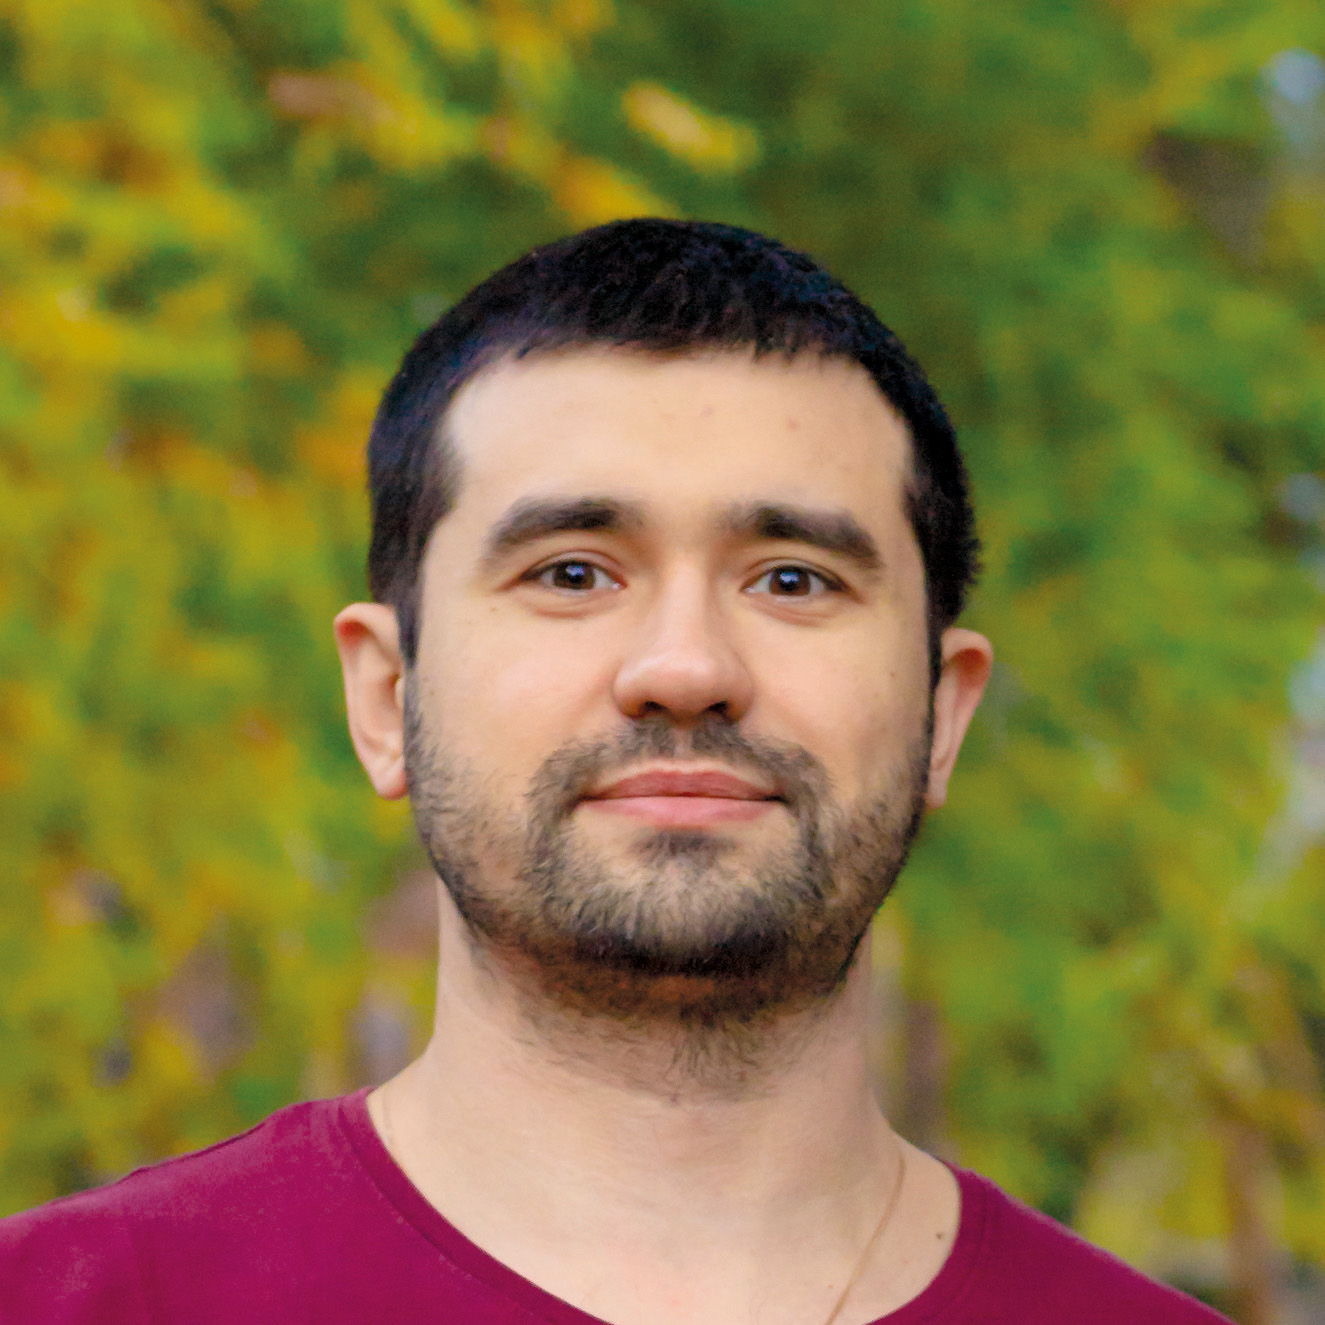
\includegraphics[width=2cm, height=2cm]{media/avatar_rgb.jpg}};
\end{tikzpicture}

\end{minipage}

&
  \vspace{0.25cm}
  {\Large\textbf{Об авторе}}

\end{tabular}

{\small

\noindent
Иван Гришаев~--- увлеченный программист. Последние восемь лет занимается языком
Clojure и редактором Emacs. Работает удаленно в стартапе Audience
Republic. Ведет блог о программировании и удаленной работе \SITELINK.
}

\else

\begin{tabular}{ @{}p{2.5cm} @{}p{5cm} }

\begin{minipage}{2.5cm}
\begin{tikzpicture}
\clip (0,0) circle (1cm) node {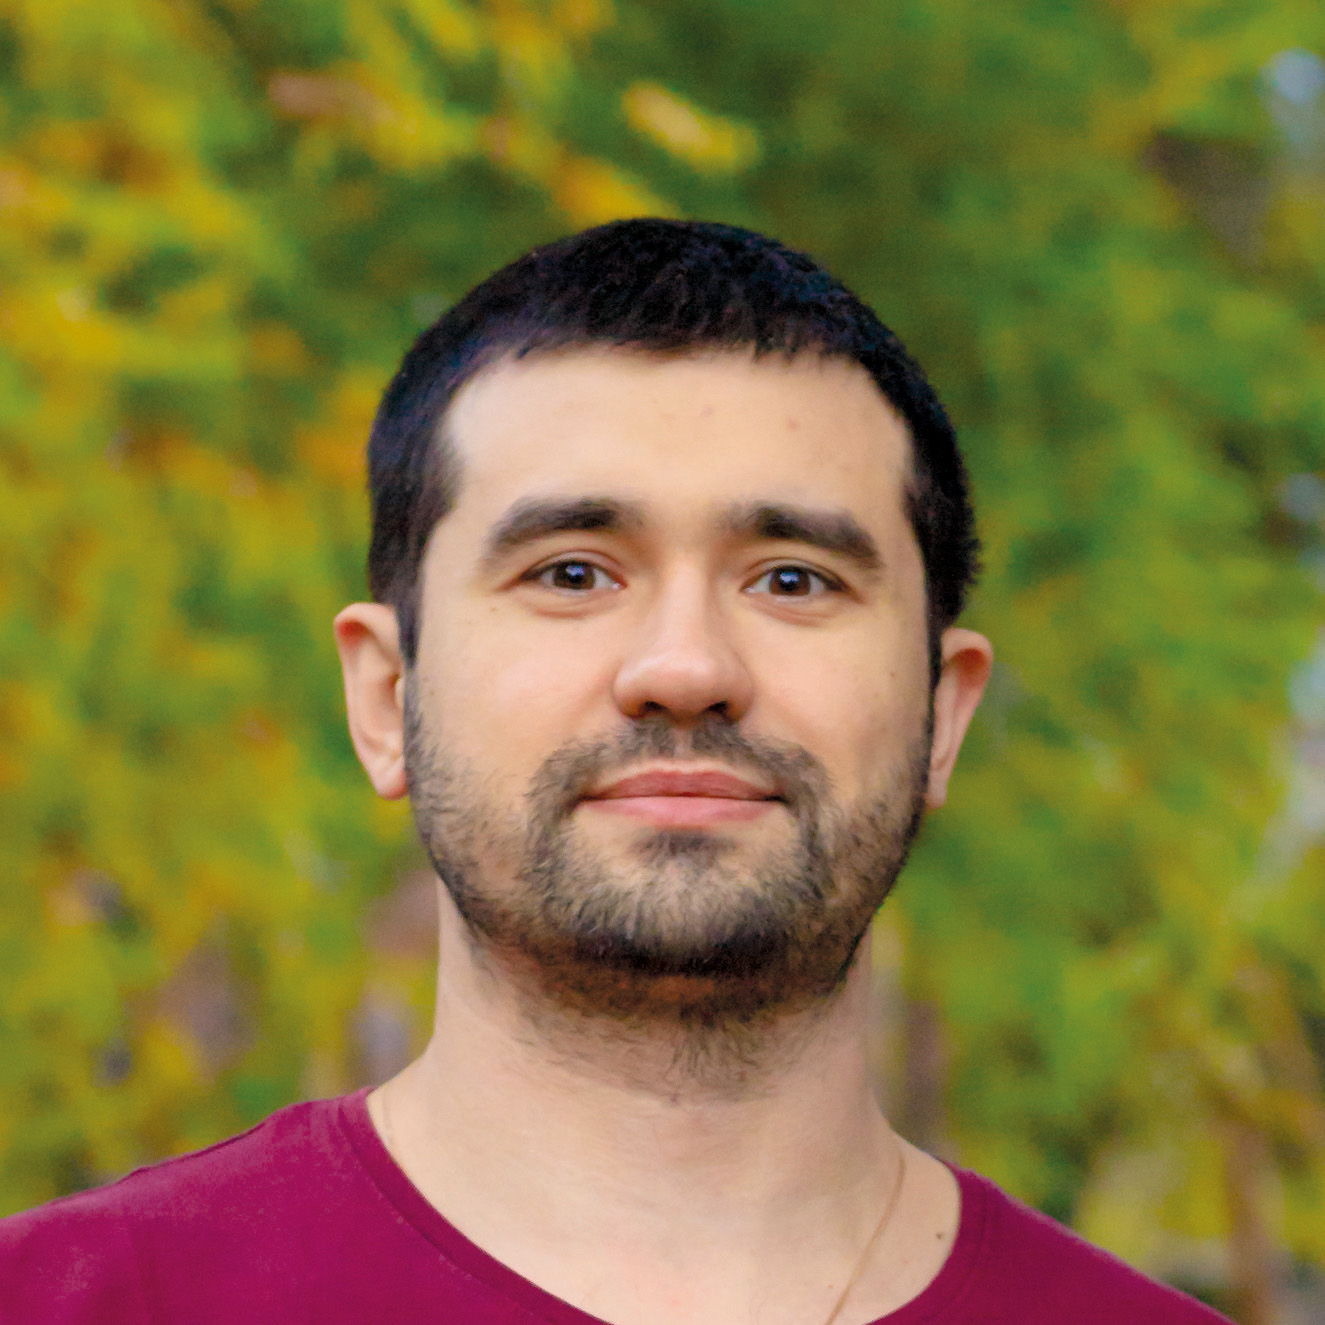
\includegraphics[width=2cm, height=2cm]{media/avatar_rgb.jpg}};
\end{tikzpicture}

\end{minipage}

&

\vspace{-1cm}

\section*{Об авторе}

{\small

Иван Гришаев~--- увлеченный программист. Последние восемь лет занимается языком
Clojure и редактором Emacs. Работает удаленно в стартапе Audience
Republic. Ведет блог о программировании и удаленной работе \SITELINK.

}

\end{tabular}
\fi

\fi

\end{document}
